\documentclass[11pt]{amsart}

\usepackage{amsmath,amssymb}
\usepackage{array,tabularx}
\usepackage{graphicx}
\usepackage[colorlinks=true,linkcolor=blue,citecolor=blue,urlcolor=blue]{hyperref}

\numberwithin{equation}{section}
\setlength{\emergencystretch}{2em}

\newtheorem{theorem}{Theorem}[section]
\newtheorem{proposition}[theorem]{Proposition}
\newtheorem{lemma}[theorem]{Lemma}
\newtheorem{corollary}[theorem]{Corollary}
\theoremstyle{definition}
\newtheorem{definition}[theorem]{Definition}
\theoremstyle{remark}
\newtheorem{remark}[theorem]{Remark}

\newcommand{\R}{\mathbb R}
\newcommand{\T}{\mathbb T}
\newcommand{\J}{\mathbb J}
\newcommand{\cH}{\mathcal H}
\newcommand{\cR}{\mathcal R}
\newcommand{\cU}{\mathcal U}
\newcommand{\cV}{\mathcal V}
\newcommand{\cA}{\mathcal A}
\newcommand{\cE}{\mathcal E}
\newcommand{\cG}{\mathcal G}
\newcommand{\sfC}{\mathsf C}
\newcommand{\Fix}{\operatorname {Fix}}
\newcommand{\dist}{\operatorname {dist}}
\newcommand{\spec}{\operatorname {spec}}
\newcommand{\cut}{\mathrm{cut}}
\newcommand{\alg}{\mathrm{a}}
\newcommand{\pole}{\mathrm{p}}
\newcommand{\out}{\mathrm{out}}
\newcommand{\rbox}{\mathrm{rbox}}
\newcolumntype{Y}{>{\raggedright\arraybackslash}X}

\title[First returns, singular exits, and action finite parts]
{First returns, singular exits, and action finite parts
near a reversible Hamiltonian saddle-focus}
\author{Haibo Lu}
\email{hblu1985@163.com}
\subjclass[2020]{Primary 37J46; Secondary 37B10, 34E15, 37M21}
\keywords{reversible Hamiltonian system, saddle-focus homoclinic orbit,
first-return map, first-exit problem, countable Markov shift,
Hamiltonian action, computer-assisted proof}
\hypersetup{
  pdftitle={First returns, singular exits, and action finite parts near a reversible Hamiltonian saddle-focus},
  pdfauthor={Haibo Lu},
  pdfkeywords={reversible Hamiltonian system, saddle-focus homoclinic orbit, first-return map, first-exit problem, countable Markov shift, Hamiltonian action, computer-assisted proof}
}
\date{}

\begin{document}

\begin{abstract}
We consider a four-dimensional reversible exact Hamiltonian flow whose
saddle-focus germ is real analytic in the state variables and has a
transverse homoclinic orbit.  A fixed local flow tube has two
noncompact forward exits of different types: an algebraic end reached in
infinite physical time and a regular-singular pole reached in finite time.
Assuming a clean limiting first-hit arrangement, normal expansion with
order-three bunching at the algebraic boundary, and a fixed conjugacy class
of indicial operators with simple positive-integer spectrum at the pole, we prove that every orbit
with sufficiently long saddle residence in a fixed compact subcell of the
prescribed source cell belongs to exactly one first-return domain or one
first-exit stratum.  The local exact
symplectic coordinates used in the
proof are constructed from these geometric data and need not exist
globally over the parameter space.

For a compact $C^r$ family $(H_p)_{p\in\mathcal P}$, $0\le r\le2$, the normalized return
maps, flight times, and physical Hamiltonian actions have all mixed
derivatives $D_z^iD_p^j$, $i+j\le2$, $j\le r$, and converge with error
$O((1+n)^3e^{-\kappa n})$ for every
$0<\kappa<\inf_{p\in\mathcal P}2\pi\alpha_p/\beta_p$.  At the algebraic
end, the time and action finite parts are obtained by comparing trajectories
at the same compactifying coordinate.  At the pole, physical flight time
has an ordinary finite limit, while the action finite part is obtained at
fixed remaining physical time by subtracting the Laurent--log terms
determined by the boundary jet.  The two action finite parts are compatible
with exact composition along
concatenated orbit segments and with changes of local coordinates.

The return domains consequently carry a countable Markov coding with
summable-variation roof and action functions, yielding quantitative
period, action, and entropy asymptotics.  Exact calculations and interval
enclosures verify the hypotheses for the normal form associated with a
reversible folded saddle-node of type II.  The conclusion persists in the
relative coefficient topology of the fixed flow tube and end structures
specified in the paper.
\end{abstract}

\maketitle

\section{Introduction}

\subsection{The geometric problem}

A transverse homoclinic orbit to a Hamiltonian saddle-focus creates
return strips with arbitrarily long residence near the equilibrium.  The
recurrent part of this picture is classical.  We study the complementary
first-hit problem in a fixed flow tube: which points return, which points
leave through a prescribed boundary, and what remains of physical time
and Hamiltonian action when a nonreturning orbit reaches a singular end?
The two ends considered here have genuinely different clocks.  An
algebraic end is approached only as physical time tends to infinity,
whereas a regular-singular pole is reached in finite physical time.

Our concrete application is the normal-form system associated with a
reversible folded saddle-node of type II (RFSN-II),
\begin{equation}\label{eq:core-intro}
 U'=P,\qquad P'=-U^2-V,\qquad V'=Q,\qquad Q'=U.
\end{equation}
With $\lambda=P\,dU-Q\,dV$ and $\omega=d\lambda$, it is exact Hamiltonian:
\[
 \iota_X\omega=dH,\qquad
 H=\frac12(Q^2-P^2)-\frac13U^3-UV,
\]
and it is reversed by
$\cR(U,P,V,Q)=(U,-P,V,-Q)$.  The origin is a saddle-focus with eigenvalues
$(\pm1\pm i)/\sqrt2$, and we work on the critical level $H=0$ through the
origin.  Section~\ref{sec:verification} constructs a transverse symmetric
homoclinic orbit and both noncompact forward channels for this system.

An orbit entering a small saddle-focus neighborhood may remain there for
a long time, make an arbitrarily large number of turns, and then reach an
outgoing section.  Some outgoing points traverse the homoclinic tube and
return to the incoming section.  Others reach one of the two noncompact
ends or cross a fixed boundary of the local flow-tube domain.  The question
is whether all sufficiently high-winding initial points can be divided,
without gaps or overlaps, into return domains and first-exit sets, while
retaining estimates uniform both in the winding number and under
perturbation of the Hamiltonian vector field.

We use standard return-map terminology for this geometry.  A \emph{return
strip} is a connected component of the domain of the local first-return
map.  A \emph{first-exit component} is a connected component on which the
first fixed event is arrival at the algebraic end, the pole end, the
stable-manifold cut, or one of the local boundary faces.  Their
disjoint union is the \emph{first-return/first-exit decomposition}.  The
technical sections equip this decomposition with fixed normalized charts,
cross forms, and time/action data; these auxiliary choices are not
additional dynamical objects.
Figure~\ref{fig:return-exit-geometry} summarizes the physical alternatives
and the resulting two-vertex return graph.

\begin{figure}[t]
\centering
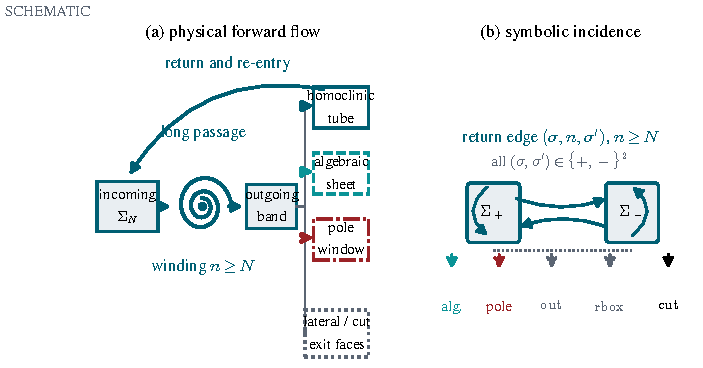
\includegraphics[width=\textwidth]{figures/recurrence_exit_geometry.pdf}
\caption{The fixed local return--exit geometry (schematic, not to scale).
\textup{(a)} A point in the punctured incoming section makes a long
saddle-focus passage.  It either traverses the homoclinic tube and
re-enters the section, or first reaches the codimension-one algebraic
sheet, the open pole window, the stable-manifold cut, or a fixed
lateral face.  Arrows stop at the first fixed event; no subsequent orbit
after a lateral exit is represented.  The algebraic end has infinite
physical flight time, whereas the pole is reached in finite physical
time.  \textup{(b)} Regular returns form a two-vertex countable graph whose
edges are the triples $(\sigma,n,\sigma')$, $n\ge N$, for all four sign pairs.
The first-exit labels are $\mathrm{alg}$ (algebraic end), $\mathrm p$ (pole),
$\mathrm{out}$ (outgoing-box lateral face), $\rbox$ (return-box
lateral face), and $\mathrm{cut}$ (the stable-manifold cut).
In particular, $\mathrm{cut}$ is the zero-action boundary
between the two target-sign return components, not an omitted return edge.
The drawing represents the
fixed flow-tube domain, not a global phase-space partition.}
\label{fig:return-exit-geometry}
\end{figure}

\paragraph{Contributions.}
The main theorem starts from an intrinsic analytic saddle-focus germ, a
transverse physical homoclinic tube, a clean first-hit arrangement, and
geometric compactifications of the two ends.  From these data we construct
local exact symplectic coordinates on a finite cover of parameter space;
no global eigenframe, angle, or winding function is assumed.

The main new conclusion is that the complete collection of labelled
connected strata in the limiting first-hit arrangement persists in every sufficiently
high-winding cell.  On all of these components simultaneously, the return
maps, physical time, and physical action have uniform $C^2$ asymptotics.
The algebraic and pole actions admit finite parts defined by two different
comparison procedures, and both remain compatible with exact composition.
At the pole the finite boundary jet is allowed to vary; a regular-singular
recursion determines the required Laurent--log subtraction.

The return domains also give a countable Markov shift with
summable-variation roof and action functions.  Periodic-orbit asymptotics,
a Lambert-$W$ entropy law, and an $O(L^{-1})$ action-rate estimate follow.
Exact calculations and interval enclosures establish the geometric
hypotheses for the RFSN-II normal form.  The logarithmic saddle-focus
passage, exactness of an individual Poincar\'e branch, and thermodynamic
formalism for a prescribed countable shift are standard ingredients; the
contribution is their uniform compatibility with the exhaustive first-hit
geometry and both singular ends.  The conclusion persists in the relative
coefficient topology of the fixed flow tube and end structures in
Corollary~\ref{cor:core-relative-open-class}.

\subsection{Relation with earlier homoclinic theory}

Transverse Hamiltonian saddle-focus homoclinics already imply finite
horseshoes of arbitrary cardinality \cite{Devaney1976Homoclinic}, and
reversibility yields blue-sky periodic families and multipulse homoclinic
cascades \cite{Devaney1977BlueSky,Harterich1998Cascades}; related
reversible bifocus configurations also support chaotic invariant sets
\cite{BarrientosRaibekasRodrigues2019Chaos}.  The critical
countable admissibility relation and its set-level orbit realization are also
classical \cite{Lerman1991ComplexDynamics,Lerman1997HomoHeteroclinic,
Lerman2000DynamicalPhenomena}.  These results describe recurrent
homoclinic geometry, but they do not give a uniform return/first-exit
decomposition that also resolves the algebraic and pole ends.

The RFSN-II blow-up, its explicit algebraic separatrix, and the associated
canard mechanisms are likewise established \cite{VoDoelmanKaper2025Canards}.
Thus neither the saddle-focus horseshoes nor the RFSN-II ends are new in
isolation.  The point here is to couple them in one local theorem: the
countably many return strips and all complementary first-exit components are
constructed from the vector field, represented in fixed normalized
charts, and controlled together with their flight times and exact actions.
This joint control yields Corollary~\ref{cor:period-action-asymptotics}:
for each fixed cyclic sign pattern it gives the full linear winding term,
an exponentially small remainder, and a limiting closed-orbit action.
Thus, within the prescribed physical flow tube, it refines the qualitative
period-divergence mechanism in the reversible blue-sky setting
\cite{Devaney1977BlueSky} and adds an action asymptotic; it is not a global
classification of blue-sky families.

Bolotin derives a Shilnikov separatrix map for slow--fast Hamiltonian
systems whose frozen dynamics has a transverse saddle-focus homoclinic and
uses it to prescribe the evolution of the slow variables
\cite{Bolotin2025SlowFast}.  Homburg, Lamb, and Turaev obtain positive
topological entropy from strongly transverse symmetric homoclinic tangles
associated with normally hyperbolic families of periodic orbits in smooth
reversible systems \cite{HomburgLambTuraev2025Entropy}.  These results have
natural system-level hypotheses and conclusions extending beyond one
fixed flow tube.  The present theorem is narrower: it resolves every
sufficiently high-winding return and first exit in a prescribed local
domain, and retains the singular time/action data at two different ends.

Countable Markov shifts with summable-variation potentials have an
established thermodynamic theory \cite{Sarig1999Thermodynamic}, while exact
scattering maps for normally hyperbolic invariant manifolds carry
action-based primitives and coboundary laws
\cite{DelshamsDeLaLlaveSeara2008Scattering}.  These are important method
precedents, but both begin after structures that must be constructed here
have already been supplied.  Sarig's theory starts with the countable
alphabet, transition law, and potentials.  Exact scattering maps start
from a normally hyperbolic invariant manifold.  Our task is instead to
construct the shift and its regular potentials from the singular
return/exit geometry, and to prove that both end finite parts are
compatible with the standard exact branch identity.

Rigorous computer-assisted verification of a transverse Hamiltonian
saddle-focus homoclinic in a concrete model was carried out by Kepley and
Mireles James \cite{KepleyMirelesJames2019Chaos}.  Their result illustrates
the distinction maintained here between a general forcing theorem and the
finite validation needed to apply it.  At a different singular scale,
Baldom\'a, Giralt, and Guardia obtain an exponentially small homoclinic
splitting formula by complex matching \cite{BaldomaGiraltGuardia2023L3}.
We do not study separatrix splitting; this comparison emphasizes that the
new quantitative object claimed here is instead the compatibility of the
return/first-exit maps with the two renormalized ends.

\begin{center}
\refstepcounter{table}
\parbox{\textwidth}{\small\textsc{Table \thetable.}
Relation to the closest established frameworks.  The last column states
the additional object constructed here, not a priority claim beyond the
cited scope.\label{tab:literature-comparison}}
\smallskip
\small
\begin{tabularx}{\textwidth}{@{}p{.24\textwidth}YY@{}}
\hline
Framework & Established starting point & Role in the present paper \\
\hline
Saddle-focus homoclinics
& Finite horseshoes and countable set-level symbolic organization near a
homoclinic saddle-focus
& A return family uniform over the Hamiltonian class, together with all first exits
inside one fixed local domain \\
RFSN-II blow-up
& The algebraic separatrix, noncompact scaling, and associated canard
geometry
& Coupling of the algebraic and pole channels to the same return map and
their time/action renormalizations \\
Countable shifts and scattering maps
& Regularity theory for a given countable shift; exact primitives for
scattering maps associated with an NHIM
& Construction of the shift, roof, and exact branch primitives directly
from the return--exit flow geometry \\
\hline
\end{tabularx}
\end{center}

\subsection{Main result and its scope}

The next statement is the geometric form of the main result.  It separates
the dynamical hypotheses from the local coordinates used in the proof.
The precise uniformity, boundary regularity, and parameter dependence are
given in Definition~\ref{def:intrinsic-two-end-data}; the fully normalized
version is Theorems~\ref{thm:main}--\ref{thm:coding-persistence}.

\begin{theorem}[First returns and singular exits]
\label{thm:main-result}
Let $\mathcal P$ be a compact $C^r$ parameter manifold,
$r\in\{0,1,2\}$.  Assume that the family $(H_p)_{p\in\mathcal P}$,
together with its exact primitive, reverser, fixed flow tube, and end data,
satisfies the geometric hypotheses of
Definition~\ref{def:intrinsic-two-end-data}.  In particular, the following
conditions hold uniformly in $p$.
\begin{enumerate}
\renewcommand{\labelenumi}{\textup{(\roman{enumi})}}
\item The critical energy surface contains a real-analytic saddle-focus
with eigenvalues $\pm\alpha_p\pm i\beta_p$, $\alpha_p,\beta_p>0$, and a
transverse homoclinic orbit.
\item A fixed local flow tube has a finite clean first-hit stratification.
Its nonreturn pieces consist of two specified noncompact exits, the
stable-manifold cut, and fixed lateral faces; this list exhausts the
boundary through which a nonreturning orbit can first leave the tube.
\item At the infinite-time algebraic exit, a desingularized flow extends
to a locally maximal normally expanding invariant hypersurface satisfying
the order-three bunching inequalities.  At the finite-time pole, the
desingularized boundary is a regular-singular sink with a fixed indicial
operator whose spectrum is simple and contained in the positive integers.
\end{enumerate}
The same definition fixes the exact primitive and zero energy, the source
cell and its proper angular arc, the algebraic clock and action scalings,
the pole action order, and the regularity of every transition map.  The
saddle and homoclinic coefficients and the algebraic compactification are
$C^k$, $k\ge5$; the event data are $C^3$; the normally expanding
algebraic hypersurface has the mixed-total $C^3$ regularity in
\eqref{eq:intrinsic-algebraic-mixed-regularity}; the saddle germ is
analytic in the state variables; and the pole coefficients have
$C^{m_{\mathrm p}+3}$ regularity.
Fix
\[
 0<\kappa<
 \inf_{p\in\mathcal P}\frac{2\pi\alpha_p}{\beta_p}.
\]
Then a finite cover of $\mathcal P$ carries compatible local exact
symplectic coordinates, and there is a threshold $T_*$ for the time spent
in the saddle block with the following properties.

\begin{enumerate}
\renewcommand{\labelenumi}{\textup{(\alph{enumi})}}
\item After one restriction to a fixed compact source subcell, every point
in that subcell whose saddle residence is at least $T_*$ belongs, without a
gap or overlap, either to a connected
domain of the first-return map or to exactly one first-exit stratum.  In each
local angular coordinate, all sufficiently large winding cells have the
same labelled connected strata and incidence relations as the limiting
first-hit arrangement.

\item On every return component the Poincar\'e map has a uniformly
contracting Shilnikov cross form, and its transverse return coordinate has
scale $\epsilon_n\asymp\exp(-2\pi\alpha_p n/\beta_p)$.  After pullback to
fixed reference cells and application of the respective normalizations,
the cross forms, first-hit maps, flight times, and physical action
integrals have all mixed derivatives $D_z^iD_p^j$, $i+j\le2$, $j\le r$,
and converge with error $O((1+n)^3e^{-\kappa n})$.  The flight time is
normalized by its linear winding term; the two singular ends use the
finite parts in~\textup{(c)}.

\item The algebraic time and action have finite parts when trajectories are
compared at the same compactifying coordinate.  The pole time has an
ordinary finite limit.  Its action has a finite part at fixed remaining
physical time after subtraction of the finite Laurent--log expansion
determined by the boundary jet.  On
every finite Poincar\'e branch
\[
 P_a:\Sigma_a^-\longrightarrow\Sigma_a^+,
 \qquad
 B_a^{\rm phys}(z)=
 \int_0^{\tau_a(z)}\lambda(X)(\Phi^t z)\,dt,
\]
one has
\[
 P_a^*(\lambda|_{\Sigma_a^+})-\lambda|_{\Sigma_a^-}
 =dB_a^{\rm phys}.
\]
These action primitives compose exactly, and both end finite parts obey
the same composition and coordinate-change laws.

\item In every local angular coordinate the return domains give a
two-vertex countable Markov shift with summable-variation roof and action
functions.  On overlaps the first-hit relation, the trapped Poincar\'e
system, closed periods, and closed actions agree.
\end{enumerate}
\end{theorem}

The first-hit arrangement in hypothesis~\textup{(ii)} is an input at the
limiting physical tube.  The persistence theorem proves something
different: every sufficiently high-winding cell has precisely the same
labelled strata and connected components, with no additional component born
under the exponentially small passage perturbation.  Likewise, the
normally expanding hypersurface in~\textup{(iii)} is a standard geometric
hypothesis; the product block, cone, and corridor inequalities used for
the normal-form example are only sufficient criteria for checking it.

\begin{corollary}[The reversible folded saddle-node normal form]
\label{cor:core}
For the Hamiltonian system \eqref{eq:core-intro}, the hypotheses of
Theorem~\ref{thm:main-result} hold on a fixed critical-energy flow tube.
Consequently, for every $\kappa\in(0,2\pi)$ the sufficiently long
saddle-residence region within the fixed compact source subcell has the
exhaustive first-return/first-exit decomposition, the two action finite
parts, exact action composition, and the countable coding described above.
The corresponding roof and action functions satisfy the period,
action-rate, and entropy conclusions of
Corollary~\ref{cor:period-action-asymptotics} and
Theorem~\ref{thm:tail-entropy-action}.

Moreover, the same conclusion holds for the relatively open family in
Corollary~\ref{cor:core-relative-open-class}; that topology fixes the
physical block and tubes, the cooriented event germs, the algebraic
boundary factorizations and invariant faces, the analytic saddle class,
and the pole action order and indicial class.  This is relative openness,
not ambient openness among unrestricted Hamiltonian systems.
The exact and interval arguments establishing the normal-form hypotheses
are given in Section~\ref{sec:verification} and
Appendix~\ref{app:computer-proof}.
\end{corollary}

Theorem~\ref{thm:local-chart-production} constructs the local exact
symplectic coordinates used in the proof.  Theorem~\ref{thm:main} is the
complete weighted and parameter-dependent statement,
Theorem~\ref{thm:time-action} treats the two end finite parts, and
Theorem~\ref{thm:change-of-marking} proves independence of the compatible
local descriptions.  Period, action, and entropy asymptotics are stated
separately because they are consequences rather than hypotheses of the
return--exit theorem.

This is not an additional existence theorem for a horseshoe.  Classical
saddle-focus homoclinic theory provides finite horseshoes, and earlier work
gives a set-level countable admissibility relation, but neither identifies
the complement of the return domains nor controls flight time and
Hamiltonian action at the two noncompact exits considered here.  The
logarithmic local passage and the transverse homoclinic map produce one
return strip for each sufficiently large winding and source--target sign
pair; transverse first-hit hypersurfaces exhaust the complement; and the
algebraic and pole asymptotics give finite $C^2$ time and action limits
after the stated subtractions.  Because the action is integrated along the
physical orbit, its branch primitives compose exactly, and the same return
domains give the countable Markov coding and summable-variation roof and
action functions.  The conclusion is local to the prescribed physical
flow tube and its long-passage collar.  The coordinate estimates exclude
local windings $n_i<N_i$ and retain the fixed pole indicial conjugacy class.

The upper rate
$\inf_{p\in\mathcal P}\frac{2\pi\alpha_p}{\beta_p}$ is geometric.  In a local
marking, a branch of
winding $n$ spends time
\[
 T_n\sim\frac{2\pi}{\beta_{\mathbf X}}n
\]
near the saddle-focus, so its transverse scale is
\[
 e^{-\alpha_{\mathbf X}T_n}
 \sim\exp\left(-\frac{2\pi\alpha_{\mathbf X}}
                    {\beta_{\mathbf X}}n\right).
\]
Fixing
$\kappa<\inf_{p\in\mathcal P}\frac{2\pi\alpha_p}{\beta_p}$ leaves the uniform strict rate
gap needed for two-jet estimates on the finite parameter cover.  For the
normal-form system \eqref{eq:core-intro}, $\alpha_0=\beta_0$, and the
upper exponent is $2\pi$.  We do not claim uniform constants as
$\kappa\uparrow
 \inf_{p\in\mathcal P}\frac{2\pi\alpha_p}{\beta_p}$.

The result is local to the fixed flow tube and its long-passage region: a
lateral exit makes no assertion about the subsequent orbit, and low
windings are excluded.  The local angular cuts and winding labels need not
globalize, and a one-sided symbolic word determines a stable plaque rather
than a single point.  Section~\ref{sec:scope} records the remaining scope
limits in one place.

\subsection{Proof strategy}

The proof separates local coordinate construction, the saddle-focus
passage, the finite first-hit geometry, and the two end compactifications.

\paragraph{Local coordinates and long passages.}
Local spectral trivializations, equivariant exact Darboux coordinates, and
the reversible analytic normal form produce transverse sections with exact
action-angle coordinates and a flight-time function.  Event-free orbit
slides connect them to the physical faces.  In these coordinates the long
saddle passage is a mixed boundary-value problem: stable data are imposed
at the incoming end and unstable data at the outgoing end.  Volterra
estimates give the orbit and its mixed two-jets.  Comparing its action with
the two limiting half-orbit integrals leaves an exponentially small
interaction term.

\paragraph{Matching and the complete first-hit partition.}
The logarithmic phase of the local passage and the finite homoclinic map
give a matching equation.  The implicit-function theorem produces the
high-winding return strips and their contracting Shilnikov cross forms on
the scale $\exp(-2\pi\alpha n/\beta)$.  Local implicit graphs alone do not
give exhaustiveness.  That step uses whole-cell $C^2$ convergence and a
controlled isotopy of the clean, neat first-hit stratifications to obtain a
bijection of connected strata; strict first-hit margins preserve event
order.  Hence no additional high-winding component is hidden between the
constructed return and exit sets.

\paragraph{Finite parts, exact composition, and coordinate changes.}
At the algebraic end, an escaping orbit and a fixed reference orbit are
compared at the same compactifying coordinate.  At the pole, physical
remaining time is the asymptotic variable and a regular-singular recursion
determines the Laurent--log subtraction.  The remaining time and action
terms have uniform mixed $C^2$ limits.  Because action is always the
physical integral $\int\lambda(X)\,dt$, it composes exactly before the
limit.  Changes of section or primitive add endpoint coboundaries; changes
of angular cut give bounded winding recodings.  A finite common refinement
therefore identifies the physical first-hit relation, trapped system,
closed periods, and closed actions on chart overlaps.

\paragraph{Coding and the normal-form application.}
The cross-form equations define a contraction on sequence space and hence
a countable Markov coding; exponential dependence on the first differing
symbol gives summable variations.  The entropy and action-rate estimates
are consequences of this coding.  Exact calculations and interval
enclosures establish the geometric hypotheses for
\eqref{eq:core-intro}; their strict margins yield the relative-open family
of Corollary~\ref{cor:core-relative-open-class}.  The selected reversible
branch and its restricted-Hamiltonian critical points are a separate
consequence, not an input to the return--exit theorem.

Sections~2--3 formulate the geometric hypotheses, construct the local
coordinates, and state the quantitative results.  Sections~4--7 prove the
passage, first-hit, finite-part, and coding statements; Section~8 treats the
normal-form application.  Appendix~\ref{app:algebraic-interval-criterion}
gives the computable interval-block test for the algebraic hypersurface;
weighted function spaces, validation records, uniform end limits, and the
optional Jost calculation occupy the remaining appendices.

\paragraph{Dependency map.}
Table~\ref{tab:proof-dependency} separates the logical input/output layers
of the main theorem from the optional modules.  Its short package codes are
expanded immediately below; Appendix~\ref{app:computer-proof} gives the
exact certificate paths and quantitative margins.

\begin{center}
\refstepcounter{table}
\parbox{\textwidth}{\small\textsc{Table \thetable.}
Hypotheses, theorem outputs, and computational dependencies.  The optional
rows are not in the logical dependency chain of
Theorem~\ref{thm:main-result} or Corollary~\ref{cor:core}.
\label{tab:proof-dependency}}
\smallskip
\small
\begin{tabularx}{\textwidth}{@{}
  >{\raggedright\arraybackslash}p{.23\textwidth}
  Y
  >{\raggedright\arraybackslash}p{.27\textwidth}@{}}
\hline
Input layer & Mathematical output & RFSN-II validated evidence
(supplementing exact identities; rows may overlap) \\
\hline
Analytic saddle and transverse homoclinic, \textup{(I1)}--\textup{(I2)}
& Parameter-local exact symplectic charts, the long saddle passage, and
the matching graph
& M3 \\
Clean event geometry, \textup{(I3)}
& Persistence of the prescribed limiting census, with no new component,
on every sufficiently long-residence cell
& Jointly M1--M4 \\
Algebraic compactification, \textup{(I4)}
& Local graph representation and persistence of the supplied normally
expanding hypersurface; algebraic time/action finite parts
& M1, M2 \\
Regular-singular pole, \textup{(I5)}
& Pole entry, finite remaining time, and the intrinsic Laurent--log action
finite part
& M4 \\
The preceding four rows
& Theorem~\ref{thm:main-result}, its exact cocycle, coding, and
Corollary~\ref{cor:core}
& M1--M4, plus the provenance audit during replay \\
Optional general selected-branch theorem
& Corollary~\ref{cor:source-fold-persistence} and its analytic proof
& No certificate dependency \\
Optional normal-form selected branch
& Proposition~\ref{prop:exact-source-outer-fold},
Corollary~\ref{cor:core-selected-branch}, and
Appendix~\ref{app:jost-source-arm}
& S1--S5; none is a main-theorem dependency \\
Optional restricted matching genericity
& Section~\ref{sec:matching-genericity}
& Analytic perturbation argument; no certificate dependency \\
\hline
\end{tabularx}
\end{center}

\begingroup\small
\noindent
M1: \path{future-target-fold};
M2: \path{origin-algebraic-heteroclinic};
M3: \path{universal-core-symmetric-homoclinic};
M4: \path{origin-unstable-pole-entry}.
The codes S1--S5 denote, in the order printed in
Appendix~\ref{app:computer-proof}, the five additional claim-bearing
packages for the optional normal-form selected branch.  The complete
\texttt{all} replay also runs two ancillary packages and the
\path{toolchain-metadata-audit} node; these do not supply hypotheses of the
main theorem.
\endgroup

Figure~\ref{fig:proof-dependency} summarizes this route and separates the
analytic construction from the normal-form verification.
\begin{figure}[tbp]
\centering
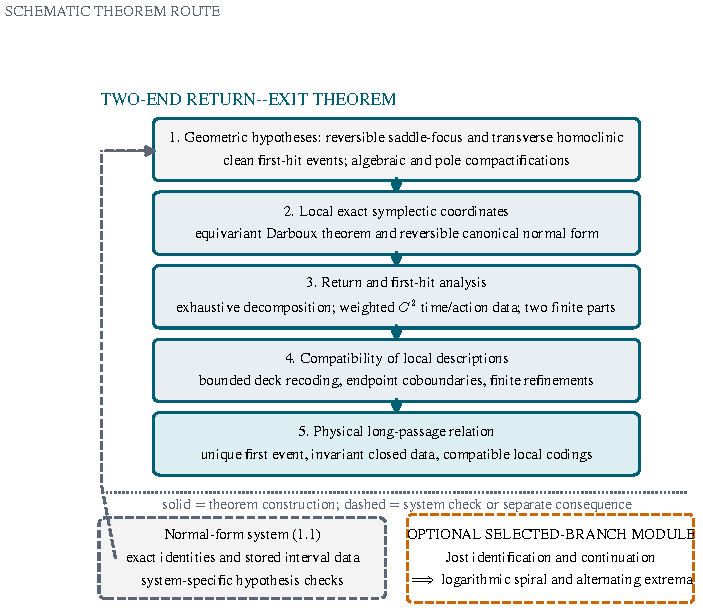
\includegraphics[width=\textwidth]{figures/proof_dependency.pdf}
\caption{Route through the theorem.  Intrinsic physical data produce a
finite parameter-local family of reversible exact symplectic coordinates.  The
local analytic construction gives the return/first-exit, time, action, and
end data; compatible coordinate changes identify these descriptions as one
physical long-passage relation.  Neither end is derived from the
saddle-focus germ, and no global winding label is asserted.  The dashed
arrow records exact and interval verification of the intrinsic hypotheses
for \eqref{eq:core-intro}.  The selected reversible branch is an optional
consequence using the Jost identification and finite continuation.  The
diagram is schematic and is not an exhaustive dependency graph.}
\label{fig:proof-dependency}
\end{figure}

\section{Geometric hypotheses and local exact symplectic coordinates}

\subsection{Geometric data}

The return--exit theorem is proved in coordinates, but its geometric input
need not include those coordinates.  We therefore distinguish a physical
configuration from a \emph{marked representation} of that configuration.
The definition below deliberately retains the two compactified ends and the
event hypersurfaces as geometric hypotheses: they are not consequences of a
saddle-focus homoclinic orbit.

\begin{definition}[Intrinsic two-ended Hamiltonian configuration]
\label{def:intrinsic-two-end-data}
Let $\mathcal P$ be a compact $C^r$ parameter manifold,
$r\in\{0,1,2\}$.  An intrinsic two-ended configuration over $\mathcal P$
consists of a fixed exact symplectic four-manifold $(M,d\lambda)$ with an
anti-symplectic involution $\mathcal R$ and a chosen physical primitive
satisfying
\[
 \mathcal R^*\lambda=-\lambda,
\]
an integer $m_{\mathrm p}\ge2$, a conjugacy class of real
$3\times3$ matrices whose spectrum is simple and contained in the positive
integers
\begin{equation}\label{eq:intrinsic-pole-spectrum}
 \Lambda_{\mathrm p}=\{\lambda_1<\lambda_2<\lambda_3\}
 \subset\mathbb N,
\end{equation}
and a $C^r$ family of
$\mathcal R$-invariant Hamiltonians $H_p$, $p\in\mathcal P$, with the
following data and hypotheses.
All compactifications, bundles, submanifolds, boundary defining functions,
fields, bundle atlases, splittings, metrics, and first-hit maps listed below
form parameter-locally trivial $C^r$ families in the displayed $C^3$,
$C^k$, or $C^{m_{\mathrm p}+3}$ state norms, except for the normally expanding
hypersurface in \textup{(I4)}.  Parameter-locally write that hypersurface
as a normal section $\Gamma_p$ over a fixed domain; its required regularity
is the mixed-total scale
\begin{equation}\label{eq:intrinsic-algebraic-mixed-regularity}
 \sup_{\substack{i+j\le3\\j\le r}}
 \|D_z^iD_p^j\Gamma_p\|<\infty.
\end{equation}
All strict inequalities and
compactness statements are uniform over $p\in\mathcal P$.
\begin{enumerate}
\renewcommand{\labelenumi}{\textup{(I\arabic{enumi})}}
\item \emph{Analytic saddle-focus and physical saddle block.}
There is a $C^r$ family $O_p\in\Fix\mathcal R$ of critical points on
$H_p^{-1}(0)$ such that
\[
 \spec DX_{H_p}(O_p)=\{\pm\alpha_p\pm i\beta_p\},
 \qquad
 \inf_{p\in\mathcal P}\min\{\alpha_p,\beta_p\}>0.
\]
The saddle neighborhoods carry parameter-locally trivial real-analytic
structures in which $d\lambda$, a local representative of $\lambda$, and
$\mathcal R$ are real analytic.  The germs of $H_p$ at $O_p$ are real
analytic in the state variables on parameter-locally uniform complex
neighborhoods and, together with these analytic symplectic and reversible
data, depend $C^r$ on $p$ in the corresponding analytic norms.  A fixed physical saddle block
$\mathcal B_{\mathrm{sf},p}$ is supplied with transverse incoming and
outgoing faces $S^s_p,S^u_p$.  The first-hit time across this block is
denoted by $\mathcal T_{\mathrm{sf},p}$; the faces and the block vary
$C^r$ with $p$.  Its punctured long-passage collar contains no event face,
so auxiliary transverse sections inside the block may be joined to the
physical faces by event-free orbit slides with uniformly bounded times and
mixed derivatives through order three.

\item \emph{Transverse homoclinic tube.}
There is a $C^r$ family of selected homoclinic orbits $\gamma_p$ and a
compact $C^k$, $k\ge5$, family of flow tubes containing a fundamental
segment of each $\gamma_p$; $H_p$ and $X_{H_p}$ are $C^k$ in the state
variables on these tubes and $C^r$ in $p$ in the corresponding norms.
Along that segment,
\begin{equation}\label{eq:intrinsic-homoclinic-transversality}
 T_zW^s(O_p)+T_zW^u(O_p)=T_zH_p^{-1}(0).
\end{equation}
The finite homoclinic flight from $S^u_p$ to $S^s_p$ has a uniform
first-hit margin.

\item \emph{Physical event arrangement.}
The incoming face carries a compact physical source cell whose boundary is
transverse to the phase-circle fibers of the oriented blow-up and contains
the homoclinic and the two designated end-anchor projections in its
interior.  The cell is local in the phase direction: on the oriented
blow-up, the union of its two signed limiting residual-phase traces and the
designated anchor traces is contained, parameter-locally, in an open arc
bundle whose complementary arc has positive uniform length.  This
proper-arc condition is unchanged by a degree-one reparametrization of the
phase-circle fibers.  The theorem concerns this one local source cell; a
larger phase cover is not asserted.
The compact return--exit tube carries a finite $C^3$ family of cooriented
event hypersurface germs.  Together with the return aperture, these event
faces exhaust the relevant outgoing boundary of the fixed tube: an orbit
that leaves before returning has a prescribed first hit.  The connected
pure-dimensional strata on the outgoing band and, inside the homoclinic
aperture, the strata obtained after pulling back the return-band
arrangement form a finite exhaustive list.  Each relative interior is
assigned exactly one outcome: genuine return, pole or algebraic exit,
outgoing- or return-box lateral exit, or the stable-manifold cut.  There is
no residual component, and a fixed priority assigns an outcome on common
faces and corners without merging dimensions.  On the oriented real
blow-up of the stable and unstable axes, their limiting pullbacks and the homoclinic aperture form a
finite clean stratification, neat at the boundary faces.  Assigned first
hits are transverse, and the inactive-face and strict event-order
inequalities have positive uniform margins.  The limiting algebraic and
pole strata each contain a specified interior point with positive boundary,
inactive-face, and event-order margins.  Cleanliness here is independent of
a local eigenframe: two such frames act on the boundary circle bundle by a
degree-one diffeomorphism.

\item \emph{Algebraic compactification.}
The algebraic channel has a $C^k$ manifold-with-boundary compactification
$\overline M_{\mathrm a,p}$,
a boundary defining function $e$, and a desingularized field
$Y_{\mathrm a,p}$ satisfying
\begin{equation}\label{eq:intrinsic-algebraic-data}
 \frac{dt}{ds}=e^{1/2}\widehat\chi_{\mathrm a,p},\qquad
 Y_{\mathrm a,p}e=e^2v_{e,p},\qquad v_{e,p}<0,
\end{equation}
with uniform bounds, while $E=2H_p$ and
$e^3\lambda(X_{H_p})$ extend with the stated $C^k$ regularity.  The
extension of $E$ is a submersion defining the boundary energy face.
Inside the boundary energy face there is a cooriented invariant flag with
one-dimensional normal quotient whose desingularized linear rate is
uniformly negative.  Equivalently, a local defining function $b$ for that
flag satisfies, by Hadamard's lemma,
\[
 Y_{\mathrm a,p}b=e f_{e,p}+E f_{E,p}+b v_{b,p},
 \qquad v_{b,p}<0,
\]
on a sufficiently small collar.
Along the common flag, $(de,dE,db)$ is a clean defining system: its
conormals are linearly independent with a positive uniform least singular
value.  On a fixed collar this system extends as a rank-three submersion.
There is a compact $C^3$ locally invariant hypersurface with boundary
$\mathcal W^{\rm tail}_{\mathrm a,p}$ in this collar.  It is locally
maximal on a compact relative isolating neighborhood: the points whose
positive semiorbits remain in that neighborhood are precisely
$\mathcal W^{\rm tail}_{\mathrm a,p}$.  The restriction of $(e,E,b)$ to
this hypersurface is a $C^3$ diffeomorphism onto a compact base domain
$B_p$ with corners whose interior contains $(e_*,0,0)$ for a fixed
$e_*>0$.  Every tangential boundary face is strictly inward or
structurally invariant.  For some $\delta_{\mathrm a}>0$, let
 $\Phi_p^s$ denote the flow of $Y_{\mathrm a,p}$ and set
\begin{align*}
 A^{\delta}_{p,z}
 &=D\Phi_p^{\delta_{\mathrm a}}|_{T_z\mathcal W^{\rm tail}_{\mathrm a,p}},\\
 N^{\delta}_{p,z}
 &:T_z\overline M_{\mathrm a,p}/T_z\mathcal W^{\rm tail}_{\mathrm a,p}
   \longrightarrow
   T_{\Phi_p^{\delta_{\mathrm a}}z}\overline M_{\mathrm a,p}/
   T_{\Phi_p^{\delta_{\mathrm a}}z}\mathcal W^{\rm tail}_{\mathrm a,p}.
\end{align*}
With continuous adapted metrics, this hypersurface is normally expanding
in forward desingularized time and is order-three bunched:
\begin{equation}\label{eq:intrinsic-algebraic-normal-bunching}
 \vartheta_{\mathrm a,j}:=
 \sup_{p,z\in\mathcal W^{\rm tail}_{\mathrm a,p}}
 \bigl\|(N^\delta_{p,z})^{-1}\bigr\|
 \bigl\|A^\delta_{p,z}\bigr\|^j<1,
 \qquad j=0,1,2,3.
\end{equation}
Here $j=0$ is normal expansion and $j=1,2,3$ are the standard bunching
conditions for persistence with three derivatives.

The interval-block hypotheses in
Theorem~\ref{thm:algebraic-corridor-graph} give a computable sufficient
criterion for the existence, local maximality, and bunching of this
hypersurface.  The product trivialization and its cone estimates are not
part of the intrinsic hypothesis.
A physical cut $e=e_*$ in the interior of the collar and a finite
first-hit/saturation map from a fixed open neighborhood of the whole
compact cut slice to the algebraic event face are part of the data, with
compact closure and uniform first-hit and coorientation margins.  Its
domain contains a fixed neighborhood of
$\mathcal W^{\rm tail}_{\mathrm a,p}\cap\{e=e_*\}$.

\item \emph{Pole compactification.}
The pole channel has a $C^{m_{\mathrm p}+3}$
manifold-with-boundary compactification with
boundary defining function $\rho$.  The desingularized physical field
$\rho X_{H_p}$ extends to a hyperbolic boundary sink $q_{\infty,p}$, and
\[
 d\rho(\rho X_{H_p})=\rho a_p,\qquad a_p(q_{\infty,p})<0.
\]
On the intrinsic tangential quotient at the sink, the regular-singular
endomorphism
\begin{equation}\label{eq:intrinsic-pole-indicial-map}
\mathcal I_p=a_p(q_{\infty,p})^{-1}
 D(\rho X_{H_p}|_{\partial})_{q_{\infty,p}}
\end{equation}
has the fixed conjugacy class specified above, with spectrum
$\Lambda_{\mathrm p}$ in \eqref{eq:intrinsic-pole-spectrum}.
The coefficient $\rho^{m_{\mathrm p}}\lambda(X_{H_p})$ extends in
$C^{m_{\mathrm p}+3}$, and the pole
entrance has compact image in the basin of the sink with uniform entry,
radial, and spectral-gap margins.
\end{enumerate}
All objects above are physical submanifolds, compactifications, invariant
hypersurfaces, or finite-time tangent-cocycle inequalities.  The
definition contains no eigenframe, angle lift, sign or winding label,
matching graph, return strip, or renormalized end potential.  In a
concrete application the future-staying hypersurface may instead be
constructed from the interval-block criterion in
Appendix~\ref{app:algebraic-interval-criterion}.
\end{definition}

For later comparison, in a fixed product bundle chart with product
connection,
$DY=\left(\begin{smallmatrix}C&B\\D&a\end{smallmatrix}\right)$ and
$P=\operatorname{graph}S$, $\|S\|\le\alpha$.  If
$\mu_2(C)\le c$ and $\|B\|\le b$ in the adapted metrics, then
\begin{align}
 L(P)&=C+BS,& n(P)&=a-SB,
 \label{eq:intrinsic-to-block-rates}\\
 n(P)-j\mu(L(P))&\ge a-jc-(j+1)b\alpha .&&\notag
\end{align}
If the right-hand side is bounded below by $\gamma_j>0$ along every
$\delta_{\mathrm g}$-admissible evolving plane, integration gives
$\vartheta_{\mathrm g,j}\le e^{-\gamma_j\delta_{\mathrm g}}$.
Thus the block inequalities used in the RFSN-II verification are a
computable chartwise sufficient criterion for
\eqref{eq:alg-intrinsic-rate-gaps}; they are not part of the intrinsic
definition.

\subsection{Exact reversible fields and local coordinate descriptions}

Let $(M,\lambda)$ be an exact symplectic four-manifold,
$\omega=d\lambda$, and let $\cR$ be an anti-symplectic involution.  We use
the convention
\begin{equation}\label{eq:exact-reversible}
 \iota_X\omega=dH,\qquad H\circ\cR=H,\qquad
 \cR^*\lambda=-\lambda,\qquad \cR_*X=-X.
\end{equation}
A \emph{marked Hamiltonian presentation} is the datum
\begin{equation}\label{eq:marked-germ}
 \mathbf X=(X,H,\lambda,\cR;
       \Xi_{\mathrm{sf}},\Xi_{\mathrm{fin}},
       \Xi_{\mathrm a},\Xi_{\mathrm p}),
\end{equation}
with fixed chart domains and fixed transition maps on their overlaps.  The
equilibrium is marked by $O=0$ and $H(O)=0$.

In the saddle-focus chart the field has reversible cross form
\begin{equation}\label{eq:sf-cross-form}
 \dot\xi=A_{\mathbf X}\xi+F_{\mathbf X}(\xi,\eta),
 \qquad
 \dot\eta=-A_{\mathbf X}\eta+G_{\mathbf X}(\xi,\eta),
 \qquad
 A_{\mathbf X}=\alpha_{\mathbf X}I+
                  \beta_{\mathbf X}\J,
\end{equation}
where $\alpha_{\mathbf X},\beta_{\mathbf X}>0$, $\J$ is the standard
complex structure on $\R^2$, the reverser exchanges $\xi$ and $\eta$, and
\begin{equation}\label{eq:axis-vanishing}
 F(\xi,0)=F(0,\eta)=G(\xi,0)=G(0,\eta)=0.
\end{equation}
The four vanishing relations are recorded by Hadamard coefficients in the
two variables.  The compact chart contains a fixed finite union
$K_{\mathrm{fin}}$ of flow-tube boxes: the primary homoclinic tube, the
finite part of the algebraic connection, the pole-entry tube, and the
outgoing, return, and boundary collars used below.

The saddle-focus marking contains one further, genuinely Hamiltonian piece
of data.  On fixed exact-symplectic incoming and outgoing section charts,
and on each component $\sigma\nu>0$ of the critical energy, the exact local
passage is required to be
\begin{equation}\label{eq:marked-moser-passage}
 \mathcal L_{\mathbf X,\sigma}(\phi,\nu)
   =\bigl(\phi+\Delta_{\mathbf X,\sigma}(\nu),\nu\bigr),
 \qquad
 \Delta_{\mathbf X,\sigma}(\nu)
   =\frac{\beta_{\mathbf X}}{\alpha_{\mathbf X}}\log|\nu|
      +b_{\mathbf X,\sigma}+\rho_{\mathbf X,\sigma}(\nu).
\end{equation}
Thus equality of the two action coordinates is exact, not an asymptotic
claim.  With $D_{\log\nu}:=\nu\partial_\nu$, the marked remainder obeys
\begin{equation}\label{eq:marked-moser-remainder}
 \max_{0\le j\le k-2}\sup_{0<|\nu|\le\nu_*}
 \frac{|D_{\log\nu}^j\rho_{\mathbf X,\sigma}(\nu)|}
 {|\nu|(1+|\log|\nu||)}<\infty.
\end{equation}
The same actual local passage, in the same section charts, carries the
physical flight-time law
\begin{equation}\label{eq:marked-flight-time}
 T_{\mathbf X,\sigma}(\nu)
 =-\frac1{\alpha_{\mathbf X}}\log|\nu|
    +t_{\mathbf X,\sigma}+\tau_{\mathbf X,\sigma}(\nu),
 \qquad
 c_{\mathbf X,\sigma}:=e^{\alpha_{\mathbf X}t_{\mathbf X,\sigma}}
 \ge c_*>0,
\end{equation}
where
\begin{equation}\label{eq:marked-time-remainder}
 \max_{0\le j\le k-2}\sup_{0<|\nu|\le\nu_*}
 \frac{|D_{\log\nu}^j\tau_{\mathbf X,\sigma}(\nu)|}
 {|\nu|(1+|\log|\nu||)}<\infty.
\end{equation}
Thus $c_{\mathbf X,\sigma}$ is derived from the exact local flight time,
not an independently chosen coefficient.  The map
\eqref{eq:marked-moser-passage} and the clock
\eqref{eq:marked-flight-time} are two components of the same marked local
flow.  They are local section data; no return orbit is used to define them.

At the algebraic end use coordinates
$z_{\mathrm a}=(e,E,b,\zeta)$, where $E=2H$.  The physical field is still
denoted by $X$, but the regular compactified field is the desingularization
\[
 Y_{\mathrm a}=\chi_{\mathrm a}X,
 \qquad \frac{dt}{ds}=\chi_{\mathrm a}
 =e^{1/2}\widehat\chi_{\mathrm a},
 \qquad 0<\chi_*\le\widehat\chi_{\mathrm a}\le\chi^*.
\]
Thus $E_s=0$, and a dot in the algebraic chart denotes differentiation
with respect to $s$.  The regular compactified physical action coefficient
is
\begin{equation}\label{eq:alg-density}
 a_{\mathrm a}^{\mathrm c}=e^3\lambda(X).
\end{equation}
The raw coefficient conditions are
\begin{equation}\label{eq:alg-factorization}
 Y_{\mathrm a}^e=e^2v_e,\qquad v_e\le-a_*<0,
 \qquad
 Y_{\mathrm a}^b=e f_e+E f_E+bv_b,
 \qquad v_b\le-\lambda_*<0.
\end{equation}
Fix a compact rectangular base corridor $B_\Gamma$ in the
$x=(e,E,b)$ coordinates and a number $\zeta_\Gamma>0$ such that
\begin{equation}\label{eq:alg-corridor}
 Q_\Gamma=B_\Gamma\times[-\zeta_\Gamma,\zeta_\Gamma]
\end{equation}
has a fixed collar in the algebraic chart.  Write the compactified field
and its derivative in base--normal blocks as
\begin{equation}\label{eq:alg-block-field}
 Y_{\mathrm a,\mathbf X}(x,\zeta)
   =(F_{\mathbf X}(x,\zeta),G_{\mathbf X}(x,\zeta)),
 \qquad
 DY_{\mathrm a,\mathbf X}
 =\begin{pmatrix}C_{\mathbf X}&B_{\mathbf X}\\
                  D_{\mathbf X}&a_{\mathbf X}\end{pmatrix}.
\end{equation}
Here $C_{\mathbf X}$ is a $3\times3$ matrix,
$B_{\mathbf X}$ is a column, $D_{\mathbf X}$ is a row, and
$a_{\mathbf X}=\partial_\zeta G_{\mathbf X}$.  We use the Euclidean
logarithmic norm
\begin{equation}\label{eq:alg-logarithmic-norm}
 \mu_2(C)=\lambda_{\max}\!\left(\frac{C+C^{\mathsf T}}2\right).
\end{equation}
The face, cone, and finite-order rate conditions imposed on these raw
coefficients are stated in
Theorem~\ref{thm:algebraic-corridor-graph}; they are only a sufficient
test for \textup{(H3)}.  In particular, $f_e$ may
be nonzero: no complete reference curve is fixed in the definition of the
class.

At the pole put
\begin{equation}\label{eq:pole-coordinates}
 \rho=x^{-1/2},\qquad A=\rho^3y,\qquad
 B=\rho q,\qquad C=\rho^4w,
 \qquad \frac{d\tau}{dt}=\rho^{-1}.
\end{equation}
For the core, the compactified field is
\begin{equation}\label{eq:pole-field}
 \dot\rho=-\tfrac12A\rho,\qquad
 \dot A=1-\tfrac32A^2-C,\qquad
 \dot B=1-\tfrac12AB,\qquad
 \dot C=-2AC+\rho^4B,
\end{equation}
and has the hyperbolic sink
\begin{equation}\label{eq:pole-sink}
 p_\infty=(0,\sqrt{2/3},\sqrt6,0).
\end{equation}
For a fixed marked coefficient class, choose an integer
$m_{\mathrm p}\ge2$ and a real matrix $\mathcal I$ with simple positive
integral spectrum $\Lambda_{\mathrm p}$ as in
\eqref{eq:intrinsic-pole-spectrum}, and set
\begin{equation}\label{eq:general-compactified-action-order}
 a_{\mathrm p}^{\mathrm c}=\rho^{m_{\mathrm p}}\lambda(X).
\end{equation}
For the normal-form system, $m_{\mathrm p}=6$.  For a general
presentation, use a marked $C^{m_{\mathrm p}+3}$ boundary
chart centered at its pole equilibrium and write
\begin{equation}\label{eq:general-pole-field}
 X_{\mathrm p}
 =\rho a(\rho,u)\partial_\rho+b(\rho,u)\cdot\partial_u,
 \qquad u\in\R^3,\qquad b(0,0)=0.
\end{equation}
The radial coefficient satisfies $a(0,0)<0$.  After a marked linear change
in $u$, the principal regular-singular operator is required to be
\begin{equation}\label{eq:pole-indicial-matrix}
 \mathcal I_X:=a(0,0)^{-1}D_ub(0,0)=\mathcal I,
 \qquad
 \spec\mathcal I=\Lambda_{\mathrm p}\subset\mathbb N,
 \quad \Lambda_{\mathrm p}\ \hbox{simple}.
\end{equation}
For the normal-form system these fixed data are
\begin{equation}\label{eq:core-pole-indicial-matrix}
 m_{\mathrm p}=6,\qquad
 \mathcal I=
 \begin{pmatrix}
  6&0&\sqrt6\\
  3&1&0\\
  0&0&4
 \end{pmatrix},
 \qquad \spec\mathcal I=\{1,4,6\}.
\end{equation}
For the core, take
$u=(A-\sqrt{2/3},B-\sqrt6,C)$ in \eqref{eq:pole-field}; direct
linearization gives \eqref{eq:core-pole-indicial-matrix}.  Fix a relatively
compact neighborhood $U_{\mathrm p}\subset\R^3$ of $u=0$.  For a scalar
or vector coefficient $R$ in this chart, put
\begin{equation}\label{eq:pole-norm}
 \|R\|_{m_{\mathrm p}+3;\mathrm p}
 =\max_{j+|\gamma|\le m_{\mathrm p}+3}
   \sup_{(\rho,u)\in[0,\rho_*]\times U_{\mathrm p}}
   |\partial_\rho^j\partial_u^\gamma R|.
\end{equation}
Only $m_{\mathrm p}$, the radial scaling, and the indicial operator are
fixed.  The
nonlinear boundary coefficients, every positive normal jet of the field,
and the complete boundary jet of $a_{\mathrm p}^{\mathrm c}$ are allowed
to vary.

The positive-integer-spectrum assumption selects a standard resonance class
for which the singular density has an ordinary finite Laurent--log
expansion.  The arguments below apply to every fixed
$(m_{\mathrm p},\mathcal I)$ in this class; the values
$(6,\{1,4,6\})$ enter only in the normal-form specialization.  A fixed
nonintegral spectrum would instead generate a finite polyhomogeneous index
set with nonintegral powers, which is not asserted here.

\begin{definition}[Admissible coefficient class]\label{def:field-space}
Fix $k\ge5$.  The space $\mathfrak H_{\mathrm{adm}}^k$ consists of
marked Hamiltonian presentations satisfying
\eqref{eq:exact-reversible}--\eqref{eq:axis-vanishing},
the exact marked passage and clock
\eqref{eq:marked-moser-passage}--\eqref{eq:marked-time-remainder},
the fixed overlap identities, \eqref{eq:alg-factorization}, and the pole
conditions
\begin{equation}\label{eq:pole-principal-class}
 a(0,0)<0,\qquad b(0,0)=0,\qquad
 \mathcal I_X=\mathcal I,\qquad
 \|(a,b,a_{\mathrm p}^{\mathrm c})
       \|_{m_{\mathrm p}+3;\mathrm p}<\infty.
\end{equation}
Equip this class with the product coefficient topology specified in
Appendix~\ref{app:coefficient-topology}.  In brief, it controls the marked
saddle-focus, finite-flight, algebraic, and pole coefficients in the
displayed regularity classes, together with all marked sections, the
$C^3$ event faces and cell charts, a finite algebraic tubular atlas
(including the interval-block atlas when that certificate is used), and
the chart transitions in their respective regularity classes;
it contains no return orbit or first-exit
component.  Exactness, reversibility, the boundary
factorizations, the compatibility identity
$Y_{\mathrm a}=e^{1/2}\widehat\chi_{\mathrm a}X$ on the algebraic overlap,
and the fixed pole indicial type define the ambient coefficient subspace.
All open sets below are relatively open in this space.

If $\varpi\mapsto\mathbf X_\varpi$ is a $C^r$ family in this coefficient
space, derivatives in $\varpi$ are taken in every Banach norm specified in
Appendix~\ref{app:coefficient-topology}.
In particular, for $r\in\{1,2\}$,
\begin{equation}\label{eq:pole-parameter-class}
 \sup_\varpi\max_{0\le j\le r}
 \|D_\varpi^j(a_\varpi,b_\varpi,
       a_{\mathrm p,\varpi}^{\mathrm c})
       \|_{m_{\mathrm p}+3;\mathrm p}<\infty.
\end{equation}
Thus the pole coefficients and their finite jets may vary with the
parameter.  Only the compactified-action order $m_{\mathrm p}$, the radial
scaling convention, and the normalized indicial matrix
\eqref{eq:pole-indicial-matrix} remain fixed throughout the family.
\end{definition}

\begin{remark}[Role of the marked coefficient class]
The space $\mathfrak H_{\mathrm{adm}}^k$ is the coordinate model in which
Theorems~\ref{thm:main}--\ref{thm:coding-persistence} are proved.  It is
not the input space of the intrinsic Theorem~\ref{thm:main-result}.
Theorem~\ref{thm:local-chart-production} constructs a finite parameter-local
atlas of such representations from
Definition~\ref{def:intrinsic-two-end-data}.  A global reversible
symplectic eigenframe or angle lift is neither assumed nor concluded.

The analytic hypothesis at the saddle is essential for this construction.
No finite-smooth normal-form theorem with the present weighted remainder and
parameter budget is asserted.  An independently supplied finitely smooth
marking may still be used directly in the coordinate theorems.  The
coefficient topology supplies the local coordinate descriptions used in
the proof, while
Definition~\ref{def:compatible-marking-change} and
Theorem~\ref{thm:change-of-marking} describe their coordinate changes and
identify the resulting physical dynamical objects.
\end{remark}

\begin{lemma}[Parameter-local equivariant exact Darboux coordinates]
\label{lem:parametric-equivariant-darboux}
Fix $p_0\in\mathcal P$ and assume \textup{(I1)}.  After shrinking to a
parameter neighborhood $U$ of $p_0$, there are $R>0$ and a $C^r$ family
of real-analytic embeddings
\[
 \Psi_p:B_R\subset\mathbb R^4\longrightarrow M,\qquad
 \Psi_p(0)=O_p .
\]
Put
\[
 \omega_0=\sum_{j=1}^2dy_j\wedge dx_j,\qquad
 \lambda_0=\frac12\sum_{j=1}^2(y_j\,dx_j-x_j\,dy_j),
\]
let $C=\operatorname{diag}(1,-1)$, and set
$\mathcal R_0(x,y)=(Cy,Cx)$.  The embeddings may be chosen so that
\begin{equation}\label{eq:parametric-equivariant-darboux}
 \Psi_p^*d\lambda=\omega_0,\qquad
 \Psi_p\circ\mathcal R_0=\mathcal R\circ\Psi_p,\qquad
 \Psi_p^*\lambda=\lambda_0+df_p ,
\end{equation}
where $f_p(0)=0$ and
$f_p\circ\mathcal R_0=-f_p$.  On every smaller complex ball,
$p\mapsto(\Psi_p,f_p)$ is $C^r$ in analytic norms.
The same coordinates satisfy
\begin{equation}\label{eq:parametric-darboux-quadratic-part}
 (H_p\circ\Psi_p)_2=\alpha_pI_1+\beta_pI_2.
\end{equation}
\end{lemma}

\begin{proof}
Put
\[
 L_p=DX_{H_p}(O_p),\qquad J_p=D\mathcal R(O_p),\qquad
 \Omega_p=d\lambda|_{O_p}.
\]
Then
\[
 J_pL_p=-L_pJ_p,\qquad J_p^*\Omega_p=-\Omega_p,
 \qquad
 \Omega_p(L_pu,v)+\Omega_p(u,L_pv)=0.
\]
After shrinking $U$, four fixed disjoint contours enclose the simple
eigenvalues $\pm\alpha_p\pm i\beta_p$.  The corresponding Riesz projectors
are $C^r$ in $p$.  Choose a $C^r$ local section of the
$(\alpha_p+i\beta_p)$ eigenline.  The reverser and complex conjugation
supply the other three eigenlines.  The last displayed identity shows that
opposite eigenlines pair nondegenerately under $\Omega_p$, while all other
spectral pairings vanish.  Normalizing this pairing and taking a fixed real
recombination gives a $C^r$ symplectic frame in which
\begin{equation}\label{eq:parametric-spectral-frame}
 J_p=\mathcal R_0,\qquad H_{2,p}=\alpha_pI_1+\beta_pI_2.
\end{equation}
This construction is parameter-local; no global eigenframe is used.

Choose a $C^r$ family of analytic coordinate maps
$c_p:V_p\to\mathbb R^4$, $c_p(O_p)=0$, whose differentials realize the
symplectic identifications just constructed, and define
\[
 \widehat c_p(q)
 =\frac12\bigl(c_p(q)+\mathcal R_0c_p(\mathcal Rq)\bigr).
\]
This is an identity between coordinate maps, and
\[
 \widehat c_p\circ\mathcal R=\mathcal R_0\circ\widehat c_p,
 \qquad D\widehat c_p(O_p)=Dc_p(O_p).
\]
The analytic inverse-function theorem on a common smaller complex
neighborhood gives equivariant embeddings $j_p=\widehat c_p^{-1}$.  They
satisfy
\[
 j_p^*d\lambda(0)=\omega_0,\qquad
 (H_p\circ j_p)_2=\alpha_pI_1+\beta_pI_2.
\]

Set $\delta_p=j_p^*d\lambda-\omega_0$ and let $\mathcal E$ be the radial
vector field.  The radial homotopy operator gives
\[
 a_p(z)[v]=\int_0^1t\,\delta_p(tz)[z,v]\,dt,\qquad
 da_p=\delta_p,\qquad \mathcal R_0^*a_p=-a_p.
\]
After one uniform shrinking,
 $\omega_{p,s}=\omega_0+s\delta_p$ is symplectic for
 $0\le s\le1$.  Define $Y_{p,s}$ by
 $\iota_{Y_{p,s}}\omega_{p,s}=-a_p$.  The two anti-invariance identities
 imply $(\mathcal R_0)_*Y_{p,s}=Y_{p,s}$.  If $\varphi_{p,s}$ denotes its
 flow, set $\Psi_p=j_p\circ\varphi_{p,1}$.  The Moser identity and the
 commutation of $\varphi_{p,s}$ with $\mathcal R_0$ give the first two
 identities in
 \eqref{eq:parametric-equivariant-darboux}.  Analytic ODE dependence on a
 common complex ball gives the asserted $C^r$ parameter dependence.  Since
 $\delta_p(0)=0$, the Moser field vanishes to second order; its flow is
 tangent to the identity and therefore preserves
 \eqref{eq:parametric-spectral-frame}.

Finally, $\Psi_p^*\lambda-\lambda_0$ is closed on a ball and is
anti-invariant under $\mathcal R_0$.  Its radial primitive, normalized to
vanish at the origin, is the odd function $f_p$ in
\eqref{eq:parametric-equivariant-darboux}.  This also fixes the exact gauge
used below.
\end{proof}

\begin{lemma}[Second-order parameter majorant for complex-saddle
normalization]
\label{lem:complex-saddle-parameter-majorant}
Let $r\in\{0,1,2\}$, let $U\Subset\mathbb R^d$ be a parameter coordinate
neighborhood, and let
$\Delta_R\subset\mathbb C^4$ be a polydisc.  Suppose
\[
 F_p=F_{2,p}+\sum_{q\ge1}\widehat F_{q,p},\qquad
 F_{2,p}=\lambda_{1,p}z_1w_1+\lambda_{2,p}z_2w_2,
\]
where $\widehat F_{q,p}$ is homogeneous of degree $q+2$ and
\[
 \lambda_{1,p}=\alpha_p+i\beta_p,\qquad
 \lambda_{2,p}=\alpha_p-i\beta_p,\qquad
 \inf_{p\in U}\min(\alpha_p,\beta_p)>0.
\]
Assume that $p\mapsto F_p$ extends as a $C^r$ map from a neighborhood of
$\overline U$ into the analytic functions on a neighborhood of
$\overline{\Delta_R}$, with finite $C^r$ norm there.  For
$G=\sum_{a,b}G_{ab}z^aw^b$, use the coefficient-majorant norm
\begin{equation}\label{eq:parametric-coefficient-majorant-norm}
 \|G\|_{\theta R}^{\#}
 =\sum_{a,b}|G_{ab}|\,\theta^{|a|+|b|}R^{a+b},
 \qquad 0<\theta\le1,
\end{equation}
where $R=(R_1,R_2)$ and
$R^{a+b}=\prod_{j=1}^2R_j^{a_j+b_j}$,
and let $\Pi$ be the fixed projection onto the monomials with $a=b$.

Apply the normalized Lie recursion of
\cite[Sections~2--4]{Giorgilli2001Unstable}, with
$\Pi\chi_{q,p}=0$, and denote its degree-$(q+2)$ generating and
normal-form terms by $\chi_{q,p}$ and $Z_{q,p}$.  To keep the source
recursion visible, write the Hamiltonian after the first $q$ normalized
steps as
\begin{equation}\label{eq:parametric-normal-form-remainders}
 F_p^{(q)}=F_{2,p}+\sum_{j=1}^{q}Z_{j,p}
       +\sum_{s>q}H_{s,p}^{(q)},
 \qquad H_{s,p}^{(0)}=\widehat F_{s,p},
\end{equation}
where $H_{s,p}^{(q)}$ is homogeneous of degree $s+2$.  Fix
$0<d<1/2$ and put
\begin{equation}\label{eq:parametric-majorant-radius-schedule}
 d_q=\frac{6d}{\pi^2q^2},\qquad
 \delta_0=0,\qquad
 \delta_q=\sum_{j=1}^qd_j,\qquad
 R_q=(1-\delta_q)R.
\end{equation}
There are constants $B,C_0,\ldots,C_r$, independent of $q$ and $p$, such
that
\begin{equation}\label{eq:parametric-lie-majorant}
 \sup_{p\in U}\left(
  \|D_p^\ell\chi_{q,p}\|_{R_{q-1}}^{\#}
  +\|D_p^\ell Z_{q,p}\|_{R_{q-1}}^{\#}
 \right)
 \le C_\ell q^{2\ell}B^q,
 \qquad 0\le\ell\le r.
\end{equation}

Moreover, after replacing $R$ by $\varepsilon R$ for one sufficiently
small $\varepsilon>0$, the finite normalizing transformations
$\Theta_p^{(N)}$, finite normal forms $g_p^{(N)}$, and normalized exact
primitives
\begin{equation}\label{eq:finite-normal-form-primitives}
 B_p^{(N)}(z)
 =\int_0^1
 \left[
  \bigl((\Theta_p^{(N)})^*\lambda_0-\lambda_0\bigr)_{tz}
 \right](z)\,dt
\end{equation}
converge through parameter order $r$ in analytic norms on every polydisc
compactly contained in $\Delta_{(1-d)\varepsilon R}$.  In particular, for
$r=2$ the convergence includes both parameter derivatives asserted in
\eqref{eq:parametric-lie-majorant}.
\end{lemma}

\begin{proof}
After one preliminary radius shrink, the analytic $C^r$ parameter bound
gives constants $E_\ell,H$ such that
\begin{equation}\label{eq:input-homogeneous-majorant}
 \sup_{p\in U}\|D_p^\ell\widehat F_{q,p}\|_R^\#
 \le E_\ell H^q,
 \qquad 0\le\ell\le r.
\end{equation}
All derivatives are taken in the fixed parameter chart on $U$.

Put $\mathcal L_p=\{F_{2,p},\,\cdot\,\}$.  On the complement of $\Pi$ it
is diagonal.  If $k=a-b\ne0$, its divisor, up to the immaterial sign fixed
by the Poisson-bracket convention, is
$\Delta_{k,p}=\langle k,\lambda_p\rangle$.  With
$m_*=\inf_{p\in U}\min(\alpha_p,\beta_p)$,
\begin{equation}\label{eq:uniform-complex-saddle-divisor}
 \begin{split}
 |\Delta_{k,p}|^2
 &=\alpha_p^2(k_1+k_2)^2+\beta_p^2(k_1-k_2)^2\\
 &\ge2m_*^2(k_1^2+k_2^2).
 \end{split}
\end{equation}
Thus $|\Delta_{k,p}|\ge m_*|k|_1$.  Since $\lambda_p$ has the available
$C^r$ derivatives on a neighborhood of $\overline U$, for parameter
directions $v,w$ one has, whenever the displayed derivative order is at
most $r$,
\[
 |D_v\Delta_{k,p}|\le M_1|v|\,|k|_1,
 \qquad
 |D^2_{v,w}\Delta_{k,p}|\le M_2|v|\,|w|\,|k|_1.
\]
The exact inverse-divisor identities are
\begin{align}
 D_v(\Delta_{k,p}^{-1})
 &=-\frac{D_v\Delta_{k,p}}{\Delta_{k,p}^2},
 \label{eq:first-divisor-derivative}\\
 D^2_{v,w}(\Delta_{k,p}^{-1})
 &=2\frac{(D_v\Delta_{k,p})(D_w\Delta_{k,p})}
          {\Delta_{k,p}^3}
   -\frac{D^2_{v,w}\Delta_{k,p}}{\Delta_{k,p}^2}.
 \label{eq:second-divisor-derivative}
\end{align}
Consequently the first two parameter derivatives of the inverse divisor
have the same $|k|_1^{-1}$ degree gain as the inverse divisor itself.

Equivalently, define the normalized homological inverse by
\begin{equation}\label{eq:normalized-homological-inverse}
 \mathcal G_p
 =\bigl(\mathcal L_p|_{\ker\Pi}\bigr)^{-1}(I-\Pi),
 \qquad \Pi\mathcal G_p=0.
\end{equation}
We orient the Lie pullback by
$\frac{d}{dt}(F\circ\Phi_\chi^t)=\{F,\chi\}\circ\Phi_\chi^t$.
With this convention for the time-one maps below,
the step-$q$ homological equation is, more explicitly,
\begin{equation}\label{eq:parametric-homological-equation}
 -\mathcal L_p\chi_{q,p}+Z_{q,p}=H_{q,p}^{(q-1)},
 \qquad
 Z_{q,p}=\Pi H_{q,p}^{(q-1)},qquad
 \chi_{q,p}=-\mathcal G_pH_{q,p}^{(q-1)}.
\end{equation}
Its exact first and second parameter recurrences are
\begin{align}
 D_v\mathcal G_p
 &=-\mathcal G_p(D_v\mathcal L_p)\mathcal G_p,
 \label{eq:first-homological-inverse-derivative}\\
 D^2_{v,w}\mathcal G_p
 &=\mathcal G_p(D_w\mathcal L_p)\mathcal G_p
       (D_v\mathcal L_p)\mathcal G_p
   +\mathcal G_p(D_v\mathcal L_p)\mathcal G_p
       (D_w\mathcal L_p)\mathcal G_p \notag\\
 &\quad-\mathcal G_p(D^2_{v,w}\mathcal L_p)\mathcal G_p.
 \label{eq:second-homological-inverse-derivative}
\end{align}
Equations~\eqref{eq:uniform-complex-saddle-divisor}--
\eqref{eq:second-homological-inverse-derivative} give
\begin{equation}\label{eq:parametric-homological-bound}
 \|(D_p^\ell\mathcal G_p)G\|_{\theta R}^{\#}
 \le G_\ell\|G\|_{\theta R}^{\#},
 \qquad \Pi G=0,\quad 0\le\ell\le r,
\end{equation}
with constants independent of the homogeneous degree, $p$, and
$0<\theta\le1$.

The remaining parameter recurrences in the Lie algorithm are the exact
Leibniz identities
\begin{align}
 D_v\{G_1,G_2\}
 &=\{D_vG_1,G_2\}+\{G_1,D_vG_2\},
 \label{eq:first-bracket-parameter-recurrence}\\
 D^2_{v,w}\{G_1,G_2\}
 &=\{D^2_{v,w}G_1,G_2\}
   +\{D_vG_1,D_wG_2\}\notag\\
 &\quad
   +\{D_wG_1,D_vG_2\}
   +\{G_1,D^2_{v,w}G_2\}.
 \label{eq:second-bracket-parameter-recurrence}
\end{align}
They also give the parameter derivatives of every iterated Lie derivative.

Table~\ref{tab:giorgilli-recursion-crosswalk} records exactly what is
imported from the fixed-Hamiltonian recursion and what is added here.  In
particular, after step $q-1$ the homological equation is driven by
$H_{q,p}^{(q-1)}$, not by the original Taylor block
$\widehat F_{q,p}$.  Giorgilli
uses $L_\phi f=\{f,\phi\}$.  With our operator
$\mathcal L_p=\{F_{2,p},\,\cdot\,\}$, his normalized homological solution
therefore uses $-\mathcal G_p$ under the forward Lie-pullback convention.
This convention-dependent sign has no effect on any coefficient
majorant below.

\begin{table}[tbp]
\caption{Crosswalk between the normalization used here and the
fixed-Hamiltonian recursion of \cite{Giorgilli2001Unstable}.  Equation
numbers in the middle column refer to that paper.}
\label{tab:giorgilli-recursion-crosswalk}
\centering
\small
\renewcommand{\arraystretch}{1.12}
\begin{tabularx}{\textwidth}{>{\raggedright\arraybackslash}p{0.24\textwidth}
                             >{\raggedright\arraybackslash}p{0.27\textwidth}Y}
\hline
Present notation & Source notation & Exact role and scope \\
\hline
$F_{2,p}$ & $H_0$ in (1) & Quadratic Hamiltonian defining the
homological operator.  The subscript shift is essential: $F_{2,p}$ does
not correspond to $H_2$. \\
$\widehat F_{s,p}=H_{s,p}^{(0)}$ & $H_s^{(0)}$ & Initial homogeneous block of
degree $s+2$. \\
$\chi_{q,p},Z_{q,p}$ & $\chi_q,Z_q$ in (7) & Generator and normalized
term at step $q$.  Equation (7) agrees up to the sign imposed by the
opposite order in our definition of $\mathcal L_p$. \\
$H_{s,p}^{(q)}$ & $H_s^{(q)}$ in (6)--(8) & Remainder block after step
$q$.  Formula (8), with its Lie multiplicity index distinct from $s$,
is the unmarked coefficient recursion used below. \\
$\Pi$ onto $a=b$; $I-\Pi$ & $\mathcal Z\oplus\mathcal W$ in
(9)--(15) & In two degrees of freedom the classes
$\mathcal P^{\natural}$ and $\mathcal P^{\flat}$ vanish; the resonant
projection is exactly $a=b$. \\
$\|\cdot\|_{\theta R}^{\#}$ & $\|\cdot\|_{\theta R}$ in (18) & The
same coefficient norm on each homogeneous block; summing the blocks is
the analytic-series extension used here. \\
$d_q,\delta_q,R_q$ in
\eqref{eq:parametric-majorant-radius-schedule} &
$d_q=6d/(\pi^2q^2)$, $\delta_q=\sum_{j\le q}d_j$ in Section~3.4 & The
same cumulative radius loss: generators and normal terms are estimated
on $R_{q-1}$, transformed remainders on $R_q$. \\
The unmarked geometric bounds & (35), (37), (39) and Section~3.4 & In two
degrees of freedom these are respectively the bounds for $\chi_q$,
$Z_q$, and $H_s^{(q)}$; the resulting bounds are $B^q$ for the first
two and $B^s$ for the remainder, after packaging the $\mu$-, $T$-, and
radius majorants. \\
Marked trees, $D_p^\ell$, common parameter domain, and
$B_p^{(N)}$ & no fixed-parameter counterpart & These are the present
lemma's additions.  The source supplies neither parameter derivatives
nor convergence of the normalized exact primitive. \\
\hline
\end{tabularx}
\end{table}

We now compare the differentiated recursion with the fixed-parameter
majorant.  For fixed $p$, the coefficientwise nonnegative recursion
associated with formula (8) of \cite{Giorgilli2001Unstable} is, under
Table~\ref{tab:giorgilli-recursion-crosswalk}, exactly the unmarked
recursion for \eqref{eq:parametric-normal-form-remainders}.  In two
degrees of freedom $\mathcal P^{\natural}=\mathcal P^{\flat}=0$.
Consequently (35), (37), and (39), together with the estimates of
Section~3.4 there and the schedule
\eqref{eq:parametric-majorant-radius-schedule}, give geometric
coefficient majorants for $\chi_{q,p}$ and $Z_{q,p}$ on
$\Delta_{R_{q-1}}$ and for $H_{s,p}^{(q)}$ on $\Delta_{R_q}$.  Enlarging
one constant packages the factors denoted $\mu_{q,s}$ and $T_{q,s}$ in
that paper into $C_0B^s$.  This is the entire imported part of the
argument; all parameter marking below is additional.

For the additional parameter bookkeeping, represent an iterated
Poisson-bracket term by its rooted binary tree and assign to a homogeneous
expression its excess degree, namely its degree minus two.  At a bracket
vertex excess degrees add.  Since every nonlinear leaf and every
normalizing generator has positive excess degree, a tree of total excess
$q$ has at most $q$ nonlinear leaves and $q-1$ bracket vertices.  Adding
the projections and homological inverses leaves at most $4q+1$
parameter-dependent slots: every normalized generator contributes only one
projection and one inverse, and the number of generator occurrences is at
most $q$ by the same excess-degree count.

A parameter derivative marks either an input coefficient or one
homological inverse.  Equations~\eqref{eq:input-homogeneous-majorant},
\eqref{eq:parametric-homological-bound}, and
\eqref{eq:first-bracket-parameter-recurrence}--
\eqref{eq:second-bracket-parameter-recurrence} show that replacing a slot
by its first or second derivative changes its majorant by only a uniform
factor.  There are at most $(4q+1)^\ell$ ordered placements of $\ell$
marks, allowing repetition when both derivatives hit the same slot, and
the binomial multiplicities for $\ell\le2$ are uniform.  The
same simultaneous induction on normalization stage and excess degree as
in the unmarked proof therefore gives
\[
 \sup_{p\in U}\|D_p^\ell\chi_{q,p}\|_{R_{q-1}}^\#
 \le \widetilde C_\ell q^\ell B^q
 \le C_\ell q^{2\ell}B^q.
\]
The induction for $Z_{q,p}$ and the normalized remainders is identical.
This proves \eqref{eq:parametric-lie-majorant}.  A parameter mark creates
no state derivative, so every Cauchy loss is already present in the
fixed-parameter tree; in particular the cumulative radii $R_q$, rather
than the single-step radii $(1-d_q)R$, apply through every available
parameter order $r\le2$.

It remains to pass from homogeneous coefficients to analytic maps.  Choose
$B_1>B$ and then $\varepsilon>0$ so small that
$\vartheta=B_1\varepsilon<1$.  If $T_{q,p}$ is the time-one Hamiltonian
map generated by $\chi_{q,p}$, homogeneity,
\eqref{eq:parametric-lie-majorant}, and the variational equations of its
Hamiltonian flow through order $r$ give
\begin{equation}\label{eq:parametric-normalizing-map-increments}
 \sup_{p\in U}
 \|D_p^\ell(T_{q,p}-\operatorname{id})\|_{\varepsilon R_q}
 \le \widetilde C_\ell\varepsilon
      q^{2\ell+2}\vartheta^q,
 \qquad 0\le\ell\le r.
\end{equation}
After decreasing $\varepsilon$ once more, the case $\ell=0$ is smaller
than the available gap $\varepsilon d_qR$ for every $q$; hence
\[
 T_{q,p}(\Delta_{\varepsilon R_q})
 \subset\Delta_{\varepsilon R_{q-1}}.
\]
Since $\sum_{q\ge1}q^6\vartheta^q<\infty$, the chain rule for the finite
compositions gives summable recurrences for the available parameter
derivatives.  At orders one and two these have the form
\[
 \begin{aligned}
 u_q&\le(1+a_q)u_{q-1}+b_q,\\
 v_q&\le(1+a_q)v_{q-1}+b_q(1+u_{q-1})^2,
 &\sum_q(a_q+b_q)&<\infty.
 \end{aligned}
\]
The same estimates applied to differences show that $\Theta_p^{(N)}$ is
Cauchy through parameter order $r$ on every strictly smaller polydisc.

The normal coefficient series is Cauchy there by
\eqref{eq:parametric-lie-majorant}.  The normalized remainder after step
$N$ has Taylor order $N+3$ and obeys the same marked majorant, hence tends
to zero through parameter order $r$.  Consequently
\[
 \Theta_p^{(N)}\longrightarrow\Theta_p,\qquad
 g_p^{(N)}\longrightarrow g_p,\qquad
 F_p\circ\Theta_p=g_p
\]
in the asserted analytic parameter norms.

Finally, every $\Theta_p^{(N)}$ is symplectic.  Thus
$(\Theta_p^{(N)})^*\lambda_0-\lambda_0$ is closed, and
\eqref{eq:finite-normal-form-primitives} is its uniquely normalized radial
primitive.  The radial homotopy operator is bounded on every strictly
smaller analytic polydisc.  Convergence of $\Theta_p^{(N)}$ and its state
derivative therefore gives $B_p^{(N)}\to B_p$ through two parameter
derivatives when $r=2$ (and through the available lower order when
$r<2$), as claimed.
\end{proof}

\begin{lemma}[Uniform reversible complex-saddle normal form]
\label{lem:parametric-reversible-complex-saddle}
Let $K_p=H_p\circ\Psi_p$ be the family from
Lemma~\ref{lem:parametric-equivariant-darboux}.  After reducing $U$ and
choosing $0<\rho<R$, there are $C^r$ families of real-analytic exact
symplectic maps
\[
 \Phi_p:B_\rho\longrightarrow B_R,\qquad
 \Phi_p(0)=0,\qquad D\Phi_p(0)=I,
\]
and real-analytic functions $h_p$ such that
\begin{equation}\label{eq:uniform-reversible-complex-saddle}
 \Phi_p\circ\mathcal R_0=\mathcal R_0\circ\Phi_p,\qquad
 K_p\circ\Phi_p=h_p(I_1,I_2),
\end{equation}
where
\[
 I_1=x_1y_1+x_2y_2,\qquad
 I_2=x_1y_2-x_2y_1,\qquad
 dh_p(0)=(\alpha_p,\beta_p).
\]
Moreover,
\[
 \Phi_p^*\lambda_0-\lambda_0=dA_p,\qquad
 A_p(0)=0,\qquad A_p\circ\mathcal R_0=-A_p,
\]
and $p\mapsto(\Phi_p,h_p,A_p)$ is $C^r$ in analytic norms on every
smaller ball.
\end{lemma}

\begin{proof}
For fixed $p$, convergence of the canonical normalization is
\cite[Theorem~1, p.~856]{Giorgilli2001Unstable}; Moser's earlier analytic
saddle construction \cite{Moser1958Liapunoff} is the historical
solution-family antecedent.  The parameter-uniform statement needed here
does not follow directly from either fixed-system theorem.

The spectral trivialization in
Lemma~\ref{lem:parametric-equivariant-darboux} gives
$K_{2,p}=\alpha_pI_1+\beta_pI_2$ in one fixed real coordinate model over
$U$.  Upon complexification, the eigenvalues are
$\lambda_{1,p}=\alpha_p+i\beta_p$ and
$\lambda_{2,p}=\alpha_p-i\beta_p$.  Hypothesis~\textup{(I1)}, after one
uniform radius shrink, gives the input bound
\eqref{eq:input-homogeneous-majorant}.  Lemma~
\ref{lem:complex-saddle-parameter-majorant} therefore supplies a common
analytic domain and the $C^r$ normalizing transformation, normal form, and
normalized exact primitive.  Restricting the limits to the real domain,
write them as $\Phi_p$, $h_p$, and $A_p$, respectively.
Because every $\chi_{q,p}$ has degree at least three,
$\Phi_p(0)=0$ and $D\Phi_p(0)=I$.

It remains to record the real and reversible structures.  Let
$\mathcal C_{\mathcal R}F=F\circ\mathcal R_0$ and
$\mathcal L_p=\{K_{2,p},\,\cdot\,\}$, and let $\Pi$ and $\mathcal G_p$ be
the normalized projection and inverse from
Lemma~\ref{lem:complex-saddle-parameter-majorant}.  The projection is fixed
by the spectral trivialization, and
\[
 \Pi\mathcal C_{\mathcal R}=\mathcal C_{\mathcal R}\Pi,
 \qquad
 \mathcal C_{\mathcal R}\mathcal L_p
 =-\mathcal L_p\mathcal C_{\mathcal R}.
\]
At a normalized step, if $F\circ\mathcal R_0=F$, then $Z=\Pi F$ is
invariant and the uniquely normalized solution
$S=\mathcal G_p(I-\Pi)F$, $\Pi S=0$, satisfies
$S\circ\mathcal R_0=-S$.  Its Hamiltonian flow therefore commutes with
$\mathcal R_0$.  Induction shows that every finite normalizing map is
reversible.  The projection, homological inverse, and Lie recursion also
commute with the real structure induced by complex conjugation, so all
finite maps and normal forms restrict to real analytic objects.  These
properties pass to the common analytic limit.

In two degrees of freedom the resonant algebra is precisely the algebra
of analytic functions of $I_1,I_2$.  Thus
\[
 K_p\circ\Phi_p=h_p(I_1,I_2),\qquad
 dh_p(0)=(\alpha_p,\beta_p).
\]
Finally, $\Phi_p^*\lambda_0-\lambda_0$ is closed and anti-invariant under
$\mathcal R_0$.  Its normalized radial primitive is the limit supplied by
Lemma~\ref{lem:complex-saddle-parameter-majorant}; hence
\[
 \Phi_p^*\lambda_0-\lambda_0=dA_p,
 \qquad A_p(0)=0,
 \qquad A_p\circ\mathcal R_0=-A_p.
\]
This proves all assertions through parameter order $r\le2$.
\end{proof}

\begin{proposition}[Parameter-local reversible saddle-focus coordinates]
\label{prop:local-reversible-moser-passage}
Assume \textup{(I1)} of
Definition~\ref{def:intrinsic-two-end-data}, and fix $p_0\in\mathcal P$.
After shrinking to a parameter neighborhood $U$ of $p_0$, there are
$C^r$ families of reversible exact symplectic coordinates and auxiliary
radial incoming and outgoing sections inside the physical saddle block in
which the following hold.

The Hamiltonian has convergent saddle-focus normal form
\begin{equation}\label{eq:parametric-moser-normal-form}
 H_p=h_p(I_1,I_2),\qquad
 dh_p(0)=(\alpha_p,\beta_p),
\end{equation}
for the two standard quadratic invariants of the chosen reversible
symplectic eigenframe.  On $H_p=0$, the local passage preserves the
transverse action $\nu=I_2$ exactly and has the form
\eqref{eq:marked-moser-passage}; its physical first-hit time is
\eqref{eq:marked-flight-time}.  For every fixed $m$ and all
$0\le\ell\le r$, $0\le j\le m$, after possibly shrinking the section
width,
\begin{equation}\label{eq:parametric-moser-weighted-bounds}
 \sup_{\substack{p\in U\\0<|\nu|\le\nu_*}}
 \frac{|D_p^\ell D_{\log\nu}^j\rho_{p,\sigma}(\nu)|
       +|D_p^\ell D_{\log\nu}^j\tau_{p,\sigma}(\nu)|}
      {|\nu|(1+|\log|\nu||)}<\infty .
\end{equation}
The coordinate transition to any second chart produced this way extends to
the oriented real blow-up and has degree one on the phase-circle boundary.
The auxiliary radial faces are joined to the physical faces by the
event-free orbit slides in \textup{(I1)}.  Their slide times and endpoint
maps are uniformly bounded, so the radial passage time and the physical
block residence time differ by a bounded function with the required mixed
state--parameter derivatives.
Consequently, if $n_i$ denotes the integer selected by any half-open local
angle lift, then on every sufficiently long local passage
\begin{equation}\label{eq:winding-residence-comparison}
 \left|n_i-\frac{\beta_p}{2\pi}
          \mathcal T_{\mathrm{sf},p}\right|\le C_i .
\end{equation}
The constants are uniform on compact subsets of $U$.
\end{proposition}

\begin{proof}
Lemma~\ref{lem:parametric-equivariant-darboux} followed by
Lemma~\ref{lem:parametric-reversible-complex-saddle} gives the composite
parameter-local reversible exact symplectic chart and
\eqref{eq:parametric-moser-normal-form} on one common analytic ball.  Its
primitive differs from the standard primitive by the sum of the two odd
exact gauges constructed in those lemmas.  Choose the two auxiliary radial
faces inside this ball, transverse to the normal-form flow.  Their
restrictions have exact section form $d\phi\wedge d\nu$, and the stable and
unstable traces are the zero-action curves $\nu=0$.

On the zero-energy surface, solve
$h_p(I_1,I_2)=0$ as $I_1=q_p(I_2)$.
The two invariants are constant along the normal-form flow.  Quadrature
between the two fixed radial faces gives
\begin{align}
 T_{p,\sigma}(\nu)
  &=-\alpha_p^{-1}\log|\nu|+t_{p,\sigma}
       +O\bigl(|\nu|(1+|\log|\nu||)\bigr),
 \label{eq:intrinsic-passage-time-quadrature}\\
 \Delta_{p,\sigma}(\nu)
  &=\frac{\beta_p}{\alpha_p}\log|\nu|+b_{p,\sigma}
       +O\bigl(|\nu|(1+|\log|\nu||)\bigr).
 \label{eq:intrinsic-passage-phase-quadrature}
\end{align}
The exact section forms are $d\phi\wedge d\nu$, so preservation of the
second invariant is exact preservation of transverse action.  These
formulas and the exact section map are the classical saddle-focus passage
calculation; see \cite[Section~2.1]{KoltsovaLerman2009Nontransverse}.
Analyticity of $q_p$ and of the normal-form frequencies shows that
$D_{\log\nu}=\nu\partial_\nu$ preserves the displayed remainder class.
The same argument after differentiating in $p$ proves
\eqref{eq:parametric-moser-weighted-bounds}.

Two local normal-form charts preserve the stable and unstable axes.  Their
derivative on either complex normal line is multiplication by a nonzero
complex scalar; the fixed choice $\beta_p>0$ excludes complex conjugation.
Hence their oriented-blow-up phase maps have degree $+1$ and bounded periodic
displacement on a compact overlap.  A winding label is the deck integer in
\eqref{eq:intrinsic-passage-phase-quadrature}; subtracting
$(\beta_p/2\pi)$ times
\eqref{eq:intrinsic-passage-time-quadrature} leaves a bounded function.
The two event-free slide times change the radial passage time to
$\mathcal T_{\mathrm{sf},p}$ by another uniformly bounded function.  This
proves \eqref{eq:winding-residence-comparison}.
\end{proof}

\subsection{Geometric hypotheses}

The assumptions below are imposed only on a compact part of the flow and
on the two end germs.  In particular, they do not presuppose a winding
partition, return strips, symbolic dynamics, or renormalized potentials.

We first define the two cut-face templates used in the assumptions.  Fix
a preliminary source-angle block $I_s^0$, a target-action collar
$J_{\bar\nu}^0$, and a closed lift
$\overline J_0=[\theta_0,\theta_0+2\pi]$ in the marked section charts.
For each source sign put
\begin{equation}\label{eq:limiting-phase-offset}
 \widetilde b_{\mathbf X,\sigma}
 =b_{\mathbf X,\sigma}
   +\beta_{\mathbf X}t_{\mathbf X,\sigma}.
\end{equation}
In the outgoing action--angle chart, the residual-phase cut-face template
is
\begin{equation}\label{eq:local-limiting-exit-template}
 \pi^{\rm loc}_{\mathbf X,\sigma,\infty}(\phi,\theta)
 =\bigl(\phi-\theta+\widetilde b_{\mathbf X,\sigma},0\bigr),
 \qquad (\phi,\theta)\in I_s^0\times\overline J_0.
\end{equation}
Let $\mathcal T^u_{\mathbf X}$ be the marked finite-flight section map from
the local outgoing section to the compact outgoing band $B_0^u$ encoded by
$\Xi_{\mathrm{fin}}$ in \eqref{eq:marked-germ}.  Its fixed domain contains
the image of \eqref{eq:local-limiting-exit-template}.  Define
\begin{equation}\label{eq:limiting-signed-exit-template}
 \Pi_{\mathbf X,\sigma,\infty}
 :=\mathcal T^u_{\mathbf X}\circ
    \pi^{\rm loc}_{\mathbf X,\sigma,\infty}:
 Z_{\rm exit}^0=I_s^0\times\overline J_0\longrightarrow B_0^u.
\end{equation}
These are marked cut-face templates determined before any winding strip is
constructed.  In particular, \eqref{eq:limiting-signed-exit-template} is
not a first-exit conclusion and is not defined by assuming convergence of
the finite-winding exit maps; that convergence is proved in
Proposition~\ref{prop:first-exit-family}.

\begin{definition}[Hypotheses for the two-ended return problem]
\label{def:two-ended-hypotheses}
A presentation $\mathbf X_*$ in
$\mathfrak H_{\mathrm{adm}}^k$, $k\ge5$, satisfies the geometric
hypotheses if the following conditions hold.
\begin{enumerate}
\renewcommand{\labelenumi}{\textup{(H\arabic{enumi})}}
\item \emph{Saddle-focus passage and homoclinic transition.}
The equilibrium has eigenvalues
$\pm\alpha_*\pm i\beta_*$ with $\alpha_*,\beta_*>0$, and its local
passage and flight time satisfy
\eqref{eq:marked-moser-passage}--\eqref{eq:marked-time-remainder}.
There is a transverse homoclinic orbit whose finite transition from the
outgoing to the incoming section is defined on a compact lifted angular
interval $J_\psi$.
In exact action--angle coordinates write this transition as
\begin{equation}\label{eq:abstract-finite-homoclinic-map}
 (\bar\phi,\bar\nu)
 =\mathcal H_{\mathbf X_*}(\psi,\nu_u)
 =\bigl(F^{\rm hom}_{\mathbf X_*}(\psi,\nu_u),
        G^{\rm hom}_{\mathbf X_*}(\psi,\nu_u)\bigr).
\end{equation}
Its target-action component satisfies
\begin{equation}\label{eq:abstract-homoclinic-margin}
 |\partial_\psi G^{\rm hom}_{\mathbf X_*}(\psi,0)|\ge d_*>0
\end{equation}
throughout the chosen window $J_\psi$.  There is $\nu_*>0$ such that
\begin{equation}\label{eq:abstract-target-crossing}
 [-\nu_*,\nu_*]\Subset
 J_{\bar\nu}^0\cap G^{\rm hom}_{\mathbf X_*}(J_\psi,0),
\end{equation}
with a positive distance from the two endpoints of
$G^{\rm hom}_{\mathbf X_*}(J_\psi,0)$.  For each source sign define the limiting
matching relation by the zero set of
\begin{equation}\label{eq:abstract-limiting-matching-relation}
 \mathcal F_{\mathbf X_*,\sigma,\infty}
       (\psi,\theta;\phi,\bar\nu)
 =\begin{pmatrix}
   G^{\rm hom}_{\mathbf X_*}(\psi,0)-\bar\nu\\
   \psi-\phi+\theta-\widetilde b_{\mathbf X_*,\sigma}
  \end{pmatrix}.
\end{equation}
The derivative bound and the interval crossing imply that
$G^{\rm hom}_{\mathbf X_*}(\,\cdot\,,0)$ is one-to-one on $J_\psi$ and
has a $C^2$ inverse on $[-\nu_*,\nu_*]$; denote this inverse by
$\Psi_*$.  The only additional range condition on the second matching row
is the lifted-angle margin
\begin{equation}\label{eq:abstract-angular-lift-margin}
 \inf_{\substack{\phi\in I_s^0,\ |\bar\nu|\le\nu_*\\
                  \sigma\in\{+,-\}}}
 \dist\bigl(\phi-\Psi_*(\bar\nu)
       +\widetilde b_{\mathbf X_*,\sigma},\partial\overline J_0\bigr)>0,
 \qquad
 \phi-\Psi_*(\bar\nu)+\widetilde b_{\mathbf X_*,\sigma}
 \in\operatorname{int}\overline J_0.
\end{equation}

\item \emph{Clean first-event geometry.}
The homoclinic aperture, the algebraic entrance hypersurface, the open
pole window, and a finite collection of lateral faces lie in fixed compact
flow boxes and have $C^3$ defining functions and cell charts.  Every active
intersection of their defining hypersurfaces is transverse: the active
conormals are linearly independent with a uniform lower bound.  The
connected sign strata form a finite decomposition of each compact
flow-box section.  This decomposition is exhaustive in the following
literal sense.  The closures of the homoclinic aperture, algebraic
entrance, pole window, and named lateral strata cover the entire relevant
outgoing band.  At the end of the homoclinic tube, the closures of the
re-entry strata, the stable-manifold cut, and the named lateral strata
cover the entire relevant return band.  Every pure-dimensional connected
outgoing sign stratum outside the homoclinic aperture, and every connected
stratum obtained inside that aperture after refinement by the pulled-back
return-band functions described below, is assigned exactly one outcome in
\[
 \{\mathrm{return}\}\sqcup
 \{\mathrm p,\mathrm a,\mathrm{out},\rbox,\mathrm{cut}\}.
\]
Here $\mathrm{return}$ denotes genuine re-entry into the incoming section,
whereas the terminal label $\rbox$ denotes a lateral exit from the
return box.  The assignment is total, so there is no unlabelled residual
component.  Every point in the relative interior of an assigned stratum
has the stated finite return or first physical exit event.  On a common
face or corner, the fixed
priority rule assigns the event without adjoining that lower-dimensional
stratum to either neighboring interior.  Thus the labelled connected
strata, event
existence, and first-event assignment are hypotheses, whereas their
high-winding persistence is a conclusion.  For each $\sigma$, pull back the active outgoing-face
functions by $\Pi_{\mathbf X_*,\sigma,\infty}$.  The prescribed finite
homoclinic flight and the return-band defining functions extend to a fixed
neighborhood of the compact closure of each homoclinic cell; pull those
functions back on that closure.  Every nonempty active pullback family has linearly
independent differentials with a uniform lower bound.  At an intersection
with a boundary face of $Z_{\rm exit}^0$, adjoining the conormal of every
active boundary face preserves linear independence with a uniform lower
bound.  Thus the finite pullback stratification is neat with respect to the
boundary of the reference cell.
Every assigned finite hit is transverse to the flow, and the event order
and all inactive face inequalities have positive margins on the
corresponding compact pre-event tubes; these tubes cover every assigned
relative interior in the preceding exhaustive list.  The three apertures have disjoint
closures inside the chosen outgoing window.  For each
$\mathsf t\in\{\mathrm a,\mathrm p\}$, fix a source sign
$\sigma_{\mathsf t}$, an interior anchor
$z^{\rm lim}_{\mathsf t}\in\operatorname{int}Z_{\rm exit}^0$ at a
positive distance from $\partial Z_{\rm exit}^0$, and a connected component
$\mathcal C^{\rm lim}_{\mathsf t,\sigma_{\mathsf t},\ell_{\mathsf t}}$
of the corresponding pullback sign stratum containing that anchor.  At the
anchor the active differentials retain the stated rank, and the
inactive-face and event-order inequalities have positive margins.  No
nonemptiness is required for every source sign or cell label.

\item \emph{Algebraic end.}
The algebraic compactification satisfies
\eqref{eq:alg-factorization} on a fixed collar and contains a compact
locally maximal $C^3$ future-staying hypersurface
$\mathcal W^{\rm tail}_{\mathrm a,*}$.  The restriction of $(e,E,b)$ to
this hypersurface is a diffeomorphism onto a compact base with corners,
and its tangential boundary faces are inward or structurally invariant.
It is normally expanding in forward desingularized time and satisfies the
order-three bunching inequalities
\eqref{eq:intrinsic-algebraic-normal-bunching}.  A fixed cut $e=e_*$ and a
finite saturation tube are defined on a neighborhood of the whole cut
slice of this hypersurface, with positive first-hit, coorientation, and
same-$e$ face margins.  These are the geometric conditions in
\textup{(H3)}.
The interval-block criterion in
Theorem~\ref{thm:algebraic-corridor-graph} may be used beforehand to
construct this hypersurface and verify these conditions.  Only the
resulting geometric data, not its product coordinates or cone estimates,
enter the return--exit theorems.

\item \emph{Pole end.}
The pole entrance has a strict first hit in the basin of the hyperbolic
boundary sink of the compactified pole field.  Its image is contained in
a compact subset of that basin, and the radial decay, spectral gap, and
entry transversality have positive margins.
\end{enumerate}
\end{definition}

\begin{proposition}[Persistence of a normally expanding algebraic
hypersurface]
\label{prop:algebraic-normal-persistence}
Let $Y_0$ be a $C^5$ vector field and let
$\mathcal W^{\rm tail}_{\mathrm a,0}$ be a compact locally maximal
$C^3$ hypersurface with the relative boundary behavior and the
order-three normal-expansion inequalities in \textup{(H3)}.  In a
sufficiently small relative $C^5$ neighborhood of $Y_0$, there is a
unique continuation $\mathcal W^{\rm tail}_{\mathrm a,Y}$ in a fixed
tubular neighborhood.  It is locally maximal there and satisfies the same
strict normal-expansion and bunching inequalities after a uniform
weakening of their margins.

If $\varpi\mapsto Y_\varpi$ is a $C^r$ family, $r\in\{0,1,2\}$, with
compact image in that neighborhood, the continued hypersurfaces can be
written in a fixed normal bundle as sections $\Gamma_\varpi$ satisfying
\begin{equation}\label{eq:algebraic-normal-persistence-scale}
 \sup_{i+j\le3,\ j\le r}
 \|D_z^iD_\varpi^j\Gamma_\varpi\|<\infty.
\end{equation}
The assertion is relative to the subspace preserving every designated
structurally invariant boundary face; if all such faces are strictly
inward, the neighborhood is an ordinary $C^5$ neighborhood.
\end{proposition}

\begin{proof}
Use a fixed tubular neighborhood and the normal quotient as the fiber.
The backward graph transform has homogeneous $i$th-jet part
\[
 (N^\delta)^{-1}\circ K\circ(A^\delta)^{\otimes i},
 \qquad 0\le i\le3,
\]
so its norm is bounded by the corresponding strict factor in
\eqref{eq:intrinsic-algebraic-normal-bunching}.  The $C^r$ section theorem
and its parameter version therefore give persistence, uniqueness, and
\eqref{eq:algebraic-normal-persistence-scale}; see
\cite[Chapter~3]{HirschPughShub1977InvariantManifolds} and the classical
normal-hyperbolicity framework in \cite{Fenichel1971Persistence}.  At an inward
boundary face the transform is formed in a fixed collar and restricted
back to the relative domain.  At a structurally invariant face it
restricts to that face.  These two constructions agree at corners by
uniqueness.  Local maximality persists after shrinking the fixed isolating
neighborhood.  This is the standard overflowing-invariant-manifold form
of normal hyperbolicity; no product interval coordinate is used.
\end{proof}

A coordinate criterion that constructs the normally expanding
hypersurface from an interval block, invariant cones, and finite-time
bunching estimates is stated and proved in
Appendix~\ref{app:algebraic-interval-criterion}.  Once the hypersurface
and its strict geometric margins have been obtained, only
Proposition~\ref{prop:algebraic-normal-persistence} is used in the
return--exit argument.

Let $\mathcal W_{\mathrm a,*}^{\rm tail}$ be the normally expanding
hypersurface in \textup{(H3)}.  Its finite saturation through the marked
tube is the cooriented invariant entrance hypersurface
$\mathcal W_{\mathrm a,*}$.  Since
$Y_{\mathrm a}^e=e^2v_e<0$ at $e=e_*>0$, the cut meets the hypersurface
transversely.  After shrinking a coefficient neighborhood,
Proposition~\ref{prop:algebraic-normal-persistence} constructs its unique
continuation and gives the scale regularity
\eqref{eq:algebraic-normal-persistence-scale} for every compact parameter
family.  In an application based on an interval block,
Theorem~\ref{thm:algebraic-corridor-graph} first supplies precisely this
geometric input.

\begin{lemma}[The limiting matching graph]
\label{lem:h1-matching-graph}
Under \textup{(H1)}, the part of the zero set of
\eqref{eq:abstract-limiting-matching-relation} over
$I_s^0\times[-\nu_*,\nu_*]$ is, for each source sign $\sigma$, the graph
of the single $C^2$ map
\begin{equation}\label{eq:derived-limiting-matching-graph}
 Y_{\mathbf X_*,\sigma,\infty}(\phi,\bar\nu)
 =\bigl(\Psi_*(\bar\nu),
        \phi-\Psi_*(\bar\nu)+\widetilde b_{\mathbf X_*,\sigma}\bigr).
\end{equation}
Its image has positive distance from the boundary of
$J_\psi\times\overline J_0$, and its inverse-function bounds are uniform
on the displayed compact rectangle.
\end{lemma}

\begin{proof}[Proof of Lemma~\ref{lem:h1-matching-graph}]
The continuous derivative
$\partial_\psi G^{\rm hom}_{\mathbf X_*}(\psi,0)$ never vanishes on the
interval $J_\psi$, so it has constant sign.  Hence
$G^{\rm hom}_{\mathbf X_*}(\,\cdot\,,0)$ is strictly monotone there.
The interval inclusion \eqref{eq:abstract-target-crossing} gives existence
and uniqueness of $\psi=\Psi_*(\bar\nu)$, and
\eqref{eq:abstract-homoclinic-margin} gives the inverse derivative bound.
Compactness and the positive endpoint margin in
\eqref{eq:abstract-target-crossing} keep $\Psi_*([-\nu_*,\nu_*])$ away
from $\partial J_\psi$.  Substitution in the second row gives
\eqref{eq:derived-limiting-matching-graph};
\eqref{eq:abstract-angular-lift-margin} supplies its remaining boundary
margin.  Along this graph the selector matrix is
\begin{equation}\label{eq:h1-selector-matrix}
 D_{(\psi,\theta)}\mathcal F_{\mathbf X_*,\sigma,\infty}
 =\begin{pmatrix}
   \partial_\psi G^{\rm hom}_{\mathbf X_*}(\psi,0)&0\\
   1&1
  \end{pmatrix}.
\end{equation}
Its determinant is the first displayed entry, so its inverse is uniformly
bounded; in the notation of \eqref{eq:schur-row}, the Schur complement is
identically $1$.  The claimed $C^2$ bounds now follow from the
inverse-function formula on a compact interval.
\end{proof}

\begin{proposition}[Transverse homoclinics produce the matching hypothesis]
\label{prop:transverse-homoclinic-produces-h1}
Assume \textup{(I1)}--\textup{(I3)} of
Definition~\ref{def:intrinsic-two-end-data}.  For every $p_0\in\mathcal P$,
the reversible saddle-focus coordinates of
Proposition~\ref{prop:local-reversible-moser-passage} and exact
action--angle coordinates on their auxiliary radial faces may be chosen,
after shrinking their domains and the parameter neighborhood, so that
\textup{(H1)} holds uniformly.  In particular, the inverse matching graph
is a conclusion of transversality; it is not part of the intrinsic data.
\end{proposition}

\begin{proof}
Absorb the event-free orbit slides between the radial and physical faces
into the compact homoclinic flight.  Its stable and unstable traces on the
two-dimensional auxiliary section faces are the zero-action curves in the
restrictions of the canonical normal-form coordinates from
Proposition~\ref{prop:local-reversible-moser-passage}; those restrictions
already have section forms $d\psi\wedge d\nu_u$ and
$d\bar\phi\wedge d\bar\nu$.  No second Darboux straightening is made, so
the exact action-preserving passage and its clock are unchanged.  Let
$\mathcal H_p=(F_p^{\rm hom},G_p^{\rm hom})$ be the physical finite-flight
map in these coordinates.  At the selected homoclinic point,
$G_p^{\rm hom}(\psi_p,0)=0$.  Modulo the common flow direction,
\eqref{eq:intrinsic-homoclinic-transversality} is precisely
\begin{equation}\label{eq:intrinsic-h1-derivative}
 \partial_\psi G_p^{\rm hom}(\psi_p,0)\ne0.
\end{equation}
Indeed, the derivative on the left is the target conormal of the stable
trace evaluated on the transported tangent to the unstable trace.

Shrink one interval $J_\psi$ about $\psi_{p_0}$.  Continuity, compactness
of a smaller parameter neighborhood, and
\eqref{eq:intrinsic-h1-derivative} give the lower bound
\eqref{eq:abstract-homoclinic-margin}.  The image of $J_\psi$ then contains
a fixed interval $[-\nu_*,\nu_*]$ with positive endpoint margin, giving
\eqref{eq:abstract-target-crossing}.  Finally shrink the source-angle and
target-action intervals inside the physical source cell.  The proper-arc
clause of \textup{(I3)} says that the union of the two signed
residual-phase images has a complementary arc of positive length.  Choose
one cut in that complementary arc and lift its complement to a
length-$2\pi$ interval; one further shrinking gives
\eqref{eq:abstract-angular-lift-margin}.  Lemma~\ref{lem:h1-matching-graph}
now supplies the unique matching graph and the uniform inverse bounds.
\end{proof}

\subsection{Local production of marked representations}

\begin{theorem}[Local production of admissible marked charts]
\label{thm:local-chart-production}
Let an intrinsic two-ended Hamiltonian configuration over a compact
$C^r$ parameter manifold $\mathcal P$, $r\in\{0,1,2\}$, satisfy
Definition~\ref{def:intrinsic-two-end-data}.  Then there are finitely many
pairs
\begin{equation}\label{eq:finite-parameter-chart-cover}
 V_i\Subset U_i\subset\mathcal P,
 \qquad \mathcal P=\bigcup_{i=1}^m V_i,
\end{equation}
and, on every $U_i$, a $C^r$ family of marked representations
\begin{equation}\label{eq:produced-marked-family}
 p\longmapsto\mathbf X_{i,p}\in\mathfrak H_{\mathrm{adm}}^k
\end{equation}
with the following properties.
\begin{enumerate}
\renewcommand{\labelenumi}{\textup{(\alph{enumi})}}
\item The marked data are constructed from the physical configuration.
They comprise a reversible exact saddle-focus chart, auxiliary radial
incoming and outgoing faces with exact action--angle coordinates and
event-free orbit slides to the fixed physical faces, a finite
coherent system of angular cuts and event charts, a finite good tubular
atlas of the normally expanding algebraic hypersurface, and a pole boundary
chart.  They satisfy
\textup{(H1)}--\textup{(H4)} uniformly on $\overline V_i$.  No matching
graph, return or first-exit component, winding label, or end counterterm is
used to construct them.  The normally expanding algebraic hypersurface is
an intrinsic hypothesis.  In a concrete application it may first be
constructed by Theorem~\ref{thm:algebraic-corridor-graph}.

\item On every nonempty overlap $U_i\cap U_j$, the two representations are
related by an admissible change in the sense of
Definition~\ref{def:compatible-marking-change}, after a finite clean
refinement of their angular cuts and event cells.  If one refined physical
component has local winding labels $n_i$ and $n_j$, then
\begin{equation}\label{eq:chart-production-bounded-recoding}
 |n_i-n_j|\le K
\end{equation}
for one constant $K$ independent of the overlap, parameter, and component.

\item On every represented sufficiently long local passage component,
\begin{equation}\label{eq:chart-production-time-winding}
 \left|n_i-\frac{\beta_p}{2\pi}
       \mathcal T_{\mathrm{sf},p}\right|\le C_i.
\end{equation}
Consequently, for any finite collection of local marked winding
thresholds $N_i$, there is one physical residence-time threshold $T_*$
such that
\begin{equation}\label{eq:physical-tail-implies-local-tail}
 \mathcal T_{\mathrm{sf},p}(z)\ge T_*
 \quad\Longrightarrow\quad n_i(z)\ge N_i
\end{equation}
in every chart in which $z$ is represented.
\end{enumerate}
There need not be a global eigenframe, angle lift, sign labeling, or
integer winding function on $\mathcal P$.  The global objects are the
physical first-event relation and, after applying the marked theorems, the
overlap class of the corrected weighted data.
\end{theorem}

\begin{proof}
Fix $p_0\in\mathcal P$.

\emph{Saddle-focus chart and clock.}
Proposition~\ref{prop:local-reversible-moser-passage} gives a
parameter-local reversible exact symplectic normal-form chart on one
common analytic ball.  It also gives the exact action-preserving section
passage, the physical clock, their weighted remainders, and the extension
to the oriented real blow-up.  This constructs all saddle data in
\eqref{eq:marked-germ} without choosing a return orbit.  The construction
is parameter-local because the stable complex eigenline bundle need not be
globally trivial.

\emph{Homoclinic matching.}
Use the auxiliary radial faces and absorb their event-free slides to the
physical faces into the finite transition.  Exact relative Darboux
coordinates and
Proposition~\ref{prop:transverse-homoclinic-produces-h1}
turn the transverse physical homoclinic into the derivative and image
margins of \textup{(H1)}.  Lemma~\ref{lem:h1-matching-graph} then derives
the matching graph.  Thus neither that graph nor its inverse bounds have
been inserted into the intrinsic assumptions.

\emph{Event charts.}
Coorientation gives local defining functions for the physical event
hypersurfaces.  Clean and neat intersection is invariant under a change of
defining functions.  On compact pre-event tubes, the least singular value
of every active conormal matrix and the first-hit, inactive-face, and
event-order functions have positive minima.  The two intrinsic interior
points give the algebraic and pole anchors required in \textup{(H2)}.
The exhaustion clause of \textup{(I3)} is preserved by these flow-box
diffeomorphisms and event-free orbit slides.  Hence the images of the
homoclinic aperture, two end entrances, and lateral sign strata cover the
whole marked outgoing band; after the homoclinic flight, the re-entry,
stable cut, and lateral strata cover the whole marked return band.  Carry
the physical return/first-exit assignment and its fixed face priority through
these diffeomorphisms.  This gives the exhaustive list of labelled
connected strata and the finite
return/first-hit assertion in \textup{(H2)}, not merely its local conormal-rank
conditions.  In particular, no unlabelled marked component is introduced
when defining functions or angular lifts are chosen.

The proper-arc clause of \textup{(I3)} leaves a complementary phase arc
with positive margin.  We postpone the choice of a cut inside that arc
until the preliminary finite parameter cover has been extracted below.
The complement of the cut will then be the half-open angular lift.  Thus
the physical stratification, and not a finite-winding list of connected components, is
the input to \textup{(H2)}.

\emph{Algebraic end.}
Choose local defining functions for the boundary energy face and the
cooriented invariant flag in \textup{(I4)}.  Hadamard's lemma gives
\eqref{eq:alg-factorization}; the negative flag-quotient rate gives the
strict sign of $v_b$.  The intrinsic hypersurface's local maximality,
normal expansion, and order-three bunching give \textup{(H3)} directly;
Proposition~\ref{prop:algebraic-normal-persistence} gives its
parameter-local continuation and mixed regularity.  The clock,
compactified action coefficient, physical cut, and finite saturation tube
give the remaining clauses.  Theorem~\ref{thm:algebraic-corridor-graph}
and the one-chart bounds
\eqref{eq:alg-block-bounds}--\eqref{eq:alg-jet-rate-gaps} are used only to
verify the intrinsic hypersurface in applications such as the normal-form
system below.

\emph{Pole end.}
Take a $C^{m_{\mathrm p}+3}$ collar at the physical boundary sink.  The radial defining
function gives the first equation in
\eqref{eq:general-pole-field}.  The indicial spectrum is simple and its
conjugacy class is constant, so parameter-local $C^r$ eigenframes conjugate
\eqref{eq:intrinsic-pole-indicial-map} to
\eqref{eq:pole-indicial-matrix}.  The $C^{m_{\mathrm p}+3}$ extension of
$\rho^{m_{\mathrm p}}\lambda(X_{H_p})$, together with the compact
basin-entry, radial, and spectral-gap margins, gives \textup{(H4)}.  No
finite pole jet is frozen by this normalization.

\emph{Finite cover and coherent cuts.}
All constructions so far, except the phase cut, persist after shrinking a
parameter neighborhood.  Compactness of $\mathcal P$ therefore gives a
finite preliminary cover; shrink it to pairs
$V_i\Subset U_i$ as in \eqref{eq:finite-parameter-chart-cover}.  On each
$U_i$ choose a $C^r$ cut section inside the complementary arc supplied by
\textup{(I3)}.  After one further finite shrinking, every such cut has
positive distance from the closure of every represented residual-phase
image and every anchor trace.  Hence on an overlap no cut locus meets the
common represented source or event cells.  Those cells are restrictions
of the same finite physical clean stratification, so their intersections
give a finite clean common refinement.  This is a simultaneous finite
choice made after the cover is fixed; no claim that arbitrary independent
cuts intersect cleanly is used.

\emph{Overlap maps.}
Two reversible symplectic saddle frames differ by a nonzero complex
scalar; their blow-up transition therefore has degree one and bounded
periodic phase displacement.  The section maps describe the same physical
faces, or event-preserving orbit slides between auxiliary faces.  The
algebraic and pole transitions are respectively $C^3$ and
$C^{m_{\mathrm p}+3}$
$b$-diffeomorphisms, and the physical primitive is fixed.  The preceding
finite cut construction supplies the clean common refinement on every
represented overlap.  These are
the clauses of Definition~\ref{def:compatible-marking-change}.  Comparing
the two degree-one deck decompositions gives
\eqref{eq:chart-production-bounded-recoding}; compactness of the finite
overlap atlas makes $K$ uniform.

\emph{Uniform physical cutoff.}
Equation
\eqref{eq:chart-production-time-winding} is
\eqref{eq:winding-residence-comparison}.  Taking the maximum of the
finitely many constants and using the positive lower bound for $\beta_p$
gives \eqref{eq:physical-tail-implies-local-tail}.  Notice that the
physical cutoff may intersect a local marked component; the assertion is
only that every point in the long-passage region belongs, in each applicable
marking, to a component above its marked threshold.  It does not rename
the intersections as new connected branches.
\end{proof}

These are open conditions in the coefficient topology.  Condition
\textup{(H1)} is the usual transverse homoclinic matching condition,
\textup{(H2)} is a finite clean-intersection and first-hit condition which
also requires one nonempty limiting family for each noncompact end, and
\textup{(H3)}--\textup{(H4)} are asymptotic stability conditions at the
two ends.  Section~\ref{sec:verification} verifies them for
\eqref{eq:core-intro}; the long-passage, winding, and return--exit
conclusions are proved from them in the following sections.

The precise admissible transition class is stated next to the invariance
theorem in Definition~\ref{def:compatible-marking-change}.  It consists of
smooth orbit slides, exact gauges, blow-up and $b$-coordinate changes, and
parameter-uniform clean finite cut arrangements with the boundary
regularity needed by the weighted estimates.

\section{Return--exit geometry and main results}
\label{sec:local-domain}

\subsection{Incoming section, return strips, and exit faces}

Fix incoming and outgoing sections $S^s,S^u$ in the marked saddle-focus
chart.  For the normal-form system \eqref{eq:core-intro} they are the
critical-energy sections at
local radius $.01$.  On one incoming rectangle use coordinates
$(\phi,\nu)$, where $\nu$ is the signed transverse action.  Choose
$I_s\Subset I_s^0$ so that its interior contains the $\phi$-projections of
the two anchors $z^{\rm lim}_{\mathsf t}$ in \textup{(H2)}, still at a
positive distance from $\partial I_s$.  Choose its endpoints so that every
limiting pullback stratum either avoids the new boundary or meets it
transversely; this is possible because the arrangement is finite and neat.
For a number $\nu_N>0$, set
\begin{equation}\label{eq:QN}
 \Sigma_N=\Sigma_+\sqcup\Sigma_-,\qquad
 \Sigma_\sigma=I_s^\circ\times\{\nu:0<\sigma\nu<\nu_N\}.
\end{equation}
The zero-action boundary $\nu=0$ is removed; its two sides are retained
only as cut faces.
The components $\Sigma_+$ and $\Sigma_-$ are the two vertices of the return graph.
After a fixed affine normalization of $I_s$ to $I=[-1,1]$, use the
vertex-compatible charts
\begin{equation}\label{eq:signed-vertex-charts}
 \chi_\sigma(x,y)=(x,\sigma\nu_Ny),
 \qquad (x,y)\in I\times(0,1).
\end{equation}
Thus every occurrence of $y$ at a vertex means the positive normalized
magnitude of the signed action; $y=0$ is the removed zero-action face.
For a return branch, $\sigma=\operatorname{sgn}\nu$ denotes its source
vertex and $\sigma'=\operatorname{sgn}\bar\nu$ its target vertex.

If $T$ is the local passage length, use the half-open lift
$J_0=[\theta_0,\theta_0+2\pi)$ associated with $\overline J_0$ and assign
the unique pair $(n,\theta)$
such that
\begin{equation}\label{eq:winding-label}
 \beta_{\mathbf X}T=2\pi n+\theta,\qquad \theta\in J_0.
\end{equation}
All finite outgoing cells are cut into angular lifts of length less than
$2\pi$.  This convention labels the entire punctured collar without a gap
or a double label.

The finite outgoing phase is not assumed monotone.  The exact local
saddle-focus passage
\eqref{eq:marked-moser-passage}--\eqref{eq:marked-flight-time}, followed by
the finite section shears, gives on each signed side
\begin{equation}\label{eq:local-phase-monotonicity}
 \begin{aligned}
 \Theta_{\mathbf X}(\phi,\nu)
 &=-\frac{\beta_{\mathbf X}}{\alpha_{\mathbf X}}
       \log|\nu|+\psi_{\mathbf X,\sigma}(\phi)\\
 &\quad+O_{C^2_{\phi,\log|\nu|}}
       (|\nu|(1+|\log|\nu||)),\\
 |\partial_\nu\Theta_{\mathbf X}|
 &\ge\frac{\beta_{\mathbf X}}{2\alpha_{\mathbf X}|\nu|}.
 \end{aligned}
\end{equation}
after decreasing $\nu_N$.  Hence every lifted angular cell has at most one
component of each winding and sign, and every compact subset away from the
cut faces meets only finitely many such components.

The fixed local domain in \textup{(H2)} contains three outgoing apertures:
a homoclinic return tube, an open pole window, and a codimension-one
algebraic sheet.  After one compact interior restriction of those base
data, write $B^u\Subset B_0^u$ and $B^r$ for the outgoing and return bands,
and write $h_j$ for the finite family of $C^3$ face functions.  These are
the marked data already required in \textup{(H2)}, not additional
hypotheses; their uniform continuation is part of Theorem~\ref{thm:main}.
Their zero sets contain the
three aperture boundaries, the stable-manifold cut, and the lateral faces;
all active intersections are transverse on the assigned cells.  Their
connected sign cells give a finite disjoint decomposition into
two-dimensional interiors, one-dimensional faces, and corners.  The formal
sign-vector definition is given in Section~\ref{sec:terminal}, where it is
used in the proof of the first-event assertion.  A fixed priority assigns a
first-exit \emph{type} when several event faces meet, but it never absorbs a
face or corner into a two-dimensional cell.
The half-open convention is used only for the lifted angular interval in
\eqref{eq:winding-label}.  The complement of the aperture closures in
$B^u$, and the complement of the re-entry strip and stable-manifold cut in $B^r$,
are consequently finite disjoint unions of named pure-dimensional lateral
strata.  At the end of the homoclinic tube, a point either re-enters $\Sigma_N$,
hits the stable-manifold cut, or crosses its uniquely assigned return-box
stratum.
Thus the first-exit types are
\begin{equation}\label{eq:terminal-types}
 \mathsf t\in\{\mathrm p,\mathrm a,\mathrm{out},
          \rbox,\mathrm{cut}\}.
\end{equation}
The type $\mathrm{cut}$ is a finite hit of the stable-manifold cut face; it is not a
compactified saddle endpoint.  Its winding-resolved preimages will be
denoted $\mathcal I_{\sigma,n}$; they belong to the first-exit partition and
never to either adjacent regular return edge.  Figure~\ref{fig:causal-seam}
shows the two endpoint conditions, the transverse-action scale, and the
target cut in their respective coordinates.

\begin{figure}[t]
\centering
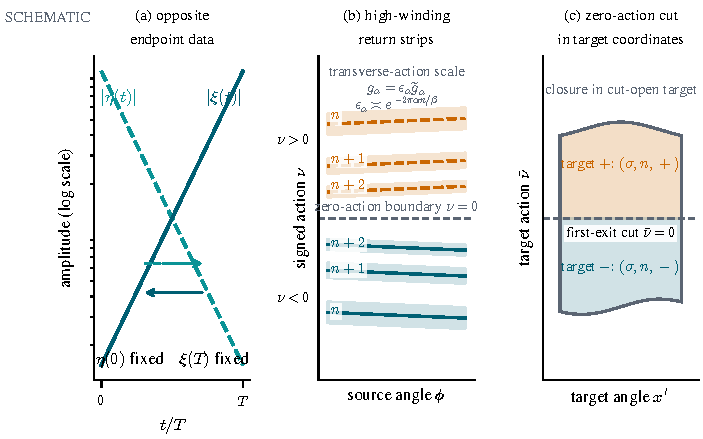
\includegraphics[width=\linewidth]{figures/signed_seam_crossform.pdf}
\caption{Opposite-endpoint boundary data and the transverse-action scale.
\textup{(a)} The stable coordinate is prescribed at $t=0$ and the unstable
coordinate at $t=T$; the curves are the leading linear decay profiles.
\textup{(b)} High-winding return strips on both sides accumulate at the
zero-action boundary on the scale
$g_a=\epsilon_a\widetilde g_a$,
$\epsilon_a\asymp e^{-2\pi\alpha n/\beta}$.
\textup{(c)} The target zero-action set cuts the closed return strip into
its two target-sign components; their common boundary
$\mathcal I_{\sigma,n}$ is a first-exit set, not a return branch.
All three panels are schematic.}
\label{fig:causal-seam}
\end{figure}

\subsection{Main results}

\begin{theorem}[Marked high-winding returns and first exits near a Hamiltonian
saddle-focus]
\label{thm:main}
Fix $k\ge5$.  Let $\mathbf X_*$ satisfy the geometric hypotheses of
Definition~\ref{def:two-ended-hypotheses}.
For every chosen exponential rate
\begin{equation}\label{eq:kappa-range}
 0<\kappa<\frac{2\pi\alpha_*}{\beta_*}
\end{equation}
there exist a relatively open neighborhood
$\cU_\kappa\subset\mathfrak H_{\mathrm{adm}}^k$ of $\mathbf X_*$, a
fixed interval $I_s$, an integer $N$, a width $\nu_N>0$, and constants
\begin{equation}\label{eq:uniform-margins}
 0<\vartheta<1,\qquad \rho_{\mathrm{in}}>0,\qquad
 \delta_{\mathrm{event}}>0,\qquad C<\infty
\end{equation}
such that the following statements hold for every
$\mathbf X\in\cU_\kappa$.

\begin{enumerate}
\renewcommand{\labelenumi}{\textup{(\roman{enumi})}}
\item \textup{\textbf{Continued geometry and the two ends.}}
The continued homoclinic and compact first-hit tubes, the algebraic
normally expanding hypersurface, and the pole sink channel exist with common coorientations,
bunching, and first-hit margins.  At the algebraic end a reference orbit
is selected at the fixed cut $e=e_*$, $E=b=0$.  Every algebraic first-exit
orbit can be compared with it at the same value of $e$; their difference
is $O(e^m)$ in $C^2$ for every fixed $m$, uniformly on the compact
algebraic entrance-label set.

\item \textup{\textbf{Complete first-return/first-exit partition.}}
The actual flow gives a disjoint and exhaustive first-return/first-exit
partition of $\Sigma_N$ into the nonempty connected return and first-exit
strata produced by the fixed cell decomposition.  These consist of
high-winding return strips, stable-manifold cut curves, and the
nonempty algebraic, pole, outgoing-boundary, and return-boundary
components.  Every disjoint union below ranges only over nonempty
connected components.  Every return or first-exit component has a unique
winding $n\ge N$ and current sign.  Every recurrent edge also has a unique
next sign; the zero set separating the two next signs is the
type-$\mathrm{cut}$ first-exit curve, not a return edge.  Finite first-exit
components have their unique cell label.  The event speeds, strict
auxiliary face-ordering inequalities, and least singular values of the
active defining-function families are bounded below by
$\delta_{\mathrm{event}}$; the labelled sign pattern is preserved.

For every source sign and every $n\ge N$, both target-sign return
components are nonempty, and their common cut-face curve
$\mathcal I_{\sigma,n}$ is nonempty; equivalently,
$\mathcal G_N=\{+,-\}^2$.  For each
$\mathsf t\in\{\mathrm a,\mathrm p\}$, the interior anchor selected in
\textup{(H2)} continues into a nonempty
$E_{\mathsf t,\sigma_{\mathsf t},n,\ell_{\mathsf t}}$ for every
$n\ge N$.  No nonemptiness is asserted for every source sign or for any
other algebraic or pole cell label.

\item \textup{\textbf{Uniform return maps.}}
In the two fixed vertex charts \eqref{eq:signed-vertex-charts} and
after pullback to the fixed rectangle $I\times[0,1]$ and fixed
first-exit reference domains, the first-return map
$P_a:V_a\to W_a$ for every edge $a=(\sigma,n,\sigma')$ has a Shilnikov
cross form (called a cross form below)
\begin{equation}\label{eq:headline-cross}
 x'=f_a(x,y'),\qquad y=g_a(x,y'),
\end{equation}
and put
\begin{equation}\label{eq:headline-seam-scale}
 \epsilon_{\mathbf X,a}
 =\nu_N^{-1}\exp\!\left(
       -\frac{2\pi\alpha_{\mathbf X}}{\beta_{\mathbf X}}n(a)\right),
 \qquad \widetilde g_a=g_a/\epsilon_{\mathbf X,a}.
\end{equation}
The cross form has contraction constant at most $\vartheta$,
$f_a(I\times[0,1])$ is at distance at least $\rho_{\mathrm{in}}$ from
$\partial I$, and
\begin{equation}\label{eq:headline-seam-margin}
 \rho_{\mathrm{in}}\le\widetilde g_a\le\rho_{\mathrm{in}}^{-1},
 \qquad g_a\le1-\rho_{\mathrm{in}},
 \qquad \|Dg_a\|_{C^1}\le C\epsilon_{\mathbf X,a}.
\end{equation}
For each fixed sign pair $(\sigma,\sigma')$ there are $C^2$ limit maps
$f_{\mathbf X,\sigma,\sigma',\infty}$ and
$\widetilde g_{\mathbf X,\sigma,\sigma',\infty}$ such that
\begin{equation}\label{eq:headline-cross-limits}
 \|f_a-f_{\mathbf X,\sigma,\sigma',\infty}\|_{C^2}
 +\|\widetilde g_a-\widetilde g_{\mathbf X,\sigma,\sigma',\infty}\|_{C^2}
 \le C(1+n)^3e^{-\kappa n}.
\end{equation}

\end{enumerate}
\end{theorem}

Figure~\ref{fig:two-end-action-finite-parts} contrasts the two finite-part
constructions and shows where exact composition enters.
\begin{figure}[t]
\centering
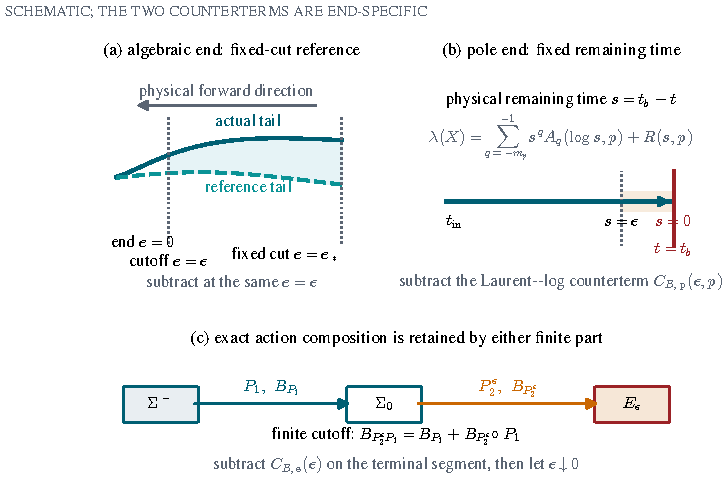
\includegraphics[width=\linewidth]{figures/two_end_action_finite_parts.pdf}
\caption{Finite parts at the two singular ends (schematic).
In both cases the renormalized action has the form
$B^{\rm ren}=\lim_{\epsilon\downarrow0}
(B^\epsilon-C_B^\epsilon)$, but the counterterm $C_B^\epsilon$ is
end-specific.
\textup{(a)} At the algebraic end, the actual and reference tails are
distinct trajectories compared at the same cutoff $e=\epsilon$ after a
fixed cut $e=e_*$; the difference of their action integrals defines the
finite part.
\textup{(b)} At the pole, the asymptotic variable is the physical remaining
time $s=t_b-t$; the end-specific Laurent--log counterterm is subtracted at
$s=\epsilon$.  \textup{(c)} Exact action composition is first used at each
finite cutoff.  The appropriate counterterm is then subtracted only from
the terminal segment before the cutoff tends to the end.  The algebraic
and pole counterterms are different objects; the diagram does not assert
that they are equal.}
\label{fig:two-end-action-finite-parts}
\end{figure}

\begin{theorem}[Renormalized time and exact action]
\label{thm:time-action}
Under the hypotheses and with the return and first-exit components of
Theorem~\ref{thm:main}, the following statements hold uniformly for
$\mathbf X\in\cU_\kappa$.
\begin{enumerate}
\renewcommand{\labelenumi}{\textup{(\roman{enumi})}}
\item \textup{\textbf{Renormalized return times and actions.}}
For an edge $a$, let
\[
 \iota_{\mathbf X,a}(x,y')=(x,g_a(x,y'))
\]
in the fixed source chart.  The physical branch time and abbreviated action
on $V_a$ are
\begin{equation}\label{eq:headline-time-action}
 \tau^{\mathrm{phys}}_{\mathbf X,a}
   =\frac{2\pi}{\beta_{\mathbf X}}n(a)
       +\widehat\tau^{\mathrm{phys}}_{\mathbf X,a},
 \qquad
 B^{\mathrm{phys}}_{\mathbf X,a}(z)=
 \int_0^{\tau^{\mathrm{phys}}_{\mathbf X,a}(z)}
    \lambda_{\mathbf X}(X_{\mathbf X})
          (\Phi_{\mathbf X}^tz)\,dt.
\end{equation}
In every $C^2$ norm and evaluation below we use the fixed-rectangle
pullbacks
$\widehat\tau_{\mathbf X,a}
 =\widehat\tau^{\mathrm{phys}}_{\mathbf X,a}\circ\iota_{\mathbf X,a}$ and
$B_{\mathbf X,a}
 =B^{\mathrm{phys}}_{\mathbf X,a}\circ\iota_{\mathbf X,a}$.
For each sign pair $(\sigma,\sigma')$ there are $C^2$ functions
$\widehat\tau_{\mathbf X,\sigma,\sigma',\infty}$ and
$B_{\mathbf X,\sigma,\sigma',\infty}$ such that every return edge with
these signs satisfies
\begin{equation}\label{eq:headline-return-potential-limits}
 \|\widehat\tau_{\mathbf X,a}
      -\widehat\tau_{\mathbf X,\sigma,\sigma',\infty}\|_{C^2}
 +\|B_{\mathbf X,a}-B_{\mathbf X,\sigma,\sigma',\infty}\|_{C^2}
 \le C(1+n)e^{-\kappa n}.
\end{equation}
For each nonempty first-exit family with type $\mathsf t$, source sign
$\sigma$, and fixed cell label $\ell$, the corresponding renormalized time
and action converge in $C^2$ to functions
$\widehat\tau^{\mathrm{ren}}_{\mathbf X,\mathsf t,\sigma,\infty,\ell}$
and $B^{\mathrm{ren}}_{\mathbf X,\mathsf t,\sigma,\infty,\ell}$, with
error at most $C(1+n)^3e^{-\kappa n}$.  The algebraic branch uses fixed-cut
reference counterterms for time and action.  Pole flight time is already
finite and uses zero end counterterm; only the pole action uses the
physical-remaining-time Laurent--log counterterm.  Finite lateral and
cut-face events have zero end counterterm.

\item \textup{\textbf{Exact branch primitives.}}
On every finite branch, writing $\Sigma_a^-$ and $\Sigma_a^+$ for
its marked source and target sections,
\begin{equation}\label{eq:headline-exact}
 P_a^*(\lambda_{\mathbf X}|_{\Sigma_a^+})
  -\lambda_{\mathbf X}|_{\Sigma_a^-}
 =d_{\Sigma_a^-}B^{\mathrm{phys}}_{\mathbf X,a}.
\end{equation}
Composition is exact because the same orbit integral is split at
intermediate sections.  Orbit-following section changes and exact changes
of primitive satisfying Proposition~\ref{prop:section-gauge-covariance}
alter the renormalized actions only by endpoint coboundaries.

\end{enumerate}
\end{theorem}

\begin{theorem}[Coding and parameter dependence]
\label{thm:coding-persistence}
Under the hypotheses and with the objects of Theorems~\ref{thm:main} and
\ref{thm:time-action}, the following statements hold.
\begin{enumerate}
\renewcommand{\labelenumi}{\textup{(\roman{enumi})}}
\item \textup{\textbf{Countable Markov coding.}}
The return graph has the two vertices $\Sigma_+$ and $\Sigma_-$ and all edges
$a=(\sigma,n,\sigma')$ with source $\sigma$ and target $\sigma'$.
Let $\Sigma_{\mathcal G_N}$ be its two-sided edge shift, and let
$K_{\mathbf X}\subset\Sigma_N$ be the set on which the first-return map is
defined for all positive and negative iterates.  The map
$h_{\mathbf X}:\Sigma_{\mathcal G_N}\to K_{\mathbf X}$ is a homeomorphism
for the product-discrete topology.  Every one-sided infinite future word
determines a stable plaque; every point outside the forward trapped set has
a finite return word followed by a unique first-exit component.  For each
source sign, the closures of the uncut return strips in the cut-open section
form a Hausdorff compact alphabet; the edge alphabet is its finite discrete
next-sign extension.  First-exit labels remain discrete and are not
compactified.  The renormalized roof and action on recurrent codes have
summable variations.

\item \textup{\textbf{Persistence and parameter dependence.}}
The construction is continuous from $\cU_\kappa$ to a fixed weighted
$C^2$ space of return and first-exit data.  Let $\mathcal P$ be a compact
finite-dimensional parameter manifold, let $r\in\{1,2\}$, and let
\[
 \mathcal P\longrightarrow\cU_\kappa,
 \qquad \varpi\longmapsto\mathbf X_\varpi,
\]
be a $C^r$ map whose image is compact in the coefficient topology of
Definition~\ref{def:field-space}.  The state-only geometric constants work
uniformly on its image.  The return and compact first-hit maps, the
recurrent time/action data, and both renormalized end limits have all mixed
derivatives $D_z^iD_\varpi^j$, $i+j\le2$, $j\le r$, with the same
$e^{-\kappa n}$ weights.  The multiplicative constants for derivatives
with $j>0$ may depend on the $C^r$ coefficient norm of the chosen
parameterization.  The same mixed two-jet statement applies to the
same-$e$ algebraic comparison in Theorem~\ref{thm:main}\textup{(i)}.  At
the pole the finite jets may vary subject to the
$C^{m_{\mathrm p}+3}$ family condition
\eqref{eq:pole-parameter-class};
Proposition~\ref{prop:pole-varying-jet-finite-part} extracts every
nonintegrable Laurent--log term with the same mixed regularity.

\end{enumerate}
\end{theorem}

\begin{proof}[Proof of Theorem~\ref{thm:main-result}]
Apply Theorem~\ref{thm:local-chart-production}.  After a finite refinement
of \eqref{eq:finite-parameter-chart-cover}, the compact image of every
$\overline V_i$ is covered by finitely many coefficient neighborhoods on
which Theorems~\ref{thm:main}--\ref{thm:coding-persistence} apply.  The
chosen inequality for $\kappa$ leaves a strict rate gap on all of them.
Take the maximum of their marked winding thresholds and all finite
first-event thresholds.  The interior margins in the physical source cell
allow one smaller physical source collar to be used throughout the finite
cover.

Theorem~\ref{thm:main}\textup{(i)--(ii)} gives the exhaustive marked
return/first-event partition, including the two selected nonempty end
families, and its part~\textup{(iii)} gives the cross forms.
Theorem~\ref{thm:time-action} gives the time, end finite-part, and exact
action statements.  Theorem~\ref{thm:coding-persistence}\textup{(i)} gives
the local coding and summable variations.

Now use \eqref{eq:physical-tail-implies-local-tail} to choose $T_*$ above
every marked threshold.  The marked partitions therefore restrict to an
exhaustive physical relation on the part of the smaller source collar whose
saddle-block residence time is at least $T_*$.  On overlaps,
Theorem~\ref{thm:change-of-marking} identifies that relation, the trapped
Poincar\'e system, and the corrected weighted data after a finite clean
refinement.  Its deck and endpoint-coboundary formulas preserve closed
periods and closed actions.  This proves all four parts, including the
stated limitation on global symbolic labels.
\end{proof}

\begin{corollary}[Descent from a finite marked atlas]
\label{cor:physical-covariance}
Let $\mathcal P$ be compact, $r\in\{0,1,2\}$, and consider a $C^r$
family of physical reversible exact Hamiltonian return--exit tubes.
Suppose a finite cover $\mathcal P=\bigcup_iV_i$ carries $C^r$ marked
representations
\[
 p\longmapsto\mathbf X_{i,p}\in\mathfrak H_{\mathrm{adm}}^k
\]
with compact local images to which
Theorems~\ref{thm:main}--\ref{thm:coding-persistence} apply.  Suppose that
on every overlap the representations describe the same physical event
hypersurfaces and are admissibly related in the sense of
Definition~\ref{def:compatible-marking-change}.  Then, after increasing
the finitely many local winding thresholds, the following statements hold.
\begin{enumerate}
\renewcommand{\labelenumi}{\textup{(\roman{enumi})}}
\item The local exhaustive return/first-exit partitions descend to one
physical first-event relation.  The Poincar\'e-conjugacy class of its
trapped return system, the periods of its closed orbits, and their actions
for the fixed primitive are independent of the representation.
\item The corrected return maps, roof and action functions, first-exit
data, and the two renormalized end limits form the compatible family of
weighted mixed-$C^2$ data defined by
Theorem~\ref{thm:change-of-marking}.  Raw winding labels, individual limit
maps, references, and end counterterms remain local representatives.
\item Each marking has its local full countable edge shift.  When two cuts
cross, the two codings compare through the realized-itinerary factor on a
finite common refinement; a global labeled full shift is not inferred.
Event-preserving section slides and exact gauges change roof and action
only by the endpoint coboundaries in
Proposition~\ref{prop:section-gauge-covariance}.  Closed periods and closed
exact-gauge actions are unchanged.
\end{enumerate}
A single global marked lift is the special case of a one-chart atlas; it is
not required.
\end{corollary}

\begin{corollary}[High-winding period, action, and first-exit asymptotics]
\label{cor:period-action-asymptotics}
Fix $\mathbf X\in\cU_\kappa$ and a cyclic sign sequence
$\boldsymbol\sigma=(\sigma_0,\ldots,\sigma_m)$, $m\ge1$, with
$\sigma_m=\sigma_0$.  For
$\mathbf n=(n_0,\ldots,n_{m-1})$, $n_j\ge N$, put
\begin{equation}\label{eq:periodic-error-scale}
 a_j=(\sigma_j,n_j,\sigma_{j+1}),\qquad
 \Delta_\kappa(\mathbf n)
 =\max_{0\le j<m}(1+n_j)^3e^{-\kappa n_j}.
\end{equation}
Assume that the cyclic edge word $a_0\cdots a_{m-1}$ is primitive.  Its
repetition codes a unique periodic orbit $\gamma_{\mathbf n}$ with exactly
$m$ first returns.  A nonprimitive word is covered by applying the statement
to its primitive cyclic subword.

Let $(x_j^\infty)_{j\in\mathbb Z/m\mathbb Z}$ be the unique solution of
\begin{equation}\label{eq:limiting-cyclic-cross-form}
 x_{j+1}^\infty
 =f_{\mathbf X,\sigma_j,\sigma_{j+1},\infty}
       (x_j^\infty,0).
\end{equation}
Define
\begin{align}
 \mathcal T_{\boldsymbol\sigma,\mathbf X}
 &=\sum_{j=0}^{m-1}
   \widehat\tau_{\mathbf X,\sigma_j,\sigma_{j+1},\infty}
       (x_j^\infty,0),\label{eq:limiting-period-constant}\\
 \mathcal A_{\boldsymbol\sigma,\mathbf X}
 &=\sum_{j=0}^{m-1}
   B_{\mathbf X,\sigma_j,\sigma_{j+1},\infty}
       (x_j^\infty,0).
 \label{eq:limiting-action-constant}
\end{align}
Then, as $\min_jn_j\to\infty$,
\begin{align}
 \operatorname{per}(\gamma_{\mathbf n})
 &=\frac{2\pi}{\beta_{\mathbf X}}\sum_{j=0}^{m-1}n_j
   +\mathcal T_{\boldsymbol\sigma,\mathbf X}
   +O\bigl(\Delta_\kappa(\mathbf n)\bigr),
 \label{eq:period-asymptotic}\\
 \oint_{\gamma_{\mathbf n}}\lambda_{\mathbf X}
 &=\mathcal A_{\boldsymbol\sigma,\mathbf X}
   +O\bigl(\Delta_\kappa(\mathbf n)\bigr).
 \label{eq:action-asymptotic}
\end{align}

There is an analogous $C^2$ statement for first exits.  Fix a finite sign
path $\sigma_0,\ldots,\sigma_m$, a first-exit type $\mathsf t$, and a cell
label $\ell$.  Restrict to winding vectors for which the full finite
cylinder consisting of the prescribed return branches followed by that
first-exit component is nonempty, and identify these cylinders by the fixed
component chart.  For return windings $n_0,\ldots,n_{m-1}$ and final
winding $n_m$, set $a_j=(\sigma_j,n_j,\sigma_{j+1})$ for $j<m$ and define,
with every term evaluated along the corresponding finite composition,
\begin{align*}
 \tau_{\mathbf n}^{\rm end}
 &=\sum_{j=0}^{m-1}\left(
     \frac{2\pi}{\beta_{\mathbf X}}n_j+\widehat\tau_{a_j}\right)
   +\frac{2\pi}{\beta_{\mathbf X}}n_m
   +\widehat\tau^{\mathrm{ren}}_{\mathsf t,\sigma_m,n_m,\ell},\\
 B_{\mathbf n}^{\rm end}
 &=\sum_{j=0}^{m-1}B_{a_j}
   +B^{\mathrm{ren}}_{\mathsf t,\sigma_m,n_m,\ell}.
\end{align*}
Here the final renormalized terms are those of
\eqref{eq:terminal-potentials-time}--\eqref{eq:terminal-potentials}.  At the
algebraic end they are defined by a cutoff limit after subtraction of the
end counterterm, never by subtracting two infinite quantities; the pole
action is understood in the same cutoff-renormalized sense.  On the fixed
component chart there are
$C^2$ limit functions
$\mathcal T^{\rm exit}_{\boldsymbol\sigma,\mathsf t,\ell,\mathbf X}$ and
$\mathcal A^{\rm exit}_{\boldsymbol\sigma,\mathsf t,\ell,\mathbf X}$ such
that
\begin{align}
 &\left\|\tau_{\mathbf n}^{\rm end}
   -\frac{2\pi}{\beta_{\mathbf X}}\sum_{j=0}^{m}n_j
   -\mathcal T^{\rm exit}_{\boldsymbol\sigma,\mathsf t,\ell,\mathbf X}
   \right\|_{C^2}\notag\\
 &\qquad+
 \left\|B_{\mathbf n}^{\rm end}
   -\mathcal A^{\rm exit}_{\boldsymbol\sigma,\mathsf t,\ell,\mathbf X}
   \right\|_{C^2}
 \le C\max_{0\le j\le m}(1+n_j)^3e^{-\kappa n_j}.
 \label{eq:first-exit-time-action-asymptotic}
\end{align}
The two limit functions are the sums of the limiting return functions and
the limiting first-exit function along the corresponding limiting
composition.

The complete period and action asymptotics are unchanged under the section
slides and exact gauges in
Proposition~\ref{prop:section-gauge-covariance}.  The individual constants
in \eqref{eq:limiting-period-constant}--
\eqref{eq:limiting-action-constant} use the fixed winding and endpoint
normalizations; their transformation laws are
\eqref{eq:roof-section-coboundary}--
\eqref{eq:winding-change-covariance}.
\end{corollary}

\begin{proof}[Proof of Corollary~\ref{cor:period-action-asymptotics}]
On the cyclic product of $m$ section rectangles, the cross-form equations
define a contraction with constant at most $\vartheta$.  By
\eqref{eq:headline-seam-scale}--\eqref{eq:headline-cross-limits}, this
contraction differs from the
limiting contraction in \eqref{eq:limiting-cyclic-cross-form} by
$O(\Delta_\kappa(\mathbf n))$.  The inverse bound
$(1-\vartheta)^{-1}$ therefore gives the same estimate for their fixed
points.  Substitution into \eqref{eq:headline-return-potential-limits} and
summation over the fixed number $m$ of branches proves
\eqref{eq:period-asymptotic}--\eqref{eq:action-asymptotic}.  The period is
the sum of the actual branch flight times, and
\eqref{eq:action-composition} identifies the action sum with the closed
orbit integral.  Injectivity of the coding identifies the fixed point with
the periodic orbit of the primitive word.

On a nonempty fixed finite cylinder ending in a first exit, the same argument
is a finite induction through the return maps, followed by the $C^2$ first-exit
limit in Theorem~\ref{thm:time-action}.  This gives
\eqref{eq:first-exit-time-action-asymptotic}.  Section and primitive changes
contribute endpoint coboundaries.  They telescope on a periodic word; for a
first-exit path they are the endpoint terms fixed by the chosen normalization.
\end{proof}

For a quantitative dynamical consequence, discard every return whose
winding is smaller than a second threshold $L\ge N$.  The resulting
subsystem is still countable: from either signed section there is one edge
of winding $n$ to each signed section for every $n\ge L$.  Completeness of
the return--exit partition is important here.  It identifies all trapped
orbits satisfying this winding restriction, rather than only a subshift
chosen inside the return map.

\begin{theorem}[Entropy and action of the high-winding trapped sets]
\label{thm:tail-entropy-action}
Fix $\mathbf X\in\cU_\kappa$ and put
\begin{equation}\label{eq:tail-roof-slope}
 c_{\mathbf X}=\frac{2\pi}{\beta_{\mathbf X}}.
\end{equation}
For $L\ge N$, let
\begin{equation}\label{eq:tail-shift}
 \Sigma_L=\{\omega\in\Sigma_{\mathcal G_N}:
       n(\omega_j)\ge L\text{ for every }j\in\mathbb Z\},
\end{equation}
and let $\Lambda_L$ be the corresponding suspension of the trapped
Poincar\'e system inside the fixed flow tube.  On $\Sigma_L$ denote the
physical roof and branch action by
\begin{align}
 r_{\mathbf X}(\omega)
 &=\tau^{\mathrm{phys}}_{\mathbf X,\omega_0}
       (h_{\mathbf X}(\omega)),\label{eq:tail-roof}\\
 b_{\mathbf X}(\omega)
 &=B^{\mathrm{phys}}_{\mathbf X,\omega_0}
       (h_{\mathbf X}(\omega)).\label{eq:tail-action}
\end{align}
There are constants $M_\tau,M_B<\infty$, independent of $L$, such that
\begin{equation}\label{eq:tail-potential-bounds}
 |r_{\mathbf X}(\omega)-c_{\mathbf X}n(\omega_0)|\le M_\tau,
 \qquad |b_{\mathbf X}(\omega)|\le M_B.
\end{equation}
In the pressure notation below,
$P_{\Sigma_L}(-s r_{\mathbf X})$ means the pressure of the cohomologous
one-sided representative $r_{\mathbf X}^+$ supplied by
Lemma~\ref{lem:tail-thermodynamic-hypotheses}; bounded cohomology makes
this choice immaterial.

For all sufficiently large $L$, the equation
\begin{equation}\label{eq:tail-pressure-root}
 P_{\Sigma_L}(-s r_{\mathbf X})=0
\end{equation}
for Gurevich pressure has a unique positive root $h_L(\mathbf X)$.  This
root is the variational entropy of the suspension flow on $\Lambda_L$, and
\begin{equation}\label{eq:tail-entropy-asymptotic}
 h_L(\mathbf X)
 =\frac{1}{c_{\mathbf X}L}
   \left\{W(2L)+O\!\left(\frac{W(L)}{L}\right)\right\},
\end{equation}
where $W$ is the principal branch of the Lambert $W$-function.  Equivalently,
\begin{equation}\label{eq:tail-entropy-log-asymptotic}
 h_L(\mathbf X)
 =\frac{\beta_{\mathbf X}}{2\pi L}
   \bigl(\log L-\log\log L+\log2+o(1)\bigr).
\end{equation}
The error estimates are uniform when $\mathbf X$ ranges over a compact
subset of $\cU_\kappa$.

Every periodic orbit $\gamma\subset\Lambda_L$ satisfies
\begin{equation}\label{eq:tail-periodic-action-rate}
 \frac{\left|\displaystyle\oint_\gamma\lambda_{\mathbf X}\right|}
      {\operatorname{per}(\gamma)}
 \le \frac{M_B}{c_{\mathbf X}L-M_\tau}=O(L^{-1}).
\end{equation}
More generally, if $\mu$ is a shift-invariant probability measure on
$\Sigma_L$ and $\int r_{\mathbf X}\,d\mu<\infty$, then
\begin{equation}\label{eq:tail-measure-action-rate}
 \frac{\left|\int b_{\mathbf X}\,d\mu\right|}
      {\int r_{\mathbf X}\,d\mu}
 \le \frac{M_B}{c_{\mathbf X}L-M_\tau}.
\end{equation}
Thus the entropy of the complete high-winding tail has the explicit scale
$(\log L)/L$, while its action per unit physical time tends uniformly to
zero.
\end{theorem}

\begin{lemma}[Thermodynamic hypotheses for the high-winding tail]
\label{lem:tail-thermodynamic-hypotheses}
For all sufficiently large $L$, the one-sided presentation of
$\Sigma_L$ is a topologically mixing countable Markov shift, and the
following facts hold.
\begin{enumerate}
\renewcommand{\labelenumi}{\textup{(\roman{enumi})}}
\item There are bounded transfer functions, with bounds independent of
$L$, which replace $r_{\mathbf X}$ and $b_{\mathbf X}$ by cohomologous
one-sided functions $r_{\mathbf X}^+$ and $b_{\mathbf X}^+$.  These
functions have summable variations and
\begin{equation}\label{eq:tail-one-sided-roof-bounds}
 r_{\mathbf X}^+\ge c_{\mathbf X}L-C_\tau>0,
 \qquad
 |r_{\mathbf X}^+-c_{\mathbf X}n(\omega_0)|\le C_\tau
\end{equation}
for a constant $C_\tau$ independent of $L$.
\item For every $s>0$, the Gurevich pressure
$P_{\Sigma_L}(-s r_{\mathbf X}^+)$ is finite.  It is continuous and
strictly decreasing in $s$, tends to $+\infty$ as $s\downarrow0$, and
tends to $-\infty$ as $s\to\infty$.
\item The suspension variational principle applies and gives
\begin{equation}\label{eq:tail-suspension-variational-principle}
 h_{\rm var}(\Lambda_L)=
 \sup_{\substack{\mu\ \mathrm{shift\text{-}invariant}\\
                  \int r_{\mathbf X}^+\,d\mu<\infty}}
\frac{h_\mu(\sigma)}{\int r_{\mathbf X}^+\,d\mu}.
\end{equation}
Here $h_{\rm var}$ denotes the supremum of metric entropies over invariant
probability measures of the suspension flow.
No positive-recurrence assumption is needed for this assertion: it is a
statement about the supremum and the pressure zero, not about existence of
a maximizing probability measure.
\end{enumerate}
\end{lemma}

\begin{proof}[Proof of Lemma~\ref{lem:tail-thermodynamic-hypotheses}]
The full two-vertex incidence, including self-edges of every winding,
makes the one-sided shift topologically mixing.  The exponential
two-sided variation estimates from
Theorem~\ref{thm:coding-persistence} give the usual telescoping
two-sided-to-one-sided cohomology construction.  Its transfer functions
are bounded by the sum of a geometric series, uniformly after symbols with
winding below $L$ are discarded.  Together with
\eqref{eq:tail-potential-bounds}, this proves summable variations and
\eqref{eq:tail-one-sided-roof-bounds} after increasing $L$.

For $r_0(\omega)=c_{\mathbf X}n(\omega_0)$, the weighted transition matrix
has spectral radius
\[
 2\sum_{n=L}^{\infty}e^{-s c_{\mathbf X}n}
 =2\frac{e^{-s c_{\mathbf X}L}}{1-e^{-s c_{\mathbf X}}}.
\]
The bounded difference between $r_{\mathbf X}^+$ and $r_0$ changes
pressure by at most $sC_\tau$.  Hence pressure is finite for $s>0$ and
has the stated endpoint limits.  The positive lower roof bound makes it
strictly decreasing; convexity makes it continuous.  Finally, the
variational principle for finite-pressure summable-variation potentials,
followed by the suspension variational principle and Abramov's formula,
gives \eqref{eq:tail-suspension-variational-principle}
\cite{Sarig1999Thermodynamic,BarreiraIommi2006Suspension}.  These results
identify the supremum without requiring an equilibrium measure.
\end{proof}

\begin{proof}[Proof of Theorem~\ref{thm:tail-entropy-action}]
Theorem~\ref{thm:time-action} first gives
\eqref{eq:tail-potential-bounds}.  Apply
Lemma~\ref{lem:tail-thermodynamic-hypotheses} and use its one-sided
representatives below; bounded cohomology preserves pressure, periodic
sums, invariant-measure integrals, and the suspension up to a change of
section.  Increase $M_\tau$, if necessary, so that
$\|r_{\mathbf X}^+-r_0\|_\infty\le M_\tau$.

We use the convention that $P_{\Sigma_L}$ denotes Gurevich pressure for
the one-sided presentation of the shift.  First replace the roof by the one-coordinate function
$r_0(\omega)=c_{\mathbf X}n(\omega_0)$.  The weighted transition matrix
between the two signed vertices has all four entries equal to
\begin{equation}\label{eq:tail-geometric-series}
 R_L(s)=\sum_{n=L}^\infty e^{-s c_{\mathbf X}n}
       =\frac{e^{-s c_{\mathbf X}L}}
              {1-e^{-s c_{\mathbf X}}}.
\end{equation}
Its spectral radius is $2R_L(s)$, and hence
\begin{equation}\label{eq:tail-model-pressure}
 P_{\Sigma_L}(-s r_0)
 =\log\!\left(
       2\frac{e^{-s c_{\mathbf X}L}}
               {1-e^{-s c_{\mathbf X}}}\right).
\end{equation}
Since Gurevich pressure changes by at most the uniform norm of a potential,
the preceding one-sided bound gives
\begin{equation}\label{eq:tail-pressure-comparison}
 P_{\Sigma_L}(-s r_0)-sM_\tau
 \le P_{\Sigma_L}(-s r_{\mathbf X}^+)
 \le P_{\Sigma_L}(-s r_0)+sM_\tau.
\end{equation}
Lemma~\ref{lem:tail-thermodynamic-hypotheses} proves existence and
uniqueness of the pressure zero and identifies it with
\begin{equation}\label{eq:tail-variational-entropy}
 h_L(\mathbf X)=
 \sup_{\substack{\mu\ \text{a shift-invariant probability measure}\\
                  \int r_{\mathbf X}\,d\mu<\infty}}
 \frac{h_\mu(\sigma)}{\int r_{\mathbf X}\,d\mu}
\end{equation}.

Set $x=c_{\mathbf X}Lh_L$.  Before expanding the denominator in
\eqref{eq:tail-model-pressure}, note that $x\to\infty$ and $x/L\to0$.
Indeed, bounded $x$ would
make the model pressure grow like $\log L$, contrary to
$|P_{\Sigma_L}(-h_Lr_0)|\le h_LM_\tau$; while $x/L$ bounded away from zero
would make its negative linear term dominate the same right-hand side.
Using $s=h_L$ in
\eqref{eq:tail-model-pressure}--\eqref{eq:tail-pressure-comparison} together
with the expansion $1-e^{-x/L}=(x/L)(1+O(x/L))$ gives
\begin{equation}\label{eq:tail-lambert-equation}
 x+\log x=\log(2L)+O(x/L).
\end{equation}
The inverse of $x\mapsto x+\log x$ is $W(e^{(\cdot)})$ and has derivative
$x/(1+x)$.  Hence
\[
 x=W(2L)+O(W(L)/L),
\]
which proves \eqref{eq:tail-entropy-asymptotic}.  The standard expansion of
$W$ gives \eqref{eq:tail-entropy-log-asymptotic}.  The constants used in
the comparison are uniform on compact field families, proving the uniform
version.

If a periodic code has $m$ returns, exact action composition and
\eqref{eq:tail-potential-bounds} give
\[
 \left|\oint_\gamma\lambda_{\mathbf X}\right|\le mM_B,
 \qquad
 \operatorname{per}(\gamma)\ge m(c_{\mathbf X}L-M_\tau).
\]
This proves \eqref{eq:tail-periodic-action-rate}.  Integrating the same
pointwise inequalities proves \eqref{eq:tail-measure-action-rate}.
\end{proof}

\begin{remark}[Physical conclusions and auxiliary choices]
The first-return/first-exit partition is defined by the physical flow in
the fixed flow tube, and moving an intermediate section along that flow
gives the Poincar\'e conjugacy and endpoint coboundaries proved in
Proposition~\ref{prop:section-gauge-covariance}.  Periods are independent
of coordinates.  For the fixed primitive, $\oint\lambda_{\mathbf X}$ is
also coordinate-independent and is unchanged by an exact gauge
$\lambda\mapsto\lambda+d\chi$; it need not be unchanged after adding a
non-exact closed one-form.  The integer winding labels, individual limiting
cross forms, and chosen algebraic reference do change with the chosen
presentation.  Under the admissibility conditions of
Definition~\ref{def:compatible-marking-change},
Theorem~\ref{thm:change-of-marking} gives their exact deck, coboundary, and
end-correction laws and proves that, after a common finite refinement, the
metric overlap maps are locally bi-Lipschitz.  Thus the topology defined by
these overlaps, rather than any one labeled representative, is intrinsic.
\end{remark}

The following selected-branch consequence is an optional module.  It is not
used in the return--exit theorem, its RFSN-II realization, or the coding and
action conclusions.

\begin{corollary}[Optional module: critical points on a selected reversible branch]
\label{cor:source-fold-persistence}
Assume, in addition to the hypotheses of Theorem~\ref{thm:main}, that the
algebraic entrance hypersurface $\mathcal W_{\mathrm a,*}$ contains a
selected critical-energy connection
\[
 \Gamma_{\mathrm a,*}\subset
 W^u(O_*)\cap\mathcal W_{\mathrm a,*}\cap H_*^{-1}(0),
\]
and that the two invariant manifolds meet transversely modulo their common
flow direction.  Equivalently, at one, hence every, regular point
$q_*\in\Gamma_{\mathrm a,*}$,
\[
 T_{q_*}W^u(O_*)+T_{q_*}\mathcal W_{\mathrm a,*}=T_{q_*}M,
 \qquad
 T_{q_*}W^u(O_*)\cap T_{q_*}\mathcal W_{\mathrm a,*}
 =\operatorname{span}\{X_*(q_*)\}.
\]
Then the neighborhood $\cU_\kappa$ in Theorem~\ref{thm:main} may be
decreased so that the following holds for every
$\mathbf X\in\cU_\kappa$.  Denote by
$\Gamma_{\mathrm a,\mathbf X}$ the transverse continuation of
$\Gamma_{\mathrm a,*}$ and by $\mathcal W_{\mathrm a,\mathbf X}$ the
continued algebraic entrance hypersurface.
On the fixed-point plane of the reverser, let $(r,\theta)$ be local polar
coordinates defined by $\xi=\eta=rq(\theta)$, and denote by
$\gamma_{\mathbf X}^{\mathrm a}(r)$ the corresponding local branch
selected by $\Gamma_{\mathrm a,\mathbf X}$.
Its lifted angle satisfies
\begin{equation}\label{eq:source-spiral}
 \theta_{\mathbf X}(r)
 -\frac{\beta_{\mathbf X}}{\alpha_{\mathbf X}}\log r
 =\theta_{\mathbf X}^*+O_{C^2_{\log r}}(r^\eta)
\end{equation}
for one uniform $\eta>0$.  All sufficiently small critical points of
$H_{\mathbf X}$ restricted to this branch are nondegenerate, and they
alternate between maxima and minima.  The radii of consecutive critical
points satisfy
\begin{equation}\label{eq:fold-ratio}
 \frac{r_{m+1}(\mathbf X)}{r_m(\mathbf X)}
 =\exp\!\left(-\frac{\pi\alpha_{\mathbf X}}
                       {2\beta_{\mathbf X}}\right)
     \bigl(1+O(r_m(\mathbf X)^\eta)\bigr).
\end{equation}
These are critical points of the scalar function
$r\mapsto H_{\mathbf X}(\gamma_{\mathbf X}^{\mathrm a}(r))$, not zeros
of $H$.
\end{corollary}

Figure~\ref{fig:source-fold} illustrates the leading logarithmic-spiral
calculation and distinguishes the normal-form plot from the general
ratio in \eqref{eq:fold-ratio}.
\begin{figure}[t]
\centering
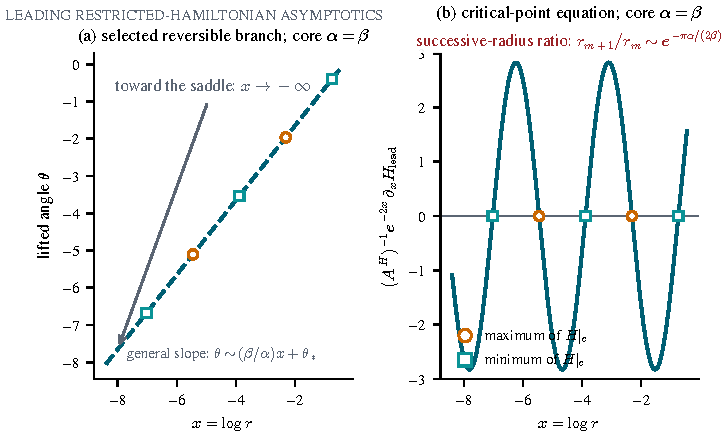
\includegraphics[width=\textwidth]{figures/spiral_fold_mechanism.pdf}
\caption{Leading-order logarithmic-spiral mechanism on the selected
reversible-plane branch.  The curves are plotted for the normal-form system
$\alpha=\beta$; the displayed formulas give the general slope
$\theta\sim(\beta/\alpha)\log r+\theta_*$ and the general ratio
$r_{m+1}/r_m\sim\exp[-\pi\alpha/(2\beta)]$.  Open circles and open squares
denote, respectively, maxima and minima of the leading restriction of
$H$.  These are critical points of the scalar restriction, not zeros of
$H$.  The diagram is asymptotic and does not provide a rigorous enclosure
of the finite continuation.}
\label{fig:source-fold}
\end{figure}

The order of quantifiers in Theorem~\ref{thm:main} is essential: the
neighborhood $\cU_\kappa$ and the threshold $N$ are chosen after fixing the
chosen rate $\kappa$.  We do not assert one neighborhood that works
uniformly as $\kappa\uparrow2\pi\alpha_*/\beta_*$.  For the normal-form
system \eqref{eq:core-intro}, this endpoint is $2\pi$.

\begin{remark}[Relative openness and the pole type]
The perturbation conclusions are open in the marked coefficient topology of
Definition~\ref{def:field-space}, not in an unrestricted compact-open
$C^k$ topology.  Condition \eqref{eq:pole-principal-class} fixes the
compactified-action order $m_{\mathrm p}$, the principal radial scaling,
and a simple positive-integer indicial spectrum, but not the finite pole
jet or the leading compactified action coefficient.  The
latter may vary and are handled by
Proposition~\ref{prop:pole-varying-jet-finite-part}.  Allowing the indicial
roots themselves to move or cross an integral resonance would require
parameter-dependent powers and uniform divided-difference coordinates;
that is outside the theorem.
\end{remark}

\section{Long saddle-focus passages and recurrent strips}
\label{sec:passage}

\subsection{Mixed boundary-value problem in Volterra form}

The axis identities \eqref{eq:axis-vanishing} imply by the double Hadamard
lemma that, in a smaller bidisk,
\begin{equation}\label{eq:double-hadamard}
 |F(\xi,\eta)|+|G(\xi,\eta)|\le C|\xi|\,|\eta|.
\end{equation}
For $T>0$ prescribe the mixed boundary conditions
\begin{equation}\label{eq:mixed-boundary}
 \eta(0)=\eta_-,\qquad \xi(T)=\xi_+,
 \qquad |\eta_-|=|\xi_+|=\delta.
\end{equation}
For the parameter statement below, let $\mathcal P$ be compact, assume
$\varpi\mapsto(A_\varpi,F_\varpi,G_\varpi)$ is $C^2$ in the preceding
coefficient norms, and require the four axis identities in
\eqref{eq:axis-vanishing} for every $\varpi\in\mathcal P$.  The boundary
vectors are parametrized by finitely many fixed $C^2$ charts.  Put
\begin{equation}\label{eq:common-passage-rate}
 \underline\alpha=\inf_{\varpi\in\mathcal P}\alpha_\varpi,
 \qquad 0<\alpha_*<\underline\alpha.
\end{equation}
At a fixed $\varpi$ we abbreviate $A=A_\varpi$ and
$\alpha=\alpha_\varpi$ in the formulas below.

\begin{lemma}[Uniform mixed passage]\label{lem:mixed-passage}
After decreasing $\delta$, for every $T\ge T_0$ and every boundary pair
in \eqref{eq:mixed-boundary} there is a unique solution in the class
\begin{equation}\label{eq:mixed-class}
 |\xi(t)|\le2\delta e^{-\alpha(T-t)},\qquad
 |\eta(t)|\le2\delta e^{-\alpha t}.
\end{equation}
It has the form
\begin{equation}\label{eq:mixed-expansion}
 \xi(t)=e^{A(t-T)}\xi_++R_\xi(t),\qquad
 \eta(t)=e^{-At}\eta_-+R_\eta(t),
\end{equation}
where
\begin{equation}\label{eq:mixed-error}
 \sup_{0\le t\le T}(|R_\xi(t)|+|R_\eta(t)|)
 \le C\delta^2e^{-\alpha T}.
\end{equation}
The same estimate holds through two boundary derivatives at fixed $T$.
With $t=Tu$ and every boundary, $T$, and field-parameter multi-index
$\gamma$ of total order at most two, where $T$ differentiation is taken at
fixed $u$,
\begin{equation}\label{eq:mixed-interior-jets}
 \sup_{0\le u\le1}
 \left|D_{(\mathrm{bdry},T,\varpi)}^\gamma
   \bigl(R_\xi(Tu),R_\eta(Tu)\bigr)\right|
 \le C_\gamma(1+T)^2e^{-\alpha_*T}.
\end{equation}
For every fixed $\alpha_*<\underline\alpha$ the two remote traces
satisfy, for every mixed multi-index of total order at most two,
\begin{equation}\label{eq:mixed-trace-jets}
 \left|D_{\rm bdry}^iD_{(T,\varpi)}^j
   \bigl(R_\xi(0),R_\eta(T)\bigr)\right|
 \le C_{ij}(1+T)^{2j+i}e^{-\alpha_*T},
 \qquad i+j\le2.
\end{equation}
The corresponding estimate for action applies to the \emph{renormalized
gluing remainder} in Lemma~\ref{lem:action-gluing}, not to the raw moving
integral.  Thus the present claim concerns endpoint traces, not an
undefined $T$ derivative of a function living on $[0,T]$.
\end{lemma}

\begin{proof}
The mixed problem is equivalent to Volterra integral equations with data
imposed at opposite endpoints:
\begin{align}
 \xi(t)&=e^{A(t-T)}\xi_+
   -\int_t^T e^{A(t-s)}F(\xi(s),\eta(s))\,ds,\label{eq:volterra-xi}\\
 \eta(t)&=e^{-At}\eta_-
   +\int_0^t e^{-A(t-s)}G(\xi(s),\eta(s))\,ds.
   \label{eq:volterra-eta}
\end{align}
For existence at a fixed $T$, the usual endpoint-weighted norm makes the
right-hand side a contraction: the double Hadamard factorization gives
$|F|+|G|\le C|\xi||\eta|$, hence the nonlinear source is
$O(\delta^2e^{-\alpha T})$ at every time.  The two Volterra kernels have
uniformly bounded $L^1$ norms, and the Lipschitz constant is $C\delta$.
After decreasing $\delta$, the contraction constant is some
$\vartheta<1$, independent of $T$ and of $\varpi\in\mathcal P$.  This
proves existence, uniqueness, \eqref{eq:mixed-class}, and
\eqref{eq:mixed-error}.

It remains to justify derivatives with respect to a moving interval.  Put
$t=Tu$ and work on the single Banach space
\begin{equation}\label{eq:volterra-norm}
 \mathcal E=C([0,1];\R^2\times\R^2),\qquad
 \|z\|_{\mathcal E}=\max_{0\le u\le1}
       \max\{|z_\xi(u)|,|z_\eta(u)|\}.
\end{equation}
Define
\begin{equation}\label{eq:fixed-domain-variables}
 \widehat\xi(u)=e^{\alpha_*T(1-u)}\xi(Tu),\qquad
 \widehat\eta(u)=e^{\alpha_*Tu}\eta(Tu).
\end{equation}
For the next display abbreviate
\[
 \xi_T(v)=e^{-\alpha_*T(1-v)}\widehat\xi(v),\qquad
 \eta_T(v)=e^{-\alpha_*Tv}\widehat\eta(v).
\]
In these variables the fixed-point map on $\mathcal E$ is
\begin{align}
 \widehat{\mathcal T}^{\,\xi}_{T,\varpi}(\widehat\xi,\widehat\eta)(u)
 ={}&e^{\alpha_*T(1-u)}e^{A_\varpi T(u-1)}\xi_+\notag\\
 &-T\int_u^1e^{\alpha_*T(1-u)}e^{A_\varpi T(u-v)}
 F_\varpi\bigl(\xi_T(v),\eta_T(v)\bigr)\,dv,
 \label{eq:fixed-volterra-xi}\\
 \widehat{\mathcal T}^{\,\eta}_{T,\varpi}(\widehat\xi,\widehat\eta)(u)
 ={}&e^{\alpha_*Tu}e^{-A_\varpi Tu}\eta_-\notag\\
 &+T\int_0^ue^{\alpha_*Tu}e^{-A_\varpi T(u-v)}
 G_\varpi\bigl(\xi_T(v),\eta_T(v)\bigr)\,dv.
 \label{eq:fixed-volterra-eta}
\end{align}
The product of the two physical arguments in either nonlinear term is
$e^{-\alpha_*T}|\widehat\xi(v)|\,|\widehat\eta(v)|$.  Moreover,
\begin{equation}\label{eq:fixed-kernel-bound}
 \sup_{T\ge T_0}\sup_{0\le u\le1}
 T\int_0^1(1+T|u-v|)^2
 e^{-(\underline\alpha-\alpha_*)T|u-v|}\,dv<\infty.
\end{equation}
This bound covers the kernels and their first two $T$- and
$\varpi$-derivatives; derivatives of $e^{A_\varpi s}$ contribute at most
two powers of $s$.  The homogeneous boundary terms obey the same bound
because
\[
 \sup_{s\ge0}(1+s)^2
 e^{-(\underline\alpha-\alpha_*)s}<\infty.
\]
Thus \eqref{eq:fixed-volterra-xi}--\eqref{eq:fixed-volterra-eta} define a
uniformly $C^2$ family, in the boundary-chart coordinates, $T$, and
$\varpi$, on one fixed closed ball of $\mathcal E$.  Its derivative in
$(\widehat\xi,\widehat\eta)$ has norm at most the same
$\vartheta<1$.

For completeness, the equations used for all mixed derivatives are as
follows.  Write $p=(\mathbf d,T,\varpi)$, where $\mathbf d$ is a boundary
chart coordinate, let $\widehat z_p$ be the fixed point, and set
$L_p=D_z\widehat{\mathcal T}_p(\widehat z_p)$.  For any coordinate
directions $r,s$ in $p$,
\begin{align}
 (I-L_p)\partial_r\widehat z_p
  &=\partial_r\widehat{\mathcal T}_p(\widehat z_p),
    \label{eq:fixed-domain-first-variation}\\
 (I-L_p)\partial_{rs}\widehat z_p
  &=\partial_{rs}\widehat{\mathcal T}_p(\widehat z_p)
   +D_z\partial_r\widehat{\mathcal T}_p(\widehat z_p)
      \partial_s\widehat z_p\notag\\
  &\quad+D_z\partial_s\widehat{\mathcal T}_p(\widehat z_p)
      \partial_r\widehat z_p
   +D_z^2\widehat{\mathcal T}_p(\widehat z_p)
      [\partial_r\widehat z_p,\partial_s\widehat z_p].
    \label{eq:fixed-domain-second-variation}
\end{align}
Since $\|(I-L_p)^{-1}\|\le(1-\vartheta)^{-1}$, these equations give
uniform derivatives through total order two on the fixed Banach space.

Let $\widehat R$ be the difference between $\widehat z_p$ and the two
homogeneous terms in \eqref{eq:fixed-volterra-xi}--
\eqref{eq:fixed-volterra-eta}.  Endpoint evaluation has norm one on
$\mathcal E$, and
\[
 R_\xi(0)=e^{-\alpha_*T}\widehat R_\xi(0),\qquad
 R_\eta(T)=e^{-\alpha_*T}\widehat R_\eta(1).
\]
Equations \eqref{eq:fixed-domain-first-variation}--
\eqref{eq:fixed-domain-second-variation} therefore prove the stronger
bound $C_{ij}e^{-\alpha_*T}$ in \eqref{eq:mixed-trace-jets}.  Returning to
the physical Volterra equations, the parameterwise axis identities give
the double Hadamard factorization also after differentiating the
coefficients.  Every differentiated nonlinear source through order two
still contains one incoming and one outgoing factor.  More explicitly,
retain the outgoing and incoming single-tail weights in the differentiated
$\xi$ and $\eta$ estimates, respectively, and differentiate the unweighted
Volterra equations for the remainders at $t=Tu$, with $u$ fixed.  The
double-Hadamard source and all of its derivatives through order two are
bounded by $C(1+T)^2e^{-\alpha_*T}$.  The Volterra kernels have the uniform
$L^1$ bound in \eqref{eq:fixed-kernel-bound}; induction in derivative order
therefore gives \eqref{eq:mixed-interior-jets}.

Finally, the solutions are compatible under restriction.  Construct the
fixed point first for boundary vectors in a slightly larger fixed ball.
For $0<S<T$, uniqueness gives
\begin{equation}\label{eq:passage-restriction}
 z_T|_{[0,S]}=z_S(\eta_-,\xi_T(S)),\qquad
 z_T(S+\cdot)|_{[0,T-S]}=z_{T-S}(\eta_T(S),\xi_+).
\end{equation}
The intermediate values are traces of the same orbit, not independently
chosen boundary data.  The non-small endpoint density of the raw action
integral is cancelled in Lemma~\ref{lem:action-gluing}.
\end{proof}

The selected reversible branch uses a different local problem.  It starts
on the fixed-point plane of the reverser and stops at its first unstable
exit; it is not an instance of the mixed boundary-value problem above.

\begin{lemma}[Uniform reversible-plane first exit]
\label{lem:source-first-exit}
Let $q(\phi)=(\cos\phi,\sin\phi)$ and, for $r=e^x$, start the local orbit at
\begin{equation}\label{eq:source-ivp}
 \xi(0)=\eta(0)=r q(\phi).
\end{equation}
There are $\delta>0$, $x_0<0$, and $\eta_0\in(0,1)$, uniform on a
sufficiently small coefficient ball, such that every $x<x_0$
has a unique first exit $\tau(x,\phi)$ through $|\xi|=\delta$.  If
$\vartheta_{\rm out}$ is the lifted unstable angle there, then
\begin{align}
 \tau(x,\phi)
  &=\alpha_{\mathbf X}^{-1}(\log\delta-x)
       +O_{C^2_{x,\phi}}(e^{\eta_0x}),
       \label{eq:source-exit-time}\\
 \vartheta_{\rm out}(x,\phi)
  &=\phi+\frac{\beta_{\mathbf X}}{\alpha_{\mathbf X}}
       (\log\delta-x)
       +O_{C^2_{x,\phi}}(e^{\eta_0x}),
       \label{eq:source-exit-angle}\\
 \eta_{\rm out}(x,\phi)
  &=O_{C^2_{x,\phi}}(e^{(1+\eta_0)x}).
       \label{eq:source-exit-stable}
\end{align}
For a compact $C^s$ family $\varpi\mapsto\mathbf X_\varpi$ in the raw
coefficient space, $s\in\{1,2\}$, the same estimates hold for mixed
$(x,\phi,\varpi)$ derivatives of total order at most
two and parameter order at most $s$ after the displayed,
parameter-dependent leading terms are
subtracted.
\end{lemma}

\begin{proof}
Until the exit, variation of constants gives
\begin{align}
 e^{-A t}\xi(t)
  &=r q(\phi)+\int_0^t e^{-As}F(\xi(s),\eta(s))\,ds,
       \label{eq:source-voc-xi}\\
 e^{A t}\eta(t)
  &=r q(\phi)+\int_0^t e^{As}G(\xi(s),\eta(s))\,ds.
       \label{eq:source-voc-eta}
\end{align}
The double Hadamard factorization writes
$G(\xi,\eta)=\mathcal B_G(\xi,\eta)\eta$ with
$\|\mathcal B_G\|\le C|\xi|$.  Choose $\delta$ so that
$C\delta<\inf\alpha_{\mathbf X}/4$.  On the standard exit bootstrap,
\begin{equation}\label{eq:source-stable-bootstrap}
 |\eta(t)|\le C r e^{-\alpha t},\qquad
 \int_0^t|\eta(s)|\,ds\le Cr.
\end{equation}
Moreover, since the rotational part of $A$ is skew,
\begin{equation}\label{eq:source-radial-speed}
 \frac d{dt}\log|\xi(t)|
  =\alpha_{\mathbf X}+O(|\eta(t)|)
  \ge\tfrac12\inf\alpha_{\mathbf X}.
\end{equation}
Thus the bootstrap closes, $|\xi|$ is strictly increasing, and the first
exit is unique.  Equations \eqref{eq:source-voc-xi} and
\eqref{eq:source-stable-bootstrap} give
\begin{equation}\label{eq:source-normalized-xi}
 r^{-1}e^{-At}\xi(t)=q(\phi)+O(r)
\end{equation}
uniformly up to the exit.  The exit equation and its angular part now give
\eqref{eq:source-exit-time}--\eqref{eq:source-exit-angle} with an $O(r)$
remainder, while \eqref{eq:source-voc-eta} and
$e^{-\alpha\tau}=O(r)$ give $\eta_{\rm out}=O(r^2)$.

For the mixed-derivative statement use the normalized variables
$\widehat\xi=r^{-1}e^{-At}\xi$ and
$\widehat\eta=r^{-1}e^{At}\eta$.  Differentiate their two Volterra
equations through total order two.  A field derivative of a semigroup may
produce powers of $t$, and on the moving interval
$t\le\tau=O(1+|x|)$.  The differentiated sources still retain one
complementary tail factor.  Induction in derivative order and Gronwall
therefore give, for one fixed integer $M$,
\begin{equation}\label{eq:source-normalized-jets}
 \begin{aligned}
 \max_{\substack{|\iota|+j\le2\\j\le s}}
 \bigl|D_{x,\phi}^{\iota}D_\varpi^j
       (\widehat\xi-q(\phi))\bigr|
 &\le Cr(1+|x|)^M,\\
 \max_{\substack{|\iota|+j\le2\\j\le s}}
 \bigl|D_{x,\phi}^{\iota}D_\varpi^j\widehat\eta\bigr|
 &\le C(1+|x|)^M.
 \end{aligned}
\end{equation}
The derivative of the exit equation with respect to time is bounded below
by \eqref{eq:source-radial-speed}; two implicit differentiations therefore
give, after subtracting the displayed parameter-dependent leading terms,
time and angle remainders whose mixed derivatives of orders
$|\iota|+j\le2$, $j\le s$, are bounded by
$Cr(1+|x|)^M$; the corresponding derivatives of $\eta_{\rm out}$ are
bounded by $Cr^2(1+|x|)^M$.
Since $r(1+|\log r|)^M\le C r^{\eta_0}$ and
$r^2(1+|\log r|)^M\le C r^{1+\eta_0}$, these are the asserted mixed
endpoint two-jets.  No uniform field-parameter jet is claimed for the
interior profile at a common unscaled time on the moving interval.
\end{proof}

\begin{proposition}[Logarithmic approach along a transverse reversible branch]
\label{prop:source-spiral}
Suppose a $C^3$ invariant target hypersurface meets the local unstable
trace along a selected orbit and the intersection is transverse modulo the
flow direction.  On the fixed-point plane of the reverser, the end selected
by that orbit is, for all sufficiently small radii, one embedded curve with
exactly one point at each radius and
\begin{equation}\label{eq:source-spiral-analytic}
 \theta_{\mathbf X}(r)
  -\frac{\beta_{\mathbf X}}{\alpha_{\mathbf X}}\log r
  =\theta_{\mathbf X}^*
       +O_{C^2_{\log r}}(r^{\eta_0}).
\end{equation}
For a compact $C^s$ coefficient family, $s\in\{1,2\}$, on which the
transversality margin at the target hypersurface is uniform, the remainder
in \eqref{eq:source-spiral-analytic} has mixed derivatives
$D_{\log r}^iD_\varpi^j$ for $i+j\le2$, $j\le s$, with the same
$O(r^{\eta_0})$ bound.
\end{proposition}

\begin{proof}
Propagate the transverse intersection to the exit section of
Lemma~\ref{lem:source-first-exit}.  If $g$ defines the target trace there,
transversality is the nonzero angular derivative
$\partial_\vartheta g(\vartheta_*,0)\ne0$.  On one fixed target patch the
implicit-function theorem writes it as
$\vartheta=\Theta(\eta)$ with a uniform derivative margin.  Substitute
\eqref{eq:source-exit-angle}--\eqref{eq:source-exit-stable}, put
$\psi=\phi-(\beta_{\mathbf X}/\alpha_{\mathbf X})x$, and choose the one
lift centered at the marked orbit.  The target equation becomes
\begin{equation}\label{eq:source-target-row}
 \psi-\psi_*+R_{\mathbf X}(x,\psi)=0,
 \qquad
 R_{\mathbf X}=O_{C^2_{x,\psi}}(e^{\eta_0x}),
 \qquad \partial_\psi(\psi+R)>\tfrac12.
\end{equation}
It has exactly one root on the fixed lift for every sufficiently negative
$x$, and two implicit differentiations give the asserted logarithmic
two-jet.  Equivariance identifies the reversible plane with $\xi=\eta$.
The radius and angle in the proposition are, by definition, those of this
marked source gauge.  This proves
\eqref{eq:source-spiral-analytic}, embeddedness, and the parameter
statement.
\end{proof}

Let $a=\widetilde\lambda(X)$ in the marked local exact gauge with
$\widetilde\lambda(0)=0$.  The marked primitive is part of the coefficient
data, so along a $C^2$ field family the functions $a_\varpi$ form a $C^2$
coefficient family.  We suppress $\varpi$ below.  Then $a(0)=Da(0)=0$.
Define the convergent
half-tail actions
\begin{equation}\label{eq:half-actions}
 B_s(\eta_-)=\int_0^\infty a(0,e^{-At}\eta_-)\,dt,
 \qquad
 B_u(\xi_+)=\int_{-\infty}^0a(e^{At}\xi_+,0)\,dt.
\end{equation}

\begin{lemma}[Action gluing]\label{lem:action-gluing}
For the orbit in Lemma~\ref{lem:mixed-passage},
\begin{equation}\label{eq:action-gluing}
 \int_0^T a(\xi(t),\eta(t))\,dt
 =B_s(\eta_-)+B_u(\xi_+)
   +O_{C^2_{\rm bdry}}\bigl((1+T)e^{-\alpha_*T}\bigr).
\end{equation}
With passage-length or parameter derivatives through order two, the error
is $O((1+T)^3e^{-\alpha_*T})$.
\end{lemma}

\begin{proof}
Put $x_0(t)=e^{A(t-T)}\xi_+$ and $y_0(t)=e^{-At}\eta_-$.  The quadratic
vanishing of $a$ gives
\begin{equation}\label{eq:action-interaction}
 |a(\xi,\eta)-a(\xi,0)-a(0,\eta)|
 \le C|\xi|\,|\eta|.
\end{equation}
The gluing remainder is exactly
\begin{align}
 \mathcal E_T={}&
 \int_0^T\{a(\xi,\eta)-a(\xi,0)-a(0,\eta)\}\,dt
 \label{eq:action-error-split}\\
 &+\int_0^T\{a(\xi,0)-a(x_0,0)\}\,dt
  +\int_0^T\{a(0,\eta)-a(0,y_0)\}\,dt\notag\\
 &-\int_T^\infty a(0,y_0(t))\,dt
  -\int_{-\infty}^{-T}a(e^{As}\xi_+,0)\,ds.\notag
\end{align}
The first density is $O(e^{-\alpha_*T})$ throughout the interval.  The
next two integrals have the same total bound because
$|Da(z)|\le C|z|$, the orbit replacement errors are exponentially small,
and the complementary single-tail factors are integrable.  The last two
tails are $O(e^{-2\alpha_*T})$.

The moving-endpoint cancellation is exact.  Changing variables
$s=t-T$ in the unstable term gives
\begin{align}
 \int_0^T a(x_0(t),0)\,dt
   +\int_{-\infty}^{-T}a(e^{As}\xi_+,0)\,ds
   &=B_u(\xi_+),\label{eq:action-unstable-cancellation}\\
 \int_0^T a(0,y_0(t))\,dt
   +\int_T^\infty a(0,e^{-At}\eta_-)\,dt
   &=B_s(\eta_-).
   \label{eq:action-stable-cancellation}
\end{align}
The two sums are independent of $T$, so differentiating them produces no
uncancelled endpoint density.

For each finite-interval integral in
\eqref{eq:action-error-split}, first set $t=Tu$ and $dt=T\,du$; every
$T$ derivative below is taken at fixed $u$.  Use the fixed-domain
derivatives from Lemma~\ref{lem:mixed-passage} and
let $D^\gamma$ be any boundary, $T$, or field-parameter derivative of
total order at most two.  The three finite-interval densities in
\eqref{eq:action-error-split} satisfy
\begin{align}
 \left|D^\gamma
 \{a(\xi,\eta)-a(\xi,0)-a(0,\eta)\}\right|
  &\le C(1+T)^2e^{-\alpha_*T},
  \label{eq:action-interaction-jets}\\
 \left|D^\gamma\{a(\xi,0)-a(x_0,0)\}\right|
  &\le C(1+T)^2e^{-\alpha_*T}
          e^{-\alpha_*(T-t)},
  \label{eq:action-unstable-jets}\\
 \left|D^\gamma\{a(0,\eta)-a(0,y_0)\}\right|
  &\le C(1+T)^2e^{-\alpha_*T}e^{-\alpha_*t}.
  \label{eq:action-stable-jets}
\end{align}
The first estimate follows by differentiating the double Hadamard formula
for the interaction term.  The last two use $|Da(z)|\le C|z|$ and the
differentiated orbit remainders.  The corresponding differentiated
half-line densities are bounded by
$C(1+|t|)^2e^{-2\alpha_*|t|}$.  Integrating these majorants proves
\begin{equation}\label{eq:action-gluing-jets}
 \left|D_{\rm bdry}^iD_{(T,\varpi)}^j\mathcal E_T\right|
 \le C_{ij}(1+T)^3e^{-\alpha_*T},\qquad i+j\le2.
\end{equation}
At fixed $T$, boundary differentiation does not differentiate a semigroup
parameter, and the sharper factor $(1+T)e^{-\alpha_*T}$ follows.  This is
the asserted $C^2$ estimate.
\end{proof}

The mixed problem contains neither a full periodic inverse nor a remote
growing mode as free initial data.  This opposite-endpoint formulation makes the
uniform passage estimate compatible with arbitrarily large winding.

\subsection{Finite-dimensional matching equations select the winding strips}

Let $y=(a,\theta)$ collect the finite nonangular matching variables and a
residual angle.  After decreasing the section width $\nu_N$ if necessary,
let $\zeta=(\phi,\bar\nu)$ range over the fixed rectangle
$Z=I_\phi\times[-\nu_N,\nu_N]$.  These are the source angle and the target
action coordinate; the matching problem
is therefore a two-parameter implicit equation, not a scalar pointwise
equation.
For each sign $\sigma$, suppose a limiting finite-dimensional matching
equation
$\mathcal F_{\sigma,\infty}(y,\zeta)$ has a solution
$Y_{\sigma,\infty}(\zeta)$ for every $\zeta\in Z$.
Assume this solution graph is $C^2$ and lies in the interior of the original
matching block.  Split the system into nonangular and angular components and
assume
\begin{equation}\label{eq:schur-margins}
 \|(D_a\mathcal F^\perp_{\sigma,\infty})^{-1}\|\le M_0,
 \qquad
 |\Gamma_\sigma|\ge\gamma_0>0,
\end{equation}
where
\begin{equation}\label{eq:schur-row}
 \Gamma_\sigma=\partial_\theta\mathcal F^\angle
 -D_a\mathcal F^\angle(D_a\mathcal F^\perp)^{-1}
       \partial_\theta\mathcal F^\perp.
\end{equation}
The compact solution graph and the uniform inverse bound determine a
smaller radius $r_*>0$: in the closed fiber tube
\[
 \mathcal N_\sigma
 =\{(y,\zeta):|y-Y_{\sigma,\infty}(\zeta)|\le r_*\}
\]
the limiting system has no zero other than the selected one, its derivative
has one uniform inverse bound, and the centered Newton maps take every
fiber tube strictly into itself.  This is the ``fixed tube'' below; it is
chosen before $n$.  The exact matching map after $n$ turns is
$\mathcal F_{\sigma,n}=\mathcal F_{\sigma,\infty}
+\mathcal R_{\sigma,n}$.
Denote by $\Theta_\sigma(\zeta)$ the residual-angle component of
$Y_{\sigma,\infty}(\zeta)$.

\begin{proposition}[Uniform solution of the matching equation]\label{prop:selector}
Suppose that for $0\le j\le2$
\begin{equation}\label{eq:row-remainder}
 \|D^j\mathcal R_{\sigma,n}\|
 \le C_j(1+n)^3e^{-\kappa_+n}
\end{equation}
uniformly in both signs, for some $\kappa_+>0$.  Then there is $N$ such
that, for every $n\ge N$, the exact matching map has a unique zero in the fixed
tube.  The zeros form $C^2$ graphs $Y_{\sigma,n}$ and
\begin{equation}\label{eq:selector-estimate}
 \|D^j(Y_{\sigma,n}-Y_{\sigma,\infty})\|
 \le \widetilde C_j(1+n)^3e^{-\kappa_+n},
 \qquad 0\le j\le2.
\end{equation}
Consequently their passage lengths satisfy
\begin{equation}\label{eq:selected-time}
 \beta T_{\sigma,n}
 =2\pi n+\Theta_\sigma(\zeta)
   +O_{C^2}\bigl((1+n)^3e^{-\kappa_+n}\bigr).
\end{equation}
\end{proposition}

\begin{proof}
Block elimination and \eqref{eq:schur-margins} give a uniform inverse for
$D_y\mathcal F_{\sigma,\infty}$ along the selected compact graph.  The
parameter-dependent inverse-function theorem and compactness give the
radius $r_*$ and centered Newton maps just described; this is precisely the
isolation missing from a bare nonsingular zero.
The $C^1$ part of \eqref{eq:row-remainder} preserves this gap for all large
$n$, while its order-zero part maps the tube into itself.  Implicit
differentiation once and twice gives \eqref{eq:selector-estimate}; products
of lower-order errors are absorbed by the order-two weight.
\end{proof}

The scalar inversion of the marked clock, the exact marked action map, the
endpoint trace estimate of Lemma~\ref{lem:mixed-passage}, and composition with
the fixed finite homoclinic matching equation supply \eqref{eq:row-remainder}.  More
precisely, on a fixed field ball put
\begin{equation}\label{eq:local-full-rate}
 \beta^*=\sup_{\mathbf X\in\cU}\beta_{\mathbf X},\qquad
 \kappa_{\rm tr}=\frac{2\pi\underline\alpha}{\beta^*}
 \le \inf_{\mathbf X\in\cU}
       \frac{2\pi\alpha_{\mathbf X}}{\beta_{\mathbf X}}.
\end{equation}
After shrinking the ball about $\mathbf X_*$, $\underline\alpha$ may be
chosen so that
$\kappa<\kappa_+<\kappa_{\rm tr}$.  The first gap proves the requested
weighted estimate, and $\kappa_{\rm tr}-\kappa_+$ absorbs every fixed
polynomial caused by mixed state/parameter differentiation.  The branchwise
transverse scale of an individual edge remains the actual field-dependent
quantity in \eqref{eq:branch-seam-scale}.  For the core,
$\alpha_0=\beta_0=2^{-1/2}$, so $\kappa_{\rm tr}$ can be made arbitrarily
close to $2\pi$ and
\begin{equation}\label{eq:core-winding-scale}
 T_{\sigma,n}=2\pi\sqrt2\,n+O(1),
 \qquad |\nu_{\sigma,n}|\asymp e^{-2\pi n}.
\end{equation}

We now derive the hypotheses and the size of the completed cross forms from
the marked local passage and the finite homoclinic matching equation, rather than infer
them from transversality alone.  Straighten the stable and unstable traces
simultaneously in their Darboux section charts.
If $(\phi,\nu)$ are incoming action--angle coordinates and $\psi$ is the
outgoing angle, the critical local map is
\begin{align}
 \psi&=\phi+\Delta_{\mathbf X,\sigma}(\nu),\notag\\
 \Delta_{\mathbf X,\sigma}(\nu)
 &=\frac{\beta}{\alpha}\log|\nu|+b_\sigma
   +\widetilde\rho_\sigma(\nu),\label{eq:critical-local-map}\\
 |D_{\log\nu}^k\widetilde\rho_\sigma|
 &\le C_k|\nu|(1+|\log|\nu||)
       \qquad(0\le k\le2).\notag
\end{align}
For the phase-normalized passage length
$T_n=(2\pi n+\theta)/\beta$, the exact clock equation
$T_{\mathbf X,\sigma}(\nu)=T_n$ is equivalent to
\begin{equation}\label{eq:marked-time-inversion}
 \nu=\sigma c_{\mathbf X,\sigma}e^{-\alpha T_n}
       \exp\{\alpha\tau_{\mathbf X,\sigma}(\nu)\}.
\end{equation}
On a fixed multiple of $e^{-\alpha T_n}$ the derivative of its right-hand
side is $O((1+T_n)e^{-\alpha T_n})<1/2$ after increasing $N$.  It therefore
has one small root on each signed side.  Writing
\[
 r^\nu_{\sigma,n}
 =c_{\mathbf X,\sigma}
   \bigl(\exp\{\alpha\tau_{\mathbf X,\sigma}
          (\nu_{\sigma,n})\}-1\bigr)
\]
gives
\begin{align}
 \nu_{\sigma,n}(\theta)
 &=\sigma e^{-\alpha T_n}
   \{c_{\mathbf X,\sigma}+r^\nu_{\sigma,n}(\theta)\},
   \qquad c_{\mathbf X,\sigma}\ge c_*>0,
   \label{eq:signed-normal-scale}\\
 \max_{|\gamma|\le2}\|D_{\theta,\varpi}^\gamma r^\nu_{\sigma,n}\|
 &\le C(1+n)^3e^{-\kappa_+n}.
 \notag
\end{align}
Here $\varpi$ is omitted when no field parameter is present.  The inverse bound
is at most two, so the same calculation gives the displayed mixed
state/parameter two-jets.  By
\eqref{eq:marked-flight-time}, $c_{\mathbf X,\sigma}$ is compatible with
the actual clock.  Put
$\widetilde b_\sigma=b_\sigma+\beta t_{\mathbf X,\sigma}$.
Substitution in
\eqref{eq:critical-local-map} gives
\begin{equation}\label{eq:lifted-log-phase}
 \begin{aligned}
  \Delta_{\mathbf X,\sigma}(\nu_{\sigma,n}(\theta))
  &=-2\pi n-\theta+\widetilde b_\sigma
    +\rho_{\sigma,n}(\theta),\\
  \max_{0\le j\le2}\|D_\theta^j\rho_{\sigma,n}\|
  &\le C(1+n)^3e^{-\kappa_+n}.
 \end{aligned}
\end{equation}
The compact angular cell supplies the positive lower bound.  Formula
\eqref{eq:signed-normal-scale} proves the existence of both signs for every
large $n$, rather than merely an unsigned sequence.

Let $(\psi,\nu_u)$ be coordinates before the finite homoclinic transition
and write that transition as
\begin{equation}\label{eq:finite-homoclinic-map}
 (\bar\phi,\bar\nu)
   =\bigl(F^{\rm hom}(\psi,\nu_u),G^{\rm hom}(\psi,\nu_u)\bigr).
\end{equation}
Thus $G^{\rm hom}$ is its target-action component, while $F^{\rm hom}$ is
the target-angle component used below.  With $(\phi,\bar\nu)$ the
prescribed source angle and target action, the exact transverse and lifted
angular equations are
\begin{equation}\label{eq:exact-matching-rows}
 \mathcal F_{\sigma,n}
 =\begin{pmatrix}
   G^{\rm hom}(\psi,\nu_{\sigma,n}(\theta))-\bar\nu\\
   \psi-\phi+\theta-\widetilde b_\sigma
      -\rho_{\sigma,n}(\theta)
  \end{pmatrix}.
\end{equation}
The second row is precisely the lifted identity
$\psi=\phi+\Delta_{\mathbf X,\sigma}(\nu_{\sigma,n})+2\pi n$.
At the cut face the limiting matching rows are
\begin{equation}\label{eq:limiting-matching-rows}
 \mathcal F_{\sigma,\infty}
 =\begin{pmatrix}
   G^{\rm hom}(\psi,0)-\bar\nu\\
   \psi-\phi+\theta-\widetilde b_\sigma
  \end{pmatrix}.
\end{equation}
Lemma~\ref{lem:h1-matching-graph} gives the unique solution
$\psi=\Psi_*(\bar\nu)$ for every $|\bar\nu|\le\nu_*$ and then determines
$\theta$ uniquely from the second row of
\eqref{eq:limiting-matching-rows}.  Its inverse and boundary margins are
uniform on $Z$ for either source sign.
After shrinking the coefficient ball, the two rows therefore supply the
compact limiting graphs and the Schur-complement margins in
\eqref{eq:schur-margins}.

For each $(\sigma,n)$ the matching equation first produces the closure of a return strip
$\widetilde{\mathcal V}_{\sigma,n}$ over the whole rectangle $Z$.  Inside
the target-section collar, removing the target zero-action boundary gives
the two regular
return components
\begin{equation}\label{eq:parent-strip-cut}
 \mathcal V_{\sigma,n}^{\sigma'}
 =\{z\in\widetilde{\mathcal V}_{\sigma,n}:
       0<\sigma'\bar\nu(z)<\nu_N\},
 \qquad \sigma'\in\{+,-\},
\end{equation}
while
$\mathcal I_{\sigma,n}
 =\{z\in\widetilde{\mathcal V}_{\sigma,n}:\bar\nu(z)=0\}$
is assigned to first exit.  The preimages of $\bar\nu=\pm\nu_N$ are assigned
to the fixed local-boundary first exits, not to return edges.  Because
$\nu_N>0$ and the solution
is a graph over all of $Z$, both open components in
\eqref{eq:parent-strip-cut} are nonempty for each source sign.  Hence
\begin{equation}\label{eq:full-sign-adjacency}
 \mathcal G_N=\{+,-\}^2.
\end{equation}
The stable-manifold cut $\mathcal I_{\sigma,n}$ has type $\mathrm{cut}$ and is not
part of either regular half.  Compatibility at a shared vertex is enforced
by using the same positive magnitude coordinate as in
\eqref{eq:signed-vertex-charts}.  The completed target-half embeddings are
\begin{equation}\label{eq:half-edge-affine-charts}
 \jmath_{\sigma'}(y')=\sigma'\nu_Ny',
 \qquad y'\in[0,1],\qquad \sigma'\in\{+1,-1\}.
\end{equation}
Consequently the regular coding edges are
\begin{equation}\label{eq:signed-edge-labels}
 a=(\sigma,n,\sigma'),\qquad n\ge N,\qquad
 (\sigma,\sigma')\in\mathcal G_N,\qquad
 s(a)=\sigma,\qquad t(a)=\sigma'.
\end{equation}

Finally solve the global normal equation as
$\psi=R(\nu,\bar\nu)$ and set
$Q(\nu,\bar\nu)=F^{\rm hom}(R(\nu,\bar\nu),\nu)$ for its angular output.
A simultaneous symplectic shear straightens the image of the unstable
axis and the stable axis without changing the local logarithmic map.  To
see this, take Darboux coordinates $(\phi_0,\omega)$ with the stable trace
$\{\omega=0\}$.  Transversality writes the image of the unstable trace as
$\{\phi_0=h(\omega)\}$.  The shear
\begin{equation}\label{eq:simultaneous-section-shear}
 \bar\phi=\phi_0-h(\omega),\qquad \bar\nu=\omega,
 \qquad \psi=\psi_0-h(\nu)
\end{equation}
is symplectic on both sections.  Because the local map preserves the action
$\nu$, the two shear terms cancel in its angular equation.  In these
coordinates $F^{\rm hom}(\psi,0)=0$, and therefore
\begin{equation}\label{eq:global-cross-axis}
 Q(0,\bar\nu)\equiv0.
\end{equation}
Taylor's formula in $\nu$, followed by
\eqref{eq:signed-normal-scale}, makes $Q$ and its first two normalized
state derivatives $O((1+n)^3e^{-\alpha T_{\sigma,n}})$.  The resulting return branch
therefore has the following normalized cross form on the closed strip
before the target cut:
\begin{equation}\label{eq:core-cross-rate}
 \bar\phi=F_{\sigma,n}(\phi,\bar\nu)
   :=Q(V_{\sigma,n}(\phi,\bar\nu),\bar\nu),
 \qquad
 \nu=V_{\sigma,n}(\phi,\bar\nu)
   :=\nu_{\sigma,n}(\theta_{\sigma,n}(\phi,\bar\nu)),
\end{equation}
with
\begin{equation}\label{eq:core-cross-estimate}
 \|F_{\sigma,n}\|_{C^j}+\|V_{\sigma,n}\|_{C^j}
 \le C_j(1+n)^3e^{-\kappa_+ n},
 \qquad 0\le j\le2.
\end{equation}
For the core the unreduced exponent in this estimate is $2\pi$.
Increasing $N$ makes the derivative bound smaller than one fixed
$\vartheta<1$.  Restriction to either closed half in
\eqref{eq:parent-strip-cut}, followed by its vertex-compatible target chart,
gives the completed edge cross form
\begin{equation}\label{eq:half-edge-cross-forms}
 f_{\sigma,n}^{\sigma'}(x,y')
   =F_{\sigma,n}(x,\jmath_{\sigma'}(y')),\qquad
 g_{\sigma,n}^{\sigma'}(x,y')
   =\frac{\sigma}{\nu_N}
      V_{\sigma,n}(x,\jmath_{\sigma'}(y'))
\end{equation}
for $(x,y')\in I\times[0,1]$ and $a=(\sigma,n,\sigma')$.  With
\begin{equation}\label{eq:branch-seam-scale}
 \epsilon_{\mathbf X,a}=\nu_N^{-1}
   e^{-2\pi\alpha_{\mathbf X}n/\beta_{\mathbf X}},
 \qquad
 \widetilde g_a=g_{\sigma,n}^{\sigma'}/\epsilon_{\mathbf X,a},
\end{equation}
the exact signed-normal law gives
\begin{equation}\label{eq:scaled-seam-formula}
 \widetilde g_a
 =e^{-(\alpha_{\mathbf X}/\beta_{\mathbf X})
          \theta_{\sigma,n}}
   \{c_{\mathbf X,\sigma}+r^\nu_{\sigma,n}\}.
\end{equation}
The compact residual-angle range and $c_{\mathbf X,\sigma}\ge c_*$ give
one $m_{\rm cf}>0$ with
\begin{equation}\label{eq:scaled-seam-bounds}
 m_{\rm cf}\le\widetilde g_a\le m_{\rm cf}^{-1},\qquad
 \|\widetilde g_a\|_{C^2}\le C,\qquad g_a\le\tfrac12,
\end{equation}
after increasing $N$.  Moreover $Df_a,Dg_a=O(\epsilon_{\mathbf X,a})$,
and the matching estimate gives $C^2$ limits of $f_a$ and
$\widetilde g_a$ for each fixed pair of source and target signs, with error
$C(1+n)^3e^{-\kappa_+n}$.  Thus the angular image has one uniform interior
margin while the source-normal image has the rescaled transverse-action
margin
\eqref{eq:scaled-seam-bounds}; no impossible absolute distance from
$y=0$ is asserted.  The closure in the cut-open section is used for the
estimate and is not treated as one edge across the removed zero-action
boundary.

\section{First-exit geometry and renormalized end data}
\label{sec:terminal}

\subsection{Strict first events}

We first isolate the global step which turns local rank bounds into
stability of all connected components.  This is the only place where the topology of the finite
event arrangement, rather than a pointwise implicit-function theorem, is
used.

The qualitative model is Thom's first isotopy lemma and its controlled
vector fields \cite[Sections~7--11]{Mather2012Notes}; Verona treats control
data in the presence of faces \cite[pp.~9--20 and 29--57]{Verona1984Stratified}.
Those general results give stratified topological trivializations.  We need
an ambient $C^s$ diffeomorphism with quantitative control, so we record the
elementary finite normal-crossing version used here.

\begin{lemma}[Controlled lift of a moving neat arrangement]
\label{lem:controlled-neat-lift}
Let $s\ge1$, let $M$ be a compact $C^{s+1}$ manifold with corners, put
$I=[0,1]$, and let
\[
 H=(H_1,\ldots,H_q)\in C^{s+1}(M\times I;\mathbb R^q).
\]
Fix a finite corner atlas, with boundary defining functions $r_b$ in
each chart.  At $(x,t)$ let
\[
 A(x,t)=\{j:H_j(x,t)=0\},\qquad
 B(x)=\{b:r_b(x)=0\}.
\]
Suppose that the vertical conormal map
\begin{equation}\label{eq:controlled-lift-conormal-map}
 \mathcal L_{x,t}:T_xM\longrightarrow
 \mathbb R^{A(x,t)}\oplus\mathbb R^{B(x)},\qquad
 v\longmapsto
 \bigl((d_xH_jv)_{j\in A(x,t)},(dr_bv)_{b\in B(x)}\bigr)
\end{equation}
is onto at every $(x,t)$.  Then there is a $C^s$ time-dependent vector
field $V_t$ on $M$ such that
\begin{align}
 d_xH_j(V_t)+\partial_tH_j&=0
       &&\text{on }H_j^{-1}(0),
 \label{eq:controlled-lift-H}\\
 dr_b(V_t)&=0
       &&\text{on }\{r_b=0\}.
 \label{eq:controlled-lift-boundary}
\end{align}
Its flow $\Phi_t$ exists on $I$, preserves every boundary face, and
\begin{equation}\label{eq:controlled-lift-zero-sets}
 \Phi_t\bigl(H_j(\,\cdot\,,0)^{-1}(0)\bigr)
 =H_j(\,\cdot\,,t)^{-1}(0),\qquad 1\le j\le q.
\end{equation}

Suppose in addition that the conormal maps have a common least singular
value $\gamma>0$, the $H_j$ have a common $C^{s+1}$ bound $K$, and the
incidence types lie in one fixed finite family of normal-crossing
neighborhoods.  Then the lift can be chosen with
\begin{equation}\label{eq:controlled-lift-estimate}
 \|V\|_{C^s(M\times I)}
 \le C(s,q,\mathcal U,\gamma,K)\max_j
       \|\partial_tH_j\|_{C^s(M\times I)}.
\end{equation}
Here $\mathcal U$ denotes the fixed finite atlas and active-star cover.
The estimate is uniform for a class with common corner charts and cover,
conormal bounds, and positive gaps for all empty face-incidence types.
\end{lemma}

\begin{proof}
Let
\[
 \mathcal D=\bigcup_{j=1}^qH_j^{-1}(0)
       \cup(\partial M\times I).
\]
Normal-crossing coordinates and compactness give a finite
\emph{active-star cover} of a neighborhood of $\mathcal D$.  Its members
$U_\alpha$ have fixed index sets $A_\alpha,B_\alpha$ such that
\begin{enumerate}
\item the map
\[
 L_{\alpha,x,t}v
 =\bigl((d_xH_jv)_{j\in A_\alpha},
        (dr_bv)_{b\in B_\alpha}\bigr)
\]
is onto throughout $U_\alpha$;
\item if $\overline U_\alpha$ meets $H_j^{-1}(0)$, then
$j\in A_\alpha$;
\item if $\overline U_\alpha$ meets $\{r_b=0\}$, then
$b\in B_\alpha$.
\end{enumerate}
To construct the cover, start with product neighborhoods of the deepest
nonempty intersections.  After smaller inner tubes around the already
treated strata are removed, the remaining part of each next stratum is
compact.  It has finitely many normal-crossing neighborhoods whose
closures avoid every hypersurface and boundary face not containing that
stratum.  Descending induction on depth gives the asserted finite cover.
Add one set $U_0$ whose closure is disjoint from $\mathcal D$, and choose
a fixed $C^s$ partition of unity $\{\chi_\alpha\}$ subordinate to these
sets.

Choose auxiliary metrics and define on $U_\alpha$
\begin{equation}\label{eq:controlled-lift-right-inverse}
 R_{\alpha,x,t}
 =L_{\alpha,x,t}^*
   (L_{\alpha,x,t}L_{\alpha,x,t}^*)^{-1},\qquad
 b_{\alpha,x,t}
 =\bigl((\partial_tH_j)_{j\in A_\alpha},
        (0)_{b\in B_\alpha}\bigr),
\end{equation}
and $V_{\alpha,t}=-R_{\alpha,x,t}b_{\alpha,x,t}$; set $V_0=0$.  Thus
throughout $U_\alpha$,
\[
 d_xH_j(V_{\alpha,t})=-\partial_tH_j\quad(j\in A_\alpha),
 \qquad dr_b(V_{\alpha,t})=0\quad(b\in B_\alpha).
\]
Put $V=\sum_\alpha\chi_\alpha V_\alpha$.  If
$(x,t)\in H_j^{-1}(0)$ and $\chi_\alpha(x,t)\ne0$, the active-star
property gives $j\in A_\alpha$.  Every nonzero summand satisfies the same
affine equation for $H_j$, and their convex combination proves
\eqref{eq:controlled-lift-H}.  The identical argument on a boundary face
proves \eqref{eq:controlled-lift-boundary}.  No agreement of independently
chosen local lifts is being assumed.

The right-inverse formula, the least-singular-value bound, the fixed
partition, and the $C^{s+1}$ coefficient bound give
\eqref{eq:controlled-lift-estimate}; taking $s$ derivatives of
$R_\alpha$ uses at most $s+1$ derivatives of $H$.  The vector field
$\partial_t+V$ on $M\times I$ is tangent to every $H_j^{-1}(0)$ and every
vertical boundary face.  Compactness gives its flow on the whole interval.
Uniqueness of solutions preserves each face and gives one inclusion in
\eqref{eq:controlled-lift-zero-sets}; the reverse flow gives equality.
The usual variational equations for the flow give the asserted $C^s$
regularity and estimate.
\end{proof}

\begin{proposition}[Stability of a finite neat hypersurface arrangement]
\label{prop:neat-arrangement-stability}
Let $s\in\{1,2\}$.  Let $M$ be a compact $C^{s+1}$ manifold with corners
and let $h^0=(h_1^0,\ldots,h_q^0)$ be a finite family of $C^{s+1}$
functions on $M$.
For $S\subset\{1,\ldots,q\}$ put
\[
 Z_S^0=\{x\in M:h_j^0(x)=0\text{ for every }j\in S\}.
\]
Suppose that every nonempty $Z_S^0$ is neat and that, in every corner
chart, the covectors $dh_j^0$, $j\in S$, together with the conormals of
the boundary faces through $x$, are linearly independent at every
$x\in Z_S^0$.  Suppose also that every sign stratum
\begin{equation}\label{eq:abstract-neat-sign-stratum}
 \{h_j^0=0\ (j\in S),\quad
   \epsilon_j h_j^0>0\ (j\notin S)\},
 \qquad \epsilon_j\in\{+1,-1\},
\end{equation}
has finitely many connected components.

There is $\delta>0$ such that, whenever a $C^{s+1}$ family
$h=(h_1,\ldots,h_q)$ satisfies
\begin{equation}\label{eq:neat-arrangement-cs-distance}
 \max_j\|h_j-h_j^0\|_{C^s(M)}<\delta,
\end{equation}
there is a face-preserving $C^s$ diffeomorphism $\Phi_h:M\to M$, joined to
the identity by face-preserving $C^s$ diffeomorphisms $\Phi_t$ which carry
each $h^0$-labelled sign stratum onto the corresponding $h^t$-labelled
sign stratum, with
\begin{equation}\label{eq:neat-arrangement-isotopy}
 \Phi_h\bigl((h_j^0)^{-1}(0)\bigr)=h_j^{-1}(0),
 \qquad 1\le j\le q.
\end{equation}
It maps each labelled sign stratum in
\eqref{eq:abstract-neat-sign-stratum} onto the corresponding sign stratum
for $h$ and hence gives a bijection of their connected components.  In
particular, no additional component can occur.  The threshold is uniform
for a class with a common finite corner atlas, a common $C^{s+1}$ bound,
a common positive conormal least-singular-value bound, and a common positive
gap for every reference-empty face-incidence type.  In such a class,
$\Phi_h$ may be chosen so that
\begin{equation}\label{eq:neat-arrangement-isotopy-closeness}
 \|\Phi_h-\operatorname{id}\|_{C^s(M)}
 \le C\max_j\|h_j-h_j^0\|_{C^s(M)},
\end{equation}
where $C$ depends only on $s,q$, the fixed atlas and active-star cover,
and the common conormal and $C^{s+1}$ bounds.
No differentiable dependence of $\Phi_h$ on an external parameter is
asserted.
\end{proposition}

\begin{proof}
Let $\mathcal F$ be the finite family consisting of $M$ and the closed
coordinate-face pieces in the chosen finite corner atlas.  For every subset
$S$ and every $F\in\mathcal F$, first restrict the incidence problem to
$F$.  If
\[
 \{x\in F:h_j^0(x)=0\ \text{for every }j\in S\}=\varnothing,
\]
compactness gives a positive lower bound on $F$ for
$\bigl(\sum_{j\in S}|h_j^0|^2\bigr)^{1/2}$; a sufficiently small $C^0$
perturbation therefore cannot create that face-incidence type.  Equivalently,
the minimum
\[
 a_{\rm emp}:=
 \min_{\substack{F\in\mathcal F,\ S:\\
       \{h_j^0=0\ (j\in S)\}\cap F=\varnothing}}
 \inf_{x\in F}\left(\sum_{j\in S}|h_j^0(x)|^2\right)^{1/2}
\]
is positive, with the minimum over an empty collection omitted.  For every
nonempty incidence, compactness and conormal independence give a positive
least singular value on a fixed neighborhood.  There are only finitely many
subsets and corner faces.  Hence
the straight-line family
\[
 h^t=(1-t)h^0+th,\qquad 0\le t\le1,
\]
has no reference-empty face incidence, and every incidence which occurs is
neat with a common conormal bound, once
\eqref{eq:neat-arrangement-cs-distance} is small enough.

Apply Lemma~\ref{lem:controlled-neat-lift} to
$H_j(x,t)=h_j^t(x)$.  Its hypotheses hold by the preceding incidence and
rank checks.  The resulting ambient $C^s$ flow preserves every boundary
face and transports every labelled zero hypersurface, which gives
\eqref{eq:neat-arrangement-isotopy} at $t=1$.  Moreover,
$\partial_tH_j=h_j-h_j^0$.  Estimate
\eqref{eq:controlled-lift-estimate} and the variational equations for the
flow therefore prove the quantitative estimate
\eqref{eq:neat-arrangement-isotopy-closeness}.  The flow equality in
\eqref{eq:controlled-lift-zero-sets} now also proves that no reference
incidence disappeared.

An inactive function cannot change sign along the image of a sign stratum
without crossing its zero hypersurface.  Hence the trivialization preserves
all labels and signs.  Its restriction is a diffeomorphism and therefore
gives a bijection of connected components.  The threshold uses precisely
the common corner atlas, coefficient bound, conormal bound, and
empty-incidence gaps stated in the proposition.  This also explains why
an empty-incidence margin is needed for a uniform family: the pair
$h_1(x)=x$, $h_2(x)=x+\varepsilon$ loses its empty double-incidence gap as
$\varepsilon\downarrow0$.
\end{proof}

We also use the following elementary first-hit statement repeatedly.

\begin{lemma}[Compact first-hit stability]\label{lem:first-hit}
Let $K$ be compact and let $g=0$ be a $C^3$ event face.  Suppose every
$z\in K$ has a first event at $\tau(z)\in[\tau_-,\tau_+]$, with
\begin{equation}\label{eq:event-speed}
 Xg(\Phi^{\tau(z)}z)\ge m>0,
\end{equation}
and that every other face inequality has a common strict margin along the
entire compact pre-event tube
$\{\Phi^tz:z\in K, 0\le t\le\tau(z)\}$, except for faces specified to meet
simultaneously in the assigned first-exit component.  Then a
neighborhood of $K$ has a unique $C^3$ first-hit time, the same event
occurs first, and all event-image inequalities retain positive margins.
The conclusion is uniform on compact subneighborhoods.
\end{lemma}

\begin{proof}
The implicit-function theorem gives a unique event near each event
point.  Before a common short final interval, compactness makes the
maximum of $g(\Phi^tz)$ strictly negative.  On the final interval,
\eqref{eq:event-speed} retains a positive lower bound and gives exactly one
crossing.  A finite subcover gives uniform constants and the $C^3$
dependence.
\end{proof}

For later reference, here is the precise finite cell decomposition just
described.  For $\bullet\in\{u,r\}$, an active set $S$ and a sign vector
$\epsilon\in\{\pm1\}^{J_\bullet\setminus S}$ define
\begin{equation}\label{eq:face-sign-strata}
 C^\bullet_{S,\epsilon}
 =\{z\in B^\bullet:h_j(z)=0\ (j\in S),\
       \epsilon_jh_j(z)>0\ (j\notin S)\},
\end{equation}
with connected components named separately and empty components discarded.
Thus $S=\varnothing$ gives two-dimensional interiors, $|S|=1$ gives faces,
and $|S|=2$ gives corners.  Transversality and the sign alternatives give
the finite identity
\begin{equation}\label{eq:finite-cell-cover}
 B^\bullet=\bigsqcup_{S,\epsilon}C^\bullet_{S,\epsilon}.
\end{equation}

Condition~\textup{(H2)} supplies the three pairwise disjoint aperture
closures, the transverse sign stratifications, and the uniform event-order
margins.  Apply Lemma~\ref{lem:first-hit} to their compact pre-exit tubes.
Pulling the
outgoing, lateral, and return-face cells fixed in advance back by the local
passage, then cutting by \eqref{eq:winding-label}, produces the first-exit
components and their event types.

\begin{proposition}[Complete local return--exit decomposition]
\label{prop:first-exit-family}
Assume \textup{(H1)}--\textup{(H2)}.  After increasing $N$ and decreasing
$\nu_N$, every point of $\Sigma_N$ has
exactly one of the following first itineraries:
\begin{enumerate}
\renewcommand{\labelenumi}{\textup{(\alph{enumi})}}
\item a return through one of the edges
$\mathcal V_{\sigma,n}^{\sigma'}$, with current sign $\sigma$, next sign
$\sigma'$, and $(\sigma,\sigma')\in\mathcal G_N$;
\item a first hit of the open pole aperture;
\item a hit of the codimension-one algebraic sheet;
\item a finite hit of the stable-manifold cut
$\mathcal I_{\sigma,n}$; or
\item a hit of an outgoing or return-box boundary cell fixed in advance.
\end{enumerate}
Writing $\ell$ for the finite cell labels, the relative partition is
\begin{align}
 \Sigma_N={}&
 \bigsqcup_{\substack{n\ge N,\ (\sigma,\sigma')\in\mathcal G_N}}
     \mathcal V_{\sigma,n}^{\sigma'}
 \ \sqcup\!
 \bigsqcup_{\sigma,\,n\ge N}\mathcal I_{\sigma,n}
 \notag\\
 &\sqcup
 \bigsqcup_{\substack{\mathsf t\in\{\mathrm p,\mathrm a,
       \mathrm{out},\rbox\}\\
       \sigma,\,n\ge N,\,\ell}}
     E_{\mathsf t,\sigma,n,\ell}.
 \label{eq:local-relative-partition}
\end{align}
In the notation of the abstract coding theorem with exits,
\begin{equation}\label{eq:ideal-seam-terminal}
 E_{\mathrm{cut},\sigma,n,1}:=\mathcal I_{\sigma,n}.
\end{equation}
Here and below $\ell$ ranges only over nonempty connected cell
components; empty sign strata are omitted.  In particular, the two
components selected in \textup{(H2)} persist for every $n\ge N$, whereas
no assertion is made for an unselected algebraic or pole cell.
Every first-exit component is a relatively open stratum of dimension zero,
one, or two in its assigned cell.  Residual angle, fixed cell coordinates,
the vertex-compatible sign charts on recurrent sides, and finite affine
cell charts elsewhere identify all components with fixed
$n$-independent reference cell charts.  In those charts the active
defining-function ranks, event speeds, and strict auxiliary first-hit-order
inequalities have uniform positive margins, and the labelled sign pattern
is preserved.
\end{proposition}

\begin{proof}
The local passage has a unique outgoing hit.  The sign-vector identity
\eqref{eq:finite-cell-cover} on $B^u$ assigns exactly one pure-dimensional
stratum there.  A point in the homoclinic aperture has a unique finite hit
on its fixed matching section, after which the same identity on $B^r$ is
exhaustive and disjoint.  In particular, the equation $\bar\nu=0$ defines
the ideal stratum $\mathcal I_{\sigma,n}$, while its two open sides are the
regular target-sign components in \eqref{eq:parent-strip-cut}.  Hence the
zero-action boundary is counted exactly once and no connected edge crosses
from $\Sigma_+$ to
$\Sigma_-$.  If several active faces vanish, their common
intersection is its own lower-dimensional stratum; priority assigns only
its first-exit type.  Thus no geometric boundary is counted in an adjacent
two-dimensional component.

Equation~\eqref{eq:local-phase-monotonicity} and the sole half-open
convention $\theta\in J_0$ make every sufficiently small radial component
carry a unique source sign and label $n\ge N$.  The target sign is then
uniquely $\operatorname{sgn}\bar\nu$ on the regular set.  This proves local
finiteness away from the two cut faces.  The finite face family has only
finitely many active-set types.
For the two source signs, let $Z_{\rm exit}=I_s\times[0,1]$ be the fixed
compact completion of a whole normalized winding cell, with its second
coordinate the affine rescaling of $\theta\in\overline J_0$.  Let
$\Pi_{\sigma,n}:Z_{\rm exit}\to B^u$ be the
residual-phase-normalized local exit map
and let $\Pi_{\sigma,\infty}$ denote the restriction of the marked
cut-face template \eqref{eq:limiting-signed-exit-template} to this
reference cell.  The exact scalar clock
inversion \eqref{eq:marked-time-inversion}, the lifted action law
\eqref{eq:lifted-log-phase}, and Lemma~\ref{lem:mixed-passage} give
\begin{equation}\label{eq:exit-template-convergence}
 \|\Pi_{\sigma,n}-\Pi_{\sigma,\infty}\|_{C^2_{z,\varpi}}
 \le C(1+n)^3e^{-\kappa_+n}.
\end{equation}
Thus \eqref{eq:exit-template-convergence} holds on the whole reference
winding cell,
independently of the matching graph over $Z=(\phi,\bar\nu)$.  Composition
with each fixed finite flight, face defining function, and event-ordering function
has the same bound.  Transversality and compactness of the two source-sign
limiting families give one positive rank, speed, unrelated inactive-face,
and pre-event ordering margin $m_0$.  Increase $N$ until the right-hand side of
\eqref{eq:exit-template-convergence}, after those finite compositions, is
less than $m_0/2$.  Lemma~\ref{lem:first-hit} then supplies the same first
event and at least $m_0/2$ margin for every $n\ge N$.  This convergence is
used to prove the uniform first-exit margins; it does not add all first-exit
defining functions to the weighted output claim.  The uniform neat
transversality in \textup{(H2)}, including the reference-cell boundary
conormals, puts the pulled-back face functions in the setting of
Proposition~\ref{prop:neat-arrangement-stability}.
Equation~\eqref{eq:exit-template-convergence} gives the required $C^2$
closeness.  First apply the proposition with $s=2$ on
$Z_{\rm exit}$ to the outgoing and aperture faces.  This identifies every
homoclinic cell with its finite-winding counterpart.  Transport the latter
back to the limiting cell, then apply the proposition with $s=1$ a second
time, relative to its boundary, to the return-band faces after the prescribed
finite homoclinic flight.  The fixed-neighborhood clause in \textup{(H2)}
makes all these compositions well defined, while
\eqref{eq:neat-arrangement-isotopy-closeness} and the composed-map part of
\eqref{eq:exit-template-convergence} give the required $C^1$ closeness of
the transported return-face functions.  Since there are only finitely
many limiting cells, one threshold works for both source signs and all
$n\ge N$.  The two component bijections together map each labelled
limiting sign stratum onto its finite-winding counterpart.  The strict
event-order and unrelated inactive-face inequalities persist by the $C^0$
part of \eqref{eq:exit-template-convergence} and the margins in
\textup{(H2)}; Lemma~\ref{lem:first-hit} preserves the assigned first hit.
Thus no unlabelled component can be born, and
the component labels used below are fixed independently of $n$.

Each limiting algebraic or pole anchor selected in \textup{(H2)} lies a
positive distance from the boundary of its reference cell.  The
implicit-function theorem for the
active faces at that anchor, together with persistence of its strict
inactive-face and event-order inequalities, therefore gives a nearby point
in the corresponding finite-winding stratum for every $n\ge N$.  The
connected component containing that point is the asserted nonempty
component.  No assertion about the flow after a lateral hit enters the
argument.
\end{proof}

\subsection{The algebraic reference}

On the algebraic future graph, start the field-dependent reference at
\begin{equation}\label{eq:alg-fixed-cut}
 z_{\mathrm a,*}(\mathbf X)=
 (e_*,0,0,\Gamma_{\mathbf X}(e_*,0,0)).
\end{equation}
In desingularized time $s$ the reduced equations and the physical clock
have the form
\begin{align}
 \frac{de}{ds}&=e^2\widehat v_e(e,b),
 &\frac{db}{ds}&=e\widehat f_e(e,b)+b\widehat v_b(e,b),
 \label{eq:alg-reduced}\\
 \frac{dt}{ds}&=\chi_{\mathrm a}(e,b)
 =e^{1/2}\widehat\chi_{\mathrm a}(e,b),
 &\widehat v_e&\le-a_*,\qquad \widehat v_b\le-\lambda_*.
 \notag
\end{align}
Writing $\mathfrak q=e^{-1}$ puts the reference and every first-exit orbit
on one fixed half-line.  The two Volterra contractions in
Lemma~\ref{lem:app-alg-phase} compare them directly at the same value of
$e$ and give, for every compact $C^r$ coefficient family,
\begin{equation}\label{eq:alg-flat-shadowing}
 \left\|D_{b_0}^iD_\varpi^j
 \{b_\varpi(e;b_0)-b_{\mathrm{ref},\varpi}(e)\}\right\|
 \le C_{i,j,m}e^m,
 \qquad i+j\le2,\quad j\le r,\quad m\ge1.
\end{equation}

Define the reference counterterms by the actual reference flight:
\begin{align}
 C_{\tau,\mathrm a,\mathbf X}(e)
 &=\int_{e_*}^{e}
   \frac{\chi_{\mathrm a,\mathbf X}
     (u,b_{\mathrm{ref},\mathbf X}(u))}
   {u^2\widehat v_e(u,b_{\mathrm{ref},\mathbf X}(u))}\,du,
 \label{eq:alg-time-counterterm}\\
 C_{B,\mathrm a,\mathbf X}(e)
 &=\int_{e_*}^{e}
 \frac{\chi_{\mathrm a,\mathbf X}
       (u,b_{\mathrm{ref},\mathbf X}(u))
       \lambda_{\mathbf X}(X_{\mathbf X})
       (\mathcal A_{\mathbf X}(u))}
 {u^2\widehat v_e(u,b_{\mathrm{ref},\mathbf X}(u))}\,du.
 \label{eq:alg-general-counterterms}
\end{align}
For $e<e_*$, the time integral is positive because the integration
direction and $\widehat v_e<0$ reverse together, while
$\chi_{\mathrm a}>0$; the action integral uses the same physical forward
orbit orientation.  In particular, both counterterms vanish at the fixed
cut $e=e_*$.
Equation \eqref{eq:alg-flat-shadowing} supplies integrable majorants after
any fixed singular power is removed, so the reference-subtracted time and
action have uniform mixed state--parameter two-jet limits by
Proposition~\ref{prop:app-alg-limits}.  The fixed cut is indispensable: a
future-tempered condition at $e=0$ alone leaves a flat freedom of order
$\exp\{-\lambda/(ae)\}$ and does not select a unique reference.

For the core, the exact algebraic orbit is
\begin{equation}\label{eq:exact-algebraic-orbit}
 \gamma_0(t)=\left(-\frac{t^2}{12},-\frac t6,
       \frac16-\frac{t^4}{144},-\frac{t^3}{36}\right).
\end{equation}
With $e=(-U)^{-1}$ its exact counterterms are
\begin{align}
 C_{\tau,\mathrm a}(e)
 &=2\sqrt3\bigl(e^{-1/2}-e_*^{-1/2}\bigr),
 \label{eq:core-alg-counterterms}\\
 C_{B,\mathrm a}(e)
 &=-\frac{8\sqrt3}{21}e^{-7/2}
 +\frac{2\sqrt3}{9}e^{-3/2}\notag\\
 &\quad+\frac{8\sqrt3}{21}e_*^{-7/2}
 -\frac{2\sqrt3}{9}e_*^{-3/2}.\notag
\end{align}

\subsection{The pole counterterm}

Let $s=t_b-t$ be physical remaining time.  For a general family in
Definition~\ref{def:field-space},
Proposition~\ref{prop:pole-varying-jet-finite-part} gives the finite
Laurent--log singular density
\[
 \sum_{q=-m_{\mathrm p}}^{-1}s^qA_{q,\mathbf X}(\log s,p)
\]
and defines $C_{B,\mathrm p,\mathbf X}$ by
\eqref{eq:varying-pole-counterterm}.  This is the pole counterterm used in
the main theorems.  The coefficients depend on the pole-entry label and
on the field; no lower-order jet is frozen.  The pole time itself is
finite.

For the normal-form system, most of the allowed singular terms vanish.
In its pole chart the compactified equations give
\begin{equation}\label{eq:pole-W}
 W=s^4w=-6s^4\log s+\Omega(p)s^4
       +O_{C_p^2}(s^{4+\nu}).
\end{equation}
A finite dichotomy bootstrap yields
\begin{align}
 X=s^2x&=6+s^4\left(-\frac35\log s+
              \frac{\Omega}{10}-\frac9{50}\right)
        -\frac{C_{\mathrm p}}{6}s^5+O_{C_p^2}(s^{5+\nu}),
        \label{eq:pole-X}\\
 Y=s^3y&=12+s^4\left(\frac65\log s-
              \frac{\Omega}{5}+\frac{24}{25}\right)
        +\frac{C_{\mathrm p}}{2}s^5+O_{C_p^2}(s^{5+\nu}),
        \label{eq:pole-Y}\\
 Z=sq&=6+C_{\mathrm p}s+O_{C_p^2}(s^4|\log s|).
        \label{eq:pole-Z}
\end{align}
The potentially nonintegrable $C_{\mathrm p}s^{-1}$ terms cancel in
$\lambda(X)=y^2-q^2$.  The pole action counterterm in this fixed
remaining-time normalization is therefore
\begin{equation}\label{eq:pole-action-counterterm}
 C_{B,\mathrm p}(s,p)=\frac{144}{5}s^{-5}
 +\frac1s\left(\frac{144}{5}\log s+
       \frac{396}{25}-\frac{24}{5}\Omega(p)\right).
\end{equation}
Subtracting \eqref{eq:pole-action-counterterm} leaves a $C^2$ first-exit
limit.  Proposition~\ref{prop:app-pole-counterterm} proves this explicit
formula for the normal-form pole and order-eight-flat perturbations;
Proposition~\ref{prop:pole-varying-jet-finite-part} proves the corresponding
mixed state--parameter derivatives for the full varying-jet class.

\subsection{Exact branch primitives and first-exit weights}

For any finite first-hit map $P(z)=\Phi^{\tau(z)}z$ on $H=0$, set
\begin{equation}\label{eq:actual-action}
 B_P(z)=\int_0^{\tau(z)}\lambda(X)(\Phi^tz)\,dt.
\end{equation}
Cartan's formula gives the ambient variable-time identity
\begin{equation}\label{eq:ambient-exact-flight}
 P^*\lambda-\lambda=dB_P+\tau\,dH.
\end{equation}
If $\Sigma_-,\Sigma_+\subset H^{-1}(0)$ are the source and target
sections, restriction to their tangent spaces gives
\begin{equation}\label{eq:exact-flight}
 P^*(\lambda|_{\Sigma_+})-\lambda|_{\Sigma_-}
 =d_{\Sigma_-}B_P.
\end{equation}
Thus $B_P$ is a primitive function for the exact symplectic branch $P$.
This is the standard exact-map meaning of ``primitive''; the additive
action cocycle below is induced by composing these branch primitives.
If $P_2P_1$ is composable, splitting the same integral gives
\begin{equation}\label{eq:action-composition}
 B_{P_2P_1}=B_{P_1}+B_{P_2}\circ P_1.
\end{equation}
Under $\lambda\mapsto\lambda+d\chi$, the action changes by
$\chi\circ P-\chi$.  Admissible gauges are those respecting the marked
reverser and chart overlaps and having uniformly controlled $C^2$ endpoint
restrictions.  These identities fix the branch constants and pass to the
renormalized algebraic and pole limits.

\begin{proposition}[Covariance under section changes and exact gauges]
\label{prop:section-gauge-covariance}
Let two marked presentations describe the same Hamiltonian flow in the
same physical return--exit tube.  Suppose their sections are related by
orbit-following $C^3$ diffeomorphisms
\begin{equation}\label{eq:orbit-slide}
 S_v(z)=\Phi^{\delta_v(z)}z
\end{equation}
whose joining orbit segments meet no event face.  Suppose the two
presentations otherwise use the same physical event hypersurface germs,
end compactifications, cutoff coordinates, and algebraic and pole
reference normalizations.  Let their primitives satisfy
$\lambda_1=\lambda_0+d\chi$ on the tube, where $\chi$ has controlled
$C^2$ restrictions and limits on the section and end faces.  If the
reversible primitive convention is retained, assume also
$\chi\circ\mathcal R=-\chi+\mathrm{constant}$.  Finally, assume that the
slides carry each labeled component bijectively; this holds, for example,
when the same angular cut is used and the residual-phase images have a
uniform cut-avoidance margin.  Then the physical first-return/first-exit
components correspond bijectively.  If
$a$ is a return component in the first presentation and $\rho(a)$ its
counterpart in the second, then
\begin{align}
 P^1_{\rho(a)}\circ S_{s(a)}
 &=S_{t(a)}\circ P^0_a,
 \label{eq:section-conjugacy}\\
 \tau^1_{\rho(a)}\circ S_{s(a)}
 &=\tau^0_a-\delta_{s(a)}+\delta_{t(a)}\circ P^0_a.
 \label{eq:roof-section-coboundary}
\end{align}
Put
\begin{equation}\label{eq:section-action-transfer}
 K_v(z)=\int_0^{\delta_v(z)}
   \lambda_0(X)(\Phi^tz)\,dt,
 \qquad C_v=K_v+\chi\circ S_v.
\end{equation}
Then
\begin{equation}\label{eq:action-section-coboundary}
 B^1_{\rho(a)}\circ S_{s(a)}
 =B^0_a-C_{s(a)}+C_{t(a)}\circ P^0_a.
\end{equation}
The analogous formulas hold for a finite path ending at a corresponding
first-exit event.  The two recurrent symbolic systems are topologically
conjugate through their coding maps.  Hence closed-orbit periods and closed
actions are unchanged.  Here action invariance is for the fixed primitive
and for exact gauge changes; it is not asserted for primitives differing
by a non-exact closed one-form.
\end{proposition}

\begin{proof}
Because the orbit slides cross no event, they carry connected domains with
the same first physical event to one another.  The flow group law gives
\eqref{eq:section-conjugacy} and
\eqref{eq:roof-section-coboundary}.  Splitting the $\lambda_0$ integral at
the two slide segments and adding the endpoint contribution of $d\chi$
gives \eqref{eq:action-section-coboundary}; equivalently it follows from
\eqref{eq:ambient-exact-flight} applied to each $S_v$.

Let $h_0,h_1$ be the two coding maps and let $S$ denote the piecewise
section slide on the physical trapped set.  Then
$h_1^{-1}\circ S\circ h_0$ is a topological conjugacy of the two shifts.
Equations \eqref{eq:roof-section-coboundary} and
\eqref{eq:action-section-coboundary} become endpoint coboundaries on code
space and telescope on every periodic word.  This proves the last claim.
\end{proof}

\begin{definition}[Admissible changes of coordinates and compactifications]
\label{def:compatible-marking-change}
Let $\mathcal P$ be compact, let $r\in\{0,1,2\}$, and let
$\mathbf X_\varpi^0$ and $\mathbf X_\varpi^1$ be two $C^r$ families of
marked presentations in $\mathfrak H_{\mathrm{adm}}^k$ of the same physical reversible exact
Hamiltonian flows, return--exit tubes, and cooriented event hypersurface
germs.  The change of presentation is \emph{admissible} when the following
conditions hold.
\begin{enumerate}
\renewcommand{\labelenumi}{\textup{(\alph{enumi})}}
\item The compact source and target sections are joined by
event-preserving orbit slides
\begin{equation}\label{eq:compatible-orbit-slides}
 S_v(z)=\Phi_\varpi^{\delta_v(z)}z .
\end{equation}
The functions $\delta_v$, the slides, and their inverses have uniformly
bounded mixed derivatives of total order at most three.  On the physical
tube,
\begin{equation}\label{eq:compatible-exact-gauge}
 \lambda_\varpi^1=\lambda_\varpi^0+d\chi_\varpi.
\end{equation}
The restrictions of $\chi_\varpi$ to the sections, and its extensions to
the two compactified terminal faces, have genuine limits with uniformly
bounded mixed derivatives of total order at most three.  The main output
topology retains only total order two; the spare derivative is used in the
fixed-cut and fixed-remaining-time finite-part arguments.

\item The transition between the saddle-focus charts extends to the real
oriented blow-up of the stable and unstable axes as an exact symplectic
$C^3$ diffeomorphism, with the same mixed bounds.  It preserves the two
axis faces, up to the permutation induced by a change of coorientation.
In positive normal coordinates on a signed section it has the form
\begin{align}
 \widetilde x&=h_{\varpi,\sigma}(x)
       +y h_{\varpi,\sigma}^{(1)}(x,y),\notag\\
 \widetilde y&=a_{\varpi,\sigma}(x)y+O_{C^3}(y^2),
 \qquad 0<a_*\le a_{\varpi,\sigma}\le a^*.
 \label{eq:compatible-seam-transition}
\end{align}
On the angular boundary its lift has degree one,
\begin{equation}\label{eq:compatible-angular-transition}
 \widetilde\theta=\theta+d_\varpi(\theta,\zeta),\qquad
 d_\varpi(\theta+2\pi,\zeta)=d_\varpi(\theta,\zeta),
\end{equation}
with $d_\varpi$ uniformly bounded in $C^3$.

On the compact parameter domains used for the residual-phase and
first-event maps, the two angular cuts and the pulled-back event faces form
a finite cleanly intersecting family, including at domain boundaries and
over $\mathcal P$.  The family admits parameter-uniform transverse collars
and $C^3$ local trivializations over a finite stratification of
$\mathcal P$; mixed derivatives on every total-space stratum extend
uniformly to its closure.  Thus cuts may cross return or first-exit
families, but infinite-order contact with a limiting face is excluded.

\item The algebraic compactifications are related by a $C^3$
$b$-diffeomorphism preserving the energy face, limiting orbit, and end
coorientation.  Their boundary defining functions satisfy
\begin{equation}\label{eq:compatible-algebraic-bdf}
 \widetilde e=u_\varpi e,\qquad
 0<u_*\le u_\varpi\le u^*,
\end{equation}
with uniform mixed bounds for the map and its inverse.  The two reference
cuts, and hence the two reference orbits, may differ.

\item The pole compactifications are related by a
$C^{m_{\mathrm p}+3}$
$b$-diffeomorphism whose coordinate functions and inverse have uniformly
bounded derivatives through order $m_{\mathrm p}+3$, with the
corresponding mixed parameter bounds.  It carries the compactified sink and its stable
stratification to their counterparts and satisfies
\begin{equation}\label{eq:compatible-pole-bdf}
 \widetilde\rho=v_\varpi\rho,\qquad
 0<v_*\le v_\varpi\le v^*.
\end{equation}
It transports the principal radial scaling and the normalized indicial
operator \eqref{eq:pole-indicial-matrix}, and both charts use the same
compactified-action order $m_{\mathrm p}$; no equality of the finite
boundary jets is required.  Both presentations use physical remaining
time $s=t_b-t$ and the normalization
\eqref{eq:pole-log-counterterm-polynomial} to extract the singular pole
action.
\end{enumerate}
These conditions cover the standard choices used below---reversible
symplectic eigenframes, exact normal-form charts extending to the real
blow-up, smooth finite cut systems, algebraic boundary defining functions,
and pole $b$-compactifications---provided their transitions satisfy the
displayed bounds, clean-intersection condition, and fixed indicial type.
\end{definition}

The proof has four steps.  A bounded change of angular lift gives a bounded
winding recoding; the two finite cut arrangements are then intersected on
a common refinement.  Section slides and exact gauges give endpoint
coboundaries, while aligned physical cutoffs give the end corrections.
Finally, composition on the refined strata and comparability of the winding
weights yield locally bi-Lipschitz equivalent weighted metrics.

\begin{theorem}[Invariance under admissible changes of coordinates and compactifications]
\label{thm:change-of-marking}
Let the hypotheses of
Definition~\ref{def:compatible-marking-change} hold, and suppose that the
zeroth presentation has compact image in a neighborhood in
$\mathfrak H_{\mathrm{adm}}^k$ to
which Theorems~\ref{thm:main}--\ref{thm:coding-persistence} apply.  Then
its physical return/first-event relation and corrected roof/action data
transport to the first presentation, and the weighted output topology is
unchanged in the precise sense below.  Full Markov coding transports only
under the additional cut-avoidance condition in part~\textup{(i)}; in
general the symbolic comparison is the realized-itinerary factor statement
there.  After increasing the winding threshold if necessary, the following
statements hold.
\begin{enumerate}
\renewcommand{\labelenumi}{\textup{(\roman{enumi})}}
\item There are constants $K,Q<\infty$ and a common refinement
$\mathcal A^\sharp$ of the two return/first-exit decompositions such that
each old component is the union of at most $Q$ refined components.  If
$c\in\mathcal A^\sharp$ projects to labels $a_j=\pi_j(c)$ and winding
numbers $n_j(c)$, then
\begin{equation}\label{eq:bounded-winding-recoding}
 |n_1(c)-n_0(c)|\le K.
\end{equation}
Let $\Sigma^\sharp$ be the set of bi-infinite itineraries of refined return
components that are realized by trapped physical points.  Label projection
induces maps $\Pi_j:\Sigma^\sharp\to\Sigma_j$ that are one-block on this
realized itinerary space and commute with the shift and the physical coding
maps.  No assertion is made that $\Sigma^\sharp$ is itself a full Markov
edge shift.  In particular, the two presentations determine the same
trapped physical Poincar\'e system and exhaustive physical first-event
relation.
If neither cut crosses a residual-phase image, this refinement is the
branchwise bijection in
Proposition~\ref{prop:section-gauge-covariance}; in that case the full
Markov coding and its summable-variation potentials transport by the
induced conjugacy.

\item Put
\begin{align}
 k_c&=n_1(c)-n_0(c),\qquad
 c_\tau=\frac{2\pi}{\beta_\varpi},\notag\\
 K_v(z)&=\int_0^{\delta_v(z)}
       \lambda_\varpi^0(X_\varpi)(\Phi_\varpi^tz)\,dt,\qquad
 C_v=K_v+\chi_\varpi\circ S_v.
 \label{eq:change-marking-transfer-functions}
\end{align}
On every refined return component,
\begin{align}
 P^1_{\pi_1(c)}\circ S_{s(c)}
 &=S_{t(c)}\circ P^0_{\pi_0(c)},
 \label{eq:refined-section-conjugacy}\\
 \widehat\tau^1_{\pi_1(c)}\circ S_{s(c)}
 &=\widehat\tau^0_{\pi_0(c)}
   -\delta_{s(c)}+\delta_{t(c)}\circ P^0_{\pi_0(c)}
   -c_\tau k_c,
 \label{eq:refined-roof-transfer}\\
 B^1_{\pi_1(c)}\circ S_{s(c)}
 &=B^0_{\pi_0(c)}
   -C_{s(c)}+C_{t(c)}\circ P^0_{\pi_0(c)}.
 \label{eq:refined-action-transfer}
\end{align}
Thus an angular-cut change contributes only the displayed deck term, and
section and primitive changes contribute endpoint coboundaries.  Closed
periods and closed actions are unchanged.

\item At the algebraic end, align the two cutoff hypersurfaces along the
same physical orbit and write $r_j(\epsilon,p)$ for their boundary
defining-function values at the common cutoff $z_\epsilon(p)$.  The limits
\begin{align}
 \Gamma_{\mathrm a,\tau}(p)
 &=\lim_{\epsilon\downarrow0}
   \left\{
    C^0_{\mathrm a,\tau}(r_0(\epsilon,p))
    -C^1_{\mathrm a,\tau}(r_1(\epsilon,p))
   \right\},
 \label{eq:end-time-finite-part}\\
 \Gamma_{\mathrm a,B}(p)
 &=\lim_{\epsilon\downarrow0}
   \left\{
    C^0_{\mathrm a,B}(r_0(\epsilon,p))
    -C^1_{\mathrm a,B}(r_1(\epsilon,p))
    +\chi_\varpi(z_\epsilon(p))
   \right\}
 \label{eq:end-action-finite-part}
\end{align}
exist with all mixed state--parameter derivatives of total order at most
two.

At the pole, use instead the common physical remaining-time cutoff
$s=\epsilon$.  If $p_j$ denotes the label, in presentation $j$, of the
same physical pole orbit and $z_\epsilon(p)$ is its point with
$t_b-t=\epsilon$, set
\begin{align}
 \Gamma_{\mathrm p,\tau}(p)&=0,
 \label{eq:pole-time-finite-part}\\
 \Gamma_{\mathrm p,B}(p)
 &=\lim_{\epsilon\downarrow0}
   \left\{
    C^0_{\mathrm p,B}(\epsilon,p_0)
    -C^1_{\mathrm p,B}(\epsilon,p_1)
    +\chi_\varpi(z_\epsilon(p))
   \right\}.
 \label{eq:pole-action-finite-part}
\end{align}
These limits have the same mixed-$C^2$ regularity; the gauge term has the
genuine compactified limit required in
Definition~\ref{def:compatible-marking-change}.
For either $\mathsf e\in\{\mathrm a,\mathrm p\}$, if $E_c$ is the compact
end-label map on a refined first-exit component, then
\begin{align}
 \widehat\tau^{\mathrm{ren},1}_{\mathsf e,c}\circ S_{s(c)}
 &=\widehat\tau^{\mathrm{ren},0}_{\mathsf e,c}
   -\delta_{s(c)}-c_\tau k_c
   +\Gamma_{\mathsf e,\tau}\circ E_c,
 \label{eq:renormalized-end-time-transfer}\\
 B^{\mathrm{ren},1}_{\mathsf e,c}\circ S_{s(c)}
 &=B^{\mathrm{ren},0}_{\mathsf e,c}
   -C_{s(c)}+\Gamma_{\mathsf e,B}\circ E_c.
 \label{eq:renormalized-end-action-transfer}
\end{align}
If the primitive is fixed and the gauge representative is chosen as
$\chi=0$, the two charts have the same physical remaining-time singular
part; the common zero finite-part normalization then gives
$\Gamma_{\mathrm p,B}=0$.

\item Pull both labeled data sets to $\mathcal A^\sharp$, use the
coordinate transitions of
Definition~\ref{def:compatible-marking-change}, and make the corrections
in \eqref{eq:refined-roof-transfer}--
\eqref{eq:renormalized-end-action-transfer}.  Let $\mathcal T_{10}$ denote
this transition from presentation-$0$ data to presentation-$1$ data, and
let $d_{\kappa,2}^{j,\sharp}$ be the metric obtained from
\eqref{eq:app-regular-metric}--\eqref{eq:app-terminal-metric} in the
refined presentation-$j$ chart.  On every compact overlap there is
$A\ge1$ such that, for any two data sets $\mathcal D,\mathcal E$ in that
overlap,
\begin{equation}\label{eq:weighted-marking-equivalence}
 A^{-1}d_{\kappa,2}^{0,\sharp}(\mathcal D,\mathcal E)
 \le d_{\kappa,2}^{1,\sharp}
       (\mathcal T_{10}\mathcal D,\mathcal T_{10}\mathcal E)
 \le A d_{\kappa,2}^{0,\sharp}(\mathcal D,\mathcal E).
\end{equation}
The same local bi-Lipschitz estimate holds for the enhanced family metrics
containing $D_z^iD_\varpi^j$, $i+j\le2$, on the total-space strata of
Definition~\ref{def:compatible-marking-change}.  Consequently the overlap
maps define the same weighted output topology.  The raw winding labels,
limit representatives, and counterterms may still depend on the chosen
presentation.
\end{enumerate}
\end{theorem}

\begin{proof}
Two reversible symplectic eigenframes in which the stable linearization is
$\alpha I+\beta\J$ differ by a matrix commuting with $\J$.  It is a
complex similarity $aI+b\J$, while reversibility and symplecticity
determine the unstable frame.  Hence every such eigenframe change induces
a bounded radial rescaling and bounded phase change on the real blow-up.
Hadamard's lemma gives \eqref{eq:compatible-seam-transition}; the same
argument applies to two exact smooth normal-form charts.

For the angular lifts, \eqref{eq:compatible-angular-transition} compares
the two degree-one deck decompositions of the same lifted physical phase.
Thus $2\pi(n_1-n_0)$ is a bounded periodic phase difference, up to the
fixed endpoints of the two fundamental intervals.  This proves
\eqref{eq:bounded-winding-recoding}.  The transverse finite arrangement on
the compact parameter domains has finitely many connected strata and
uniform collars.  Intersecting the two decompositions along these strata
gives $\mathcal A^\sharp$ and the uniform multiplicity $Q$.  For a trapped
physical point, recording its intersection cell at every return defines an
element of $\Sigma^\sharp$; projection at each coordinate gives its two old
itineraries.  This proves the stated one-block factor property on the
actual itinerary set without asserting a new Markov crossing property for
the refined pieces.  Since the refinement only cuts domains belonging to
the same physical orbit relation, both projected codes have the same
physical image.

The flow group law gives \eqref{eq:refined-section-conjugacy} and the roof
identity before renormalization.  Substitution of
$n_1=n_0+k_c$ gives the deck term in
\eqref{eq:refined-roof-transfer}.  Splitting the same physical orbit
integral at the slide segments and using
\eqref{eq:compatible-exact-gauge} gives
\eqref{eq:refined-action-transfer}.  The endpoint terms telescope on a
closed orbit.

At the algebraic end, choose one finite physical cross-section preceding
both reference cuts and start both renormalizations there.  Write each
counterterm as the integral of the same physical time or action density
along its reference orbit; the finite initial segments contribute smooth
endpoint constants.  On the common future tail, express both reference
orbits in either $b$-chart.  The flat shadowing estimate
\eqref{eq:alg-flat-shadowing}, with the second reference used as input to
the first chart, makes the difference of the two physical densities
absolutely integrable, together with its mixed two-jets.  The relation
$\widetilde e=ue$ is now used only to change variables in these same
physical integrals, not to infer cancellation of their singular parts.
Adding the genuine limit of $\chi_\varpi$ proves
\eqref{eq:end-time-finite-part}--
\eqref{eq:end-action-finite-part} at the algebraic end.

At the pole, $s=t_b-t$ is physical.  First keep the primitive fixed.
Proposition~\ref{prop:pole-varying-jet-finite-part} shows directly that the
finite Laurent--log singular density is determined by the physical action
density and therefore agrees in the two charts after the end-label change.
It also supplies a common integrable majorant after either counterterm is
subtracted.  Their difference therefore has the mixed-$C^2$ limit in
\eqref{eq:pole-action-finite-part}; with the common zero finite-part
normalization, the counterterm difference is zero.

For $\lambda^1=\lambda^0+d\chi_\varpi$, the physical tail identity
\eqref{eq:pole-gauge-integrable-difference} has a mixed-$C^2$ endpoint
limit.  Since both densities have finite Laurent--log expansions with
integrable remainders, convergence of that identity forces the difference
of their nonintegrable singular sums to vanish.  Thus the same normalized
pole counterterm is used after the gauge change, and the limit of
$\chi_\varpi(z_\epsilon(p))$ is precisely the additional term in
\eqref{eq:pole-action-finite-part}.  Aligning the finite physical flights
now proves \eqref{eq:renormalized-end-time-transfer}--
\eqref{eq:renormalized-end-action-transfer}.

Finally, $C^3$ composition and the implicit-function theorem control the
transformed cross forms in $C^2$.  On a compact overlap, finite refinement
and its inverse change coefficient differences by at most uniform
constants.  Moreover,
\begin{equation}\label{eq:seam-scale-change-marking}
 \frac{\epsilon^1_{\pi_1(c)}}{\epsilon^0_{\pi_0(c)}}
 =\frac{\nu_N^0}{\nu_N^1}
   \exp\!\left(-\frac{2\pi\alpha_\varpi}{\beta_\varpi}k_c\right),
\end{equation}
which is bounded above and below by
\eqref{eq:bounded-winding-recoding}.  The polynomial and exponential
weights at $n_0$ and $n_1$ are comparable.  The same chain-rule argument
applies to mixed derivatives on each total-space stratum because the
integer $k_c$ is locally constant there; the uniform extensions to stratum
closures give one constant on the finite arrangement.  Applying the
argument to two data sets proves the forward metric inequality in
\eqref{eq:weighted-marking-equivalence}.  Reversing the admissible change
proves the opposite inequality.
\end{proof}

\begin{remark}[Why admissibility is needed]
Theorem~\ref{thm:change-of-marking} is invariant under the class in
Definition~\ref{def:compatible-marking-change}; no such statement can hold
for all coordinate changes defined only on the punctured physical domain.
For example, the exact
symplectic shear
\[
 \widetilde\nu=\nu,\qquad
 \widetilde\phi=\phi+e^{-1/\nu^2}\sin(1/\nu)
\]
extends smoothly to the zero-action boundary, but its cut and the cut
$\phi=\phi_0$ have
infinitely many transverse intersections accumulating at an infinite-order
boundary tangency.  No uniformly finite common refinement exists.
Likewise, treating the pole boundary jet as a list of scalar coefficients
in one defining function makes even
$\widetilde\rho=(1+a)\rho$ appear to change its leading coefficient.
Clean intersection of the cuts and the intrinsic boundary-jet
interpretation are therefore necessary geometric restrictions, not
proof artifacts.
\end{remark}

\begin{proof}[Proof of Corollary~\ref{cor:physical-covariance}]
For each $i$, compactness of the image over $\overline V_i$ gives finitely
many coefficient neighborhoods on which
Theorems~\ref{thm:main}--\ref{thm:coding-persistence} have uniform
constants.  Take the maximum of the resulting winding and first-event
thresholds over the finite atlas, increasing it by the finite overlap
recoding bound in \eqref{eq:bounded-winding-recoding}.  The marked
theorems then give an exhaustive local first-event partition in every
chart.

On $V_i\cap V_j$, Theorem~\ref{thm:change-of-marking} supplies a finite
common refinement and identifies the two partitions as the same physical
first-event relation.  Its section-transition formula conjugates the
trapped Poincar\'e maps, while its endpoint-coboundary and end-transfer
formulas identify the corrected weighted data.  The endpoint terms cancel
around a closed orbit, so its physical period and action for the fixed
primitive are independent of the marking.  Finally, each local full shift
codes its local marked representatives; on a crossing overlap the common
refinement records the same realized physical itinerary and gives the
factor asserted in part~\textup{(iii)}.  This proves all three clauses
without selecting a global lift.
\end{proof}

\begin{remark}[Change of angular lift]
If a second angular lift is related on one connected branch by
$\widetilde\theta=\theta+\delta-2\pi k_a$ and
$\widetilde n=n+k_a$, then
\begin{equation}\label{eq:winding-change-covariance}
 \widehat{\widetilde\tau}_{\rho(a)}\circ S_{s(a)}
 =\widehat\tau_a-\delta_{s(a)}+\delta_{t(a)}\circ P_a^0
       -\frac{2\pi}{\beta}k_a.
\end{equation}
The integer $k_a$ is constant on that branch provided the new cut does not
cross its residual-phase image.  If it does cross, use the common finite
refinement of Theorem~\ref{thm:change-of-marking}; on each refined piece
the same formula holds and the resulting weighted tail norms are
equivalent.
\end{remark}

Combining Lemma~\ref{lem:action-gluing}, Proposition~\ref{prop:selector},
the compact first-hit maps, and the two end estimates gives, for any
$\kappa<\kappa_+$,
\begin{align}
 \widehat\tau_{a}
  &=\widehat\tau_{s(a),t(a),\infty}
       +O_{C^2}((1+n(a))e^{-\kappa n(a)}),
 \label{eq:return-potentials-time}\\
 B_a&=B_{s(a),t(a),\infty}
       +O_{C^2}((1+n(a))e^{-\kappa n(a)}),
 \label{eq:return-potentials}\\
 \widehat\tau_{\mathsf t,\sigma,n,\ell}^{\mathrm{ren}}
  &=\widehat\tau_{\mathsf t,\sigma,\infty,\ell}^{\mathrm{ren}}
       +O_{C^2}((1+n)^3e^{-\kappa n}),
 \label{eq:terminal-potentials-time}\\
 B_{\mathsf t,\sigma,n,\ell}^{\mathrm{ren}}
  &=B_{\mathsf t,\sigma,\infty,\ell}^{\mathrm{ren}}
       +O_{C^2}((1+n)^3e^{-\kappa n}).
 \label{eq:terminal-potentials}
\end{align}
The first-exit normalization subtracts both the local dwell
$(2\pi/\beta)n$ and the appropriate end counterterm.

\section{Countable return--exit coding}
\label{sec:coding}

We isolate the abstract step that turns the preceding return--exit data
into dynamics.
Let $I=[-1,1]$, $J=[0,1]$, let $\cG=(\cV,\cA,s,t)$ be a directed graph
with finite vertex set and countable edge set, and let
$\Sigma=\bigsqcup_{v\in\cV}\Sigma_v$ be the regular part of finitely many
section rectangles.  The closure of every vertex chart is $I\times J$,
and the regular normal coordinate lies in $(0,1)$; the face $y=0$ is the
removed zero-action boundary.  For each
edge there are closures of return strips
$\overline V_a\subset\overline\Sigma_{s(a)}$ and
$\overline W_a\subset\overline\Sigma_{t(a)}$.  Their regular interiors, after
the Markov and ideal faces fixed in advance are removed, are $V_a$ and
$W_a$.
Each return branch $P_a:V_a\to W_a$ extends to the closed boxes and has
cross form
\begin{equation}\label{eq:abstract-cross}
 x'=f_a(x,y'),\qquad y=g_a(x,y'),
 \qquad (x,y')\in I\times J.
\end{equation}

We use the following four standard hypotheses.
\begin{enumerate}
\renewcommand{\labelenumi}{\textup{(\roman{enumi})}}
\item \emph{Markov strips.}  For every edge $a$, $V_a$ is the regular part of a
completed vertical strip in
$\Sigma_{s(a)}$, $W_a=P_a(V_a)$ is a horizontal strip in $\Sigma_{t(a)}$, and
$P_a:V_a\to W_a$ is a $C^2$ diffeomorphism whose cross form on the closure is
defined on all of $I\times J$.  The nonempty domains $V_a$ are pairwise disjoint,
and the labeling is faithful: each connected return-domain component occurs
as exactly one edge.  The family $\{V_a\}$ is locally finite away from the
two removed cut faces, and every accumulation at a cut face belongs to one
of the two fixed-sign high-winding families.  Vertex matching is the exact Markov
incidence rule: every pair with $t(a)=s(b)$ is represented by the full
horizontal--vertical crossing, and no pair with unequal vertices is
composable.  A closed strip before cutting may cross a removed ideal face
only before the edge set is defined: its regular sides are separate edges and
the intervening face belongs to exactly one first-exit component.

\item \emph{Uniform cross-form estimates.}  Every edge carries the branch-dependent exponential scale
$\epsilon_a>0$ and the scaled normal component
$\widetilde g_a=g_a/\epsilon_a$.  There are $0<\vartheta<1$,
$0<m_{\rm cf}<1$, and $C<\infty$ such that
\begin{equation}\label{eq:CT1}
 \max\{\|\partial_xf_a\|+\|\partial_{y'}f_a\|,
       \|\partial_xg_a\|+\|\partial_{y'}g_a\|\}
 \le\vartheta,
\end{equation}
the $C^2$ norms of $f_a$ and $\widetilde g_a$ are uniform, and
\begin{equation}\label{eq:CT1-seam}
 \begin{gathered}
  \operatorname{dist}\bigl(f_a(I\times J),\partial I\bigr)\ge m_{\rm cf},
  \qquad m_{\rm cf}\le\widetilde g_a\le m_{\rm cf}^{-1},\\
  0<g_a\le1-m_{\rm cf},
  \qquad \|Dg_a\|_{C^1}\le C\epsilon_a.
 \end{gathered}
\end{equation}
Thus the angular and upper-normal faces have absolute margins, while the
lower normal face has the normalized margin
$g_a\ge m_{\rm cf}\epsilon_a$; no uniform absolute distance from the
zero-action boundary is
required.

\item \emph{First-exit partition.}  The complement of the regular return strips is a typed, locally
finite, strict first-exit partition
\begin{equation}\label{eq:CT2}
 \Sigma\setminus\bigcup_{a\in\cA}V_a
   =\bigsqcup_{\mathsf t,\ell}E_{\mathsf t,\ell}.
\end{equation}
Every removed Markov or cut-face piece of the closure of a return strip belongs to
exactly one $E_{\mathsf t,\ell}$; it is not restored to a neighboring return edge.
All component charts, defining-function ranks, labelled sign patterns,
event speeds, and renormalized first-exit data have uniform bounds.  In a fixed-sign high-winding family the
first-exit limits obey \eqref{eq:terminal-potentials} with the fixed
weight $p(n)=(1+n)^3$.

\item \emph{Exact roof and action data.}  Every branch has the exact flight data
\begin{equation}\label{eq:CT3}
 P_a^*\lambda_\Sigma-\lambda_\Sigma=dB_a,
 \qquad \tau_a=c_\tau n(a)+\widehat\tau_a,
\end{equation}
with uniformly bounded $C^1$ remainders---indeed $C^2$ in
$\mathfrak X_\kappa^2$---coherent action composition, and
the weighted limits for each fixed source and target sign pair
\eqref{eq:return-potentials}.
\end{enumerate}

Give the countable edge alphabet the discrete topology and define
\begin{equation}\label{eq:graph-shift}
 \Sigma_{\cG}=\{(a_j)_{j\in\mathbb Z}\in\cA^{\mathbb Z}:
        t(a_j)=s(a_{j+1})\ \text{for all }j\}.
\end{equation}
This is the two-sided countable-state topological Markov shift associated
with $\cG$.  Its topology is generated by cylinder sets obtained by fixing
finitely many consecutive edges; equivalently, it is the subspace
topology inherited from the product-discrete space $\cA^{\mathbb Z}$.

\begin{theorem}[Coding for a countable Markov family with first-exit sets]
\label{thm:terminal-extension}
Under the four hypotheses above:
\begin{enumerate}
\renewcommand{\labelenumi}{\textup{(\roman{enumi})}}
\item every word in $\Sigma_{\cG}$ determines exactly one regular trapped
point, and the resulting map $h:\Sigma_{\cG}\to K$ is a homeomorphism
satisfying $P\circ h=h\circ\sigma$;
\item a one-sided future word determines a stable plaque with one free
section coordinate;
\item every point outside the forward trapped set has a unique finite
return word followed by one first-exit component, and finite pullback
preserves the dimension of that component;
\item if two bi-infinite words agree on $[-m,m]$, their realized points
differ by at most $C\vartheta^m$; consequently the renormalized roof and
action have summable two-sided variations;
\item finite return words followed by a first exit carry the additive renormalized time and
action, and admissible section or primitive changes produce only
telescoping endpoint coboundaries.
\end{enumerate}
All conclusions persist in the fixed weighted space of labeled return and
first-exit maps as
long as the contraction, angular, upper-normal, rescaled transverse-action,
rank, and event margins remain strict and the labelled sign pattern is
fixed.
\end{theorem}

\begin{proof}
For a bi-infinite word, its cross coordinates solve
\begin{equation}\label{eq:sequence-cross}
 x_{j+1}=f_{a_j}(x_j,y_{j+1}),\qquad
 y_j=g_{a_j}(x_j,y_{j+1}).
\end{equation}
On $\ell^\infty(\mathbb Z;I\times J)$ define
\begin{equation}\label{eq:sequence-contraction}
 (\mathcal T x)_j=f_{a_{j-1}}(x_{j-1},y_j),\qquad
 (\mathcal T y)_j=g_{a_j}(x_j,y_{j+1}).
\end{equation}
Conditions \eqref{eq:CT1}--\eqref{eq:CT1-seam} make $\mathcal T$ a
contraction of the closed product box with constant at most $\vartheta$.
At its fixed point the angular coordinate and the upper normal coordinate
avoid their boundary faces uniformly.  For every fixed index,
\begin{equation}\label{eq:fixed-point-seam-exclusion}
 y_j=g_{a_j}(x_j,y_{j+1})\ge m_{\rm cf}\epsilon_{a_j}>0,
\end{equation}
so the zero-action boundary is excluded coordinatewise even though these
distances may
tend to zero along a sequence of winding labels.  Hence the fixed point is
in the regular strips.  Shifting the word shifts this orbit.  If two words agree
on $[-m,m]$, $m$ contraction iterates at index zero coincide, while both
fixed-point tails are bounded by $C\vartheta^m$.  This proves uniqueness,
continuity and the variation estimate.  The Markov-strip hypothesis, in
particular disjointness and faithful edge labels, makes the itinerary of a
regular point unique.  Local finiteness away from the cut faces and the
signed-tail charts at those faces make the itinerary map continuous.  Thus
the coding and its inverse are continuous.

On a half-line the same contraction leaves $x_0$ free and solves uniquely
for the remaining coordinates.  Varying $x_0$ gives the stable plaque and
shows why a future word is not a point code.  For a point outside the
forward trapped set, take the first iterate outside every return strip;
the strict partition \eqref{eq:CT2} gives exactly one first-exit component.
Finally, time additivity and repeated use of \eqref{eq:CT3} give the finite
word formulas, while endpoint terms telescope.  Strict inequalities and
the uniform contraction inverse prove the persistence statement.
\end{proof}

To compactify the two fixed-sign high-winding families, define
\begin{equation}\label{eq:split-alphabet}
 \widehat B_N=\{\pm n^{-1}:n\ge N\}\cup\{0^+,0^-\},
\end{equation}
with every regular symbol isolated and neighborhood bases
\begin{equation}\label{eq:split-neighborhoods}
 \widehat U_k^+=\{0^+\}\cup\{n^{-1}:n>k\},\qquad
 \widehat U_k^-=\{0^-\}\cup\{-n^{-1}:n>k\}.
\end{equation}
This alphabet is compact, metrizable, and Hausdorff.  The closures of the
uncut return strips extend in $C^2$ to the corresponding face of the cut-open
section, so the alphabet times a compact free-coordinate box is
homeomorphic to its geometric image.  The actual regular edge alphabet
retains the target sign:
\begin{equation}\label{eq:split-edge-alphabet}
 \widehat{\mathcal A}_N=
 \{(b,\sigma')\in\widehat B_N\times\{+,-\}:
   (\operatorname{sgn}b,\sigma')\in\mathcal G_N\},
\end{equation}
where $\operatorname{sgn}(0^\sigma)=\sigma$.  It is a finite discrete
extension of the two fixed-source-sign high-winding families.  Its regular members are the
triples $(\sigma,n,\sigma')$ used in the graph shift; its boundary members
only record the cut-open limiting correspondences and are not regular
return edges.  We do not compactify the first-exit symbols; their labels
remain discrete.

\section{Assembly of the main theorems and an optional consequence}
\label{sec:main-proof}

The three theorem proofs below use only the main dependency chain in
Table~\ref{tab:proof-dependency}.  The final proof, for
Corollary~\ref{cor:source-fold-persistence}, is a logically independent
selected-branch module and may be omitted on a first reading.

\begin{proof}[Proof of Theorem~\ref{thm:main}]
Fix $\kappa\in(0,2\pi\alpha_*/\beta_*)$.  The proof chooses the field
neighborhood and the winding threshold in the following order.

\emph{Step 1: continue finite geometry.}
Conditions \textup{(H1)}--\textup{(H4)} give a transverse homoclinic
transition, a clean finite first-event arrangement, a forward-normally
repelling algebraic future graph, and a strict pole entry into a hyperbolic
sink basin.  Proposition~\ref{prop:algebraic-normal-persistence}, the
ordinary parameter-dependent implicit-function theorem, and
Lemma~\ref{lem:first-hit} continue the homoclinic map, the algebraic
entrance hypersurface, the pole map, and every finite cell face from the
input coefficient data.  The algebraic hypersurface persists because its
local-maximality neighborhood, normal expansion, and order-three bunching
margins are strict.  When verified by an interval block, those margins
follow from the strict face, cone, growth, and finite-time rate
inequalities.  The pole sink persists because its spectral inequalities
are strict.
The fixed-half-line comparison in
Lemma~\ref{lem:app-alg-phase}, recorded in
\eqref{eq:alg-flat-shadowing}, gives the same-$e$ state-$C^2$
superalgebraic estimate in part~\textup{(i)}.

\emph{Step 2: choose the two exponential rates.}
Shrink a relative coefficient ball and choose
$\underline\alpha<\inf_{\mathbf X\in\cU_\kappa}\alpha_{\mathbf X}$ until, with
$\beta^*=\sup_{\mathbf X\in\cU_\kappa}\beta_{\mathbf X}$,
\begin{equation}\label{eq:proof-rate-gap}
 \kappa<\kappa_+<\frac{2\pi\underline\alpha}{\beta^*}
 \le \inf_{\mathbf X\in\cU_\kappa}
 \frac{2\pi\alpha_{\mathbf X}}{\beta_{\mathbf X}}.
\end{equation}
This is possible because both rates in \eqref{eq:proof-rate-gap} approach
$2\pi\alpha_*/\beta_*$ as the ball shrinks to $\mathbf X_*$.  The
parameter-uniform variation-of-constants estimate and the
finite-dimensional matching equations then give
\eqref{eq:row-remainder} at rate $\kappa_+$.  Proposition~\ref{prop:selector}
solves the matching equation on the closed strips for both source signs
and all $n\ge N$ after one common increase of $N$.  Cutting each closed
strip along $\bar\nu=0$ produces
the regular edges $(\sigma,n,\sigma')$ and assigns the intervening
zero-action curve to the first-exit partition.
Equations \eqref{eq:core-cross-estimate} and
\eqref{eq:scaled-seam-bounds}, with polynomial factors absorbed by the rate gap,
give the contraction, angular, upper-normal, and rescaled transverse-action
margins in
\eqref{eq:uniform-margins}.

\emph{Step 3: derive, rather than assume, the partition.}
Choose $\nu_N$ so that every point in \eqref{eq:QN} has winding at least
$N$.  Apply the actual outgoing and return first-hit maps to the fixed
apertures and cell faces.  Proposition~\ref{prop:first-exit-family} gives
the exhaustive partition \eqref{eq:local-relative-partition} and fixed
component reference charts.  Thus first-exit
labels are outputs of first-hit equations; they have not entered the field
norm.

This proves the continued geometry, the complete first-return/first-exit partition,
and the uniform cross-form estimates asserted in
Theorem~\ref{thm:main}.
\end{proof}

\begin{proof}[Proof of Theorem~\ref{thm:time-action}]
\emph{Removal of the end divergences.}
At the algebraic end, the fixed-cut Volterra equations and
Proposition~\ref{prop:app-alg-limits} give uniform mixed-two-jet Cauchy
limits.  At the pole,
the compact first-hit map and the event-speed margin in \textup{(H2)}
provide the mixed-$C^3$ entry maps
\eqref{eq:pole-entry-embedding}.  Hence
Proposition~\ref{prop:pole-varying-jet-finite-part} leaves an integrable
mixed-two-jet remainder after the field-dependent counterterm
\eqref{eq:varying-pole-counterterm} is subtracted.
Lemma~\ref{lem:action-gluing} and smooth finite-flight composition now give
the recurrent estimates \eqref{eq:return-potentials-time}--
\eqref{eq:return-potentials}.  They also give the first-exit estimates
\eqref{eq:terminal-potentials-time}--\eqref{eq:terminal-potentials}.  The gap
$\kappa_+-\kappa$ absorbs the polynomial two-jet factors.  Equations
\eqref{eq:exact-flight}--\eqref{eq:action-composition} prove exactness and
the coboundary laws.

These are precisely the two conclusions of
Theorem~\ref{thm:time-action}.
\end{proof}

\begin{proof}[Proof of Theorem~\ref{thm:coding-persistence}]
\emph{Coding and persistence.}
With vertices $\Sigma_\pm$, edge incidence $t(a)=s(b)$, and the
zero-action boundary
removed from every regular edge, the normalized output satisfies the four
hypotheses of Theorem~\ref{thm:terminal-extension}; hence
Theorem~\ref{thm:terminal-extension} gives the two-sided coding, stable
plaques, first-exit components, and summable variations.  Fixed-point
equations, finite first-hit maps, the normally expanding algebraic
hypersurface, and end
Cauchy limits all depend continuously on the coefficients.  Their outputs therefore define a
continuous map into one fixed weighted space of labeled return and
first-exit data.
The first step in the proof of Theorem~\ref{thm:main} decreases
$\cU_\kappa$ so that the strict margins in \textup{(H1)}--\textup{(H4)}
are uniform.  Proposition~\ref{prop:coefficient-to-map-regularity}, stated
for an arbitrary base presentation satisfying those hypotheses, therefore
applies the Volterra, clock-inversion, finite matching, first-hit,
normally hyperbolic continuation, and end equations.  It gives the stated compact-family mixed two-jets
for the return, compact first-hit, and recurrent time/action data with the
same tail weight.  Because the marked chart is an input and the
Banach-space family hypothesis controls parameter derivatives in the same
state $C^k$ norm, no state derivative is consumed.  The theorem makes no
additional regularity assumption at the algebraic end.  The fixed-half-line
arguments in Appendix~\ref{app:end-limits} give the same mixed estimates
for both noncompact end limits; at the pole they use the explicit family
condition \eqref{eq:pole-parameter-class} and the finite-part construction
of Proposition~\ref{prop:pole-varying-jet-finite-part}.
Section~\ref{sec:verification} is used only to verify the hypotheses for
\eqref{eq:core-intro}; no interval-validation or Krawczyk datum enters this
abstract parameter-dependence argument.
\end{proof}

\begin{proof}[Proof of Corollary~\ref{cor:source-fold-persistence}]
By the additional transverse-connection hypothesis and the
parameter-dependent implicit-function theorem for transverse
intersections, after decreasing
$\cU_\kappa$ the intersection
$W^u(O_{\mathbf X})\cap\mathcal W_{\mathrm a,\mathbf X}$ contains one
uniquely continued orbit $\Gamma_{\mathrm a,\mathbf X}$ near
$\Gamma_{\mathrm a,*}$, with one uniform transversality margin.
Proposition~\ref{prop:source-spiral}, applied to
$\mathcal W_{\mathrm a,\mathbf X}$ and this selected orbit, gives
\eqref{eq:source-spiral}.  The stable and unstable planes are Lagrangian.
In the coordinates exchanged by the reverser, the linear symplectic
off-diagonal matrix $K$ is symmetric and satisfies
\begin{equation}\label{eq:linear-Hamiltonian-relation}
 A_{\mathbf X}^{\mathsf T}K=KA_{\mathbf X}.
\end{equation}
The Hamiltonian Hessian at the saddle is nondegenerate.  Since $H-H(0)$
vanishes on both invariant Lagrangian axes, its two diagonal Hessian blocks
vanish; hence the remaining block $K$ is invertible, in particular nonzero.
Since $\beta_{\mathbf X}\ne0$, this forces
$\J K+K\J=0$.  Hence the quadratic Hamiltonian on $\Fix\cR$ is a nonzero
traceless form.  More explicitly,
\begin{equation}\label{eq:source-Hessian-block}
 K=\begin{pmatrix}a&b\\ b&-a\end{pmatrix},
 \qquad \sqrt{a^2+b^2}\ge A_*>0
\end{equation}
after shrinking the coefficient neighborhood once.  Put $x=\log r$ and
$\widehat\gamma_{\mathbf X}^{\mathrm a}(x)
=\gamma_{\mathbf X}^{\mathrm a}(e^x)$.  Then
\begin{equation}\label{eq:fold-sinusoid}
 H_{\mathbf X}(\widehat\gamma_{\mathbf X}^{\mathrm a}(x))
 =A_{\mathbf X}^He^{2x}
   \sin\!\left(2\frac{\beta_{\mathbf X}}{\alpha_{\mathbf X}}x
       +\delta_{\mathbf X}^*\right)
 +O_{C_x^2}(e^{(2+\eta)x}).
\end{equation}
Put
\[
 F_{\mathbf X}(x)
   =e^{-2x}\partial_xH_{\mathbf X}
       (\widehat\gamma_{\mathbf X}^{\mathrm a}(x)).
\]
By \eqref{eq:source-Hessian-block}, its leading periodic term is a nonzero
linear combination of
$\sin(2\beta_{\mathbf X}x/\alpha_{\mathbf X})$ and
$\cos(2\beta_{\mathbf X}x/\alpha_{\mathbf X})$, with amplitude bounded
below uniformly, while
\[
 F_{\mathbf X}-F_{\mathbf X}^{(0)}
   =O_{C_x^1}(e^{\eta x}).
\]
Choose disjoint fixed neighborhoods of the simple zeros of
$F_{\mathbf X}^{(0)}$ in one period.  On their complement
$|F_{\mathbf X}^{(0)}|$ has a uniform positive lower bound; for sufficiently
negative $x$ there is therefore no zero there, while the uniform
implicit-function theorem gives exactly one zero in each chosen
neighborhood.  These are all sufficiently small critical points.  They
alternate between maxima and minima and have spacing
$\pi\alpha_{\mathbf X}/(2\beta_{\mathbf X})$ in $-x$, which proves
\eqref{eq:fold-ratio} and excludes additional critical points between them.
\end{proof}

\section{Verification for the normal-form system}
\label{sec:verification}

Fix throughout this section an integer $k\ge5$.

\subsection{Exact Hamiltonian structure}

For \eqref{eq:core-intro}, put
\begin{equation}\label{eq:core-primitive}
 \lambda=P\,dU-Q\,dV,\qquad
 \omega=d\lambda=-dU\wedge dP+dV\wedge dQ,
\end{equation}
and
\begin{equation}\label{eq:core-Hamiltonian}
 H=\frac12(Q^2-P^2)-\frac13U^3-UV.
\end{equation}
Then $\iota_X\omega=dH$ and
\begin{equation}\label{eq:core-reverser}
 \cR(U,P,V,Q)=(U,-P,V,-Q)
\end{equation}
satisfies \eqref{eq:exact-reversible}.  Moreover,
\begin{equation}\label{eq:core-action-density}
 \lambda(X)=P^2-Q^2.
\end{equation}
The linearization gives
$\alpha_0=\beta_0=2^{-1/2}$, the pole compactification is
\eqref{eq:pole-field}, and the algebraic reference is
\eqref{eq:exact-algebraic-orbit}.  These statements are exact.

The core is analytic and its two expanding eigenvalues are nonresonant in
the saddle-focus normal-form sense.  The convergent Hamiltonian local
normal form therefore supplies exact symplectic section coordinates in
which the critical passage preserves $\nu$ and has
\begin{equation}\label{eq:core-moser-check}
 \Delta_{0,\sigma}(\nu)=\log|\nu|+b_{0,\sigma}
   +O_{D_{\log\nu}^{\,k-2}}
      (|\nu|(1+|\log|\nu||)).
\end{equation}
In the same convergent normal form, the longitudinal rate and the angular
coefficient have the expansions
\[
 h_\xi(\nu)=\alpha_0+O(\nu),
 \qquad a_0(\nu)=-(\beta_0/\alpha_0)\nu+O(\nu^2).
\]
The exact passage-time quadrature between the two fixed section radii then
gives
\begin{equation}\label{eq:core-time-check}
 T_{0,\sigma}(\nu)
 =-\alpha_0^{-1}\log|\nu|+t_{0,\sigma}
  +O_{D_{\log\nu}^{\,k-2}}
       (|\nu|(1+|\log|\nu||)).
\end{equation}
This is the critical local-map calculation used in
\cite{KoltsovaLerman2009Nontransverse}; it verifies
\eqref{eq:marked-moser-passage}--\eqref{eq:marked-time-remainder}, rather
than deriving them from Lemma~\ref{lem:mixed-passage}.  In particular,
$c_{0,\sigma}=e^{\alpha_0t_{0,\sigma}}>0$; orienting the two signed action
charts outward fixes the displayed signs.  Shrinking their fixed domains
gives the common lower bound required in the chosen presentation.

\begin{proposition}[Canonical algebraic future hypersurface]
\label{prop:core-algebraic-future}
For the core, put
\begin{equation}\label{eq:validated-weighted-coordinates}
 \begin{aligned}
 e&=(-U)^{-1}, & p&=Pe^{3/2}, & q&=Qe^{3/2},\\
 d&=q+2/\sqrt3, & \omega&=1+Ve^2, & E&=2H,\\
 a_{\rm w}&=d/e^3, &
 b_{\rm w}&=(\omega-e^2/6)/e^4,
 & \zeta&=\{p-h_7(e,d,\omega)\}/e^8.
 \end{aligned}
\end{equation}
Here $h_7$ is fixed algebraically, not fitted to a computed orbit.  Start
with
\[
 h^{(1)}(e,d,\omega)=-e/\sqrt3+\omega/\sqrt2
\]
and, for $m=2,\ldots,7$, add the unique homogeneous polynomial $H_m$ for
which the degree-$m$ part of
\begin{equation}\label{eq:h7-invariance-defect}
 \mathcal R_{\rm inv}(h)=\frac32h^2-\omega
 -Dh\!\cdot\!\left(eh,\frac32h(d-2/\sqrt3)-e,
       e(d-2/\sqrt3)+2h(\omega-1)\right)
\end{equation}
vanishes.  Thus $h_7=h^{(1)}+\sum_{m=2}^7H_m$ has coefficients in
$\mathbb Q(\sqrt2,\sqrt3)$ and every monomial in
$\mathcal R_{\rm inv}(h_7)$ has
total degree at least eight.  The exact recursion and complete coefficient
table are stored at
\begingroup\small
\par\noindent
\path{validation/future-target-fold/build_prototype.py};\par\noindent
\path{validation/future-target-fold/tail_graph_generated.hpp}.
\endgroup
Both hashes are pinned by the future-target and exact-source certificates.
The weighted field extends polynomially to $e=0$.  In the physical
corridor
\begin{equation}\label{eq:validated-algebraic-corridor}
 \begin{gathered}
 0\le e\le.06,\qquad |a_{\rm w}|\le.0065,
 \qquad |b_{\rm w}|\le.01,\\
 |E|\le.012,\qquad |\zeta|\le2,
 \end{gathered}
\end{equation}
its maximal forward-staying set is the graph of a unique $C^4$ function
\begin{equation}\label{eq:validated-algebraic-graph}
 \zeta=\Gamma(e,\cA,b_{\rm w}),\qquad
 \cA=-\frac{\sqrt3}{4}E.
\end{equation}
Denote this corridor graph by $\mathcal W_{\rm a}^{\rm tail}$.
The graph contains the exact orbit \eqref{eq:exact-algebraic-orbit}, and
every one of its orbits with $e>0$ reaches $e=0$ only at infinite physical
time.  On the final shooting neighborhood the same hypersurface is
\begin{equation}\label{eq:validated-unweighted-graph}
 p=h_7(e,d,\omega)+\eta(e,c,\omega),\qquad
 c=d-\frac{\sqrt3}{2}\omega,
\end{equation}
where
\begin{equation}\label{eq:validated-unweighted-budgets}
 \|\eta\|_{C^0}\le10^{-8},\qquad
 \|D\eta\|_2\le10^{-5},\qquad
 \|D^2\eta\|_2\le10^{-3}.
\end{equation}
Uniqueness is relative to the fixed physical corridor.
\end{proposition}

\begin{proof}
In the variables \eqref{eq:validated-weighted-coordinates},
\begin{equation}\label{eq:validated-weighted-energy}
 E=e^{-3}(q^2-p^2+2\omega-4/3).
\end{equation}
The interval enclosures on the two $a_{\rm w}$ faces and throughout the
corridor are
\begin{align}
 E|_{a_{\rm w}=-.0065}
 &\in[.013768862160662696,.016229671066303420],\notag\\
 E|_{a_{\rm w}=.0065}
 &\in[-.0162295683074354,-.0137687595003354],
 \label{eq:validated-energy-faces}\\
 \partial_{a_{\rm w}}E
 &\le-2.3073894635767043.\notag
\end{align}
Thus $(e,\cA,b_{\rm w},\zeta)$ are regular coordinates on the energy slab.
The two $b_{\rm w}$ face margins are at least
$.012815359139113863$ and $.012859991059044963$ inward, while the lower and
upper $\zeta$ derivatives are at most $-1.3523766005713447$ and at least
$4.287036728907498$.  The $e=.06$ face is inward and $e=0$ is invariant.
The action coordinate $\cA$ is invariant.  Thus all base and normal face
hypotheses of Theorem~\ref{thm:algebraic-corridor-graph} hold.

Writing the derivative of the transformed field in the blocks
\eqref{eq:alg-block-field}, the validated bounds are
\begin{equation}\label{eq:validated-algebraic-block-bounds}
 \begin{gathered}
 \mu_2(C)\le0.022876876257191,\qquad
 \|B\|\le2.591943887076\cdot10^{-5},\\
 \|D\|\le11.269134128863,\qquad
 a\ge1.4142085902521.
 \end{gathered}
\end{equation}
With $\alpha_{\mathrm g}=10$, these give
\begin{equation}\label{eq:validated-algebraic-cone-rates}
 \begin{gathered}
 q_{\mathrm g}\ge2.6415910672,\qquad
 \lambda_{\mathrm g}\ge0.2872951773659,\\
 \gamma^{\rm chart}_{\mathrm g,0}\ge1.4139493958634.
 \end{gathered}
\end{equation}
The normal-versus one-through-four base-rate gaps are, respectively,
\begin{equation}\label{eq:validated-four-rate-gaps}
 \begin{gathered}
 1.3908133252175,\qquad 1.3676772545716,\\
 1.3445411839257,\qquad 1.3214051132798.
 \end{gathered}
\end{equation}
The transformed field is polynomial on a fixed collar of the corridor.
By compactness and the strict displayed margins, after shrinking that
collar the same inequalities hold there with slightly weakened positive
constants.
Theorem~\ref{thm:algebraic-corridor-graph}, including its fourth-gap
clause, therefore proves existence, uniqueness, and $C^4$ regularity of
the physical staying graph.  It also proves its mixed-total-three
dependence for every compact coefficient family in the resulting open
neighborhood.  No boundaryless completion and no same-space
$C^3$ Fr\'echet graph transform is used.

On $a_{\rm w}=b_{\rm w}=E=0$, the exact polynomial
\begin{equation}\label{eq:validated-algebraic-zeta}
 \zeta_{\rm alg}(e)
 =\frac{-e/\sqrt3-h_7(e,0,e^2/6)}{e^8}
\end{equation}
satisfies the energy and tangency identities and obeys
\begin{equation}\label{eq:validated-algebraic-zeta-range}
 \begin{gathered}
 -1.0314380350086394\le \zeta_{\rm alg}(e),\\
 \zeta_{\rm alg}(e)\le-1.0083599083642838,
 \qquad \zeta_{\rm alg}(e)\in(-2,2).
 \end{gathered}
\end{equation}
Uniqueness places the exact algebraic orbit on the graph.  The independently
validated unweighted cone gives \eqref{eq:validated-unweighted-budgets} for
that same graph, not for an auxiliary completion.

Finally, along the graph
\begin{equation}\label{eq:validated-algebraic-e-rate}
 \begin{gathered}
 \dot e=e^2(p/e),\qquad dt/ds=\sqrt e,\\
 p/e\in[-.5773524806450880,-.5773480533731503].
 \end{gathered}
\end{equation}
Hence $e(s)\ge(e(0)^{-1}+.5773524806450880s)^{-1}$, and
$\int_0^s\sqrt{e(\sigma)}\,d\sigma\to\infty$.
\end{proof}

The tail graph is not itself a positive-$U$ object.  Let
$\mathcal T_{\rm a}$ be the fixed union of the finite algebraic shooting
and exact-source flow tubes used below.  On every component of this tube
the validated event equation gives a unique transverse first entry
$\tau_{\rm a}(z)$ into $e=.06$.  Define the finite backward saturation
\begin{equation}\label{eq:algebraic-finite-saturation}
 \mathcal W_{\rm a}:=
 \left\{z\in\mathcal T_{\rm a}:
   \Phi^{\tau_{\rm a}(z)}z\in\mathcal W_{\rm a}^{\rm tail}\right\}.
\end{equation}
It is a $C^4$ invariant hypersurface on this fixed tube, obtained by
pulling back the tail graph through a finite regular flow.  This notation
does not assert a global maximal saturation or classify any component
outside $\mathcal T_{\rm a}$.

\begin{proposition}[Invariant cone implies a finite-time pole]
\label{prop:pole-cone}
In the core set
\begin{equation}\label{eq:pole-raw-coordinates}
 x=-U,\qquad y=-P,\qquad q=-Q,\qquad w=-V.
\end{equation}
Then
\begin{equation}\label{eq:pole-raw-field}
 x'=y,\qquad y'=x^2-w,\qquad q'=x,\qquad w'=q.
\end{equation}
The region
\begin{equation}\label{eq:pole-cone}
 \mathcal K=\{x\ge10,\ y>0,\
    D:=\tfrac12x^2-w\ge0,\
    H_{\mathrm{cone}}:=xy-q\ge0\}
\end{equation}
is forward invariant.  Every orbit entering $\mathcal K$ has a finite
maximal forward time and $x,y\to+\infty$ there.  No sign assumption on $q$
or $w$ is required.
\end{proposition}

\begin{proof}
On $\mathcal K$,
\begin{equation}\label{eq:pole-cone-derivatives}
 x'=y>0,\qquad y'\ge\tfrac12x^2,
 \qquad D'=H_{\mathrm{cone}},
\end{equation}
and
\begin{equation}\label{eq:pole-cone-H-derivative}
 H_{\mathrm{cone}}'
 =y^2+x(x^2-w)-x
 \ge y^2+\tfrac12x^3-x>0.
\end{equation}
These inward inequalities, including the simultaneous $D=H_{\rm cone}=0$
corner, give forward invariance by the first-exit argument.  Since $x'>0$,
\begin{equation}\label{eq:pole-growth}
 y^2(x)\ge y^2(x_0)+\frac{x^3-x_0^3}{3}.
\end{equation}
If the orbit were global, $x$ would tend to infinity, but then
$t-t_0=\int_{x_0}^{x(t)}d\xi/y(\xi)$ would have a finite limit by
\eqref{eq:pole-growth}.  If $x$ stayed bounded at a finite maximal time,
\eqref{eq:pole-raw-field} would successively bound $q,w,y$ and permit
continuation.  Hence the only alternative is the asserted finite-time
pole.
\end{proof}

\begin{proposition}[The pole cone enters the compactified sink]
\label{prop:pole-cone-to-sink}
Every core orbit entering $\mathcal K$ in \eqref{eq:pole-cone} satisfies,
as $x\to+\infty$,
\begin{align}
 y&=\sqrt{\frac23}\,x^{3/2}
      \left(1+O\!\left(\frac{\log x}{x^2}\right)\right),
      \notag\\
 q&=\sqrt6\,x^{1/2}+C_{\mathrm p}+O(x^{-3/2}\log x),
      \label{eq:pole-cone-asymptotics}\\
 w&=3\log x+C_w+O(x^{-1/2}).\notag
\end{align}
Consequently the compactified variables \eqref{eq:pole-coordinates}
converge to $p_\infty$ in \eqref{eq:pole-sink}.  A compact set of strict
cone-entry points enters one fixed attracting neighborhood of $p_\infty$
after a common finite continuation.  The same conclusion holds for the
continued entry set throughout a sufficiently small ball in the
admissible coefficient class of Definition~\ref{def:field-space}.
\end{proposition}

\begin{proof}
The entry value of $q$ is finite and $q'=x>0$.  Since the remaining
physical lifetime is finite by Proposition~\ref{prop:pole-cone},
\begin{equation}\label{eq:pole-w-lower}
 w(t)=w(t_0)+\int_{t_0}^tq(s)\,ds
 \ge w(t_0)+\min\{q(t_0),0\}(t_b-t_0),
\end{equation}
so $w$ is bounded below.  The lower growth estimate
\eqref{eq:pole-growth} and
$y\,dy/dx=x^2-w\le x^2+C$ give
\begin{equation}\label{eq:pole-coarse-growth}
 c x^{3/2}\le y(x)\le Cx^{3/2}
\end{equation}
for all sufficiently large $x$.  Hence
\begin{equation}\label{eq:pole-qw-coarse}
 \frac{dq}{dx}=\frac{x}{y}=O(x^{-1/2}),\qquad
 \frac{dw}{dx}=\frac qy=O(x^{-1}),
\end{equation}
and therefore $q=O(x^{1/2})$, $w=O(\log x)$.

The conserved energy in these variables is
\begin{equation}\label{eq:pole-energy-raw}
 E=q^2-y^2+\frac23x^3-2xw.
\end{equation}
Substitution of the coarse bounds gives
$y^2=\frac23x^3+O(x\log x)$ and the first line of
\eqref{eq:pole-cone-asymptotics}.  Substituting that line into the first
equation of \eqref{eq:pole-qw-coarse} gives
\begin{equation}\label{eq:pole-q-integrable}
 \frac{dq}{dx}=\sqrt{\frac32}\,x^{-1/2}
 \left(1+O\!\left(\frac{\log x}{x^2}\right)\right).
\end{equation}
After subtraction of the derivative of $\sqrt6x^{1/2}$ the error is
integrable, which proves the $q$ expansion.  Dividing that expansion by
the first line of \eqref{eq:pole-cone-asymptotics} yields
\begin{equation}\label{eq:pole-w-integrable}
 \frac{dw}{dx}=\frac3x
   +\frac{C_{\mathrm p}}{\sqrt{2/3}}x^{-3/2}+O(x^{-3}\log x),
\end{equation}
and proves the $w$ expansion.

Now $\rho=x^{-1/2}\to0$ and
\begin{equation}\label{eq:pole-sink-limit}
 A=\rho^3y\to\sqrt{2/3},\qquad
 B=\rho q\to\sqrt6,\qquad C=\rho^4w\to0.
\end{equation}
Thus every cone orbit lies in the basin of $p_\infty$.  For a compact
strict-entry set, continuity of finite flight and a finite subcover put all
orbits into one fixed local sink neighborhood.  The sink, its spectral
gap, and that local attracting neighborhood persist under perturbations
in \eqref{eq:pole-principal-class}; this uses only the principal and
indicial type, not equality of higher jets.  Continuous dependence on the
finite pre-entry segments then gives the final uniform assertion after
shrinking the coefficient ball.
\end{proof}

\subsection{Validated finite margins}

The computer-assisted part proves finite-dimensional roots, first-hit
order, and strict inequalities.  Each root is enclosed by an
interval-Newton or parametric Krawczyk inclusion; continuation boxes are
joined only by a common-root containment, not by overlap of scalar plotting
parameters.  The source programs use outward-rounded interval arithmetic
and have package-level replay interfaces.  Depending on the package, a
replay either reconstructs the certificate or reruns every claim-bearing
source check against its frozen hashes.  The precise distinction, and the
current fail-closed replay status, are recorded in the reproducibility
statement below.

For the primary symmetric homoclinic, the local unstable source has radius
$.01$ and phase $\phi$.  The first positive hit of $\Fix\cR$ satisfies
\begin{align}
 \phi&\in[5.8615055856447817,5.8615055856450482],
 \label{eq:hom-phase}\\
 T&\in[9.6374420678958099,9.6374420678971511],
 \label{eq:hom-time}\\
 \det D_{(\phi,T)}(P(T),Q(T))
 &\in[149.56393055300413,149.56404227745782].
 \label{eq:hom-det}
\end{align}
The phase tangent has the independent nonzero rows
\begin{align}
 \partial_\phi U(T)&\in
 [-10.889708535478462,-10.8897049543477],
 \label{eq:hom-tangent-U}\\
 \partial_\phi V(T)&\in
 [35.417125972639965,35.417127394127888].
 \label{eq:hom-tangent-V}
\end{align}
Thus the symmetric homoclinic is transverse in the regular critical-energy
hypersurface and its finite matching map has the nondegenerate component required by
Proposition~\ref{prop:selector}.

\begin{proposition}[Certified origin-to-algebraic heteroclinic]
\label{prop:core-origin-algebraic}
Let $\mathcal W_{\rm a}$ be the finite saturation
\eqref{eq:algebraic-finite-saturation}.  Then
$W^u(O)\cap\mathcal W_{\rm a}\cap\{E=0\}$ contains an orbit which is
locally unique modulo time translation.  The two invariant manifolds are
transverse modulo their common flow direction.  Its representative on the
source circle $\|u\|=.01$ has phase
\begin{equation}\label{eq:alg-source-phase}
 \phi_{\mathrm a}\in
 [5.7566913947049203,5.7566913967948983].
\end{equation}
\end{proposition}

\begin{proof}
In the exact linear saddle coordinates
\begin{equation}\label{eq:core-linear-saddle-coordinates}
 \begin{aligned}
 U&=u_1+s_1,& V&=u_2+s_2,\\
 P&=2^{-1/2}(u_1-s_1-u_2+s_2),&
 Q&=2^{-1/2}(u_1-s_1+u_2-s_2),
 \end{aligned}
\end{equation}
write the true local unstable graph as $s=H^u(u)$.  With $N=36$,
$T=17.412624804302453$, $h=T/N$, and
$Z=(z_0,\ldots,z_N)\in(\R^4)^{37}$, the certified equation has the $148$
rows
\begin{equation}\label{eq:algebraic-shooting-rows}
 \left\{
 \begin{aligned}
 z_{j+1}-\Phi_h(z_j)&=0 &&(0\le j<36),\\
 \|u(z_0)\|^2-.01^2&=0,\\
 s(z_0)-H^u(u(z_0))&=0 &&\text{(two rows)},\\
 g_{\rm a}(z_{36})&=0,
 \end{aligned}\right.
\end{equation}
where
\begin{equation}\label{eq:algebraic-target-row}
 g_{\rm a}=p-h_7(e,d,\omega)-\eta(e,c,\omega).
\end{equation}
The interval evaluation inserts the true source remainder budgets
$10^{-20}$ in value and $10^{-18}$ in first derivative and the target
budgets in \eqref{eq:validated-unweighted-budgets}.  Its Krawczyk inclusion
and weighted-max contraction ratios are
\begin{equation}\label{eq:algebraic-krawczyk-ratios}
 .18217055712874344,\qquad .18216932777866471<1.
\end{equation}
Thus the actual correlated source and target graphs have exactly one zero
in the specified shooting box.

The complete final evaluation box, rather than only the root image,
satisfies
\begin{align}
 e&\in[.057499998340262551,.057500001659737551],\notag\\
 a_{\rm w}&\in[-.00040856190871630305,.00040780247295930716],
 \label{eq:algebraic-terminal-contract}\\
 b_{\rm w}&\in[-.0077092414472739561,.0076936304274827332],\notag
\end{align}
and, for all $|\zeta|\le2$,
$E\in[-.001850408298773085,.0018504082847746351]$.
It is strictly contained in \eqref{eq:validated-algebraic-corridor}, so
\eqref{eq:algebraic-target-row} is the defining equation of the canonical physical
hypersurface.  The source lies on $W^u(O)$ and therefore has exact energy
zero; the nonzero interval energy width is only dependency overestimation.
Backward and forward invariance give the two asserted limits.

Finally eliminate the $36$ continuity blocks in the differentiated
shooting equation.  The kernel of the radius and unstable-graph source rows
is the phase tangent $v_0$.  Nonsingularity of the full bordered Jacobian is
therefore equivalent to
\begin{equation}\label{eq:algebraic-terminal-transversality-row}
 Dg_{\rm a}(z_N)D\Phi_T(z_0)v_0\ne0.
\end{equation}
Since $\ker Dg_{\rm a}=T\mathcal W_{\rm a}$ and both invariant manifolds
contain $X(z_N)$,
\begin{equation}\label{eq:algebraic-ambient-transversality}
 T_{z_N}W^u(O)+T_{z_N}\mathcal W_{\rm a}=\R^4,\qquad
 T_{z_N}W^u(O)\cap T_{z_N}\mathcal W_{\rm a}
 =\operatorname{span}\{X(z_N)\}.
\end{equation}
The radius row fixes time translation, so Krawczyk uniqueness is precisely
local uniqueness modulo flow.
\end{proof}

For every true-unstable source phase $\phi\in[-.2,.2]$ modulo $2\pi$, the
orbit has a strict first hit of $x=10$ with
\begin{align}
 T_{10}&\in[10.885720013440157,11.579632102474379],
 \label{eq:pole-validated-time}\\
 y&>26.31,\qquad D>52.17,
 \qquad H_{\mathrm{cone}}>262.34.
 \label{eq:pole-validated-bounds}
\end{align}
and
\begin{equation}\label{eq:pole-validated-speeds}
 x'=y>26.31,\qquad y'>102.17,\qquad
 H_{\mathrm{cone}}'>1704.01.
\end{equation}
Thus every certified endpoint lies strictly inside
$\mathcal K$ in \eqref{eq:pole-cone}, and
Proposition~\ref{prop:pole-cone} proves a genuine finite-time pole rather
than merely growth up to the validation section.  In fact
$y(T_{10})^2>10^3/3$, so \eqref{eq:pole-growth} gives
\begin{equation}\label{eq:pole-remaining-time}
 t_b-T_{10}<\int_{10}^\infty\sqrt3\,x^{-3/2}\,dx
 =2\sqrt{3/10},\qquad t_b<12.676.
\end{equation}
Lemma~\ref{lem:first-hit} thickens this source arc to an open
two-dimensional pole window.  The homoclinic phase, algebraic phase, and
pole window have pairwise positive gaps; in particular, the
algebraic--homoclinic gap exceeds $.104814$.  This permits the three
apertures and their finite boundary cells to be fixed simultaneously.
The interval enclosures and the two strict phase gaps are displayed in
Figure~\ref{fig:validated-source-phases}.

\begin{figure}[tbp]
\centering
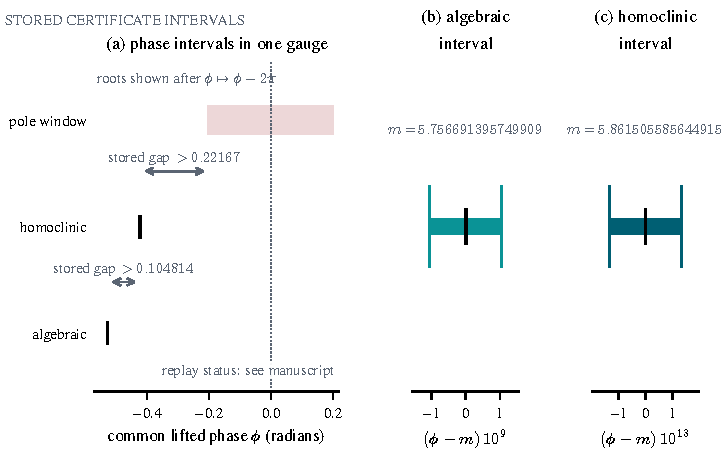
\includegraphics[width=\textwidth]{figures/validated_source_phase_separation.pdf}
\caption{Validated separation of the source phases on the circle
$\|u\|=0.01$ in the common linearizing phase coordinate.
\textup{(a)} The interval-enclosed algebraic and symmetric-homoclinic
roots are shown after subtracting $2\pi$, together with the closed
pole-entry cover $[-0.2,0.2]$.  The arrows give rigorous lower bounds for
the consecutive gaps.  \textup{(b,c)} The complete algebraic and
homoclinic root enclosures are magnified about their interval midpoints
$m$.  Thick segments are the full interval enclosures; black ticks are
arithmetic midpoints used only for plotting and are not additional
numerical evidence.}
\label{fig:validated-source-phases}
\end{figure}

Here is the finite cell and incidence check used by the abstract theorem.
Choose mutually disjoint compact subapertures inside those phase gaps and
take their boundaries, together with transverse flowbox exit faces, as the
functions $h_j$ in \eqref{eq:face-sign-strata}.  Name every connected
stratum in the complement of the three outgoing subapertures as an
outgoing-box lateral outcome.  At the end of the homoclinic tube, name
every complementary stratum outside the re-entry aperture and the stable
cut as a return-box lateral outcome.  Their closures, together with the
three apertures, re-entry strata, and cut, cover the two chosen compact
bands, so the return/first-exit assignment is total.  On every nonempty active
set their conormals are independent by the flowbox construction.  The
finite identities \eqref{eq:finite-cell-cover} on $B^u$ and $B^r$ then give
all two-dimensional interiors, one-dimensional faces, and zero-dimensional
corners.  Choose the artificial faces of the signed reference cell in the
certified phase gaps and transverse to the finitely many pulled-back active
strata; a generic compact interior choice has this property.  The certified
homoclinic and algebraic phase-derivative bounds, the open pole window, and
the flowbox faces then give the pullback rank and boundary-neatness margins
required in \textup{(H2)}.  The interval event bounds above, homoclinic transversality, and
the algebraic graph margins remain strict on slightly smaller compact
subapertures; the artificial lateral faces are transverse to the flow by
construction.  Compactness gives one positive minimum for event speed,
competing-face sign, and event-order distance.  The certified algebraic
root and a point in the interior pole-entry interval lie a positive
distance from the boundary of the chosen signed reference cell.  Under the
cut-face templates \eqref{eq:limiting-signed-exit-template} they give the
two interior anchors required in \textup{(H2)}.  This verifies the
exhaustive list of labelled connected strata, nonemptiness of both end channels,
and all first-exit margins without
inferring a global partition outside the fixed flow-tube domain.

For the Markov-strip hypothesis take the two vertices $\Sigma_+$ and
$\Sigma_-$.  For every $(\sigma,n)$,
Proposition~\ref{prop:selector} gives one closed strip
$\widetilde{\mathcal V}_{\sigma,n}$ in its fixed matching tube before the target cut.  The target
set $\bar\nu=0$ cuts it exactly as in
\eqref{eq:parent-strip-cut}: the two nonempty regular components are the
edges $a=(\sigma,n,\sigma')$, while
$\mathcal I_{\sigma,n}=E_{\mathrm{cut},\sigma,n,1}$ is a first-exit face.  The two
vertex charts \eqref{eq:signed-vertex-charts} give every edge a completed
cross form on $I\times J$.  In particular,
\eqref{eq:half-edge-cross-forms} uses the same positive magnitude coordinate
at the source and target vertices, while
\eqref{eq:branch-seam-scale}--\eqref{eq:scaled-seam-bounds} supply its
field-dependent rescaled transverse-action margin.
The first-hit Poincar\'e map sends that edge diffeomorphically to a
horizontal strip in $\Sigma_{\sigma'}$, and the flowbox rectangles give one full
horizontal--vertical crossing exactly when the preceding target sign is
the following source sign.  Unequal vertices are not composable.

The signed normal in \eqref{eq:signed-normal-scale}, the strict phase
monotonicity \eqref{eq:local-phase-monotonicity}, and the half-open angular
lift make the triples $(\sigma,n,\sigma')$ faithful and the regular domains
disjoint.  They also prove local finiteness away from the two source cut
faces and identify the two fixed-source-sign high-winding families, while
retaining the target sign.  Thus the return graph satisfies the
Markov-strip hypothesis, and \eqref{eq:local-relative-partition} places
the zero-action boundary in exactly one first-exit component.

The rigorous numerical enclosures for the three source orbits and the
independent finite collar are documented in
Section~\ref{app:computer-proof}.  Together with the analytic arguments of
Sections~\ref{sec:passage} and \ref{sec:terminal}, the first-table margins
verify the common hypotheses of Theorems~\ref{thm:main}--
\ref{thm:coding-persistence}.  That appendix also states
the mathematical validation criteria and reproduction procedure.
No low-winding or larger-section statement is imported into this
verification.

\subsection{Optional module: the selected reversible branch from the algebraic connection}
\label{sec:optional-selected-branch}

\begin{proposition}[Continuation to the first nondegenerate critical point]
\label{prop:exact-source-outer-fold}
Let $\mathcal W_{\rm a}$ be the canonical finite saturation
\eqref{eq:algebraic-finite-saturation}.  There is a connected
$C^2$ arc
\begin{equation}\label{eq:exact-source-arc}
 c(U)=(U,0,V(U),0)\in\mathcal W_{\rm a}\cap\Fix\cR,
 \qquad 0\le U\le U_f,
\end{equation}
with
\begin{equation}\label{eq:c0}
 \begin{gathered}
 c(0)=c_0=(0,0,1/6,0),\\
 U_f\in[.041527012176079285,.041527012805834346].
 \end{gathered}
\end{equation}
The restriction $E(c(U))$ has no critical point for $0\le U<U_f$ and has
one nondegenerate critical point at $U_f$.  Thus this is the first critical
point of the restricted Hamiltonian on the selected arc followed from
$c_0$.
\end{proposition}

\begin{proof}
The proof has one analytic and one validated finite part.  Appendix~\ref{app:jost-source-arm} constructs an exact Jost basis along the algebraic orbit, proves that the canonical tangent is
\[
 \operatorname{span}\{(1,0,-2k_0,0)\},
 \qquad
 k_0=\frac{\sqrt\pi\,\Gamma(1/4)}
 {4\sqrt6\,\Gamma(3/4)},
\]
and excludes the growing Jost mode from the weighted tangent bundle.  A
fixed-$U$ interval continuation starting from this analytic tangent then
keeps $dE(c(U))/dU<0$ up to the final cap, where an augmented Krawczyk
argument proves one simple zero and identifies it with the first
nondegenerate critical point on the connected selected arc.  The exact
representations, exclusion
argument, continuation bridges, and numerical margins are recorded in
that appendix.
\end{proof}

A fixed critical-point/event continuation follows the other local side of
this critical point into
a $6{,}316$-box intermediate collar.  A further $9{,}725$-box continuation,
joined by $9{,}724$ true common-root containments, reaches the circle
$r=2.4\times10^{-4}$.  Fixed-radial uniqueness identifies its endpoint with
the local branch in \eqref{eq:source-spiral}.  The full-state identification
shared by the validated continuations therefore joins these pieces into one
selected connected branch from $c_0$ through the first critical point to the local
logarithmic spiral.  No assertion is made about other components of
$\mathcal W_{\rm a}\cap\Fix\cR$.

\subsection{Intrinsic realization and the normal-form corollary}

\begin{proposition}[Intrinsic realization by the normal-form system]
\label{prop:core-intrinsic-realization}
For the one-point parameter space, the system
\eqref{eq:core-intro}, with the fixed local return--exit tube constructed
in this section, is an intrinsic two-ended Hamiltonian configuration in
the sense of Definition~\ref{def:intrinsic-two-end-data}.
\end{proposition}

\begin{proof}
We match the five clauses of the definition.  For \textup{(I1)},
\eqref{eq:core-primitive}--\eqref{eq:core-reverser} are polynomial and
satisfy $\mathcal R^*\lambda=-\lambda$; the origin has
$\alpha_0=\beta_0=2^{-1/2}$.  The fixed local saddle block may be chosen
inside the analytic normal-form ball, with auxiliary radial faces joined
to its physical faces by compact event-free orbit slides.

For \textup{(I2)}, the determinant enclosure
\eqref{eq:hom-det} and the independent tangent rows
\eqref{eq:hom-tangent-U}--\eqref{eq:hom-tangent-V} prove transversality of
the selected homoclinic in the regular critical-energy hypersurface.  For
\textup{(I3)}, the finite flowbox construction in
lines~\eqref{eq:hom-phase}--\eqref{eq:hom-det} and the incidence check
following Figure~\ref{fig:validated-source-phases} give the clean physical
event stratification, neat boundary faces, strict first-hit order, and the
two interior anchors.  The certified phase gaps allow the physical source
cell and its two signed limiting traces to be placed in one proper arc
with a complementary cut interval of positive length.

For \textup{(I4)}, Proposition~\ref{prop:core-algebraic-future} provides
the algebraic compactification, the product interval block, and the
physical finite saturation.  The energy-face and flag ranks follow from
the validated coordinate system and
\eqref{eq:validated-energy-faces}.  The block bounds
\eqref{eq:validated-algebraic-block-bounds} and the positive gaps
\eqref{eq:validated-algebraic-cone-rates}--
\eqref{eq:validated-four-rate-gaps}, inserted into
\eqref{eq:block-to-finite-time-bunching}, give the intrinsic finite-time
secant-cone and order-three bunching inequalities (indeed also the optional
fourth gap).  Finally,
\eqref{eq:pole-coordinates}--\eqref{eq:core-pole-indicial-matrix} give the
analytic pole chart, boundary sink, and simple indicial spectrum
$\{1,4,6\}$ with $m_{\mathrm p}=6$; together with
\eqref{eq:core-action-density} they also show directly that
$\rho^6\lambda(X)$ extends in $C^9=C^{m_{\mathrm p}+3}$.
Propositions~\ref{prop:pole-cone}
and \ref{prop:pole-cone-to-sink}, with
\eqref{eq:pole-validated-time}--\eqref{eq:pole-validated-speeds}, supply
the compact basin entry and strict radial margins required in
\textup{(I5)}.  Thus all
intrinsic clauses hold for the same fixed physical tube.
\end{proof}

\begin{corollary}[Relative openness near the normal-form system]
\label{cor:core-relative-open-class}
Fix an integer $k\ge5$, the physical saddle block, finite flow tubes, cooriented event
hypersurface germs, and the two compactifications used above.  Fix also
$m_{\mathrm p}=6$ and the indicial conjugacy class
\eqref{eq:core-pole-indicial-matrix}.  In the space of reversible exact
Hamiltonians that are analytic on the saddle germ, $C^k$ on the compact
and algebraic tubes, and $C^9$ on the pole compactification, restrict to
the subspace preserving the algebraic boundary factorizations, every
designated structurally invariant face, and this pole indicial conjugacy
class.  There is a relatively open neighborhood $\mathcal O$ of the
normal-form system such that every Hamiltonian in $\mathcal O$ satisfies
the hypotheses of Theorem~\ref{thm:main-result} on the continued physical
tube.  On each compact $K\subset\mathcal O$, the state-only strict margins
and the threshold for time spent in the saddle block can be chosen
uniformly.  If a compact finite-dimensional $C^r$ family, $r\le2$, has
image in $K$, then after fixing
\[
 0<\kappa<\inf_{H\in K}\frac{2\pi\alpha_H}{\beta_H},
\]
the mixed state--parameter conclusions of
Theorem~\ref{thm:main-result} hold; constants involving parameter
derivatives may depend on the $C^r$ norm of that family.
\end{corollary}

\begin{proof}
The symmetric homoclinic persists by its transverse intersection, and the
finite clean first-hit stratification, its exhaustive labelled strata, the
proper-arc condition, and both end anchors persist because all defining
rank, first-hit, event-order, and boundary margins are strict on compact
sets.  Proposition~\ref{prop:algebraic-normal-persistence} continues the
locally maximal normally expanding algebraic hypersurface and preserves
the order-three bunching inequalities.  The hyperbolic pole sink, its
common basin-entry neighborhood, and the radial and spectral-gap margins
persist inside the fixed indicial class.  The local chart-production
theorem then supplies the marked representations; no eigenframe or angular
lift is included in the perturbation data.  Compactness gives the uniform
state-only margins and threshold on $K$.  The parameter statement then
follows from Theorem~\ref{thm:coding-persistence}\textup{(ii)} with the
stated strict rate gap and its explicit dependence on the family norm.
\end{proof}

\begin{remark}[Why the openness is relative]
Corollary~\ref{cor:core-relative-open-class} is not an assertion in an
unrestricted compact-open $C^k$ topology.  Such a topology neither
preserves state analyticity at the saddle nor controls extensions to the
two chosen compactifications, and it allows the pole indicial roots to
move through resonances.  Removing those restrictions would require a
finite-smooth saddle passage with the present weighted parameter bounds
and a polyhomogeneous pole calculus with moving exponents.  Neither is
proved here.
\end{remark}

\begin{proof}[Proof of Corollary~\ref{cor:core}]
Proposition~\ref{prop:core-intrinsic-realization} shows that the core is an
intrinsic two-ended Hamiltonian configuration, so
Theorem~\ref{thm:main-result} applies, after the fixed compact
source-subcell restriction, on the region defined by sufficiently long
physical saddle-block residence time within that subcell.
In the locally produced marking, the exact calculations and interval
enclosures in this section verify \textup{(H1)}--\textup{(H4)} of
Definition~\ref{def:two-ended-hypotheses}.
For every fixed $\kappa\in(0,2\pi)$, the critical-energy flow of
\eqref{eq:core-intro} has the high-winding return--exit decomposition, exact
renormalized roof/action cocycle, two-sided countable coding, stable
plaques, and the compactification by the two limit points $0^\pm$ from
Theorems~\ref{thm:main}--
\ref{thm:coding-persistence}.  Corollary~\ref{cor:period-action-asymptotics}
and Theorem~\ref{thm:tail-entropy-action} give the remaining conclusions
stated in Corollary~\ref{cor:core}.
\end{proof}

\subsection{Optional selected-branch consequence for the normal-form system}

\begin{corollary}[Optional selected branch for the normal-form system]
\label{cor:core-selected-branch}
The algebraic connection in
Proposition~\ref{prop:core-origin-algebraic} selects a reversible branch
whose successive critical points have physical Euclidean $(U,V)$ radii
satisfying
\begin{equation}\label{eq:core-fold-ratio}
 \frac{R_{UV,m+1}}{R_{UV,m}}
 =e^{-\pi/2}\bigl(1+O(R_{UV,m}^{\widehat\eta})\bigr),
 \qquad \widehat\eta=\min\{\eta,1\}.
\end{equation}
The validated finite continuation extends this selected branch from the
local annulus through its first nondegenerate critical point to the exact
algebraic source $c_0$.
\end{corollary}

\begin{proof}
Proposition~\ref{prop:core-origin-algebraic} verifies the additional
transverse algebraic connection required in
Corollary~\ref{cor:source-fold-persistence}.  Choose the marked cross-form
chart tangent to the linear
coordinates \eqref{eq:core-linear-saddle-coordinates}.  On $\Fix\cR$ its
unstable coordinate obeys $u=\xi+O(|\xi|^2)$ through the required logarithmic
jets, while $(U,V)=2(u_1,u_2)$ in the linear chart.  Consequently the
physical radius satisfies $R_{UV}=2r(1+O(r))$; inserting
$\alpha_0=\beta_0$ into \eqref{eq:fold-ratio} gives
\eqref{eq:core-fold-ratio}.  Proposition~\ref{prop:exact-source-outer-fold}
and the subsequent continuation establish the final assertion.
\end{proof}

\section{Optional perspective: orbit-preserving genericity of transverse matching}
\label{sec:matching-genericity}

The nonzero derivative used in the finite homoclinic matching is not
forced by the saddle-focus or by either compactified end.  The following
proposition shows that its failure is locally of codimension one under
reversible Hamiltonian perturbations supported in the compact part of the
orbit.  The perturbations keep the selected connection itself fixed.  This
is an auxiliary transversality result; it is not used by the main theorem
and does not provide a second system-level application.

\begin{proposition}[Orbit-preserving genericity of transverse matching]
\label{prop:matching-transversality}
Let $k\ge5$, let $\mathbf X\in\mathfrak H_{\mathrm{adm}}^k$, and suppose
the chosen compact Hamiltonian flow-box coordinates are $C^{k+2}$.
Let $\Gamma$ be a regular symmetric critical-energy homoclinic orbit in
the fixed compact flight tube.  Write
$p=\Gamma\cap\Fix\mathcal R$ and let $\psi_*$ be its source phase in
\eqref{eq:finite-homoclinic-map}.  Choose an open Hamiltonian flow box
$U$ on the unstable half of $\Gamma$, away from the saddle chart, all
marked sections, all event faces, and both end charts, so small that
\[
 \overline U\cap\mathcal R(\overline U)=\varnothing,
\]
and such that $(\overline U\cup\mathcal R(\overline U))\cap\Gamma$
consists only of the chosen orbit segment and its reflected symmetric
segment.  Fix $U_0\Subset U$.

Let $\mathcal K_\Gamma^{k+2}(U_0)$ be the closed Banach subspace of
$C^{k+2}$ functions $K$ supported in
$\overline U_0\cup\mathcal R(\overline U_0)$ such that
\begin{equation}\label{eq:orbit-preserving-hamiltonian-space}
 K\circ\mathcal R=K,\qquad K|_\Gamma=0,\qquad dK|_\Gamma=0.
\end{equation}
For $K$ sufficiently small set
\[
 H^K=H+K,\qquad \iota_{X^K}\omega=dH^K,
\]
and retain the original primitive, reverser, sections, and marked charts.
Then $\mathbf X^K\in\mathfrak H_{\mathrm{adm}}^k$, the parametrized orbit
$\Gamma$ is unchanged, and the compact transition has the form
\[
 (\bar\phi,\bar\nu)
   =\bigl(f_K(\psi,\nu_u),g_K(\psi,\nu_u)\bigr)
\]
near $(\psi_*,0)$.  The matching determinant
\begin{equation}\label{eq:matching-determinant-evaluation}
 \mathfrak d(K):=\partial_\psi g_K(\psi_*,0)
\end{equation}
is a $C^1$ function of $K$.  At every sufficiently small $K_0$ for which
$\mathfrak d(K_0)=0$, its derivative
\[
 D\mathfrak d(K_0):
 \mathcal K_\Gamma^{k+2}(U_0)\longrightarrow\mathbb R
\]
is onto.  Consequently, near each such $K_0$, the set
$\mathfrak d^{-1}(0)$ is a $C^1$ codimension-one Banach submanifold.
Equivalently, there is a $C^{k+2}$ reversible Hamiltonian $K_*$ in this
space for which
\begin{equation}\label{eq:matching-determinant-crossing}
 \left.\frac d{d\varepsilon}\right|_{\varepsilon=0}
 \mathfrak d(K_0+\varepsilon K_*)\ne0.
\end{equation}

The same conclusion holds for the origin-to-algebraic connection if
\eqref{eq:matching-determinant-evaluation} is replaced by
\begin{equation}\label{eq:algebraic-determinant-evaluation}
 \mathfrak d_{\mathrm a}(K)
 =Dg_{\mathrm a}(q_*)\,DP_{\mathrm a}^{K}(z_*)v_*.
\end{equation}
Here $P_{\mathrm a}^{K}$ is the compact first-hit map from the fixed
unstable source trace to a section on which the algebraic future trace has
defining function $g_{\mathrm a}$, and $v_*$ is the nonzero source-phase
tangent.  Assume that $Dg_{\mathrm a}(q_*)$ restricts to a nonzero covector
on the critical-energy target section, equivalently that its pullback by
the finite flight is nonzero on the critical-energy symplectic normal
plane.  In this case define
$\mathcal K_\Gamma^{k+2}(U_0)$ with $\Gamma$ equal to the selected
origin-to-algebraic orbit and choose
$U\cup\mathcal R(U)$ also disjoint from the fixed future tail defining
$g_{\mathrm a}$, with
$\mathcal R(\overline U)\cap\Gamma=\varnothing$ and
$\overline U\cap\mathcal R(\Gamma)=\varnothing$.  Formula
\eqref{eq:algebraic-determinant-evaluation} is the section form of
\eqref{eq:algebraic-terminal-transversality-row}.

In either case, within the orbit-preserving perturbation space the
nondegenerate subset is locally open and dense.  All other strict
return--exit hypotheses persist on their relatively open subset, while
the saddle passage, clock, primitive, algebraic coefficients, and pole
boundary jet are unchanged.
\end{proposition}

\begin{proof}
An $\mathcal R$-invariant Hamiltonian has a reversible Hamiltonian vector
field because $\mathcal R$ is anti-symplectic.  Moreover $K=dK=0$ on
$\Gamma$, and hence $X^K=X$ there.  Thus the orbit, including its time
parametrization, is fixed.  The support condition leaves the local
saddle-focus passage and clock, the algebraic factorization, and the pole
boundary jet unchanged.  It also leaves the primitive fixed.  Therefore a
small $K$ gives a presentation in $\mathfrak H_{\mathrm{adm}}^k$; the
strict compact first-hit inequalities persist after decreasing its norm.
Standard finite-time dependence of an ODE on its $C^k$ vector field shows
that \eqref{eq:matching-determinant-evaluation} is $C^1$ in the
$C^{k+2}$ Hamiltonian.

We first treat the symmetric homoclinic.  Replacing $H$ by $H^{K_0}$, if
necessary, reduces the submersion assertion at an arbitrary zero $K_0$ to
the case $K_0=0$; the orbit and every support condition are unchanged.
Since $p$ is a regular point of $H^{-1}(0)$, the quotient
\[
 N_p=\ker dH(p)/\operatorname{span}\{X(p)\}
\]
is a symplectic plane, with reduced form $\omega_p^{\mathrm{red}}$.
The reverser induces an anti-symplectic involution $R_p$ on $N_p$.  If
$v_K\ne0$ spans the image of $T_pW^u(O)$ in $N_p$, then $R_pv_K$ spans
the corresponding stable line.  Hence
\begin{equation}\label{eq:reduced-homoclinic-determinant}
 \delta(K)=\omega_p^{\mathrm{red}}(v_K,R_pv_K)
\end{equation}
vanishes exactly when the stable and unstable manifolds fail to be
transverse modulo their common flow direction.  Passing between the
reduced plane and the fixed source and target section coordinates
multiplies \eqref{eq:reduced-homoclinic-determinant} by a nonzero $C^1$
factor.  Thus
\begin{equation}\label{eq:matching-reduced-factor}
 \mathfrak d(K)=a(K)\delta(K),\qquad a(K)\ne0.
\end{equation}

It remains to vary $\delta$ while fixing $\Gamma$.  By the Hamiltonian
flow-box theorem, after shrinking $U$ there are $C^{k+2}$ coordinates
$(t,E,x,y)$ in which
\[
 \omega=dt\wedge dE+dx\wedge dy,\qquad
 H=E,\qquad
 \Gamma\cap U=\{E=x=y=0\}.
\]
The transverse coordinates may be chosen so that the transported unstable
direction at the entrance to $U$ is $\partial_x$.  Choose
$\chi\in C_c^\infty(\mathbb R)$ supported in the $t$-interval of $U_0$
with $\int\chi(t)\,dt=1$.  With a transverse cutoff equal to one near
$E=x=y=0$, put
\[
 \varkappa(t,E,x,y)=\frac12\chi(t)x^2
\]
in $U$ and extend it by zero.  Its reversible extension is
\begin{equation}\label{eq:reversible-quadratic-shear}
 K_*=\varkappa+\varkappa\circ\mathcal R.
\end{equation}
It belongs to $\mathcal K_\Gamma^{k+2}(U_0)$.  On the unstable half of
$\Gamma$ the second summand is absent, and the transverse variational
equation for $H+\varepsilon K_*$ is
\[
 \dot x=0,\qquad \dot y=-\varepsilon\chi(t)x.
\]
Thus passage through $U$ changes the unstable direction by the
symplectic shear
\begin{equation}\label{eq:normal-shear}
 (x,y)\longmapsto(x,y-\varepsilon x).
\end{equation}
After the fixed transport from $U$ to $p$, this realizes
$v_\varepsilon=v_0+\varepsilon w+O(\varepsilon^2)$ with
$\omega_p^{\mathrm{red}}(v_0,w)\ne0$.  The reflected bump lies on the
stable half and ensures reversibility; the stable direction at $p$ is
$R_pv_\varepsilon$.

Suppose now that $\delta(0)=0$.  In a symplectic plane the lines spanned
by $v_0$ and $R_pv_0$ then coincide.  Differentiating
\eqref{eq:reduced-homoclinic-determinant} and using the anti-symplectic
identity gives
\begin{align*}
 \delta'(0)
 &=\omega_p^{\mathrm{red}}(w,R_pv_0)
   +\omega_p^{\mathrm{red}}(v_0,R_pw)\\
 &=2\omega_p^{\mathrm{red}}(w,R_pv_0)\ne0.
\end{align*}
Together with \eqref{eq:matching-reduced-factor}, this proves
\eqref{eq:matching-determinant-crossing}.  The Banach-space implicit
function theorem gives the codimension-one assertion.

For the algebraic connection, pull the target conormal
$Dg_{\mathrm a}(q_*)$ back to the symplectic normal plane at the exit of
$U$.  At a zero of
\eqref{eq:algebraic-determinant-evaluation} it annihilates the transported
source tangent but is not the zero covector by the explicit target-section
assumption.  Choose the transverse
coordinates so that the shear \eqref{eq:normal-shear} moves that tangent
in a direction on which the pulled-back conormal is nonzero.  The same
calculation then gives $\mathfrak d_{\mathrm a}'(0)\ne0$.  Because
$U\cup\mathcal R(U)$ is disjoint from the fixed algebraic tail, its
defining function and all end coefficients are unchanged.  This proves
the last assertion.  The local openness and density follow from the
submersion result and the openness of the remaining strict margins.
\end{proof}

\begin{remark}[Scope of Proposition~\ref{prop:matching-transversality}]
The proposition concerns loss of transversality of a selected
critical-energy connection.  It neither asserts that such a connection
exists for a generic Hamiltonian nor describes the boundary of the set on
which all return, first-exit, and end hypotheses hold uniformly over a
compact corridor.  Its content is that, once the selected
connection is present, exactness, reversibility, the fixed saddle passage,
and the two end compactifications do not force its matching determinant to
vanish: a one-parameter orbit-preserving reversible Hamiltonian family crosses the
degeneracy set while preserving the orbit itself.  This is a local
genericity theorem for each selected connection separately; it does not
provide a second system-level application.
\end{remark}

\section{Scope and remaining questions}
\label{sec:scope}

The theorem has four precise scope limits.  First, it concerns a fixed
local flow tube and a compact source subcell: low windings are excluded,
and no assertion is made about an orbit after it crosses a lateral face or
about a global critical-energy partition.  Second, the local coordinates
are produced in the state-analytic saddle and geometric two-end class of
Definition~\ref{def:intrinsic-two-end-data}, not for an arbitrary
unmarked $C^k$ Hamiltonian family.  Third, persistence is taken in the
relative coefficient topology that fixes the physical block and tubes,
the cooriented event germs, and the indicated end structures; unrestricted
ambient openness is not claimed.  Fourth, the pole theorem fixes the
compactified-action order and the simple positive-integer indicial
conjugacy class.  The finite boundary jet may vary, but the indicial roots
do not move or cross a resonance.

Two natural extensions are therefore clear.  A larger dynamical result
would validate the finitely many low windings and every new first-exit face
in a larger flow tube.  A broader pole theorem would allow moving indicial
roots and resonance crossings; this requires parameter-dependent powers
and uniform divided-difference coordinates rather than the fixed finite
recursion used here.

Within these limits, an intrinsic saddle-focus configuration with a
transverse homoclinic tube, clean physical event geometry, and the two end
compactifications produces finitely many parameter-local reversible exact
symplectic coordinate systems.  Above one common residence-time cutoff,
they determine the same exhaustive physical return/first-exit relation.
The classical countable bifocal return dynamics then carries strict
first-exit events, two compatible action finite parts, exact action
composition, and mixed state--parameter control.

\appendix

\section{A computable criterion for the algebraic end}
\label{app:algebraic-interval-criterion}

This appendix records the interval-block criterion used to verify the
normally expanding algebraic hypersurface in the normal-form application.
It is a sufficient test for the geometric hypothesis in
Definition~\ref{def:intrinsic-two-end-data}; its product coordinates and
cone constants are not inputs to the return--exit theorem.

\begin{theorem}[Interval-block criterion for a normally expanding
hypersurface]
\label{thm:algebraic-corridor-graph}
Let $\mathcal P$ be a compact finite-dimensional parameter manifold, let
$r\in\{0,1,2\}$, and let
\begin{equation}\label{eq:corridor-field-family}
 \varpi\longmapsto Y_\varpi=(F_\varpi,G_\varpi)
\end{equation}
be a $C^r$ map into the $C^5$ vector fields on a fixed collar of an
oriented $C^5$ interval bundle $\pi:Q_\Gamma\to B_\Gamma$, where
$B_\Gamma$ is a compact manifold with corners.  Fix an oriented $C^5$
trivialization $Q_\Gamma\simeq
B_\Gamma\times[-\zeta_\Gamma,\zeta_\Gamma]$, its product splitting, and
adapted base and fiber metrics.  Suppose every base face is
strictly inward or is structurally invariant throughout the chosen
coefficient class, and the two fiber faces are strict exits.

Assume that $Q_\Gamma$ has a fixed ambient interval collar
\[
 \widehat Q_\Gamma=
 B_\Gamma\times[-\zeta_\Gamma-\varepsilon_\Gamma,
                 \zeta_\Gamma+\varepsilon_\Gamma]
 \supset Q_\Gamma
\]
on which the bundle projection, product splitting, adapted metrics, and
the time-$\delta_{\mathrm g}$ map extend for some
$\delta_{\mathrm g}>0$.  The normal component retains its strict outward
sign beyond the two fiber faces.  Fix a closed vertical cone and a closed
horizontal Grassmann cone $\mathcal H_{\varpi,z}$ of base-dimensional
graphs of slope at most $\alpha_{\mathrm g}$.  We require the following
two conditions.

First, the vertical cone is strictly forward invariant with a uniform
angular margin.  Whenever two orbit segments stay in the ambient collar,
a separation initially in this cone remains in its interior and its
vertical component grows at least as $e^{\lambda_{\mathrm g}s}$ for one
$\lambda_{\mathrm g}>0$.  In addition, if
$z'=\Phi_\varpi^{\delta_{\mathrm g}}z$ and
$P_+\in\mathcal H_{\varpi,z'}$, then all backward planes
\[
 (D\Phi_\varpi^{\delta_{\mathrm g}-s})^{-1}P_+,
 \qquad 0\le s\le\delta_{\mathrm g},
\]
belong to the corresponding horizontal cones, and the initial plane lies
in their relative interior.  We refer to these requirements as the
uniform secant-cone and backward projectivized-cone conditions.

Second, call a base-dimensional plane
$P\subset T_z\widehat Q_\Gamma$, $z\in Q_\Gamma$,
$\delta_{\mathrm g}$-admissible if the orbit segment stays in the ambient
collar and every plane $P_s=D\Phi_\varpi^sP$ belongs to
$\mathcal H_{\varpi,\Phi_\varpi^sz}$ for
$0\le s\le\delta_{\mathrm g}$.  Put
$P'=P_{\delta_{\mathrm g}}$ and $z'=\Phi_\varpi^{\delta_{\mathrm g}}z$,
and define
\begin{align*}
 A^\delta_{\varpi,z}(P)
  &=d\pi_{z'}\circ D\Phi_\varpi^{\delta_{\mathrm g}}|_P
       \circ(d\pi_z|_P)^{-1},\\
 N^\delta_{\varpi,z}(P)
  &:T_z\widehat Q_\Gamma/P
       \longrightarrow T_{z'}\widehat Q_\Gamma/P'.
\end{align*}
Use the base metric for $A^\delta$.  If
$V_z=\ker d\pi_z$ and
$q_P:T_z\widehat Q_\Gamma\to T_z\widehat Q_\Gamma/P$ is the quotient
map, transport the fiber metric to the quotient through
$q_P|_{V_z}$, and use the analogous norm at $P'$.  Thus, for
$P=\operatorname{graph}S$, the quotient coordinate is
$[(u,v)]\mapsto v-Su$.  Assume the finite-time order-three inequalities
\begin{equation}\label{eq:alg-intrinsic-rate-gaps}
 \vartheta_{\mathrm g,j}:=
 \sup_{\substack{\varpi\in\mathcal P,\ z\in Q_\Gamma\\
                  P\ \delta_{\mathrm g}\text{-admissible}}}
 \bigl\|(N^\delta_{\varpi,z}(P))^{-1}\bigr\|
 \bigl\|A^\delta_{\varpi,z}(P)\bigr\|^j<1,
 \qquad j=0,1,2,3.
\end{equation}

These hypotheses can be verified in one global adapted product chart by
coefficient bounds.  Write
\[
 DY_\varpi=
 \begin{pmatrix}C_\varpi&B_\varpi\\D_\varpi&a_\varpi\end{pmatrix}
\]
in base--fiber blocks.  It is sufficient that, on a fixed neighborhood of
$Q_\Gamma$, for some positive constants independent of $\varpi$,
\begin{equation}\label{eq:alg-normal-exit-faces}
 G_\varpi(x,-\zeta_\Gamma)\le-m_{\mathrm g}<0
 <m_{\mathrm g}\le G_\varpi(x,\zeta_\Gamma),
 \qquad x\in B_\Gamma,
\end{equation}
and
\begin{equation}\label{eq:alg-block-bounds}
 \mu_2(C_\varpi)\le c_{\mathrm g},\qquad
 \|B_\varpi\|\le b_{\mathrm g},\qquad
 \|D_\varpi\|\le d_{\mathrm g},\qquad
 a_\varpi\ge a_{\mathrm g}.
\end{equation}
Require the vertical-cone and normal-growth margins
\begin{equation}\label{eq:alg-cone-growth-margins}
 q_{\mathrm g}:=\alpha_{\mathrm g}(a_{\mathrm g}-c_{\mathrm g})
       -d_{\mathrm g}-b_{\mathrm g}\alpha_{\mathrm g}^2>0,
 \qquad
 \lambda_{\mathrm g}:=a_{\mathrm g}
       -d_{\mathrm g}/\alpha_{\mathrm g}>0,
\end{equation}
and the order-three rate gaps
\begin{equation}\label{eq:alg-jet-rate-gaps}
 \gamma^{\rm chart}_{\mathrm g,j}:=a_{\mathrm g}-j c_{\mathrm g}
       -(j+1)b_{\mathrm g}\alpha_{\mathrm g}>0,
 \qquad j=0,1,2,3.
\end{equation}
Then the cone conditions above hold and, along every admissible segment,
\begin{equation}\label{eq:block-to-finite-time-bunching}
 \begin{aligned}
 \|A^\delta_{\varpi,z}(P)\|
 &\le e^{(c_{\mathrm g}+b_{\mathrm g}\alpha_{\mathrm g})\delta_{\mathrm g}},\\
 m(N^\delta_{\varpi,z}(P))
 &\ge e^{(a_{\mathrm g}-b_{\mathrm g}\alpha_{\mathrm g})\delta_{\mathrm g}},\\
 \vartheta_{\mathrm g,j}
 &\le e^{-\gamma^{\rm chart}_{\mathrm g,j}\delta_{\mathrm g}}<1.
 \end{aligned}
\end{equation}
One may instead verify the coordinate-independent finite-time conditions
directly; bounds obtained by taking unrelated extrema in different charts
are not used.

Under these hypotheses, the
maximal forward-staying set
\begin{equation}\label{eq:maximal-forward-staying-set}
 \mathcal W^{\rm tail}_\varpi
 =\{z\in Q_\Gamma:\Phi^s_\varpi z\in Q_\Gamma
       \text{ for every }s\ge0\}
\end{equation}
is the image of a unique section $\Gamma_\varpi:B_\Gamma\to Q_\Gamma$.
In the chosen adapted trivialization it is the graph
\begin{equation}\label{eq:parameterized-algebraic-graph}
 \zeta=\Gamma_\varpi(x),\qquad x\in B_\Gamma,\qquad
 \|D_x\Gamma_\varpi\|\le\alpha_{\mathrm g}.
\end{equation}
It is normally expanding (hence locally repelling) in forward
desingularized time.  Equivalently,
the local backward graph transforms contract its normal jets.
For $P=T_z\mathcal W^{\rm tail}_\varpi$, the tangent and normal quotient
maps in the criterion coincide, under the base identification, with
those in \eqref{eq:intrinsic-algebraic-normal-bunching}; hence
$\vartheta_{\mathrm a,j}\le\vartheta_{\mathrm g,j}<1$ for
$0\le j\le3$.

The graph has the scale regularity
\begin{equation}\label{eq:algebraic-graph-scale-regularity}
 \sup_{\substack{i+j\le3\\j\le r}}
 \sup_{(x,\varpi)\in B_\Gamma\times\mathcal P}
 \bigl|D_x^iD_\varpi^j\Gamma_\varpi(x)\bigr|<\infty.
\end{equation}
Thus, in parameter charts,
\begin{equation}\label{eq:algebraic-graph-scale-spaces}
 \Gamma\in C^0(\mathcal P;C^3(B_\Gamma))
 \cap C^1(\mathcal P;C^2(B_\Gamma))
 \cap C^2(\mathcal P;C^1(B_\Gamma)),
\end{equation}
with the last one or two factors omitted when $r<2$.  If the additional
intrinsic finite-time gap
\begin{equation}\label{eq:alg-fourth-rate-gap}
 \vartheta_{\mathrm g,4}:=
 \sup_{\varpi,z,P\ {\rm admissible}}
                 \bigl\|(N^\delta_{\varpi,z}(P))^{-1}\bigr\|
                 \bigl\|A^\delta_{\varpi,z}(P)\bigr\|^4<1
\end{equation}
holds, then every state graph is $C^4$, with a uniform $C^4$ bound.  All
these conclusions persist on a sufficiently small $C^5$ coefficient
neighborhood relative to the subspace preserving every designated
structurally invariant base face.  If all base faces are strictly inward,
this is an ordinary $C^5$ neighborhood.  Constants involving parameter
derivatives may depend on the $C^r$ norm of the chosen family.
\end{theorem}

\begin{proof}
An oriented interval bundle is trivial because the orientation-preserving
diffeomorphism group of an interval is contractible; the theorem fixes one
such trivialization before stating the cone and bunching bounds.  All
differential estimates below use its adapted metrics and a finite corner
atlas on the base.  We separate
existence and uniqueness from differentiability.  Fix
$\varpi$ and $x\in B_\Gamma$.  Among the initial values
$\zeta\in[-\zeta_\Gamma,\zeta_\Gamma]$, let $L_x$ and $U_x$ consist of
those whose first exit is through the lower and upper normal face,
respectively.  No orbit can leave through a base face.  The strict normal
face inequalities make $L_x$ and $U_x$ disjoint relatively open sets, and
they contain the two endpoints.  If no initial value stayed for all
positive time, these two sets would disconnect the interval.  Hence every
fiber contains a forward-staying point.

For two orbit segments contained in one product/base chart write their separation
as $(u,v)$ in base and normal coordinates.  Under the one-chart sufficient
criterion, the mean-value formula applied to
\eqref{eq:alg-block-field} gives
\begin{equation}\label{eq:corridor-cone-dini-bounds}
 D^-|v|\ge a_{\mathrm g}|v|-d_{\mathrm g}|u|,
 \qquad
 D^+|u|\le c_{\mathrm g}|u|+b_{\mathrm g}|v|.
\end{equation}
Still under that one-chart criterion, they imply
\begin{equation}\label{eq:corridor-cone-invariance}
 D^-\bigl(|v|-\alpha_{\mathrm g}|u|\bigr)
 \ge q_{\mathrm g}|u|>0.
\end{equation}
Inside the vertical cone they also imply
\begin{equation}\label{eq:corridor-vertical-growth}
 D^-|v|\ge\lambda_{\mathrm g}|v|.
\end{equation}
The same strict tangent-cone calculation, applied backward to a terminal
horizontal graph plane, gives the backward projectivized-cone condition.
In the general formulation, the uniform secant-cone hypothesis assumes
the geometric consequences of these two inequalities---strict cone
preservation and exponential vertical separation---along each common
finite base-chart sequence; it does not assume the displayed coordinate
Dini inequalities.  Two different staying points in one fiber would therefore separate beyond
the width of the normal strip.  This proves uniqueness.  The same argument
applied to two arbitrary staying points shows
$|\Gamma_\varpi(x_1)-\Gamma_\varpi(x_2)|\le
\alpha_{\mathrm g}|x_1-x_2|$ in every corridor chart.  Thus the staying set
is a uniformly Lipschitz graph, including at the corners.

We now bootstrap this graph by finite-horizon jet transforms.  The fixed
collar lets us pull local graphs backward up to every base face and then
restrict them to $B_\Gamma$; no completion of the physical staying set is
introduced.  In a product chart, if $S$ is a graph slope with
$\|S\|\le\alpha_{\mathrm g}$, the instantaneous tangent and normal
quotient coefficients are
\begin{equation}\label{eq:corridor-tangent-normal-rates}
 L=C+BS,\qquad n=a-SB.
\end{equation}
Consequently, under the one-chart sufficient criterion, the homogeneous
part of the transform of an $i$th state jet has instantaneous
normal-versus-base gap
\begin{equation}\label{eq:corridor-jet-contraction-rate}
 n-i\mu(L)\ge\gamma^{\rm chart}_{\mathrm g,i}>0.
\end{equation}
This follows from
$\mu_2(L)\le c_{\mathrm g}+b_{\mathrm g}\alpha_{\mathrm g}$ and
$n\ge a_{\mathrm g}-b_{\mathrm g}\alpha_{\mathrm g}$, and its lower
bound is $\gamma^{\rm chart}_{\mathrm g,i}$ from
\eqref{eq:alg-jet-rate-gaps}.
In the invariant formulation used by the theorem, integration over the
fixed horizon $\delta_{\mathrm g}$ is already encoded by
$\vartheta_{\mathrm g,i}<1$.  For $i=0$ this controls a parameter
variation at a fixed base point; for $i\ge1$ it is the usual $i$-jet
bunching inequality.

We now use one global finite-time graph transform.  This is the
finite-dimensional corridor version of the $C^r$ section theorem and its
Lipschitz-jet proof \cite[Chapter~3]{HirschPughShub1977InvariantManifolds};
we give the construction because the scale of the parameter derivatives is
important here.  The ambient collar in the theorem hypotheses retains the strict
outward sign of the normal component outside the two normal faces and
supports the time-$\delta_{\mathrm g}$ map; put
$\delta=\delta_{\mathrm g}$.  A segment satisfying the terminal graph
equation below cannot cross a normal face and return before time $\delta$:
after its first such
crossing the retained sign moves it farther into the corresponding outer
collar.  Let $\mathcal L_{\alpha_{\mathrm g}}$ be the
closed set of continuous graphs
\[
 h:B_\Gamma\longrightarrow[-\zeta_\Gamma,\zeta_\Gamma],
 \qquad \operatorname{Lip}(h)\le\alpha_{\mathrm g}.
\]
For $h\in\mathcal L_{\alpha_{\mathrm g}}$ and $x\in B_\Gamma$, follow
$(x,\zeta_0)$ for time $\delta$ in the collar and impose the terminal
condition
\begin{equation}\label{eq:corridor-global-transform-equation}
 \pi_\zeta\Phi_\varpi^\delta(x,\zeta_0)
 =h\!\left(\pi_x\Phi_\varpi^\delta(x,\zeta_0)\right).
\end{equation}
At the lower and upper initial normal faces the two sides have opposite
strict signs.  If $\zeta_0^2>\zeta_0^1$, the difference of the two orbit
segments begins in the vertical cone.  The uniform secant-cone condition
(or, under the one-chart test,
\eqref{eq:corridor-cone-invariance}--\eqref{eq:corridor-vertical-growth})
and the Lipschitz bound on $h$ show that the left side minus the right side
in \eqref{eq:corridor-global-transform-equation} is strictly increasing in
$\zeta_0$.  Hence there is one solution, denoted
$(\mathcal T_\varpi h)(x)$.  The same cone argument for two different base
points proves
$\mathcal T_\varpi h\in\mathcal L_{\alpha_{\mathrm g}}$.  At a base face
the equation is solved in the ambient collar and restricted to the
corresponding quadrant; strict inwardness or structural invariance keeps
the resulting orbit in $B_\Gamma$.

The transform is a strict contraction in $C^0$.  To see the invariant
estimate, join two terminal graphs by their affine path and differentiate
\eqref{eq:corridor-global-transform-equation} along that path.  If $P_-$
and $P_+$ are the initial and terminal tangent planes, respectively, the
homogeneous variation is the terminal vertical displacement transported
back by $(N^\delta(P_-))^{-1}$; the quotient norm was defined using the
vertical identification.  The $j=0$ case of
\eqref{eq:alg-intrinsic-rate-gaps} therefore gives
\begin{equation}\label{eq:corridor-c0-transform-contraction}
 \|\mathcal T_\varpi h_1-\mathcal T_\varpi h_2\|_{C^0}
 \le \vartheta_{\mathrm g,0}\|h_1-h_2\|_{C^0}.
\end{equation}
The same inequality for Lipschitz terminal graphs follows directly from
difference quotients (or by smooth approximation with the cone slope
preserved).
Thus $\mathcal T_\varpi$ has a unique fixed graph.  Its forward
time-$\delta$ image lies in the same graph, so it stays in the corridor for
all positive time.  Conversely the Lipschitz staying graph already
constructed above satisfies \eqref{eq:corridor-global-transform-equation}.
The two graphs are therefore the same $\Gamma_\varpi$.

It remains to record the jet contraction without losing compatibility in
$x$.  Start with the single global graph $h_0=0$ and put
\begin{equation}\label{eq:corridor-finite-horizon-graphs}
 h_{N,\varpi}=\mathcal T_\varpi^N h_0,
 \qquad N=0,1,2,\ldots.
\end{equation}
Every $h_{N,\varpi}$ is one graph on all of $B_\Gamma$, is obtained from
the same terminal graph equation, and is $C^5$ in the state variables.
For a $C^r$ coefficient family it is $C^r$ in $\varpi$.  Thus its local
jets agree on overlaps and its compatible one-sided jets agree at every
corner; this is precisely the compatibility absent from a pointwise choice
of terminal germs.

We spell out the finite-order chain rule which is decisive for parameter
regularity.  In one parameter chart and one corner chart write
\[
 \Phi_\varpi^\delta(x,\zeta)
   =(X(\varpi,x,\zeta),Z(\varpi,x,\zeta)),
 \qquad h=h_{N,\varpi},\quad g=h_{N+1,\varpi},
\]
and put
\begin{equation}\label{eq:corridor-beta-Q}
 \beta(\varpi,x)=X(\varpi,x,g_\varpi(x)),\qquad
 Q=Z_\zeta-D_yh_\varpi(\beta)X_\zeta.
\end{equation}
The terminal equation is $Z(\varpi,x,g)=h_\varpi(\beta)$.  In the
quotient coordinates of the theorem, $Q=N^\delta(P_-)$, so $Q^{-1}$ is
exactly the inverse normal quotient in
\eqref{eq:alg-intrinsic-rate-gaps}.  For a combined parameter--state
direction $d=(v,u)$ set
\[
 \xi_d=(v,u,Dg[d]),\qquad \tau_d=(v,D\beta[d]).
\]
For directions $d_a,d_b,d_c$, define
\begin{align*}
 \widehat\beta_{ab}&=D^2X[\xi_a,\xi_b],&
 \widehat Z_{ab}&=D^2Z[\xi_a,\xi_b],\\
 \chi^{(2)}_{ab}&=(0,0,D^2g[d_a,d_b]),\\
 \widehat\beta_{abc}
 &=D^3X[\xi_a,\xi_b,\xi_c]
   +\sum_{\rm cyc}D^2X[\chi^{(2)}_{ab},\xi_c],\\
 \widehat Z_{abc}
 &=D^3Z[\xi_a,\xi_b,\xi_c]
   +\sum_{\rm cyc}D^2Z[\chi^{(2)}_{ab},\xi_c].
\end{align*}
All derivatives of $X,Z$ are evaluated at $(\varpi,x,g_\varpi(x))$, and
derivatives of $h$ at $(\varpi,\beta(\varpi,x))$.  Twice and three times
differentiating the terminal equation gives the exact identities
\begin{align}
 QD^2g[d_1,d_2]
 &=D^2h[\tau_1,\tau_2]+D_yh\,\widehat\beta_{12}
       -\widehat Z_{12},
 \label{eq:corridor-second-chain-rule}\\
 QD^3g[d_1,d_2,d_3]
 &=D^3h[\tau_1,\tau_2,\tau_3]
   +\sum_{\rm cyc}D^2h[(0,D^2\beta[d_a,d_b]),\tau_c]\notag\\
 &\quad
   +D_yh\,\widehat\beta_{123}-\widehat Z_{123}.
 \label{eq:corridor-third-chain-rule}
\end{align}
Thus the highest output jet is isolated on the left; the right side of
\eqref{eq:corridor-third-chain-rule} contains output jets only through
order two.

To make the triangular order visible, put
$A=D_x\beta$ and, when $r\ge1$, $B=D_\varpi\beta$, and let
$H_{i,j}=D_y^iD_\varpi^jh_\varpi(\beta)$.  The first parameter derivative
is the separate affine base recurrence
\begin{equation}\label{eq:corridor-first-parameter-recurrence}
 QD_\varpi g[v]
 =H_{0,1}[v]+D_yh\,X_\varpi[v]-Z_\varpi[v].
\end{equation}
Indeed, $Bv=X_\varpi[v]+X_\zeta D_\varpi g[v]$, and the second term is
already absorbed into $Q$ on the left.  Thus this recurrence contains no
hidden current output jet.  The order-two recurrences are
\begin{align}
 QD_x^2g[u_1,u_2]
 &=H_{2,0}[Au_1,Au_2]+R_{2,0},\notag\\
 QD_xD_\varpi g[u,v]
 &=H_{1,1}[Au;v]+H_{2,0}[Au,Bv]+R_{1,1},
 \label{eq:corridor-order-two-recurrences}\\
 QD_\varpi^2g[v_1,v_2]
 &=H_{0,2}[v_1,v_2]
   +\sum_{a\ne b}H_{1,1}[Bv_a;v_b]
   +H_{2,0}[Bv_1,Bv_2]+R_{0,2}.\notag
\end{align}
At total order three, the recurrences needed here are
\begin{align}
 QD_x^3g[\mathbf u]
 &=H_{3,0}[A\mathbf u]+R_{3,0},\notag\\
 QD_x^2D_\varpi g[u_1,u_2;v]
 &=H_{2,1}[Au_1,Au_2;v]
   +H_{3,0}[Au_1,Au_2,Bv]\notag\\
 &\quad+R_{2,1},
 \label{eq:corridor-order-three-recurrences}\\
 QD_xD_\varpi^2g[u;v_1,v_2]
 &=H_{1,2}[Au;v_1,v_2]
   +\sum_{a\ne b}H_{2,1}[Au,Bv_a;v_b]\notag\\
 &\quad
   +H_{3,0}[Au,Bv_1,Bv_2]+R_{1,2}.\notag
\end{align}
For $2\le m=i+j\le3$, the same-total source terms are indexed by subsets
$S$ of the $j$ parameter directions:
\begin{equation}\label{eq:corridor-same-order-source-terms}
 \sum_{S\subset\{1,\ldots,j\}}
 H_{i+|S|,j-|S|}
 [A\mathbf u,(Bv_s)_{s\in S};(v_t)_{t\notin S}].
\end{equation}
The term $S=\varnothing$ is the homogeneous current jet; every nonempty
$S$ has larger state order.  We therefore order jets first by total order
and, at fixed total order, by decreasing state order:
\begin{equation}\label{eq:corridor-triangular-jet-order}
 \begin{gathered}
 \mathcal I_r=\{(a,b)\in\mathbb N_0^2:a+b\le3,\ b\le r\},\\
 (a,b)\triangleleft(i,j)
 \quad\Longleftrightarrow\quad
 a+b<i+j\ \text{ or }\ (a+b=i+j\ \text{ and }a>i),\\
 (1,0)\triangleleft(0,1),\\
 (2,0)\triangleleft(1,1)\triangleleft(0,2),\\
 (3,0)\triangleleft(2,1)\triangleleft(1,2).
 \end{gathered}
\end{equation}
After omitting pairs not in $\mathcal I_r$, the displayed chains give the
order used below.  Thus $\triangleleft$ also places every
lower-total-order jet first.
The next lemma records both the exact decomposition and the stability
estimate used in the jet induction.

\begin{lemma}[Triangular remainder and adjacent-iterate estimate]
\label{lem:corridor-triangular-remainder}
Work in one parameter chart and one closed-quadrant corner chart.  Fix
$(i,j)\in\mathcal I_r\setminus\{(0,0),(1,0)\}$, put $m=i+j$, and take
$d_a=(0,u_a)$ for $1\le a\le i$ and
$d_{i+t}=(v_t,0)$ for $1\le t\le j$.  In addition to the notation above,
put
\[
 G_{a,b}=D_x^aD_\varpi^b g,
 \qquad H_{a,b}=D_y^aD_\varpi^b h_\varpi(\beta),
\]
so that
\[
 A=X_x+X_\zeta G_{1,0},\qquad
 Q=Z_\zeta-H_{1,0}X_\zeta.
\]
When $r\ge1$, also put
$B=X_\varpi+X_\zeta G_{0,1}$; no term involving $B$ is present when
$j=0$.
For an $(i,j)$-multilinear source jet $K$, define the homogeneous
pullback operator by
\begin{equation}\label{eq:corridor-local-homogeneous-jet-operator}
 (\mathcal L_iK)[\mathbf u;\mathbf v]
 =Q^{-1}K[A\mathbf u;\mathbf v].
\end{equation}
\smallskip
\noindent\textup{\textbf{(i) Exact decomposition.}}
For $m\ge2$, let $\mathcal S_{i,j}$ be the sum in
\eqref{eq:corridor-same-order-source-terms} restricted to nonempty
subsets $S$, and set $\mathcal S_{0,1}=0$.  Define the lower
outer-composition and inner-flow parts by
\begin{equation}\label{eq:corridor-three-remainder-classes}
 \begin{aligned}
 \mathcal H_{i,j}
 &=\begin{cases}
   \displaystyle\sum_{\rm cyc}
   D^2h[(0,D^2\beta[d_a,d_b]),\tau_c],&m=3,\\
   0,&m\le2,
  \end{cases}\\[2mm]
 \mathcal F_{i,j}
 &=\begin{cases}
   H_{1,0}X_\varpi[v]-Z_\varpi[v],&(i,j)=(0,1),\\
   H_{1,0}\widehat\beta_{12}-\widehat Z_{12},&m=2,\\
   H_{1,0}\widehat\beta_{123}-\widehat Z_{123},&m=3.
  \end{cases}
 \end{aligned}
\end{equation}
Then the terminal equation has the exact mixed-jet form
\begin{equation}\label{eq:corridor-exact-triangular-remainder}
 QD_x^iD_\varpi^jg[\mathbf u;\mathbf v]
 =H_{i,j}[A\mathbf u;\mathbf v]
  +\mathcal S_{i,j}+\mathcal H_{i,j}+\mathcal F_{i,j}.
\end{equation}
For $m=2,3$, the symbol in
\eqref{eq:corridor-order-two-recurrences}--
\eqref{eq:corridor-order-three-recurrences} is therefore
$R_{i,j}=\mathcal H_{i,j}+\mathcal F_{i,j}$.  The remainder in the
solved graph-transform recurrence is exactly
\begin{equation}\label{eq:corridor-solved-triangular-remainder}
 \widetilde R_{i,j}
 =Q^{-1}(\mathcal S_{i,j}+\mathcal H_{i,j}+\mathcal F_{i,j}).
\end{equation}
\smallskip
\noindent\textup{\textbf{(ii) Triangular dependence.}}
The three summands have the following exhaustive dependencies.
The shifted-source part $\mathcal S_{i,j}$ contains only the
same-total-order source jets $(i+s,j-s)\triangleleft(i,j)$, $s\ge1$.
The outer-composition part $\mathcal H_{i,j}$ contains source and current
output jets of total order at most two.  At total order $m$, the
inner-flow part $\mathcal F_{i,j}$ contains derivatives of $(X,Z)$
through order $m$, the source slope, and current output jets of total
order at most $m-1$.  In particular, the right side of
\eqref{eq:corridor-exact-triangular-remainder} contains no unlisted
current output jet of total order $m$, and every parameter derivative has
order at most $j\le2$.

\smallskip
\noindent\textup{\textbf{(iii) Adjacent-iterate estimate.}}
Attach a superscript $N$ to the objects in
\eqref{eq:corridor-solved-triangular-remainder} when the source and output
graphs are $h_N$ and $h_{N+1}$.  Suppose that the jets occurring above
have a common $C^{0,\eta}$ bound, and write
\[
 e_N=\|h_{N+1}-h_N\|_{C^0},\qquad
 d_{a,b}^N=\|J_{a,b}^{N+1}-J_{a,b}^{N}\|_{C^0}.
\]
On every bounded jet set on which $Q^{-1}$ is uniformly bounded, there is
one constant $C$ such that, for $N\ge1$,
\begin{align}
 \|\widetilde R_{i,j}^{N}-\widetilde R_{i,j}^{N-1}\|_{C^0}
 &\le C(e_N^\eta+e_{N-1}^\eta
             +d_{1,0}^{N}+d_{1,0}^{N-1})\notag\\
 &\quad+C\!\sum_{\substack{(a,b)\triangleleft(i,j)\\
                       (a,b)\in\mathcal I_r\\
                       (a,b)\notin\{(0,0),(1,0)\}}}
       (d_{a,b}^{N}+d_{a,b}^{N-1}),
 \label{eq:corridor-remainder-adjacent-estimate}\\
 \|\mathcal L_i^N-\mathcal L_i^{N-1}\|_{C^0}
  +\|\beta_N-\beta_{N-1}\|_{C^0}^{\eta}
 &\le C(e_N^\eta+d_{1,0}^{N}+d_{1,0}^{N-1}).
 \label{eq:corridor-coefficient-adjacent-estimate}
\end{align}
The constants are uniform over the finite parameter and corner atlases.
\end{lemma}

\begin{proof}
Apply the set-partition form of the Fa\`a di Bruno formula to
$(X,Z)\circ(\varpi,x,g)$.  The only partition containing the current
$m$th derivative of $g$ is the one-block partition.  Its coefficients on
the two sides of the terminal equation are $Z_\zeta$ and
$H_{1,0}X_\zeta$; their difference is precisely $Q$, and hence that
entire term is the left side of
\eqref{eq:corridor-exact-triangular-remainder}.  Every other block has
size at most $m-1$.  Expanding the highest outer derivative
$D^mh[\tau_1,\ldots,\tau_m]$ amounts, for each parameter direction, to
choosing either its explicit parameter component or its $Bv$ state
component.  The all-explicit choice is $H_{i,j}[A\mathbf u;\mathbf v]$,
and the other choices give exactly $\mathcal S_{i,j}$.  Equivalently, the
definitions give
$D^2\beta=\widehat\beta_{12}+X_\zeta D^2g$ and
$D^3\beta=\widehat\beta_{123}+X_\zeta D^3g$, which displays the same
one-block cancellation at both orders.  When $m=3$, the lower outer
partition uses $D^2\beta$, so
$\mathcal H_{i,j}$ uses output jets only through order two.  The exact
second- and third-order formulas above now give
\eqref{eq:corridor-exact-triangular-remainder} and all three dependency
claims.

For the adjacent estimates, the $C^{0,\eta}$ bounds give
\[
 \|K\circ\beta_N-\overline K\circ\beta_{N-1}\|_{C^0}
 \le \|K-\overline K\|_{C^0}
   +[\overline K]_\eta
      \|\beta_N-\beta_{N-1}\|_{C^0}^{\eta}.
\]
The smooth finite-time flow and its derivatives are Lipschitz on the
bounded jet set, while
$\|\beta_N-\beta_{N-1}\|_{C^0}\le Ce_N$.
The differences of $A$ and $Q^{-1}$ are bounded by
$C(e_N^\eta+d_{1,0}^{N}+d_{1,0}^{N-1})$; the difference of $B$ has, in
addition, the preceding term $d_{0,1}^N$ whenever that jet is present.
Apply the finite-product
difference identity to each of the finitely many contractions in
$\mathcal S$, $\mathcal H$, and $\mathcal F$, and use
$Q^{-1}-\overline Q^{-1}=Q^{-1}(\overline Q-Q)\overline Q^{-1}$.
This proves
\eqref{eq:corridor-remainder-adjacent-estimate} and
\eqref{eq:corridor-coefficient-adjacent-estimate}.  The identities first
hold in the interiors of the corner charts and extend to their faces by
continuity of the compatible one-sided jets.  Equivalence of norms in the
finite atlases makes $C$ uniform.
\end{proof}

This lemma explicitly accounts for every shifted-base term allowed by
$r\le2$.

If $K_+$ is the highest $i$-state jet of the terminal graph, its
homogeneous pullback is
\[
 K_-=(N^\delta(P_-))^{-1}\circ K_+
          \circ(A^\delta(P_-))^{\otimes i}.
\]
Hence, with $J_{i,j}^N=D_x^iD_\varpi^jh_{N,\varpi}$, the exact global
form of the recurrence for
$i+j\le3$, $(i,j)\notin\{(0,0),(1,0)\}$, is
\begin{equation}\label{eq:corridor-global-jet-recurrence}
 J_{i,j}^{N+1}(x)
 =\mathcal L_i^N(x)
    [J_{i,j}^{N}(\beta_N(x))]+\widetilde R_{i,j}^N(x),
 \qquad \|\mathcal L_i^N\|\le\vartheta_{\mathrm g,i}<1.
\end{equation}
The graph $(0,0)$ is governed by the nonlinear contraction
\eqref{eq:corridor-c0-transform-contraction}, and the slope $(1,0)$ by the
projective transform treated below.  For every remaining jet, the remainder
contains only lower-total-order source or output jets and
same-total-order source jets preceding $(i,j)$ in
\eqref{eq:corridor-triangular-jet-order}.  This is a finite triangular
recursion, not a Fr\'echet differentiation of a map $C^3\to C^3$.

We next control the shifted evaluation in
\eqref{eq:corridor-global-jet-recurrence}.  Compactness gives
\[
 M_{\mathrm g}:=
 \sup_{\varpi,h\in\mathcal L_{\alpha_{\mathrm g}}}
       \max\{1,\operatorname{Lip}(\beta_h)\}<\infty.
\]
Choose $0<\eta<1$ so that
\begin{equation}\label{eq:corridor-fractional-jet-gaps}
 \vartheta_{\mathrm g,i}M_{\mathrm g}^{\eta}<1,
 \qquad 0\le i\le3,
\end{equation}
and also for $i=4$ for the optional $C^4$ conclusion.  In a closed
quadrant of a corner chart, the elementary difference-quotient estimate is
\begin{equation}\label{eq:corridor-shifted-holder-estimate}
 [\mathcal L_i^N(K\circ\beta_N)]_\eta
 \le \vartheta_{\mathrm g,i}M_{\mathrm g}^{\eta}[K]_\eta
      +[\mathcal L_i^N]_\eta\|K\|_{C^0}.
\end{equation}
The coefficient seminorm in the second term depends only on the bounded
flow derivatives and preceding jets.  Taking $C^0$ norms first in
\eqref{eq:corridor-global-jet-recurrence}, and following
\eqref{eq:corridor-triangular-jet-order}, gives uniform sup-norm bounds for
all target jets; the graph and slope bounds come respectively from
\eqref{eq:corridor-c0-transform-contraction} and the invariant cone.

The slope is the one nonlinear jet base case.  The projective tangent
transform and the same difference-quotient calculation give, for some
$\theta_{1,\eta}<1$,
\begin{equation}\label{eq:corridor-slope-holder-bound}
 [Dh_{N+1,\varpi}]_\eta
 \le\theta_{1,\eta}[Dh_{N,\varpi}]_\eta+C.
\end{equation}
For every remaining pair choose
$\vartheta_{\mathrm g,i}M_{\mathrm g}^\eta
 <\theta_{i,\eta}<1$.  The recurrence
\eqref{eq:corridor-first-parameter-recurrence}, together with
\eqref{eq:corridor-order-two-recurrences}--
\eqref{eq:corridor-same-order-source-terms} and
\eqref{eq:corridor-shifted-holder-estimate} then give
\begin{equation}\label{eq:corridor-holder-jet-bound}
 [J_{i,j}^{N+1}]_\eta
 \le\theta_{i,\eta}[J_{i,j}^{N}]_\eta
  +C_{i,j}\!\left(1+
       \sum_{\substack{(i',j')\triangleleft(i,j)\\
                       (i',j')\in\mathcal I_r}}
       \bigl([J_{i',j'}^N]_\eta+[J_{i',j'}^{N+1}]_\eta\bigr)\right).
\end{equation}
Every $N+1$ term on the right has already been obtained in the finite
order \eqref{eq:corridor-triangular-jet-order}.  Starting from $h_0=0$
and using \eqref{eq:corridor-slope-holder-bound} for the base case
therefore gives uniform H\"older bounds.  This is the corridor version of
the H\"older-jet step in the $C^r$ section theorem
\cite[Chapter~3]{HirschPughShub1977InvariantManifolds}, with the decisive
difference quotient displayed in
\eqref{eq:corridor-shifted-holder-estimate}.

For adjacent iterates, the induced projective tangent transform is a fiber
contraction with constant $\theta_1<1$; the H\"older bound
\eqref{eq:corridor-slope-holder-bound} controls its shifted terminal
evaluation.  Consequently
\begin{equation}\label{eq:corridor-slope-cauchy}
 \|Dh_{N+1,\varpi}-Dh_{N,\varpi}\|_{C^0}
 \le\theta_1\|Dh_{N,\varpi}-Dh_{N-1,\varpi}\|_{C^0}
   +C\|h_{N,\varpi}-h_{N-1,\varpi}\|_{C^0}^{\eta}.
\end{equation}
Together with \eqref{eq:corridor-c0-transform-contraction}, this proves
uniform $C^1$ convergence.

For the remaining jets, fix numbers
\begin{equation}\label{eq:corridor-adjacent-jet-contractions}
 \vartheta_{\mathrm g,i}<\theta_i<1,
 \qquad 0\le i\le3,
\end{equation}
enlarging the already chosen slope constant $\theta_1$, if necessary,
without reaching one.  Set
\[
 e_N=\|h_{N+1}-h_N\|_{C^0}
 \le C\vartheta_{\mathrm g,0}^{N}.
\]
Since $\beta_N(x)=X(\varpi,x,h_{N+1,\varpi}(x))$,
$\|\beta_N-\beta_{N-1}\|_{C^0}\le Ce_N$.  The uniform H\"older bounds
give the explicit shifted-point estimate
\begin{align}
 &\|J_{i,j}^{N}\circ\beta_N
      -J_{i,j}^{N-1}\circ\beta_{N-1}\|_{C^0}\notag\\
 &\qquad\le
 \|J_{i,j}^{N}-J_{i,j}^{N-1}\|_{C^0}
 +[J_{i,j}^{N-1}]_\eta
       \|\beta_N-\beta_{N-1}\|_{C^0}^{\eta}.
 \label{eq:corridor-shifted-cauchy-estimate}
\end{align}
Write
$d_{i,j}^N=\|J_{i,j}^{N+1}-J_{i,j}^{N}\|_{C^0}$.
Choose
$\max\{\vartheta_{\mathrm g,0}^{\eta},\theta_1\}<\kappa_0<1$.
The slope recurrence \eqref{eq:corridor-slope-cauchy} gives
$d_{1,0}^N\le C\kappa_0^N$.  Lemma~\ref{lem:corridor-triangular-remainder}
now shows that coefficient changes, shifted evaluations, and every
nonpreceding remainder term are bounded by $C\kappa_0^N$.  Comparing
adjacent instances of \eqref{eq:corridor-global-jet-recurrence} therefore
gives, for $(i,j)\notin\{(0,0),(1,0)\}$,
\begin{equation}\label{eq:corridor-jet-difference-recurrence}
 d_{i,j}^{N}
  \le\theta_i d_{i,j}^{N-1}
  +C\!\sum_{\substack{(i',j')\triangleleft(i,j)\\
                       (i',j')\in\mathcal I_r\\
                       (i',j')\notin\{(0,0),(1,0)\}}}
       (d_{i',j'}^N+d_{i',j'}^{N-1})+C\kappa_0^N.
\end{equation}
Choose
$\max\{\kappa_0,\theta_i:0\le i\le3\}<\rho_{\mathrm g}<1$.  At total order
$m$, the only convolution required by the induction is bounded by
\begin{equation}\label{eq:corridor-geometric-convolution}
 \sum_{k=0}^{N-1}\theta_i^{N-1-k}(1+k)^{m-1}\rho_{\mathrm g}^k
 \le C_m(1+N)^{m-1}\rho_{\mathrm g}^{N}
      \sum_{\ell\ge0}(\theta_i/\rho_{\mathrm g})^\ell.
\end{equation}
Hence
\begin{equation}\label{eq:corridor-jet-cauchy}
 \|J_{i,j}^{N+1}-J_{i,j}^{N}\|_{C^0}
 \le C_{i,j}(1+N)^{i+j}\rho_{\mathrm g}^N,
 \qquad i+j\le3,\quad j\le r.
\end{equation}
The displayed polynomial is the finite triangular-convolution loss; after
slightly enlarging $\rho_{\mathrm g}$ it is a deliberately loose bound.

The right side of \eqref{eq:corridor-jet-cauchy} is summable.  To identify
the limiting jets at corners, represent $B_\Gamma$ by closed quadrants in
a finite compatible corner atlas.  Derivatives are first computed in the
interior and extended continuously to each face.  Every $h_N$ is one
global function, so its jets obey the usual transition law on the dense
interior of every chart overlap; continuity gives the same law for the
one-sided jets at faces and corners.  Applying the one-dimensional
fundamental theorem of calculus successively in the quadrant coordinates,
and then in parameter charts, identifies the uniform limits with the
classical mixed derivatives.  This proves
\eqref{eq:algebraic-graph-scale-regularity} and
\eqref{eq:algebraic-graph-scale-spaces}.  The $C^5$ coefficient budget
covers the H\"older coefficient estimates through total order three; the
same induction with $i=4,j=0$ proves the optional state-$C^4$ assertion
under \eqref{eq:alg-fourth-rate-gap}.

Finally, strict inward and exit inequalities persist in an ordinary
$C^1$ neighborhood.  A designated invariant base face persists only in
the relative coefficient subspace that preserves it, as stated in the
theorem.  The rate gaps persist in $C^1$, and the finite jet bounds depend
continuously on the $C^5$ coefficients and on the $C^r$ norm of the
parameter family.  This proves the asserted openness and family
dependence.
\end{proof}

\section{Weighted return--exit data and parameter dependence}
\label{app:weighted-map-space}

The field topology of Definition~\ref{def:field-space} and the return--exit
topology used after the first-return/first-exit construction are different objects.
The former contains input coefficients but no orbit labels.  The latter is a
fixed-domain space for comparing the resulting families of Poincar\'e
return and first-exit maps.  We define the latter here and record the
parameter estimates used in Theorem~\ref{thm:coding-persistence}.

\subsection{Coefficient topology}
\label{app:coefficient-topology}

The product norm on $\mathfrak H_{\mathrm{adm}}^k$ controls the $C^k$
saddle Hadamard coefficients, the $C^k$ coefficients of the marked local
exact primitive $\widetilde\lambda$ (and hence of
$a=\widetilde\lambda(X)$) on the fixed saddle bidisk, the $C^k$ exact
section charts, and the numbers
$(\alpha_{\mathbf X},\beta_{\mathbf X},b_{\mathbf X,\sigma},
t_{\mathbf X,\sigma})$.  It also controls the derived compatibility
$c_{\mathbf X,\sigma}=e^{\alpha_{\mathbf X}t_{\mathbf X,\sigma}}$, the
weighted local remainders in \eqref{eq:marked-moser-remainder} and
\eqref{eq:marked-time-remainder}, and the $C^k(K_{\mathrm{fin}})$
coefficients of $(X,H,\lambda)$.

At the algebraic end it controls
$(Y_{\mathrm a},\widehat\chi_{\mathrm a},a_{\mathrm a}^{\mathrm c})$ in
$C^k$ and $(v_e,f_e,f_E,v_b)$ in $C^{k-1}$.  At the pole it controls the
norm \eqref{eq:pole-norm}, the centering, and the linear normalization in
\eqref{eq:general-pole-field}--\eqref{eq:pole-principal-class}.  Finally,
it controls the marked section embeddings and transitions among the
saddle, finite-flight, and algebraic charts in $C^k$, and the pole charts
in $C^{m_{\mathrm p}+3}$.  Event-face functions, the source, outgoing, and
return cell charts, and transitions used only for the event
stratification are controlled in $C^3$.  Parameter derivatives are taken
componentwise in these respective Banach norms.  This is an
input-coefficient topology: it contains no return strip, orbit label,
first-exit component, roof, or action potential.

\subsection{Weighted \texorpdfstring{$C^2$}{C2} topology on the branch data}

Fix the two-vertex graph, the edge labels
$a=(\sigma,n,\sigma')$, the winding and sign labels, the half-open boundary
convention, and the finite first-exit cell types produced at the base field.
Put $J=[0,1]$.  The closed extension of every return strip is identified with
$I\times J$, with regular normal coordinate in $(0,1)$.  A first-exit component of
dimension $d<2$ is represented in a fixed cell $D_{\mathsf t,\ell}$ as the zero set of
\[
 \mathfrak d_{\mathsf t,\ell}:D_{\mathsf t,\ell}\longrightarrow\R^{2-d},
\]
with a uniform lower bound on its least singular value; a two-dimensional
cell is represented by strict boundary inequalities.  These
representations include the finite first-hit map and the renormalized end
label.

Each labeled datum carries its local exponent
\[
 \Lambda_{\mathcal D}=\frac{2\pi\alpha_{\mathcal D}}
                            {\beta_{\mathcal D}}>\kappa,
 \qquad
 \epsilon_{\mathcal D,a}
   =\nu_N^{-1}e^{-\Lambda_{\mathcal D}n(a)},
 \qquad
 \widetilde g_a=g_a/\epsilon_{\mathcal D,a}.
\]
This branchwise scale is not frozen at the core exponent.
Put $p_1(n)=1+n$, $p_3(n)=(1+n)^3$, and, for each fixed pair of source and
target signs, let
$h_{\sigma,\sigma',\infty}$ be the fixed half-chart restriction of the
source-sign limit $h_{\sigma,\infty}$, for
$h\in\{f,\widetilde g,\widehat\tau,B\}$.  Put
$\Delta_a h=h_a-h_{\sigma(a),\sigma'(a),\infty}$.  For a labeled datum
$\mathcal D$, define its recurrent weighted size functional by
\begin{align}
 \|\mathcal D\|_{\mathrm{reg},\kappa}
 :={}&|c_\tau|+|\Lambda_{\mathcal D}|
 +\sup_a\bigl(\|f_a\|_{C^2}+\|\widetilde g_a\|_{C^2}
       +\|\widehat\tau_a\|_{C^2}+\|B_a\|_{C^2}\bigr)
 \notag\\
 &+\sum_{(\sigma,\sigma')\in\mathcal G_N}
   \bigl(\|f_{\sigma,\sigma',\infty}\|_{C^2}
        +\|\widetilde g_{\sigma,\sigma',\infty}\|_{C^2}\bigr)
 \notag\\
 &+\sum_{(\sigma,\sigma')\in\mathcal G_N}
   \bigl(\|\widehat\tau_{\sigma,\sigma',\infty}\|_{C^2}
        +\|B_{\sigma,\sigma',\infty}\|_{C^2}\bigr)
 \notag\\
 &+\sup_{a\ {\rm with\ fixed\ signs}}
 \left\{
 \frac{e^{\kappa n(a)}}{p_3(n(a))}
   \bigl(\|\Delta_af\|_{C^2}
        +\|\Delta_a\widetilde g\|_{C^2}\bigr)
 \right.\notag\\[-1mm]
 &\hspace{28mm}\left.
 +\frac{e^{\kappa n(a)}}{p_1(n(a))}
   \bigl(\|\Delta_a\widehat\tau\|_{C^2}
        +\|\Delta_aB\|_{C^2}\bigr)
 \right\}.
\label{eq:app-regular-metric}
\end{align}
For $h\in\{\widehat\tau,B\}$ put
\[
 \Delta_{\mathsf t,\sigma,n,\ell}h
 =h_{\mathsf t,\sigma,n,\ell}^{\mathrm{ren}}
  -h_{\mathsf t,\sigma,\infty,\ell}^{\mathrm{ren}}.
\]
Let $\mathcal F_{\mathrm{hw}}$ be the set of quadruples
$(\mathsf t,\sigma,n,\ell)$ in the fixed-sign high-winding first-exit
families, and let $\mathcal F_\infty$ be its projection to
$(\mathsf t,\sigma,\ell)$.  Define the first-exit-potential weighted size
functional by
\begin{align}
 \|\mathcal D\|_{\mathrm{exit},\kappa}
 :={}&\sup_{(\mathsf t,\sigma,n,\ell)\in\mathcal F_{\mathrm{hw}}}\bigl(
   \|\widehat\tau_{\mathsf t,\sigma,n,\ell}^{\mathrm{ren}}\|_{C^2}
   +\|B_{\mathsf t,\sigma,n,\ell}^{\mathrm{ren}}\|_{C^2}\bigr)
 \notag\\
 &+\sum_{(\mathsf t,\sigma,\ell)\in\mathcal F_\infty}\bigl(
   \|\widehat\tau_{\mathsf t,\sigma,\infty,\ell}^{\mathrm{ren}}\|_{C^2}
   +\|B_{\mathsf t,\sigma,\infty,\ell}^{\mathrm{ren}}\|_{C^2}\bigr)
 \notag\\
 &+\sup_{(\mathsf t,\sigma,n,\ell)\in\mathcal F_{\mathrm{hw}}}
 \frac{e^{\kappa n}}{p_3(n)}
 \bigl(
 \|\Delta_{\mathsf t,\sigma,n,\ell}\widehat\tau\|_{C^2}
 +\|\Delta_{\mathsf t,\sigma,n,\ell}B\|_{C^2}\bigr).
\label{eq:app-terminal-metric}
\end{align}
Use the first-exit defining functions, labelled sign patterns, cell maps,
first-hit maps, and the reciprocals of the positive rank, event, cone, and
face-ordering margins as additional chart coordinates.  For two data sets, their distance
is obtained by applying \eqref{eq:app-regular-metric}--
\eqref{eq:app-terminal-metric} to coefficient differences after the fixed
chart identifications and adding the differences of these additional
coordinates.  The function $\widetilde g$ is compared only after each datum
is divided by its own branchwise $\epsilon_{\mathcal D,a}$, and
$\Lambda_{\mathcal D}$ is compared separately.  The resulting labeled
space is denoted by $\mathfrak X_\kappa^2$; this notation is reserved here
for the full-$C^2$ roof/action topology.  A single expression is a
fixed-presentation metric chart.  For two admissibly related presentations,
Theorem~\ref{thm:change-of-marking} pulls both charts to a common finite
refinement, applies the deck and endpoint corrections, and proves that the
overlap map is locally bi-Lipschitz.  These overlap maps therefore define
the same weighted topology on the physical output data.

For a finite-dimensional $C^r$ family
$\varpi\mapsto\mathcal D_\varpi$, $r\in\{1,2\}$, the order-$r$ enhanced norm
means exactly that every displayed $C^2$ norm is replaced by
\begin{equation}\label{eq:app-mixed-norm}
 \|h\|_{C^{2,r}_{z,\varpi}}
 :=\max_{\substack{i+j\le2\\j\le r}}\sup_{(z,\varpi)}
       \|D_z^iD_\varpi^jh(z,\varpi)\|,
\end{equation}
with the same tail weights, including the derivatives of
$\Lambda_{\mathcal D_\varpi}$ and $\widetilde g_{\varpi,a}$.  Differentiating the
physical factor $\epsilon_{\varpi,a}$ produces at most $n^j\epsilon_{\varpi,a}$ for
$j\le r$, which is absorbed by the gap between the two exponential rates.  This definition
controls mixed total two-jets for a family of data that has already been
constructed.  Under an admissible parameter-dependent change of
presentation, the same definition is applied on the finitely many
total-space strata, using the uniform extensions to their closures from
Definition~\ref{def:compatible-marking-change}.

The unrenormalized first-exit time is intentionally absent from
\eqref{eq:app-terminal-metric}.  Exactness, coherent orbit-integral
normalization, the Markov incidence identities, and the first-hit
covering identity define a closed subclass of $\mathfrak X_\kappa^2$.
They are not manufactured by smallness of the metric.

\begin{proposition}[Openness in the weighted space of return and first-exit maps]
\label{prop:app-map-space-openness}
Suppose a labeled datum in $\mathfrak X_\kappa^2$ satisfies the four
hypotheses of Theorem~\ref{thm:terminal-extension}, with positive
contraction, angular, upper-normal,
rescaled transverse-action, rank, and event margins and a fixed labelled
sign pattern.  Every
sufficiently close datum in the same admissible labeled class has the conclusions of
Theorem~\ref{thm:terminal-extension}, with uniform constants.
\end{proposition}

\begin{proof}
Smallness in \eqref{eq:app-regular-metric} preserves a contraction
constant below one, the angular and upper-normal margins, and the positive
lower bound for $\widetilde g$.  Thus each finite edge still has
$g_a\ge m_{\rm cf}\epsilon_{\mathcal D,a}>0$, although these physical distances
correctly tend to zero with the winding.  The fixed-point proof of
Theorem~\ref{thm:terminal-extension} is therefore uniform.  The weighted
terms preserve the two source-sign limits, their fixed next-sign
restrictions, and the typed first-exit limits.

On each fixed reference cell, closeness in the weighted metric gives the
$C^1$ closeness of its finite defining-function family required by
Proposition~\ref{prop:neat-arrangement-stability} with $s=1$.  For the
return-band faces inside homoclinic cells, use the same two-stage relative
application as in the proof of
Proposition~\ref{prop:first-exit-family}.  The resulting component
bijection preserves every dimension and label and excludes both an
interior split and a component entering through a cell face.  Event speed
and ordering margins preserve the first-hit property.  Exact action
identities remain exact because closeness is taken inside the coherently
normalized exact subclass.
\end{proof}

\subsection{Parameter derivatives and locality of variations}

Let $\varpi$ range over a compact finite-dimensional parameter manifold.
For a family of recurrent fixed-point operators
$\mathcal T_\varpi$, the derivative of its fixed point $u_\varpi$ is
\begin{equation}\label{eq:app-first-parameter}
 D_\varpi u_\varpi=(I-D_u\mathcal T_\varpi)^{-1}
          D_\varpi\mathcal T_\varpi(u_\varpi),
\qquad
 \|(I-D_u\mathcal T_\varpi)^{-1}\|\le(1-\vartheta)^{-1}.
\end{equation}
A second differentiation gives the same inverse applied to the usual
three terms containing $D_\varpi^2\mathcal T$,
$D_uD_\varpi\mathcal T\,D_\varpi u$, and
$D_u^2\mathcal T[D_\varpi u,D_\varpi u]$.

\begin{proposition}[Uniform parameter two-jets]
\label{prop:app-parameter-jets}
Let $\varpi\mapsto\mathcal D_\varpi$ be $C^r$, $r\in\{1,2\}$, in the order-$r$ enhanced
version of $\mathfrak X_\kappa^2$ which controls all mixed
state/parameter derivatives of total order at most two and parameter order
at most $r$.  Suppose all margins in the four hypotheses of
Theorem~\ref{thm:terminal-extension} are uniform.  Then:
\begin{enumerate}
\item every two-sided coded point and every one-sided stable-plaque graph
depends $C^r$ on $\varpi$, uniformly in the code;
\item all specified parameter derivatives of the coded renormalized roof
and action have uniformly summable variations; and
\item every first-exit component is $C^r$ in its fixed defining-function
chart, and every fixed finite return word followed by a first exit has an action that may be differentiated
$r$ times.
\end{enumerate}
No estimate uniform in an unbounded finite-word length is asserted
without an additional composition weight.
\end{proposition}

\begin{proof}
Formula \eqref{eq:app-first-parameter} and its second derivative prove the
uniform parameter bounds for coded points.  The half-line operator has the
same inverse and leaves the initial free coordinate untouched, proving the
stable-plaque assertion.  The parameter-dependent implicit-function
theorem gives the first-exit components.

It remains to prove summable variations rather than mere uniform
differentiability.  The derivative $D_u\mathcal T_\varpi$ is nearest-neighbor in
the sequence index.  For an integer $L$ split its inverse as
\begin{equation}\label{eq:app-neumann-split}
 (I-D_u\mathcal T_\varpi)^{-1}
 =\sum_{j=0}^{L-1}(D_u\mathcal T_\varpi)^j
 +(D_u\mathcal T_\varpi)^L(I-D_u\mathcal T_\varpi)^{-1}.
\end{equation}
The zeroth coordinate of the finite sum sees only indices at distance at
most $L$.  If two codes agree on $[-m,m]$, their fixed-point coordinates
on the smaller block differ by at most $C\vartheta^{m-L}$.  Hence the
coefficient and inhomogeneous-term differences in the finite sum have that
bound, while the two remainders in \eqref{eq:app-neumann-split} are bounded
by $C\vartheta^L$.  Taking $L=\lfloor m/2\rfloor$ gives
\begin{equation}\label{eq:app-parameter-variation}
 |D_\varpi u_\varpi(\omega)_0-D_\varpi u_\varpi(\widetilde\omega)_0|
 \le C\widehat\vartheta^m
\end{equation}
for some $\widehat\vartheta<1$.  A second derivative produces only a fixed
polynomial factor in $m$, which is absorbed after replacing
$\widehat\vartheta$ by a slightly larger number below one.  Composition
with the controlled mixed state/parameter jets of the roof and action
proves a geometric, hence summable, variation bound.
\end{proof}

For the coefficient-to-map application, the enhanced norm in
Proposition~\ref{prop:app-parameter-jets} is a conclusion only for those
outputs whose defining operators have the required uniform inverses.  The
following proposition records exactly the part proved here.

\begin{proposition}[Mixed regularity of return, first-hit, and end data]
\label{prop:coefficient-to-map-regularity}
Let $\mathbf X_*\in\mathfrak H_{\mathrm{adm}}^k$ satisfy
Definition~\ref{def:two-ended-hypotheses}, and fix
$\kappa<\kappa_+<\kappa_{\rm tr}$ as in
\eqref{eq:local-full-rate}.  Decrease a relatively open coefficient
neighborhood $\cU$ of $\mathbf X_*$ so that the strict margins in
\textup{(H1)}--\textup{(H4)} are retained uniformly: the homoclinic
matching and interior-block margins in \textup{(H1)}; the rank,
boundary-neatness, event-speed, and event-order margins and labelled sign
pattern in \textup{(H2)};
the local-maximality neighborhood, normal-expansion, order-three
bunching, cut, and saturation margins in \textup{(H3)}; and the
common-basin, radial, spectral-gap, and entry
margins in \textup{(H4)}.

Let $\mathcal P$ be a compact finite-dimensional parameter manifold.  Every
$C^r$ family $\varpi\mapsto\mathbf X_\varpi$ from $\mathcal P$ into
$\cU$, $r\in\{1,2\}$, produces $C^r$ families of return maps, compact
first-hit maps, recurrent
flight-time remainders, recurrent actions, and the two renormalized
noncompact-end time/action limits.  For each of these outputs and every
$i+j\le2$ with $j\le r$, the derivative
$D_z^iD_\varpi^j$ has the same
$e^{-\kappa n}$ weight as its state-only counterpart.  The pole conclusion
uses \eqref{eq:pole-parameter-class}.
\end{proposition}

\begin{proof}
All equations are solved on domains fixed before the field is varied.  We
list the maps and their domains.
\begin{enumerate}
\item The marked time law is first inverted by the scalar fixed-point map
\eqref{eq:marked-time-inversion}.  Its derivative is at most $1/2$
for all $n\ge N$, so its inverse is at most $2$ in the normalized
state/parameter two-jet space.  The mixed passage is the contraction on
the fixed Banach space $\mathcal E$ in \eqref{eq:volterra-norm}; its
inverse is bounded by $(1-\vartheta)^{-1}$.  Endpoint evaluation and the
five-term functional \eqref{eq:action-error-split} are bounded maps to the
weighted trace and recurrent-action $C^2$ spaces.
\item The matching map is
$\mathcal F_{\sigma,n}:\mathcal N_\sigma\to\R^{\dim y}$.
The centered Newton tube supplies the finite-dimensional inverse
$M_{\rm sel}$ uniformly in $n$.  Composition with the fixed vertex charts
maps its roots to $C^2(I\times J)$ cross forms on the closed strips,
including the
rescaled transverse-action component $\widetilde g$.
\item Each finite event time solves $g(\Phi^\tau z)=0$ in $C^2$ on a fixed
compact cell; the scalar inverse is bounded by $m_{\rm hit}^{-1}$.  The
sign-vector reference charts \eqref{eq:face-sign-strata} use only fixed $C^3$
pullbacks.
\item The transverse homoclinic transition and the finitely many compact
tube, section, and incidence maps continue from \textup{(H1)}--\textup{(H2)}.
The parameter-dependent implicit-function theorem and
Lemma~\ref{lem:first-hit} give their uniform finite-dimensional and
first-hit inverses from the stated matching, rank, and event-speed margins.
\item The algebraic future hypersurface and its mixed total-three jets are
supplied by Proposition~\ref{prop:algebraic-normal-persistence}; the
backward jet propagators contract by the factors
$\vartheta_{\mathrm a,i}<1$ in
\eqref{eq:intrinsic-algebraic-normal-bunching}.  If \textup{(H3)} is
verified by an interval block, Theorem~\ref{thm:algebraic-corridor-graph}
constructs the same hypersurface, and
\eqref{eq:block-to-finite-time-bunching} bounds its factors by
$e^{-\gamma^{\rm chart}_{\mathrm g,i}\delta_{\mathrm g}}$ in the single
product chart used for the concrete verification.
On the fixed half-line, the reference and
aligned difference are the fixed points of
\begin{equation*}
 \mathcal R:\mathcal P\times\mathcal Y_1\to\mathcal Y_1,
 \qquad
 \mathcal D:I_{b_0}\times\mathcal P\times\mathcal X_\eta
       \to\mathcal X_\eta,
\end{equation*}
with inverse bounds $(1-\theta_{\mathrm r})^{-1}$ and
$(1-\theta_{\mathrm d})^{-1}$ from
\eqref{eq:app-alg-reference-contraction} and
\eqref{eq:app-alg-difference-contraction}.  The cutoff density differences
have one auxiliary mixed derivative beyond the $C^2$ output norm by
\eqref{eq:app-alg-density-majorants}.
\item At the pole, the compact first hit to $\rho=\rho_0$, the fixed-$\rho$
phase integral \eqref{eq:app-pole-fixed-rho-phase}, and the uniformly stable
dichotomy act on fixed domains.
Proposition~\ref{prop:pole-varying-jet-finite-part} gives a common
integrable $s^{-\delta}$ majorant, $0<\delta<1$, through the auxiliary
mixed three-jets.
\end{enumerate}
The strict isolating-neighborhood, end-face, and ordering inequalities keep
every domain fixed.
None of these spaces or inverse bounds contains an orbit selected from the
output maps.

The marked $C^k$ input with $k\ge5$ supplies all coefficient, flow, chart,
and variational derivatives used in these six maps.  For the scalar,
Volterra, matching, and first-hit equations, differentiate each fixed-point
or implicit equation once and twice; the same displayed inverse acts on
the differentiated coefficient terms, and second derivatives add only
products of already bounded first derivatives.  For the algebraic staying
graph use instead the scale estimates
\eqref{eq:corridor-global-jet-recurrence}--\eqref{eq:corridor-jet-cauchy};
this avoids differentiating a composition operator twice in the same
$C^3$ space.
The scalar clock inversion and Lemma~\ref{lem:mixed-passage} give only fixed
polynomials in $1+T$ as long-flight factors.  Since
$T=2\pi n/\beta+O(1)$, the gap
$\kappa_+-\kappa$ absorbs every such polynomial.  At the algebraic and
pole ends, differentiation under the cutoff integral is justified by the
common integrable majorants in Appendix~\ref{app:end-limits}.  At both ends
the mean-value formula and chain rule use the auxiliary mixed third
derivative before composition with the mixed $C^3$ first-hit labels; this
preserves the displayed $e^{-\kappa n}$ rate in the output two-jets.  Fixed
Reference-domain pullbacks have bounded two-jets and introduce no additional
inverse.  This proves the asserted coefficient-to-map estimates and their
tail weights.
\end{proof}

\subsection{Compactification by the two high-winding limit points}

For clarity, we record a minor topological point used in the main text.
The single-copy families printed in \cite{Lerman2000DynamicalPhenomena}
have the form
\[
 \{0^+,0^-\}\cup\{n^{-1}:n\ge k\},
 \qquad
 \{0^-,0^+\}\cup\{-n^{-1}:n\ge k\}.
\]
As written, they do not satisfy the basis-refinement axiom: the first set
contains $0^-$, but no set in the second family is contained in it, and
conversely.  We therefore use only the published set-level admissibility
relation.  The topology in
\eqref{eq:split-alphabet}--\eqref{eq:split-neighborhoods} is defined
independently from the two signed geometric limits.  It is Hausdorff and
metrizable; no one-sided point conjugacy or topology on the discrete
first-exit outcomes is inferred from the older display.

\section{Validated numerical ingredients and reproducibility}
\label{app:computer-proof}

This appendix states exactly what is delegated to interval computation.
The analytic arguments in the paper use the computer-assisted results only
through finite roots, tangent equations, first-hit order, endpoint containment,
and strict inequalities.  No plotted continuation and no floating
trajectory is a proof input.

\subsection{Parametric roots and common-root bridges}

Let $F:X\times I\to\R^d$ be a $C^1$ shooting equation, where $X$ is an
interval box and $I$ a scalar parameter interval.  Given a center
$x_0\in X$ and a point preconditioner $C$, its parametric Krawczyk image is
\begin{equation}\label{eq:app-krawczyk}
 K(X,I)=x_0-CF(x_0,I)
 +\bigl(I_d-CD_xF(X,I)\bigr)(X-x_0).
\end{equation}

\begin{lemma}[Interval continuation contract]
\label{lem:app-interval-contract}
Suppose
\begin{equation}\label{eq:app-krawczyk-inclusion}
 K(X,I)\subset\operatorname{int}X,\qquad
 \sup_{(x,p)\in X\times I}\|I_d-CD_xF(x,p)\|<1.
\end{equation}
Then, for every $p\in I$, $F(\,\cdot\,,p)=0$ has a unique root in $X$,
the Jacobian is nonsingular there, and the roots form a $C^1$ graph over
$I$.  If an interval Krawczyk solve for
\begin{equation}\label{eq:app-tangent-system}
 D_xF(x(p),p)x'(p)=-D_pF(x(p),p)
\end{equation}
is also strict, its enclosure contains the tangent of that graph.

For adjacent boxes $(X_j,I_j)$ and $(X_{j+1},I_{j+1})$, suppose a common
$p_*\in\operatorname{int}(I_j\cap I_{j+1})$ has a point-parameter root
enclosure strictly contained in both uniqueness boxes, with its
next-chart parameter strictly inside $I_{j+1}$.  Then the two local root
graphs have an actual common root.  A chain of such tests is one connected
$C^1$ branch.
\end{lemma}

\begin{proof}
The first assertion is the interval Newton--Krawczyk theorem
\cite{Krawczyk1980IntervalIterations}, uniformly in
the compact parameter interval.  The contraction inequality gives
nonsingularity and uniqueness, while the classical implicit-function
theorem gives the $C^1$ graph.  Applying the same theorem to the affine
linear system \eqref{eq:app-tangent-system} proves the tangent enclosure.
At an adjacent bridge, uniqueness in both boxes identifies the two
enclosed roots at $p_*$; induction joins the entire chain.
The interval inverse and tangent enclosures are instances of rigorous
sensitivity control for nonlinear systems \cite{Rump1990RigorousSensitivity};
\cite{Tucker2011Validated} gives broader background on the validated-numerics
framework.
\end{proof}

Every multiple-shooting problem below appends physical time as a state
with $T'=0$.  Continuity equations join interval-enclosed flow segments,
source equations impose the reversible plane or the true local unstable
graph, and final equations impose an event fixed in advance and the
physical future graph.
The true local graphs are not replaced by their Taylor polynomials:
certified $C^0$ and $C^1$ remainder budgets are inserted as interval
parameters into every value and Jacobian evaluation.

\begin{lemma}[Validated first-hit criterion]\label{lem:app-first-hit-criterion}
Let a shooting box enclose an orbit segment ending on $g=0$.  Suppose
interval integration proves $g<0$ on the entire segment before one final
time slab, proves $Xg\ge m>0$ on that slab, and proves strict inequalities
for all competing faces.  Then the enclosed event is the unique
first $g=0$ event for every orbit represented by the box.  The conclusion
is stable under every uncertainty included in the interval initial box and
field coefficients.
\end{lemma}

\begin{proof}
There is no earlier zero because the complete pre-event enclosure has
strict sign.  Strict monotonicity on the final slab gives at most one zero,
and the final enclosure gives existence.  Competing faces retain the
wrong sign throughout, so none occurs first.
\end{proof}

\subsection{Validated computations}

The tables retain the claim, the most constraining quantitative output, and
the exact claim-to-certificate path.  Complete box counts, full certificate,
source, dependency, and bulk-output hashes, and toolchain pins remain in the
machine-readable JSON and release metadata rather than in the mathematical
narrative.

\begingroup
\small
\setlength{\tabcolsep}{3pt}
\renewcommand{\arraystretch}{1.18}
\begin{center}
\begin{tabularx}{\textwidth}
 {|>{\raggedright\arraybackslash}p{.26\textwidth}|
   Y|
   >{\centering\arraybackslash}p{.06\textwidth}|}
\hline
Main-theorem claim & Strict quantitative output & Code\\
\hline
Physical future graph and critical point &
$248$ unknowns; root Krawczyk ratio $.2675405$ and contraction ratio
$.0520905$ &
M1\\
\hline
Origin-to-algebraic connection &
$148$ unknowns and $36$ shooting segments; Krawczyk ratio $.182170557$
and contraction ratio $.182169328$ &
M2\\
\hline
Primary symmetric homoclinic &
$2$ shooting variables with interval flow and first variation; Krawczyk
ratio $.000753174$ and determinant bounds
$149.563930553$ and $149.564042277$ &
M3\\
\hline
True-unstable pole entry &
$400$ phase boxes of width $.001$; $y>26.31$, $H_{\rm cone}>262.34$, and
$H_{\rm cone}'>1704.01$ at the first $x=10$ hit &
M4\\
\hline
\end{tabularx}
\end{center}
\endgroup

The certificate paths for this first table are, in order:

\begingroup\small
\noindent M1: \path{validation/future-target-fold/certificate.json};\par
\noindent M2: \path{validation/origin-algebraic-heteroclinic/certificate.json};\par
\noindent M3: \path{validation/universal-core-symmetric-homoclinic/certificate.json};\par
\noindent M4: \path{validation/origin-unstable-pole-entry/certificate.json}.
\endgroup
The first certificate supplies the physical target graph used by the
second one.  The homoclinic, algebraic, and pole certificates supply the
finite margins used directly in Theorem~\ref{thm:main}.

\begingroup
\small
\setlength{\tabcolsep}{3pt}
\renewcommand{\arraystretch}{1.18}
\begin{center}
\begin{tabularx}{\textwidth}
 {|>{\raggedright\arraybackslash}p{.26\textwidth}|
   Y|
   >{\centering\arraybackslash}p{.06\textwidth}|}
\hline
Optional selected-branch claim & Strict quantitative output & Code\\
\hline
Selected branch to first critical point &
$17{,}345$ main and $2{,}002$ fine boxes; maximal Krawczyk ratios
$.934650$, $.740032$, $.912136$; minimum cap margin
$5.00006352\cdot10^{-10}$ &
S1\\
\hline
Fixed critical point to first event &
interval flow through $37$ shooting nodes; minimum state-containment margin
$2.99988166\cdot10^{-8}$ &
S2\\
\hline
First finite collar &
$185$ unknowns; $6{,}316$ boxes; maximal root, tangent, and contraction ratios
$.8456984$, $.6733192$, $.7155494$ &
S3\\
\hline
Finite collar to local zero-action boundary &
$545$ unknowns; $9{,}725$ boxes; maximal root, tangent, and contraction ratios
$.9492402115$, $.9991041442$, $.7733951226$; minimum bridge margin
$1.7765608\cdot10^{-9}$ &
S4\\
\hline
Fixed radial local zero-action boundary &
fixed source annulus and exit-target enclosure; strict endpoint containment
and local-arm uniqueness &
S5\\
\hline
\end{tabularx}
\end{center}
\endgroup

All adjacent interfaces in the two long covers pass true common-root tests.
The complete interface margins and box ledgers are in the following exact
certificate paths:

\begingroup\small
\noindent S1: \path{validation/exact-source-outer-fold/certificate.json};\par
\noindent S2: \path{validation/fixed-fold-event-bridge/certificate.json};\par
\noindent S3: \path{validation/finite-source-intermediate-collar/certificate.json};\par
\noindent S4: \path{validation/finite-source-intermediate-collar/}\\
\path{spiral_extension_certificate.json};\par
\noindent S5: \path{validation/fundamental-annulus-overlap/certificate.json}.
\endgroup
The first computation identifies its final augmented zero, in full state and
tangent variables, with the nondegenerate critical point used by the next
continuation.  The five
certificates therefore prove one connected selected branch from $c_0$ through
its first outer critical point to the local spiral overlap.  They do not classify any
other component of $\mathcal W_{\rm a}\cap\Fix\cR$.

\subsection{Reproducibility and data availability}

The validation directory contains one fail-closed entry point,
\begin{center}
\small\path{validation/replay_all.py},
\end{center}
together with the dependency graph
\path{validation/replay_manifest.json} and the machine-readable environment
contract \path{validation/environment.lock.json}.  The manifest separates
the four packages used by the normal-form realization of the main theorem,
the five additional packages used only for the selected $c_0$ branch, and
two ancillary packages.  Among the eleven mathematical packages, four can
reconstruct their certificate and seven rerun the claim-bearing source
checks without reconstructing the historical JSON; none is classified as
historical-JSON-only.

The driver first audits every declared source and dependency hash, then
checks the pinned toolchain, and finally executes the package gates in
dependency order in a temporary directory outside the repository.  A dry
run or a toolchain preflight is labelled explicitly and never sets the
full-replay flag.  A full profile is labelled \texttt{PASS} only after all
interval exit tests and the declared exact, canonical, or semantic
certificate comparisons have passed.  The environment contract pins CAPD
$6.1.0$ at commit \texttt{731079217a92}, the FILIB backend, the static
library hashes, the rounding-math marker, and the Python, MPFR, compiler,
and CMake versions.  The computations use CAPD
\cite{KapelaMrozekWilczakZgliczynski2021CAPD} and FILIB
\cite{LerchTischlerWolffVonGudenbergHofschusterKramer2006FILIB}; for general
validated-numerics background see \cite{Tucker2011Validated}.

The stale conditions disclosed in the preceding development version have
been repaired.  The future-target package was rebuilt after replacing its
ordinary floating-point norm and rate reductions by CAPD interval
reductions, and its source and certificate hashes were renewed.  The
exact-source package now resolves both archived analytic inputs at their
repository paths and was regenerated.  The pinned CAPD static library was
reproduced byte for byte; the dependence of its byte hash on the recorded
source path through \texttt{\_\_FILE\_\_} is stated explicitly in the
environment and toolchain audit.

A manuscript build is \emph{replay-release-eligible} only if the fail-closed driver runs
the \texttt{all} profile from the exact fixed clean commit, all twelve
manifest nodes pass, the clean preflight and postflight agree, and the
machine-readable report sets both \texttt{profile\_replay\_pass} and
\texttt{release\_eligible} to true.  This internal flag certifies the local
replay contract only; it does not assert archival or journal readiness.
A development run, a dry run, or an
older clean report is not evidence for a revised PDF.  Historical JSON is
likewise not treated as replacement evidence.

To avoid a self-referential PDF/hash cycle, volatile identifiers are not
embedded here.  The external release record distributed with a candidate
binds the exact Git commit, PDF SHA-256, replay-report SHA-256, deterministic
archive SHA-256, and archive-metadata SHA-256.  It also records the replay
profile, environment manifest, and independent-machine status.  Thus the
release claim can be checked without interpreting prose from an earlier
working build.

The source repository is available at
\begin{center}
\url{https://github.com/h-lu/reversible-rfsn-ii-waves}.
\end{center}
The release tooling builds a deterministic payload containing the PDF,
source, figures, certificates, replay driver, and manifests.  Persistent
identification and machine-readable provenance follow the stewardship
principles in \cite{WilkinsonEtAl2016FAIR}, but are requirements for the
intended release and submission,
not mathematical evidence.  No immutable archival identifier or
independent-machine replay is claimed in this working version; until those
fields are populated in the external release record, the repository is the
only data location claimed here.


\section{Uniform limits at the two noncompact ends}
\label{app:end-limits}

This appendix supplies the detailed estimates behind the end step in
Section~\ref{sec:terminal}.  The two ends require different arguments.
The algebraic end has infinite physical time and a flat stable freedom,
whereas the pole has finite physical time and a resonant logarithmic
coefficient.

\subsection{Fixed-cut asymptotic phase at the algebraic end}

Restrict the future graph to $E=0$ and use its desingularized time $s$.
After substituting the graph, write
\begin{equation}\label{eq:app-alg-system}
 \frac{de}{ds}=e^2v(e,b),\qquad
 \frac{db}{ds}=e f(e,b)+b\mu(e,b),
 \qquad
 \frac{dt}{ds}=\chi(e,b)=e^{1/2}\widehat\chi(e,b),
\end{equation}
where
\begin{equation}\label{eq:app-alg-rates}
 v(e,b)\le-a_*<0,\qquad
 \mu(e,b)\le-\lambda_*<0,\qquad
 0<\chi_*\le\widehat\chi(e,b)\le\chi^*.
\end{equation}
All reduced coefficients have uniformly bounded state derivatives through
order three, and $\widehat\chi$ is controlled in $C^k$, throughout the
coefficient neighborhood.  The
clock in \eqref{eq:app-alg-system} is part of the raw compactified
coefficient data; it is not reconstructed from an unknown first-exit orbit.

\begin{lemma}[Mixed regularity of the algebraic future graph]
\label{lem:app-alg-graph-parameter}
Let $\mathcal P$ be compact and let
$\varpi\mapsto\mathbf X_\varpi$, $\varpi\in\mathcal P$, be a $C^r$ family in
$\mathfrak H_{\mathrm{adm}}^k$, where $r\in\{1,2\}$ and $k\ge5$.
After shrinking a common tubular neighborhood of the algebraic
future-staying hypersurface, its graph over $(e,E,b)$,
\[
 \zeta=\Gamma_\varpi(e,E,b)
\]
has uniformly bounded derivatives
$D_{(e,E,b)}^iD_\varpi^j\Gamma_\varpi$ for
$i+j\le3$ and $j\le r$ on one fixed graph domain.
\end{lemma}

\begin{proof}
After shrinking the coefficient neighborhood, local maximality and all
strict normal-expansion and bunching inequalities in \textup{(H3)} hold
uniformly.  The coefficient topology gives a $C^r$ map into the
state-$C^5$ fields there.  Proposition~\ref{prop:algebraic-normal-persistence}
gives \eqref{eq:algebraic-normal-persistence-scale}, which is exactly the
displayed mixed-total-three assertion.  If \textup{(H3)} is certified by
an interval block, Theorem~\ref{thm:algebraic-corridor-graph} first
constructs this same locally maximal hypersurface.  In particular,
$D_\varpi\Gamma_\varpi$ is controlled in $C^2$ and
$D_\varpi^2\Gamma_\varpi$ in $C^1$; two parameter differentiations are
not claimed to retain three state derivatives.  The graph is the maximal staying
set in its fixed isolating neighborhood, not an orbit selected from the
return or first-exit maps.
\end{proof}

Put $a_\varpi=-v_\varpi>0$, let
$\mathfrak q=e^{-1}$ and $\mathfrak q_*=e_*^{-1}$, and substitute the
future graph from Lemma~\ref{lem:app-alg-graph-parameter}.  At a common
value of $\mathfrak q$, the reduced equation is
\begin{equation}\label{eq:app-alg-q-equation}
 \frac{db}{d\mathfrak q}=G(\mathfrak q,b,\varpi)
 :=\frac{\mathfrak q^{-1}f_\varpi(\mathfrak q^{-1},b)
       +b\mu_\varpi(\mathfrak q^{-1},b)}
       {a_\varpi(\mathfrak q^{-1},b)}.
\end{equation}
Let $r_\varpi$ and $u_{b_0,\varpi}$ solve
\begin{equation}\label{eq:app-alg-reference-and-orbit}
 r'=G(\mathfrak q,r,\varpi),\quad r(\mathfrak q_*)=0,
 \qquad
 u'=G(\mathfrak q,u,\varpi),\quad u(\mathfrak q_*)=b_0,
\end{equation}
and put $d=u-r$.

\begin{lemma}[Fixed-$\mathfrak q$ algebraic passage]
\label{lem:app-alg-phase}
After increasing $\mathfrak q_*$ and decreasing the $b_0$ interval, there
are $\eta>0$ and uniform constants such that
\begin{equation}\label{eq:app-alg-mixed-flat}
 \max_{\substack{i+j\le3\\j\le r}}
 \sup_{\mathfrak q\ge\mathfrak q_*}
 e^{\eta(\mathfrak q-\mathfrak q_*)}
 |D_{b_0}^iD_\varpi^jd(\mathfrak q)|\le C,
 \qquad
 \max_{j\le r}\sup_{\mathfrak q\ge\mathfrak q_*}
 \mathfrak q|D_\varpi^jr_\varpi(\mathfrak q)|\le C.
\end{equation}
Consequently, for every $m\ge1$,
\begin{equation}\label{eq:app-same-e-flat}
 \left|D_{b_0}^iD_\varpi^j
 \{b_\varpi(e;b_0)-b_{\mathrm{ref},\varpi}(e)\}\right|
 \le C_{i,j,m}e^m,
 \qquad i+j\le3,\quad j\le r.
\end{equation}
The construction uses fixed half-line Banach spaces and is compatible with
restriction to every finite $\mathfrak q$ interval.
\end{lemma}

\begin{proof}
Use the fixed spaces
\begin{align*}
 \mathcal Y_1&=\{r\in C([\mathfrak q_*,\infty)):
  r(\mathfrak q_*)=0,
  \ \|r\|_1=\sup_{\mathfrak q\ge\mathfrak q_*}
       \mathfrak q|r(\mathfrak q)|<\infty\},\\
 \mathcal X_\eta&=\{d\in C([\mathfrak q_*,\infty)):
  \ \|d\|_\eta=\sup_{\mathfrak q\ge\mathfrak q_*}
  e^{\eta(\mathfrak q-\mathfrak q_*)}|d(\mathfrak q)|<\infty\}.
\end{align*}
Set
\[
 \ell_\infty(\varpi)=\partial_bG(\infty,0,\varpi)
 =\frac{\mu_\varpi(0,0)}{a_\varpi(0,0)}\le-c_0<0.
\]
Compactified coefficient regularity gives, also through the required two
parameter derivatives,
\begin{align}
 G(\mathfrak q,b,\varpi)-\ell_\infty b
 &=O(\mathfrak q^{-1})
   +O(\mathfrak q^{-1}|b|+|b|^2),\notag\\
 G_b(\mathfrak q,b,\varpi)-\ell_\infty
 &=O(\mathfrak q^{-1}+|b|).
 \label{eq:app-alg-G-bounds}
\end{align}
The reference is the fixed point in $\mathcal Y_1$ of
\begin{equation}\label{eq:app-alg-reference-volterra}
 (\mathcal R_\varpi r)(\mathfrak q)
 =\int_{\mathfrak q_*}^{\mathfrak q}
 e^{\ell_\infty(\varpi)(\mathfrak q-\sigma)}
 \{G(\sigma,r(\sigma),\varpi)
       -\ell_\infty(\varpi)r(\sigma)\}\,d\sigma.
\end{equation}
On a ball $\|r\|_1\le R$,
\begin{equation}\label{eq:app-alg-reference-contraction}
 \|\mathcal R_\varpi r\|_1
 \le C_0+\frac C{\mathfrak q_*}(\|r\|_1+\|r\|_1^2),
 \qquad
 \|D_r\mathcal R_\varpi\|
 \le\theta_{\mathrm r}
 \le\frac{C(1+R)}{\mathfrak q_*}<1.
\end{equation}
Thus its inverse is bounded by $(1-\theta_{\mathrm r})^{-1}$.

For $d=u-r$, the fixed-point operator on $\mathcal X_\eta$ is
\begin{align}
 (\mathcal D_{b_0,\varpi}d)(\mathfrak q)
 ={}&e^{\ell_\infty(\varpi)(\mathfrak q-\mathfrak q_*)}b_0\notag\\
 &+\int_{\mathfrak q_*}^{\mathfrak q}
 e^{\ell_\infty(\varpi)(\mathfrak q-\sigma)}
 \{G(\sigma,r+d,\varpi)-G(\sigma,r,\varpi)
       -\ell_\infty(\varpi)d\}\,d\sigma.
 \label{eq:app-alg-difference-volterra}
\end{align}
Choose $0<\eta<c_0$.  On a sufficiently small ball,
\begin{align}
 \|\mathcal D_{b_0,\varpi}d\|_\eta
 &\le |b_0|+\frac C{c_0-\eta}
   (\mathfrak q_*^{-1}\|d\|_\eta+\|d\|_\eta^2),\notag\\
 \|D_d\mathcal D_{b_0,\varpi}\|
 &\le\theta_{\mathrm d}
 \le\frac C{c_0-\eta}(\mathfrak q_*^{-1}+R_{\mathrm d})<1.
 \label{eq:app-alg-difference-contraction}
\end{align}
The inverse bound is $(1-\theta_{\mathrm d})^{-1}$.  Parameter derivatives
of the exponential kernel produce only
$(\mathfrak q-\sigma)^je^{-c_0(\mathfrak q-\sigma)}$, $j\le2$, which are
bounded in the same $\eta$-weighted space.

For clarity, we write every variational equation used below.  For parameter
directions $h,k$, the reference variations satisfy
\begin{align}
 r_h'&=G_b r_h+G_h,\qquad r_h(\mathfrak q_*)=0,\notag\\
 r_{hk}'&=G_b r_{hk}+G_{bb}[r_h,r_k]
       +G_{bh}r_k+G_{bk}r_h+G_{hk},\qquad
       r_{hk}(\mathfrak q_*)=0.
 \label{eq:app-alg-reference-variations}
\end{align}
Define
$\widehat H(\mathfrak q,d,\varpi)
=G(\mathfrak q,r_\varpi+d,\varpi)
 -G(\mathfrak q,r_\varpi,\varpi)$, with all terms below evaluated at the
same $(\mathfrak q,\varpi)$.  Then
\begin{align*}
 \widehat H_d&=G_b(r+d),\\
 \widehat H_{dd}&=G_{bb}(r+d),\\
 \widehat H_h&=[G_b(r+d)-G_b(r)]r_h
       +G_h(r+d)-G_h(r),\\
 \widehat H_{dh}&=G_{bb}(r+d)r_h+G_{bh}(r+d),
\end{align*}
and
\begin{align*}
 \widehat H_{hk}={}&[G_{bb}(r+d)-G_{bb}(r)][r_h,r_k]\\
 &+[G_b(r+d)-G_b(r)]r_{hk}\\
 &+[G_{bk}(r+d)-G_{bk}(r)]r_h\\
 &+[G_{bh}(r+d)-G_{bh}(r)]r_k\\
 &+G_{hk}(r+d)-G_{hk}(r).
\end{align*}
The difference variations are
\begin{align}
 d_{b_0}'&=\widehat H_d\,d_{b_0},
       &d_{b_0}(\mathfrak q_*)&=1,\notag\\
 d_h'&=\widehat H_d\,d_h+\widehat H_h,
       &d_h(\mathfrak q_*)&=0,\notag\\
 d_{b_0b_0}'&=\widehat H_d\,d_{b_0b_0}
       +\widehat H_{dd}[d_{b_0},d_{b_0}],
       &d_{b_0b_0}(\mathfrak q_*)&=0,\notag\\
 d_{b_0h}'&=\widehat H_d\,d_{b_0h}
       +\widehat H_{dd}[d_{b_0},d_h]+\widehat H_{dh}d_{b_0},
       &d_{b_0h}(\mathfrak q_*)&=0,\notag\\
 d_{hk}'&=\widehat H_d\,d_{hk}+\widehat H_{dd}[d_h,d_k]
       +\widehat H_{dh}d_k+\widehat H_{dk}d_h+\widehat H_{hk},
       &d_{hk}(\mathfrak q_*)&=0.
 \label{eq:app-alg-difference-variations}
\end{align}
After the preceding shrinkage,
$\widehat H_d\le-c_1<0$.  The zero-initial-value inverse of
$w'-\widehat H_dw=h$ satisfies
\begin{equation}\label{eq:app-alg-linear-inverse}
 \|w\|_\eta\le(c_1-\eta)^{-1}\|h\|_\eta.
\end{equation}
Equations \eqref{eq:app-alg-reference-variations}--
\eqref{eq:app-alg-linear-inverse}, in increasing derivative order, prove
the stated bounds through total order two.  If $|\gamma|=3$ and the
parameter order in $\gamma$ is at most $r$, a further differentiation has
the form
\begin{equation}\label{eq:app-alg-third-variation}
 (D^\gamma d)'-\widehat H_dD^\gamma d=K_\gamma,
\end{equation}
where $K_\gamma$ is a finite Fa\`a di Bruno sum of coefficient derivatives,
the reference derivatives in
\eqref{eq:app-alg-reference-variations}, and lower-order difference
derivatives.  Every summand contains at least one difference derivative,
so $K_\gamma\in\mathcal X_\eta$.  The inverse
\eqref{eq:app-alg-linear-inverse} proves the auxiliary total-three bound
and hence \eqref{eq:app-alg-mixed-flat}.  Since
$e^{-\eta/e}\le C_me^m$, they also prove
\eqref{eq:app-same-e-flat}.  Both Volterra equations restrict identically
to every finite interval, proving restriction compatibility.
\end{proof}

\begin{proposition}[Algebraic time and action mixed two-jets]
\label{prop:app-alg-limits}
Let the time and action counterterms be
\eqref{eq:alg-time-counterterm}--\eqref{eq:alg-general-counterterms}.
For each first-exit label $b_0$, the differences between the actual
first-exit flight and these reference flights have limits as $e\downarrow0$
with every $D_{b_0}^iD_\varpi^j$, $i+j\le3$, $j\le r$, uniformly on the
compact coefficient family.  The total-three estimate is auxiliary; the
output topology and the main theorem retain only mixed total two-jets.
\end{proposition}

\begin{proof}
On the future graph, the physical-time and action densities in the common
$\mathfrak q$ coordinate are
\begin{equation}\label{eq:app-alg-q-densities}
 \mathcal T(\mathfrak q,b,\varpi)
 =\mathfrak q^{-1/2}\frac{\widehat\chi_{\mathrm a,\varpi}}
       {a_\varpi},
 \qquad
 \mathcal A(\mathfrak q,b,\varpi)
 =\mathfrak q^{5/2}\frac{a_{\mathrm a,\varpi}^{\mathrm c}
       \widehat\chi_{\mathrm a,\varpi}}{a_\varpi}.
\end{equation}
For $Q=e^{-1}$, subtract at every finite cutoff before taking a limit:
\begin{align}
 R_\tau(Q,b_0,\varpi)
 &=\int_{\mathfrak q_*}^{Q}
   [\mathcal T(\mathfrak q,r+d,\varpi)
       -\mathcal T(\mathfrak q,r,\varpi)]\,d\mathfrak q,
 \label{eq:app-alg-time-cutoff-difference}\\
 R_B(Q,b_0,\varpi)
 &=\int_{\mathfrak q_*}^{Q}
   [\mathcal A(\mathfrak q,r+d,\varpi)
       -\mathcal A(\mathfrak q,r,\varpi)]\,d\mathfrak q.
 \label{eq:app-alg-action-cutoff-difference}
\end{align}
These are exactly the physical cutoff integrals minus the reference
counterterms; no difference of two infinite quantities is used.

The chain rule, Lemma~\ref{lem:app-alg-phase}, and the coefficient bounds
give, for $i+j\le3$ and $j\le r$,
\begin{align}
 \left|D_{b_0}^iD_\varpi^j
 [\mathcal T(\mathfrak q,r+d,\varpi)
       -\mathcal T(\mathfrak q,r,\varpi)]\right|
 &\le C\mathfrak q^{-1/2}
       e^{-\eta(\mathfrak q-\mathfrak q_*)},\notag\\
 \left|D_{b_0}^iD_\varpi^j
 [\mathcal A(\mathfrak q,r+d,\varpi)
       -\mathcal A(\mathfrak q,r,\varpi)]\right|
 &\le C\mathfrak q^{5/2}
       e^{-\eta(\mathfrak q-\mathfrak q_*)}.
 \label{eq:app-alg-density-majorants}
\end{align}
Both majorants are integrable and independent of the family member.  The
Cauchy criterion and dominated convergence prove the mixed limits and
justify interchanging parameter differentiation with $e\downarrow0$.
They also give the quantitative tail estimate
\begin{equation}\label{eq:app-alg-cutoff-tail}
 \left|D_{b_0}^iD_\varpi^j
   \{R_\bullet(\infty)-R_\bullet(Q)\}\right|
 \le C(1+Q)^{5/2}e^{-\eta(Q-\mathfrak q_*)},
 \qquad i+j\le3,\quad j\le r.
\end{equation}
For finite and limiting mixed $C^3$ first-hit labels, the mean-value formula
and the chain rule use this one spare derivative to show that composition
retains both the mixed total-two bounds and the same exponential winding
rate.
\end{proof}

\begin{remark}[Why the cut is part of the normalization]
The homogeneous stable displacement in the $q$ variable has size
$\exp(-\lambda q/a)=\exp(-\lambda/(ae))$.  It is smooth and flat at
$e=0$.  Thus boundedness, tempering, or agreement to every algebraic order
at the end does not determine its coefficient.  The condition
$b_{\mathrm{ref}}(e_*)=0$ removes this one constant without putting an
unknown full orbit into the field norm.
\end{remark}

\subsection{The pole phase and the action remainder}

Let $\mathcal P$ be a compact parameter set and let
$\varpi\mapsto\mathbf X_\varpi$ be a $C^r$ coefficient family,
$r\in\{1,2\}$.  For a function $h=h(s,z,\varpi)$ on a compact entry-label
set $K$, write
\begin{equation}\label{eq:app-pole-mixed-norm}
 \|h\|_{\mathrm{mix},m,r}
 =\max_{\substack{i+j\le m\\j\le r}}
   \sup_{(s,z,\varpi)}
       |D_z^iD_\varpi^jh(s,z,\varpi)|.
\end{equation}
The notation $O_{\mathrm{mix},m,r}(g(s))$ has the analogous meaning after
division by $g(s)$.  Denote by $\Psi_{\mathrm p,\varpi}^\tau$ the
$\tau$-flow of the compactified pole vector field
$X_{\mathrm p,\varpi}$.  For a pole-chart point $z$ in the basin of its
sink, define
\begin{equation}\label{eq:app-pole-phase}
 \mathcal S_\varpi(z)
 =\int_0^\infty\rho(\Psi_{\mathrm p,\varpi}^\tau z)\,d\tau.
\end{equation}
Since $dt/d\tau=\rho$, this is the physical time remaining to the pole.

\begin{lemma}[Parameter-dependent pole phase]\label{lem:app-pole-phase}
On one compact pole-entry window, \eqref{eq:app-pole-phase} is finite and
has all derivatives $D_z^iD_\varpi^j$ with $i+j\le3$ and $j\le r$,
uniformly on $K\times\mathcal P$.  Its level
$s=\mathcal S_\varpi(\Psi_{\mathrm p,\varpi}^\tau z)$ is a common
remaining-time
coordinate.  Near the sink the change of variables $\rho\leftrightarrow s$
has the same mixed regularity and
\begin{equation}\label{eq:app-pole-phase-ratio}
 \frac{s}{\rho}\longrightarrow
 c_\varpi:=-a_\varpi(0,0)^{-1}>0
\end{equation}
with the corresponding mixed derivatives.  For the normal-form system
\eqref{eq:core-intro}, $c_0=\sqrt6$.
\end{lemma}

\begin{proof}
The boundary equilibrium is hyperbolic.  The fixed indicial type and the
strict radial inequality preserve a common spectral gap, while
Proposition~\ref{prop:pole-cone-to-sink} puts the compact core entry image
in one fixed basin neighborhood and proves that this remains true on the
continued coefficient ball.  More generally, this common-basin property
is part of \textup{(H4)}.  There,
$|D_z^iD_\varpi^j\rho(\Psi_{\mathrm p,\varpi}^\tau z)|
 \le C_{ij}e^{-c\tau}$
for $i+j\le3$, $j\le r$.  These estimates follow by differentiating the
flow equation: every variational equation has the same stable linear part,
and its inhomogeneous term is a finite sum of lower-order variations and
the coefficient derivatives controlled by
\eqref{eq:pole-parameter-class}.  Before entry into the attracting
neighborhood, the flight is finite.  The fixed event-speed bound and
$k\ge5$ give its mixed derivatives through total order three directly from
the finite-time variational equations and the implicit-function theorem.
Differentiation under
\eqref{eq:app-pole-phase} is therefore justified by a common integrable
majorant.

For the phase change itself, choose a fixed section $\rho=\rho_0$ inside
the common sink neighborhood.  The event speed satisfies
$X_{\mathrm p,\varpi}^\rho\le-c\rho_0$, so the entry map to this section
has the same mixed derivatives.  Parametrize the tail orbit by its
$\rho$-coordinate, writing it $\Gamma_\varpi(v;z)$.  Then
\begin{equation}\label{eq:app-pole-fixed-rho-phase}
 s_\varpi(\rho,z)
 =\int_0^\rho
   \frac{-v}
   {X_{\mathrm p,\varpi}^\rho(\Gamma_\varpi(v;z))}\,dv.
\end{equation}
Along $\Gamma_\varpi$ let $\widehat z$ denote its $u$-coordinate.  The
stable dichotomy gives
$\widehat z\to0$, together with its fixed-$\rho$ mixed label derivatives
through total order three.  Equation~\eqref{eq:general-pole-field} gives
$X_{\mathrm p,\varpi}^\rho
=v\{a_\varpi(0,0)+O(v+|\widehat z|)\}$.
The integrand in \eqref{eq:app-pole-fixed-rho-phase} and its required mixed
derivatives therefore extend to $v=0$, with limiting value
$-a_\varpi(0,0)^{-1}$.  This proves
\eqref{eq:app-pole-phase-ratio}.  A
parameter-uniform inverse-function theorem, applied while
$\partial_\rho s$ stays away from zero, gives the asserted mixed regularity
of $\rho=\rho(s,z,\varpi)$ without a loss of a power of $s$.
\end{proof}

Classical Frobenius theory explains the appearance of resonant logarithms
at a regular singular point; see, for example,
\cite{Wasow1965Asymptotic}.  The next lemma gives the finite nonlinear,
parameter-dependent recursion and mixed regularity required here rather
than importing those conclusions from the linear theory.

\begin{lemma}[Finite power--log expansion at a regular singular point]
\label{lem:pole-power-log-expansion}
Let $K$ be a compact $C^3$ manifold, let $r\in\{1,2\}$, and consider a
$C^r$ parameter family
\begin{equation}\label{eq:abstract-regular-singular-equation}
\rho u_\rho=\mathcal Iu+\mathcal G_\varpi(\rho,u),
 \qquad \mathcal G_\varpi(\rho,u)=O(\rho+|u|^2),
\end{equation}
on $[0,\rho_0]\times U_{\mathrm p}$, where $m_{\mathrm p}\ge2$ is fixed,
$\mathcal I$ is the fixed matrix in \eqref{eq:pole-indicial-matrix} whose
spectrum $\Lambda_{\mathrm p}$ is simple and contained in the positive
integers, and the
coefficients are $C^{m_{\mathrm p}+3}$ in $(\rho,u)$.  Suppose a family of entry maps
\begin{equation}\label{eq:pole-entry-embedding}
 \iota_\varpi:K\longrightarrow\{\rho=\rho_0\}
\end{equation}
has uniformly bounded derivatives $D_p^iD_\varpi^j$, $i+j\le3$,
$j\le r$, and that the corresponding solutions converge to $u=0$ as
$\rho\downarrow0$.

There is an integer $D$, depending only on $m_{\mathrm p}$ and the fixed
indicial matrix, and polynomials $U_{m,\varpi}(\ell,p)$ of degree at most
$D$ in $\ell$, for $1\le m\le m_{\mathrm p}-1$, whose coefficients have
the same mixed derivatives, such
that for every $\delta\in(0,1)$,
\begin{equation}\label{eq:abstract-power-log-expansion}
 u_\varpi(\rho,p)
 =\sum_{m=1}^{m_{\mathrm p}-1}
    \rho^mU_{m,\varpi}(\log\rho,p)
  +O_{\mathrm{mix},3,r}(\rho^{m_{\mathrm p}-\delta}).
\end{equation}
The polynomials $U_m$ are independent of $\delta$.
\end{lemma}

\begin{proof}
Put $t=-\log\rho$ and let $P_\lambda$ be the spectral projector of
$\mathcal I$ associated with $\lambda\in\Lambda_{\mathrm p}$.  These
projectors are fixed because the full normalized indicial operator, not
merely its spectrum, is fixed.  Variation of constants,
first on a common finite interval and then on the attracting tail, gives
\begin{equation}\label{eq:pole-crude-decay}
 D_p^iD_\varpi^ju=O(e^{-(1-\varepsilon)t})
 \quad(i+j\le3, j\le r)
\end{equation}
for every $\varepsilon>0$.  The estimate follows by applying Gronwall's
inequality to the three projected equations; the forcing
$\mathcal G(e^{-t},u)$ is $O(e^{-t}+|u|^2)$, and the entry maps supply the
mixed initial data.

We now proceed by finite induction.  After the terms of orders less than
$m$ have been subtracted, let $v_{m-1}$ denote the residual.  The induction
statement is
\begin{align}
 v_{m-1}&=O_{\mathrm{mix},3,r}(\rho^{m-\varepsilon}),
 \label{eq:pole-inductive-residual}\\
 \rho\partial_\rho v_{m-1}-\mathcal I v_{m-1}
 &=\rho^m\mathcal Q_{m,\varpi}(\log\rho,p)
   +O_{\mathrm{mix},3,r}(\rho^{m+1-\varepsilon}),
 \label{eq:pole-inductive-defect}
\end{align}
for every fixed $\varepsilon>0$.  The case $m=1$ follows from
\eqref{eq:pole-crude-decay}.  Taylor expansion of $\mathcal G$ shows that
$\mathcal Q_{m,\varpi}$ is a polynomial in $\log\rho$ determined by the
previous coefficients, and that subtracting the next coefficient improves
\eqref{eq:pole-inductive-residual} by one power.  That coefficient must
solve
\begin{equation}\label{eq:pole-homological-recursion}
 U_{m,\varpi}'+(mI-\mathcal I)U_{m,\varpi}
 =\mathcal Q_{m,\varpi}.
\end{equation}
On the sum of the nonresonant eigenspaces this has a unique polynomial
solution.  If $m\in\Lambda_{\mathrm p}$, its projection onto
$\ker(mI-\mathcal I)$ is polynomial integration and hence may contain one
free constant.  After the polynomial particular solution has been
subtracted, write $w_m$ for the new residual.  In the resonant case its
projection satisfies
\[
 (\partial_t+m)P_mw_m
 =O_{\mathrm{mix},3,r}(e^{-(m+1-\varepsilon)t}),
 \qquad t=-\log\rho.
\]
Consequently that constant is defined from the actual orbit by
\begin{equation}\label{eq:pole-resonant-mode-coefficient}
 c_{m,\varpi}(p)
 =\lim_{t\to\infty}e^{mt}P_m w_m(t,p,\varpi),
 \qquad m\in\Lambda_{\mathrm p}\cap
       \{1,\ldots,m_{\mathrm p}-1\},
\end{equation}
where $P_m$ denotes the spectral projector for the root $m$.
Here $w_m$ is the residual after the polynomial particular solution at
order $m$ has been removed.  The projected variation-of-constants formula
shows that the limit equals its value at a fixed tail section plus an
absolutely convergent integral.  After the resonant constant, when
present, is also removed, use the terminal variation-of-constants formula
in every
eigendirection $\lambda\le m$ whose homogeneous coefficient has already
been removed, and the initial-value formula in every direction
$\lambda>m$.  The
source in \eqref{eq:pole-inductive-defect} is
$O(e^{-(m+1-\varepsilon)t})$; the remaining linear term is
$O(e^{-(1-\varepsilon)t}|w_m|)$ and is absorbed after increasing the common
tail time.  Since all indicial roots are positive integers, the
initial-value homogeneous modes with $\lambda>m$ decay at least as fast as
$e^{-(m+1)t}$.  These projected formulas prove
\[
 w_m=O_{\mathrm{mix},3,r}
       (e^{-(m+1-\varepsilon)t}),
\]
which closes the induction.  Differentiating the same projected equations
proves both this estimate and the asserted mixed three-jets of
$c_{m,\varpi}$.  This constructs
$U_1,\ldots,U_{m_{\mathrm p}-1}$ and accounts for every indicial resonance
below order $m_{\mathrm p}$.

For completeness, write $u^{[m_{\mathrm p}-1]}$ for the constructed
finite sum, put $v=u-u^{[m_{\mathrm p}-1]}$, and choose $t_0$ in the common tail
neighborhood.  In the variable $t=-\log\rho$, direct substitution gives
\begin{equation}\label{eq:pole-final-residual-equation}
 v_t=-\mathcal I v+F(t,p,\varpi)+N(t,v,p,\varpi).
\end{equation}
Finite Taylor expansion and $|t|^M=O(e^{\varepsilon t})$ give
$F=O_{\mathrm{mix},3,r}
   (e^{-(m_{\mathrm p}-\delta/2)t})$, while
\[
 N(t,v)=O(e^{-(1-\varepsilon)t}|v|+|v|^2)
\]
with the analogous mixed derivative bounds.  The extracted coefficients
impose zero terminal coefficient in every eigendirection
$\lambda<m_{\mathrm p}$.  Thus
\eqref{eq:pole-final-residual-equation} is equivalent to the projected
Lyapunov--Perron equations
\begin{align}
 P_\lambda v(t)&=-e^{-\lambda t}\int_t^\infty e^{\lambda\tau}
          P_\lambda\{F(\tau)+N(\tau,v(\tau))\}\,d\tau,
          \quad \lambda\in\Lambda_{\mathrm p},\ \lambda<m_{\mathrm p},
          \label{eq:pole-slow-lp}\\
 P_\lambda v(t)&=e^{-\lambda(t-t_0)}P_\lambda v(t_0)
   \notag\\
  &\quad+\int_{t_0}^te^{-\lambda(t-\tau)}
          P_\lambda\{F(\tau)+N(\tau,v(\tau))\}\,d\tau,
          \quad \lambda\in\Lambda_{\mathrm p},\ \lambda\ge m_{\mathrm p}.
          \label{eq:pole-fast-lp}
\end{align}
On the Banach space with norm
\[
 \|v\|_{m_{\mathrm p}-\delta}
 :=\sup_{t\ge t_0}e^{(m_{\mathrm p}-\delta)t}|v(t)|,
\]
the right-hand side is a
contraction after increasing $t_0$.  Equations
\eqref{eq:pole-slow-lp}--\eqref{eq:pole-fast-lp} therefore give
$v=O(e^{-(m_{\mathrm p}-\delta)t})$.  Differentiating these same equations in
$(p,\varpi)$ gives, inductively in total derivative order, the identical
weighted bound.  Every free homogeneous mode with
$\lambda\ge m_{\mathrm p}$ is retained in
\eqref{eq:pole-fast-lp}; its order $\rho^\lambda$ already lies in the
claimed remainder.  This proves \eqref{eq:abstract-power-log-expansion}.
\end{proof}

\begin{lemma}[Finite power--log inversion]
\label{lem:power-log-inversion}
Suppose, with uniformly bounded mixed derivatives through total order
three,
\begin{equation}\label{eq:power-log-map}
 s=c_\varpi\rho+
   \sum_{m=2}^{m_{\mathrm p}}\rho^mS_{m,\varpi}(\log\rho,p)
   +O_{\mathrm{mix},3,r}
      (\rho^{m_{\mathrm p}+1-\varepsilon}),
 \qquad c_\varpi\ge c_*>0.
\end{equation}
Then, after decreasing $s_0$, the inverse has a finite expansion in powers
of $s$ and $\log s$ through order $m_{\mathrm p}$, and its remainder is
$O_{\mathrm{mix},3,r}(s^{m_{\mathrm p}+1-\delta})$ for every
$\delta>\varepsilon$.
\end{lemma}

\begin{proof}
Starting with $\rho_1=s/c_\varpi$, substitute recursively in
\eqref{eq:power-log-map} and cancel one power at a time.  This constructs a
power--log polynomial $\rho^{[m_{\mathrm p}]}(s,p,\varpi)$ whose
substitution defect is
$O_{\mathrm{mix},3,r}(s^{m_{\mathrm p}+1-\delta})$; finite powers of $|\log s|$ are
absorbed by the gap $\delta-\varepsilon$.  Since
$\partial_\rho s\ge c_*/2$, the mean-value theorem gives the same bound
for $\rho-\rho^{[m_{\mathrm p}]}$.  Differentiating the identity
$s(\rho(s,p,\varpi),p,\varpi)=s$ and using induction in total derivative
order proves the mixed bounds.
\end{proof}

\begin{lemma}[Finite pole index set and uniqueness]
\label{lem:pole-finite-index-uniqueness}
Let $m_{\mathrm p}\ge2$ and let $\Lambda_{\mathrm p}\subset\mathbb N$
be fixed.  Define integers $d_m$ recursively by
\begin{equation}\label{eq:pole-log-degree-recursion}
 d_0=0,\qquad
 d_m=m\left(1+\max_{0\le j<m}d_j\right)
       +\mathbf 1_{\{m\in\Lambda_{\mathrm p}\}},
 \quad 1\le m\le m_{\mathrm p},
\end{equation}
and put
\begin{equation}\label{eq:pole-log-degree-bound}
 d_{\mathrm u}=\max_{0\le m\le m_{\mathrm p}}d_m,
 \qquad
 d_{\mathrm p}=1+m_{\mathrm p}^2(1+d_{\mathrm u}).
\end{equation}
The regular-singular recursion
\eqref{eq:pole-homological-recursion}, finite power--log inversion, and
composition with a Taylor polynomial of degree $m_{\mathrm p}$ use only
the finite index sets
\begin{align}
 \mathcal E_{\mathrm u}
 &=\{(m,d):1\le m\le m_{\mathrm p}-1,
                    0\le d\le d_m\},
 \label{eq:pole-orbit-index-set}\\
 \mathcal E_{\mathrm{sing}}
 &=\{(q,d):-m_{\mathrm p}\le q\le-1,
                    0\le d\le d_{\mathrm p}\}.
 \label{eq:pole-density-index-set}
\end{align}
Thus the orbit coefficients at order $\rho^m$ have logarithmic degree at
most $d_m$, and every singular density and counterterm coefficient has
logarithmic degree at most $d_{\mathrm p}$.  These bounds are deliberately
nonoptimal and depend only on $m_{\mathrm p}$ and the fixed indicial data.

Moreover, let
\begin{equation}\label{eq:finite-laurent-log-sum}
 L(s)=\sum_{q=-m_{\mathrm p}}^{-1}s^qP_q(\log s)
\end{equation}
where every $P_q$ is a polynomial.  If either
$L\in L^1((0,s_0))$ or the improper primitive
\begin{equation}\label{eq:finite-laurent-log-primitive-condition}
 \lim_{s\downarrow0}\int_s^{s_0}L(\sigma)\,d\sigma
\end{equation}
exists and is finite, then $P_q=0$ for every $q$.  Consequently two finite
Laurent--log sums have identical singular coefficients whenever their
difference is absolutely integrable at zero or has a convergent improper
primitive there.
\end{lemma}

\begin{proof}
At step $m$ of \eqref{eq:pole-homological-recursion}, the coefficient
$\mathcal Q_m$ is obtained by collecting the order-$m$ part of a Taylor
polynomial in $\rho$ and the already constructed $U_j$.  An order-$m$
monomial contains at most $m$ previous factors, so its logarithmic degree
is at most $m\max_{j<m}d_j$.  Solving the nonresonant rows does not change
that degree, while polynomial integration in a resonant row increases it
by one.  The larger recursive bound in
\eqref{eq:pole-log-degree-recursion} therefore closes the induction.
Power--log inversion through order $m_{\mathrm p}$ consists of finitely
many additions, products, differentiations, and substitutions of these
polynomials.  Taylor composition of degree $m_{\mathrm p}$ and the final
integration fit inside the deliberately larger budget $d_{\mathrm p}$ in
\eqref{eq:pole-log-degree-bound}.  This proves the index-set assertions.

For uniqueness, put $t=-\log s$.  After multiplication by
$ds=e^{-t}\,dt$, a term with exponent $q<-1$ becomes an exponentially
growing function $e^{-(q+1)t}P_q(-t)$.  Choose the smallest $q$ for which
$P_q\ne0$; terms with larger exponents cannot cancel its exponential
rate, so neither its absolute integral nor its improper primitive can
converge.  Once all $q<-1$ terms vanish, the $q=-1$ term has a divergent
primitive unless $P_{-1}=0$.  This proves both alternatives and the final
assertion.
\end{proof}

\begin{proposition}[Pole finite part for a fixed simple positive-integer
indicial spectrum]
\label{prop:pole-varying-jet-finite-part}
Let $\mathcal P$ be compact, let $r\in\{1,2\}$, and let
$\varpi\mapsto\mathbf X_\varpi$ be a $C^r$ family satisfying
\eqref{eq:pole-parameter-class} and the common-basin condition
\textup{(H4)} of Definition~\ref{def:two-ended-hypotheses}.
The compactified-action order $m_{\mathrm p}$ and the normalized
indicial matrix $\mathcal I$, with simple positive-integer spectrum, are
fixed across the family.  No equality
with the normal-form system is imposed on the nonlinear
boundary jet of $X_{\mathrm p,\varpi}$, on any positive normal jet of
$X_{\mathrm p,\varpi}$, or on the boundary jet of
$a_{\mathrm p,\varpi}^{\mathrm c}$.

Let $K$ be a compact $C^3$ manifold of pole-entry labels.  Assume that
finite flight to a fixed tail section $\rho=\rho_0$ gives entry maps
$\iota_\varpi:K\to\{\rho=\rho_0\}$ satisfying
\eqref{eq:pole-entry-embedding}, with a uniform event-speed bound and
uniformly bounded mixed derivatives through total order three.  Let
$s=t_b-t$ be physical remaining time; all label and parameter derivatives
below are taken at fixed $s$.  There are polynomials in $\ell$,
\[
 A_{q,\varpi}(\ell,p),\qquad -m_{\mathrm p}\le q\le-1,
\]
of degree at most $d_{\mathrm p}$ from
Lemma~\ref{lem:pole-finite-index-uniqueness},
whose coefficients have all mixed derivatives
$D_p^iD_\varpi^j$, $i+j\le3$, $j\le r$.  These polynomials do not depend
on $\delta$, and for every $\delta\in(0,1)$,
\begin{equation}\label{eq:varying-pole-density-expansion}
 \lambda_\varpi(X_\varpi)(s,p)
 =\sum_{q=-m_{\mathrm p}}^{-1}s^qA_{q,\varpi}(\log s,p)
   +R_{\mathrm p,\varpi}(s,p),
\end{equation}
where
\begin{equation}\label{eq:varying-pole-density-remainder}
 R_{\mathrm p,\varpi}
 =O_{\mathrm{mix},3,r}(s^{-\delta}).
\end{equation}
In particular, the remainder is integrable at $s=0$.

For $-m_{\mathrm p}\le q\le-2$, let
$Q_{q,\varpi}(\ell,p)$ be the unique polynomial
solution of
\begin{equation}\label{eq:pole-counterterm-polynomial}
 Q_{q,\varpi}'+(q+1)Q_{q,\varpi}=-A_{q,\varpi},
\end{equation}
and determine $Q_{-1,\varpi}$ by
\begin{equation}\label{eq:pole-log-counterterm-polynomial}
 Q_{-1,\varpi}'=-A_{-1,\varpi},
 \qquad Q_{-1,\varpi}(0,p)=0.
\end{equation}
Then
\begin{equation}\label{eq:varying-pole-counterterm}
 C_{B,\mathrm p,\varpi}(s,p)
 =\sum_{q=-m_{\mathrm p}}^{-2}s^{q+1}Q_{q,\varpi}(\log s,p)
   +Q_{-1,\varpi}(\log s,p)
\end{equation}
satisfies
\begin{equation}\label{eq:varying-pole-counterterm-derivative}
 -\partial_sC_{B,\mathrm p,\varpi}
 =\sum_{q=-m_{\mathrm p}}^{-1}s^qA_{q,\varpi}(\log s,p).
\end{equation}
Consequently the limit
\begin{equation}\label{eq:varying-pole-renormalized-action}
 B_{\mathrm p,\varpi}^{\mathrm{ren}}(p)
 =\lim_{s\downarrow0}\left\{
  \int_{t_{\mathrm{in}}}^{t_b-s}
       \lambda_\varpi(X_\varpi)
       (\Phi_\varpi^tz_{\mathrm{in}}(p))\,dt
  -C_{B,\mathrm p,\varpi}(s,p)\right\}
\end{equation}
exists with all mixed derivatives
$D_p^iD_\varpi^j$, $i+j\le3$, $j\le r$.

The singular density and counterterm are intrinsic to physical remaining
time.  Suppose two admissible $C^{m_{\mathrm p}+3}$ pole charts in the sense of
Definition~\ref{def:compatible-marking-change} use the same physical time
scale and label the same physical orbit.  Under their coordinate change
$\widetilde\rho=v_\varpi\rho$, $v_\varpi>0$, and the induced end-label
change $\widetilde p=\psi_\varpi(p)$,
\begin{equation}\label{eq:pole-counterterm-coordinate-transfer}
 \widetilde C_{B,\mathrm p,\varpi}
       (s,\psi_\varpi(p))
 =C_{B,\mathrm p,\varpi}(s,p).
\end{equation}
An event-preserving orbit slide adds only the action of the finite segment.
If $\widetilde\lambda_\varpi=\lambda_\varpi+d\chi_\varpi$ and
$\chi_\varpi$ has a mixed-$C^3$ limit $\chi_{\infty,\varpi}$ at the pole,
then, with the same source section,
\begin{equation}\label{eq:pole-exact-gauge-transfer}
 \widetilde B_{\mathrm p,\varpi}^{\mathrm{ren}}(p)
 =B_{\mathrm p,\varpi}^{\mathrm{ren}}(p)
  +\chi_{\infty,\varpi}(p)
  -\chi_\varpi(z_{\mathrm{in}}(p)).
\end{equation}
\end{proposition}

\begin{proof}
Use $\rho$ as the independent variable in
\eqref{eq:general-pole-field}.  Along a pole orbit, its $u$-coordinate
satisfies the regular-singular equation
\begin{equation}\label{eq:pole-regular-singular-equation}
 \rho\frac{du}{d\rho}
 =\mathcal Iu+\mathcal G_\varpi(\rho,u),
 \qquad
 \mathcal G_\varpi(\rho,u)=O(\rho+|u|^2).
\end{equation}
Since $a_\varpi$ is uniformly bounded away from zero, division by
$a_\varpi$ preserves $C^{m_{\mathrm p}+3}$ regularity.  The entry hypothesis and
Lemma~\ref{lem:pole-power-log-expansion} give
\begin{equation}\label{eq:pole-finite-normal-form}
 u_\varpi(\rho,p)
 =\sum_{m=1}^{m_{\mathrm p}-1}
     \rho^mU_{m,\varpi}(\log\rho,p)
  +O_{\mathrm{mix},3,r}(\rho^{m_{\mathrm p}-\varepsilon})
\end{equation}
for every $\varepsilon\in(0,1)$, with one set of coefficient polynomials.

Physical remaining time satisfies
\begin{equation}\label{eq:pole-phase-rho-equation}
 \frac{ds}{d\rho}
 =-\frac1{a_\varpi(\rho,u_\varpi(\rho,p))},
 \qquad s(0,p)=0.
\end{equation}
Choose $0<\varepsilon<\delta$.  Substitution of
\eqref{eq:pole-finite-normal-form} and termwise integration give
\[
 \begin{aligned}
 s&=c_\varpi\rho
   +\sum_{m=2}^{m_{\mathrm p}}
       \rho^mS_{m,\varpi}(\log\rho,p)
   +O_{\mathrm{mix},3,r}
       (\rho^{m_{\mathrm p}+1-\varepsilon}),\\
 c_\varpi&=-a_\varpi(0,0)^{-1}>0.
 \end{aligned}
\]
Lemma~\ref{lem:power-log-inversion} gives the corresponding expansions of
$\rho$ and $u$ in powers of $s$ and $\log s$, with a
$O_{\mathrm{mix},3,r}(s^{m_{\mathrm p}-\delta})$ remainder for $u$.

Taylor-expand the smooth compactified action coefficient
$a_{\mathrm p,\varpi}^{\mathrm c}(\rho,u)$ through total degree
$m_{\mathrm p}$ and
substitute the preceding expansions into
\[
 \lambda_\varpi(X_\varpi)
 =\rho^{-m_{\mathrm p}}a_{\mathrm p,\varpi}^{\mathrm c}.
\]
The finite sum in \eqref{eq:pole-finite-normal-form} is
$O_{\mathrm{mix},3,r}(\rho(1+|\log\rho|)^D)$.  Hence the
degree-$m_{\mathrm p}$ Taylor remainder after
composition with the orbit is
$O_{\mathrm{mix},3,r}
 (\rho^{m_{\mathrm p}+1}(1+|\log\rho|)^{D'})$; after multiplication
by $\rho^{-m_{\mathrm p}}$ it is integrable.  The error caused by the orbit remainder
is $O_{\mathrm{mix},3,r}(\rho^{-\delta})$.  Since $s/\rho$ stays bounded
above and below, these errors are $O_{\mathrm{mix},3,r}(s^{-\delta})$.
The terms with powers $s^{-m_{\mathrm p}},\ldots,s^{-1}$ form the finite sum in
\eqref{eq:varying-pole-density-expansion}.  This proves
\eqref{eq:varying-pole-density-expansion}--
\eqref{eq:varying-pole-density-remainder}.  Equations
\eqref{eq:pole-counterterm-polynomial}--
\eqref{eq:pole-log-counterterm-polynomial} integrate the singular sum
exactly.  Dominated convergence proves
\eqref{eq:varying-pole-renormalized-action} and its mixed derivatives.

For reference, the finite recursion has the following regularity ledger.
All derivatives in the last column are taken at fixed $\rho$ before time
inversion and at fixed physical remaining time $s$ afterwards.
\begin{center}
\small
\begin{tabularx}{\textwidth}{@{}p{.25\textwidth}p{.31\textwidth}Y@{}}
\hline
Object & Determination & Uniform regularity \\
\hline
$U_{m,\varpi}$ &
homological recursion \eqref{eq:pole-homological-recursion} &
polynomial on $\mathcal E_{\mathrm u}$; coefficientwise
$D_p^iD_\varpi^j$, $i+j\le3$, $j\le r$ \\
$c_{m,\varpi}$ &
projected limit \eqref{eq:pole-resonant-mode-coefficient} &
$D_p^iD_\varpi^j$, $i+j\le3$, $j\le r$ \\
time and inverse-time coefficients &
\eqref{eq:pole-phase-rho-equation} and
Lemma~\ref{lem:power-log-inversion} &
same mixed derivatives; finite power--log index set \\
$A_{q,\varpi}$ &
Taylor composition of $a_{\mathrm p,\varpi}^{\mathrm c}$ &
polynomial on $\mathcal E_{\mathrm{sing}}$ with the same mixed derivatives \\
$Q_{q,\varpi}$ &
\eqref{eq:pole-counterterm-polynomial}--
\eqref{eq:pole-log-counterterm-polynomial} &
same mixed derivatives and log-degree bound $d_{\mathrm p}$ \\
$R_{\mathrm p,\varpi}$ &
Taylor and orbit remainders &
$O_{\mathrm{mix},3,r}(s^{-\delta})$ for every $\delta\in(0,1)$;
locally integrable \\
\hline
\end{tabularx}
\end{center}

First keep the primitive fixed.  Both pole charts then use the same
physical remaining time and the same physical action density.  The
difference of their two finite
Laurent--log singular sums is integrable.  A finite linear combination of
$s^q(\log s)^m$, $q\le-1$, is covered by
Lemma~\ref{lem:pole-finite-index-uniqueness}.  Hence the singular density
is unique after the end-label change,
and the normalization in \eqref{eq:pole-log-counterterm-polynomial} gives
\eqref{eq:pole-counterterm-coordinate-transfer}.  Orbit slides add the
action of a finite segment.

Now let $\widetilde\lambda=\lambda+d\chi$.  Along the same physical pole
orbit,
\begin{equation}\label{eq:pole-gauge-integrable-difference}
 \int_{t_{\mathrm{in}}}^{t_b-s}
   \bigl\{\widetilde\lambda(X)-\lambda(X)\bigr\}(\Phi^tz_{\mathrm{in}})
   \,dt
 =\chi(z_s)-\chi(z_{\mathrm{in}}),
 \qquad t_b-t(z_s)=s.
\end{equation}
The right-hand side has a mixed-$C^3$ limit as $s\downarrow0$.  Hence the
improper integral of the density difference converges.  Both density
expansions already have integrable remainders, so the difference of their
finite Laurent--log singular sums must have a convergent primitive.
Uniqueness forces that difference to vanish and therefore makes the
normalized counterterms agree.  Taking the limit in
\eqref{eq:pole-gauge-integrable-difference} proves exactly
\eqref{eq:pole-exact-gauge-transfer}.
\end{proof}

\begin{proposition}[Explicit counterterm for the normal-form pole]
\label{prop:app-pole-counterterm}
Let $r\in\{1,2\}$ and let
$\varpi\mapsto\mathbf X_\varpi$ be a $C^r$ family whose pole coefficients
agree with those of \eqref{eq:pole-field} through order seven, in the
precise sense that for $0\le j\le r$,
\begin{equation}\label{eq:core-pole-order-eight-family}
 D_\varpi^j(X_{\mathrm p,\varpi}-X_{\mathrm p,0}),\quad
 D_\varpi^j(a_{\mathrm p,\varpi}^{\mathrm c}
                 -a_{\mathrm p,0}^{\mathrm c})
 \in \rho^8C_b^4.
\end{equation}
Here $C_b^4$ means that derivatives of order at most four generated by
$\rho\partial_\rho$ and $\partial_u$ remain bounded.  On a compact
pole-entry label set $K$, assume the entry maps have the mixed three-jets
in \eqref{eq:pole-entry-embedding}, and
take all derivatives at fixed remaining-time phase $s$.  There are
$C_{\mathrm p},\Omega$ with all mixed derivatives of total order at most
three and $\nu\in(0,1)$ such that
\begin{align}
 W&=s^4\{-6\log s+\Omega-C_{\mathrm p}s\}
       +O_{\mathrm{mix},3,r}(s^8|\log s|),
 \label{eq:app-mixed-pole-W}\\
 X&=6+s^4\left(-\frac35\log s+
       \frac{\Omega}{10}-\frac9{50}\right)
       -\frac{C_{\mathrm p}}{6}s^5
       +O_{\mathrm{mix},3,r}(s^{5+\nu}),\notag\\
 Y&=12+s^4\left(\frac65\log s-
       \frac{\Omega}{5}+\frac{24}{25}\right)
       +\frac{C_{\mathrm p}}{2}s^5
       +O_{\mathrm{mix},3,r}(s^{5+\nu}),
 \label{eq:app-mixed-pole-XY}\\
 Z&=6+C_{\mathrm p}s+O_{\mathrm{mix},3,r}(s^4|\log s|).\notag
\end{align}
Moreover,
\begin{equation}\label{eq:app-pole-density}
 \lambda_\varpi(X_\varpi)
 =144s^{-6}
 +\left(\frac{144}{5}\log s-\frac{24}{5}\Omega
       -\frac{324}{25}\right)s^{-2}
 +O_{\mathrm{mix},3,r}(s^{-1+\nu}).
\end{equation}
Thus \eqref{eq:pole-action-counterterm}, with
$\Omega=\Omega_\varpi(p)$, removes every nonintegrable term, and the
renormalized pole action has every derivative
$D_z^iD_\varpi^j$, $i+j\le3$, $j\le r$, uniformly on
$K\times\mathcal P$.  Total order three is used only as the spare
derivative before composition; the main theorem claims total order two.
\end{proposition}

\begin{proof}
Proposition~\ref{prop:pole-cone-to-sink} places the core pole-entry image
compactly in the basin of the sink \eqref{eq:pole-sink}.  Finite-time
continuous dependence, followed by the uniform local sink estimate, puts
all continued entry images in one common attracting neighborhood after
shrinking $\cU_\kappa$.  The order-eight condition
\eqref{eq:core-pole-order-eight-family} fixes the boundary equilibrium and
its spectral gap.  The flow
and its mixed variational equations through total order three therefore
decay exponentially.  Lemma~\ref{lem:app-pole-phase} puts them in the
common fixed-$s$ phase and gives $s/\rho\to\sqrt6$ with the same mixed
regularity.

Use logarithmic time $\widehat\tau=-\log s$.  Phase alignment and the
conormal hypothesis give
\begin{align}
 \dot X&=Y-2X+\mathcal E_X,&
 \dot Y&=X^2-W-3Y+\mathcal E_Y,\notag\\
 \dot Z&=X-Z+\mathcal E_Z,&
 \dot W&=-4W+s^4Z+\mathcal E_W,
 \label{eq:app-perturbed-pole-system}
\end{align}
where, for some $\nu_0\in(0,1)$,
\begin{equation}\label{eq:app-pole-perturbation-orders}
 (\mathcal E_X,\mathcal E_Y,\mathcal E_Z)
 =O_{\mathrm{mix},3,r}(s^{6+\nu_0}),
 \qquad
 \mathcal E_W=O_{\mathrm{mix},3,r}(s^8).
\end{equation}
Indeed, the only division by a boundary variable is
$R_\rho/\rho=O(\rho^7)$; all other perturbation terms remain
$O(\rho^8)$, and $s\asymp\rho$.  Hence no perturbation changes a coefficient
through order five.

For $\xi=(X-6,Y-12)^{\mathsf T}$,
\begin{equation}\label{eq:app-pole-dichotomy}
 \dot\xi=
 \begin{pmatrix}-2&1\\12&-3\end{pmatrix}\xi
 +\binom0{(X-6)^2-W}+\mathcal E_\xi,
 \qquad\spec=\{1,-6\}.
\end{equation}
Endpoint convergence excludes the growing mode.  The uniform dichotomy,
also for every mixed variational equation through total order three, gives
first $\xi=O_{\mathrm{mix},3,r}(s^4|\log s|)$.  Explicitly, each such
variation $V_\gamma$ satisfies the same dichotomy equation with a forcing
formed from lower-order variations and a coefficient derivative; the
growing coefficient vanishes because $D^\gamma\xi\to0$ at the sink.
With
$h=(Z-6)/s$ and $f=W/s^4$,
\begin{equation}\label{eq:app-pole-hf}
 \dot h=s^{-1}(X-6)+O_{\mathrm{mix},3,r}(s^{5+\nu_0}),
 \qquad
 \dot f=Z+O_{\mathrm{mix},3,r}(s^4).
\end{equation}
After subtraction of the displayed leading terms, the right sides are
integrable.  Thus $h\to C_{\mathrm p}$ and
$f=-6\log s+\Omega-C_{\mathrm p}s
+O_{\mathrm{mix},3,r}(s^4|\log s|)$.
Solving \eqref{eq:app-pole-dichotomy} at orders four and five gives
\eqref{eq:app-mixed-pole-XY}; the remaining decaying homogeneous mode is
$s^6$.  Equivalently, the two coefficient functions are the convergent
mixed limits
\begin{equation}\label{eq:app-pole-coefficient-limits}
 C_{\mathrm p,\varpi}(z)=\lim_{s\downarrow0}\frac{Z-6}{s},
 \qquad
 \Omega_\varpi(z)=\lim_{s\downarrow0}
 \left(\frac W{s^4}+6\log s+C_{\mathrm p,\varpi}(z)s\right).
\end{equation}
The integrable remainders above justify differentiation of these limits
through total order three.

For the core compactified action coefficient,
\begin{equation}\label{eq:app-pole-action-scaling}
 \rho^{-6}a_{\mathrm p,0}^{\mathrm c}
 =s^{-6}Y^2-s^{-2}Z^2,
\end{equation}
whereas \eqref{eq:core-pole-order-eight-family} gives
\begin{equation}\label{eq:app-pole-action-perturbation}
 \rho^{-6}(a_{\mathrm p,\varpi}^{\mathrm c}
             -a_{\mathrm p,0}^{\mathrm c})
 =O_{\mathrm{mix},3,r}(\rho^2)
 =O_{\mathrm{mix},3,r}(s^2).
\end{equation}
Substitution gives \eqref{eq:app-pole-density}; the $C_{\mathrm p}s^{-1}$ terms
cancel between the two squares.  Finally,
\begin{equation}\label{eq:app-pole-counterterm-derivative}
 -\partial_sC_{B,\mathrm p}
 =144s^{-6}
 +\left(\frac{144}{5}\log s-\frac{24}{5}\Omega
       -\frac{324}{25}\right)s^{-2}.
\end{equation}
The $C_{\mathrm p}s^{-1}$ terms cancel identically before any derivative is
taken.  The remaining mixed three-jet is bounded by $Cs^{-1+\nu}$ and is
integrable.  Differentiation under the cutoff integral followed by
dominated convergence therefore proves the auxiliary mixed three-jets,
and hence the asserted mixed parameter two-jets, of the renormalized pole
action.
\end{proof}

\section{Optional module: Jost identification and validation of the selected reversible branch}
\label{app:jost-source-arm}

This appendix contains the application-specific bridge from the canonical
algebraic tangent to the first outer critical point.  It is not used in the
construction of the countable return--exit decomposition; it supplies the
analytic starting tangent for Proposition~\ref{prop:exact-source-outer-fold}
and thereby the finite-continuation assertion in
Corollary~\ref{cor:core-selected-branch}.

\begin{proof}[Proof of Proposition~\ref{prop:exact-source-outer-fold}]
For completeness, we identify the tangent at the algebraic source
analytically.  Along
$\gamma_0$, the variational equation is $z'=A_0(t)z$, where
\begin{equation}\label{eq:algebraic-variational-matrix}
 A_0(t)=
 \begin{pmatrix}
 0&1&0&0\\ t^2/6&0&-1&0\\
 0&0&0&1\\ 1&0&0&0
 \end{pmatrix}.
\end{equation}
If
\begin{equation}\label{eq:scalar-jost-lift}
 \mathcal W[a]=
 \left(a,a',\frac{t^2}{6}a-a'',
       \left(\frac{t^2}{6}a-a''\right)'\right),
\end{equation}
then $\mathcal W[a]$ solves this system exactly when
\begin{equation}\label{eq:scalar-jost-equation}
 a^{(4)}-\frac{t^2}{6}a''-\frac{2t}{3}a'
       +\frac23a=0.
\end{equation}
Put
\begin{align}
 Y_0(t)&={}_2F_3\left(
  -\frac14,1;\frac14,\frac12,\frac34;\frac{t^4}{96}\right),
 \notag\\
 Y_2(t)&=t^2{}_1F_2\left(
  \frac14;\frac34,\frac54;\frac{t^4}{96}\right),\notag\\
 Y_3(t)&=t^3{}_1F_2\left(
  \frac12;\frac54,\frac32;\frac{t^4}{96}\right),
 \label{eq:exact-jost-scalars}\\
 B_2&=\frac{\Gamma(3/4)96^{5/8}}{8\sqrt\pi},
 \qquad
 B_3=\frac{\Gamma(1/4)96^{7/8}}{16\sqrt\pi}.\notag
\end{align}
Coefficient recurrence in \eqref{eq:scalar-jost-equation} verifies these
entire solutions.  With $k_0$ as in \eqref{eq:c0-jost-tangent}, set
\begin{equation}\label{eq:exact-jost-basis}
 \mathcal T=\mathcal W[t],\quad
 \mathcal Z=\mathcal W[Y_0+k_0Y_2],\quad
 \mathbf s=\mathcal W[B_3Y_2-B_2(Y_3+12k_0t)].
\end{equation}
The positive-axis identity
\begin{equation}\label{eq:recessive-bessel-representation}
 B_3Y_2-B_2(Y_3+12k_0t)
 =-\frac{96^{3/4}}{16\sqrt\pi}t^{5/2}
   \int_1^\infty r^{-1/4}
     K_{1/4}\!\left(\frac{t^2r}{2\sqrt6}\right)\,dr
\end{equation}
proves that $\mathbf s$ is recessive.  Replacing the minus sign between the
two terms by a plus sign gives the growing scalar
$u_{\rm sc}=B_3Y_2+B_2(Y_3+12k_0t)$.  More explicitly, with
$x=t^2/(2\sqrt6)$,
\begin{equation}\label{eq:growing-bessel-representation}
 \begin{split}
 u_{\rm sc}(t)
  ={}&12B_2k_0t\\
    &+\frac{\sqrt{2\pi}\,96^{3/4}}{32}\,t^{5/2}
      \int_0^1 r^{-1/4}
       \left\{I_{-1/4}(xr)+I_{1/4}(xr)\right\}\,dr.
 \end{split}
\end{equation}
Indeed, termwise integration of the entire $I_{\pm1/4}$ series gives
$Y_2$ and $Y_3$, respectively, and
$\Gamma(1/4)\Gamma(3/4)=\pi\sqrt2$ gives the displayed common
coefficient.  Thus the integrand in
\eqref{eq:growing-bessel-representation} is positive for $t>0$.
Set $\mathbf u=\mathcal W[u_{\rm sc}]$.
Their Cauchy data, obtained directly from
\eqref{eq:exact-jost-scalars}, are
\begin{equation}\label{eq:jost-cauchy-data}
 \begin{aligned}
 \mathcal T(0)&=(0,1,0,0),&
 \mathcal Z(0)&=(1,0,-2k_0,0),\\
 \mathbf s(0)&=(0,-12B_2k_0,-2B_3,6B_2),&
 \mathbf u(0)&=(0,12B_2k_0,-2B_3,-6B_2).
 \end{aligned}
\end{equation}
Since $B_2B_3=6\sqrt3>0$, these four solutions form a fundamental
splitting.  We next check, rather than assume, that $\mathcal Z$ is an
algebraic staying direction.  The Cauchy data give the conserved symplectic
pairings
\begin{equation}\label{eq:jost-symplectic-pairings}
 \omega(\mathbf s,\mathcal T)=\omega(\mathbf u,\mathcal T)
 =\omega(\mathbf s,\mathcal Z)=\omega(\mathbf u,\mathcal Z)=0,
 \qquad \omega(\mathcal T,\mathcal Z)=1.
\end{equation}
Put $c=Y_0+k_0Y_2$.  There is a unique vector
$\mathcal E=(0,p_E,w_E,q_E)$ in
$\operatorname{span}\{\mathcal T,\mathcal Z\}$ with
$\omega(\mathcal T,\mathcal E)=1$.  Solving the three pairing rows gives
the following symbol expansion.  Here and below
$R(t)=O_{\rm sym}(t^{-m})$ means
$|\partial_t^jR(t)|\le C_jt^{-m-j}$ for $0\le j\le3$; these are the only
symbol derivatives used in the argument.
\begin{equation}\label{eq:jost-algebraic-p}
 p_E(t)=
 \frac{\mathbf s_Q(t)\mathbf u_V(t)
       -\mathbf s_V(t)\mathbf u_Q(t)}
      {t\,\omega(\mathbf s,\mathbf u)}
 =36t^{-5}\bigl(1+252t^{-4}+O_{\rm sym}(t^{-8})\bigr).
\end{equation}
Here the second equality follows by Watson endpoint expansion of the two
positive Bessel representations
\eqref{eq:recessive-bessel-representation} and
\eqref{eq:growing-bessel-representation}; applying
the derivative recurrences before division gives the displayed symbol
remainder, so no cancellation of unvalidated compound asymptotic series is
used.
The variational equation gives the exact relations
\begin{equation}\label{eq:jost-algebraic-gauge}
 w_E=-p_E'-p_E/t,\qquad
 q_E=w_E'+t^2p_E/6,\qquad q_E'=-tp_E/2.
\end{equation}
In particular,
$w_E=144t^{-6}+O(t^{-10})$ and
$q_E=6t^{-3}+O(t^{-7})$.  Since both $\mathcal Z$ and $\mathcal E$ pair
to one with $\mathcal T$ and have no $\mathbf s$ or $\mathbf u$ component,
\begin{equation}\label{eq:jost-Z-algebraic-splitting}
 \mathcal Z(t)=\frac{c(t)}t\mathcal T(t)+\mathcal E(t),
 \qquad
 c(t)=C_*t-\frac{36}{5}t^{-4}
       \bigl(1+140t^{-4}+O_{\rm sym}(t^{-8})\bigr)
\end{equation}
for a finite $C_*>0$; indeed
$(c/t)'=p_E/t$, and positivity follows from the exact identity
\begin{equation}\label{eq:jost-connection-positivity}
 \int_0^\infty\left[(q_*'')^2+\frac{t^2}{6}(q_*')^2
       +\frac56q_*^2\right]dt=2k_0C_*>0,
\end{equation}
where
$q_*=t^2(c-C_*t)/6-(c-C_*t)''$.

Thus $\mathcal Z$ is a flow multiple plus an algebraically decaying center
variation, not a hidden growing Jost mode.  We now identify the tangent
space without using the numerical endpoint slope.  The four-rate graph
transform in Proposition~\ref{prop:core-algebraic-future} gives, along
$\gamma_0$ in the weighted corridor, an invariant rank-three horizontal
bundle
\begin{equation}\label{eq:weighted-horizontal-tangent}
 T\mathcal W_{\rm a}^{\rm tail}
 =\{(\delta e,\delta\cA,\delta b_{\rm w},\delta\zeta):
     \delta\zeta=L(t)(\delta e,\delta\cA,\delta b_{\rm w})\},
 \qquad \sup_t\|L(t)\|<\infty.
\end{equation}
Every solution of the variational equation has constant coefficients in
the fundamental basis
$\{\mathbf s,\mathcal T,\mathcal Z,\mathbf u\}$.  The first is recessive,
$\mathcal T$ is polynomial, and
\eqref{eq:jost-Z-algebraic-splitting} shows that $\mathcal Z$ remains at
most polynomial after the algebraic coordinate change.

It remains only to exclude a growing coefficient.  Put
$x=t^2/(2\sqrt6)$.  Watson endpoint expansion of
\eqref{eq:growing-bessel-representation} gives
\begin{equation}\label{eq:jost-growing-asymptotic}
 \mathbf u(t)=e^x
 \begin{pmatrix}
  12\sqrt3\,t^{-1/2}(1+O_{\rm sym}(t^{-2}))\\
  6\sqrt2\,t^{1/2}(1+O_{\rm sym}(t^{-2}))\\
  72\sqrt3\,t^{-5/2}(1+O_{\rm sym}(t^{-2}))\\
  36\sqrt2\,t^{-3/2}(1+O_{\rm sym}(t^{-2}))
 \end{pmatrix}.
\end{equation}
Along the exact orbit $e=12t^{-2}$, $d=0$, and
$\omega=e^2/6$.  Differentiating
\eqref{eq:validated-weighted-coordinates}, using
$h_7=-e/\sqrt3+\omega/\sqrt2$ plus terms of total degree at least two,
gives for this solution
\begin{align}
 \delta e_{\mathbf u}
 &=1728\sqrt3\,e^x t^{-9/2}(1+O(t^{-2})),\notag\\
 \delta\cA_{\mathbf u}&=0,\notag\\
 \delta b_{{\rm w},\mathbf u}
 &=-\frac{\sqrt3}{72}e^x t^{11/2}(1+O(t^{-2})),
 \label{eq:jost-growing-weighted}\\
 \delta\zeta_{\mathbf u}
 &=\frac{288\sqrt6}{12^8}e^x t^{27/2}(1+O(t^{-2})).\notag
\end{align}
Here $\delta\cA_{\mathbf u}=0$ because its conserved energy variation
vanishes by \eqref{eq:jost-symplectic-pairings}.  Consequently the ratio of
the normal component to the weighted base norm is asymptotic to a positive
constant times $t^8$.  Any nonzero $\mathbf u$ coefficient eventually
dominates the polynomial/recessive contributions of the other three basis
vectors and enters the validated vertical cone, contradicting
\eqref{eq:weighted-horizontal-tangent}.  Every tangent solution therefore
has zero $\mathbf u$ coefficient.  Since the horizontal tangent bundle has
rank three, this proves
\[
 T_{\gamma_0(t)}\mathcal W_{\rm a}
 =\operatorname{span}\{\mathcal T(t),\mathcal Z(t),\mathbf s(t)\}.
\]
This equality is first identified in the weighted tail and is then
transported by the variational flow through the finite saturation
\eqref{eq:algebraic-finite-saturation}, including to $t=0$.
At $t=0$, a vector
$a\mathcal T(0)+b\mathcal Z(0)+d\mathbf s(0)$ belongs to
$T_{c_0}\Fix\cR=\{P=Q=0\}$ only if the $Q$ row gives $d=0$ and the $P$ row
then gives $a=0$.  Therefore
\begin{equation}\label{eq:c0-jost-tangent}
 T_{c_0}\mathcal W_{\rm a}\cap T_{c_0}\Fix\cR
 =\operatorname{span}\{(1,0,-2k_0,0)\},\qquad
 k_0=\frac{\sqrt\pi\,\Gamma(1/4)}
 {4\sqrt6\,\Gamma(3/4)}.
\end{equation}
A directed $256$-bit evaluation gives
\begin{equation}\label{eq:c0-jost-interval}
 k_0\in[.53522525701880774,.53522525701880797],\qquad
 V'(0)=-2k_0,
\end{equation}
and the first tangent Krawczyk image strictly contains this analytic
interval.  Hence the numerical branch starts on the canonical Jost line,
not on a separately selected slope.

The fixed-$U$ continuation has $17{,}345$ base-and-tangent uniqueness boxes
and $17{,}344$ true adjacent common-root bridges.  Every box uses the
canonical target budgets and proves a unique first entry into $e=.06$.
The energy derivative is strictly negative on every main box for which its
sign is required.  A true common-root bridge then enters a $2{,}002$-box
fine cover with $2{,}001$ adjacent bridges.  On its first $1{,}867$ boxes,
\begin{equation}\label{eq:outer-fold-negative-margin}
 \frac d{dU}E(c(U))\le-2.9561716261977677\cdot10^{-5}.
\end{equation}
The final $140$ complete base-and-tangent boxes, five of which overlap the
strict-negative subcover, lie strictly inside one $248$-dimensional
augmented critical-point domain, with minimum containment margin
$1.0001554357993005\cdot10^{-9}$.  The negative-sign and cap parameter
covers overlap by $9.000000178449596\cdot10^{-8}$.

The augmented Krawczyk ratio is $.912135743122722<1$, so the cap contains
one critical point.  The full Krawczyk image of the independently verified
nondegenerate critical point lies inside that cap with margin
$1.947670835849842\cdot10^{-9}$ and inside the final fixed-$U$ uniqueness
box in both state and parameter.  Therefore the unique augmented zero is
the endpoint of the connected regular arc, is simple, and is its first
critical point.
\end{proof}



\bibliographystyle{amsplain}
\bibliography{references}

\end{document}
